\documentclass[../main/main]{subfiles}

\setcounter{chapter}{3}
%\setcounter{page}{1}
\begin{document}
\chapter{設計変数の離散化による影響評価}
本研究では,先行研究では明らかにできなかった設計変数の離散化の一般性の検証を二つの実数値GAと様々な特徴を持つ19個のベンチマーク問題から試みる.

\section{実験条件}
\subsection{影響評価で使用するベンチマーク問題}
本項では,設計変数の離散化による影響評価に用いる19個のベンチマーク問題の構造について述べる.

\Tabref{benchmark}に本研究に用いるベンチマーク問題をHubandらが用いた分類\cite{Huband2006AReview}に基いて表している..

\begin{table}[htbp]
\fontsize{9.5pt}{9.5pt} \selectfont
\tabcolsep = 1pt
\centering
\caption{影響評価で用いるベンチマーク問題}
\vspace{0.1cm}
\label{benchmark_pre}
\begin{tabular}{cccc||cccc}
\hline 
Problem & Obj. &Var. & Con. & Separability & Modality & Bias & Geometry \\
\hline 
DTLZ2 & M & N & - & separable & uni & - & concave\\
DTLZ3 & M & N & - & separable & multi & - & concave\\
DTLZ4 & M & N & - & separable & uni & \checkmark & concave\\
%DTLZ7 & M & N & - & separable & uni & - & concave, disconnected\\
WFG2 & M & N & - & non-separable & multi & - & convex, disconnected\\
WFG4 & M & N & - & separable & multi & - & concave\\
WFG6 & M & N & - & non-separable & uni & - & concave\\
WFG7 & M & N & - & separable & uni & \checkmark & concave\\
%WFG8 & M & N & - & non-separable & multi & - & concave\\
UF2 & 2 & N & - & non-separable & multi & - & convex\\
UF9& 3 & N & - & non-separable & multi & - & linear, disconnected\\
CF2 & 2 & N & 1 & non-separable & multi & - & convex, disconnected\\
CF7 & 2 & N & 2 & non-separable & multi & - & convex\\
C1DTLZ3 & M & N & 1 & separable & multi & - & concave\\
C2DTLZ2convex & M & N & 1 & separable & uni & - & convex, disconnected\\
C3DTLZ1 & M & N & M & separable & multi & - & convex(feasible surface is PF)\\
Car Side Impact & 3 & 7 & 10 & & & uncertain &\\
Welded Beam Design& 2 & 4 & 4 & & & uncertain &\\
Modified DTLZ2 & M & N & - & separable & uni & - & concave\\
Modified DTLZ3 & M & N & - & separable & multi & - & concave\\
Modified DTLZ4 & M & N & - & separable & uni & \checkmark & concave\\
%Multi DTLZ2 & M & N & - & separable & uni & - & concave\\
%Multi DTLZ3 & M & N & - & separable & multi & - & concave\\
%Multi DTLZ4 & M & N & - & separable & uni & \checkmark  & concave\\
\hline
\end{tabular}
\\
{\scriptsize Obj. is the number of objectives; Var. is the number of variables; Con. is the number of constraints.}\\
{\scriptsize $M$ is the user predefined number of objectives; $N$ is the user predefined number of variables.}\\
{\scriptsize - indicates no value or no characteristic; \checkmark indicates that the problem has the characteristic.}\\
{\scriptsize The Car Side Impact and Welded Beam Design problems have uncertain characterisics because of engineering problems.}
\end{table}


\Tabref{benchmark}において,Problemは多目的ベンチマーク問題の名称を示している.
また,Obj.,Var.,Con.,はそれぞれ各多目的ベンチマーク問題の目的関数の数,設計変数の数,制約条件の数を示す.
MやNで示される目的関数の数,設計変数の数は,ユーザが任意に設定することができる.

Separabilityは各設計変数が相関関係にあるか否かを示している.
separableは相関関係なし,non-separableは相関関係ありを示す.
separableな問題な場合,各設計変数の最適値は一意に定まる.
一方で,non-separableな問題な場合,各設計変数の最適値は一意に定まらず,他の設計変数の値に応じて変化する.
したがって,non-separableな問題のほうがseparableな問題に比べ,最適化が難しい傾向にある.

Modalityは局所最適解があるか否かを示している.
uniは単峰性の性質を持つ問題を示しており,局所最適解は存在せず大域的最適解のみが存在する問題である.
一方で,multiは多峰性の性質を持つ問題を示しており,局所最適解を有する問題である.
多峰性の性質を持つ問題は局所最適解を持つため,大域的最適解に収束しづらく,単峰性の性質を持つ問題と比較し,一般的に最適化が難しい傾向にある.

Biasは目的関数空間において,解が偏りを持って生成されてしまう性質を有するか否かを示している.
$\checkmark$で示される問題は,目的関数空間に解が射影される際,強い非線形性によって,解が局所的に集中しやすく,目的関数空間全体を覆うような多様性のある解を生成することが難しい問題である.
したがって,Biasがある問題のほうが解の多様性を維持した最適解を得ることが難しい傾向にある.

Geometryは真のパレート最適解の形状を示している.
最適化手法によっては,真のパレート最適解の形状により得手不得手があるため,様々な形状の多目的ベンチマーク問題で性能を評価する必要がある.

次節以降でそれぞれの問題の構造を詳しく述べる.

\subsubsection{DTLZ問題}
DTLZ問題\cite{Deb2002Scalable}は2002年にDebらによって提案された多目的ベンチマーク問題である.
大きな特徴として,1)目的関数の数と設計変数の数をユーザ自身が決定できる,2)設計変数が目的関数空間内の位置を決定する変数と目的関数空間内での原点からの距離を決定する変数に分離されている,ことが挙げられる.
本論文では,これらの変数をそれぞれ位置変数,距離変数と呼ぶこととする.
本研究ではDTLZ2,3,4を用いる.

\subsubsubsection{DTLZ2}
DTLZ2は\Eqref{dtlz2}で表される多目的ベンチマーク問題である.
DTLZ2は局所解を持たない単峰性の多目的問題であり,真のパレート最適開集合は半径1の超球面上に分布する.
目的関数の数を$M$,設計変数の数を$n \geq M$とした場合,設計変数$x_1,\cdots,x_{M-1}$は位置変数となり,残りの設計変数$x_M,\cdots,x_n$は距離変数となる.
各目的関数$f_m(m=1, \cdots ,M)$の係数$(1+g(\bm{x}_M))$が原点からの距離に相当する.
したがって,DTLZ2の真のパレート最適解を得るためには,位置変数$x_1,\cdots,x_{M-1}$が一様に広がっており,$g(\bm{x}_M)$が$0$,すなわちすべての距離変数$x_M,\cdots,x_n$が$0.5$となる必要がある.

\begin{eqnarray} 
\left.
\begin{array}{ll}
Min. \quad f_{1} (\bm{x}) = (1+g(\bm{x}_{M}))\cos(x_{1}\pi/2)  \cdots  \cos(x_{M-2}\pi/2)\cos(x_{M-1}\pi/2),\\
Min. \quad f_{2} (\bm{x}) = (1+g(\bm{x}_{M}))\cos(x_{1}\pi/2)  \cdots  \cos(x_{M-2}\pi/2)\sin(x_{M-1}\pi/2), \\
Min. \quad f_{3} (\bm{x}) = (1+g(\bm{x}_{M}))\cos(x_{1}\pi/2)  \cdots  \sin(x_{M-2}\pi/2), \\
     \  \  \ $\vdots$    \qquad     \qquad      \qquad     \qquad \vdots \\
Min. \quad f_{M}(\bm{x}) = (1+g(\bm{x}_{M}))\sin(x_{1}\pi/2)\\
with \quad g(\bm{x}_{M}) = \sum_{x_i \in \bm{x}_M} (x_i - 0.5)^2  \\
   \qquad    \qquad    \qquad  \quad      0 \le x_{i} \le 1,  for \ i = 1, 2, \ldots, n. \\
   \qquad    \qquad    \qquad  \quad        \bm x = (x_1,x_2, \ldots, x_n)\\
   \qquad    \qquad    \qquad  \quad        \bm{x}_M = (x_M,x_{M+1}, \ldots, x_n)
   \label{dtlz2} 
\end{array}
\right\}
\end{eqnarray}

\subsubsubsection{DTLZ3}
DTLZ3は \Eqref{dtlz3} で表される多目的ベンチマーク問題である.
DTLZ3は局所最適解を持つ多峰性の多目的問題であり,パレート最適解は半径1の超球面上に分布する.
DTLZ2と同様に,設計変数$x_1,\cdots,x_{M-1}$は位置変数,設計変数$x_M,\cdots,x_n$は距離変数となり,各目的関数$f_m$の係数$(1+g(\bm{x}_M))$が原点からの距離に相当する.
DTLZ2と異なる点は,$g(\bm{x}_M)$が振動する点である.
$g(\bm{x}_M)$が振動するため局所最適解を複数個持つこととなる.
例として図  \ref{fig:dtlz3_gx}に$M=3$,$n=38$,$x_3=x_4= \cdots =x_n$の時の距離変数による$g(\bm{x_M})$の推移を示す.

図 \ref{fig:dtlz3_gx}より$x_3=x_4= \cdots =x_n=0.5$の時,$g(\bm{x_M})=0$の最小値を取ることが分かる.
したがって,DTLZ3の真のパレート最適解を得るためには,位置変数$x_1,\cdots,x_{M-1}$が一様に広がっており,$g(\bm{x}_M)$が$0$,すなわちすべての距離変数$x_M,\cdots,x_n$が$0.5$となる必要がある.


\begin{eqnarray} 
\left.
\begin{array}{ll}
Min. \quad f_{1}  (\bm{x}) = (1+g(\bm{x}_{M}))\cos(x_{1}\pi/2)  \cdots  \cos(x_{M-2}\pi/2)\cos(x_{M-1}\pi/2),\\
Min. \quad f_{2} (\bm{x}) = (1+g(\bm{x}_{M}))\cos(x_{1}\pi/2)  \cdots  \cos(x_{M-2}\pi/2)\sin(x_{M-1}\pi/2), \\
Min. \quad f_{3} (\bm{x}) = (1+g(\bm{x}_{M}))\cos(x_{1}\pi/2)  \cdots  \sin(x_{M-2}\pi/2), \\
     \  \  \ $\vdots$    \qquad     \qquad      \qquad     \qquad \vdots \\
Min. \quad f_{M}(\bm{x}) = (1+g(\bm{x}_{M}))\sin(x_{1}\pi/2)\\
with\ g(\bm{x}_{M}) = 100[|\bm{x}_{M}| 
 +\sum_{x_i \in \bm{x}_M} (x_i - 0.5)^2  - \cos(20\pi(x_i-0.5)) ] \\
   \qquad    \qquad   \qquad  \quad  0 \le x_{i} \le 1,  for\ i = 1, 2, \ldots, n. \\
      \qquad    \qquad    \qquad  \quad        \bm x = (x_1,x_2, \ldots, x_n)\\
   \qquad    \qquad    \qquad  \quad        \bm{x}_M = (x_M,x_{M+1}, \ldots, x_n)
   \label{dtlz3} 
\end{array}
\right\}
\end{eqnarray}

\begin{figure}[htbp]
\begin{center}
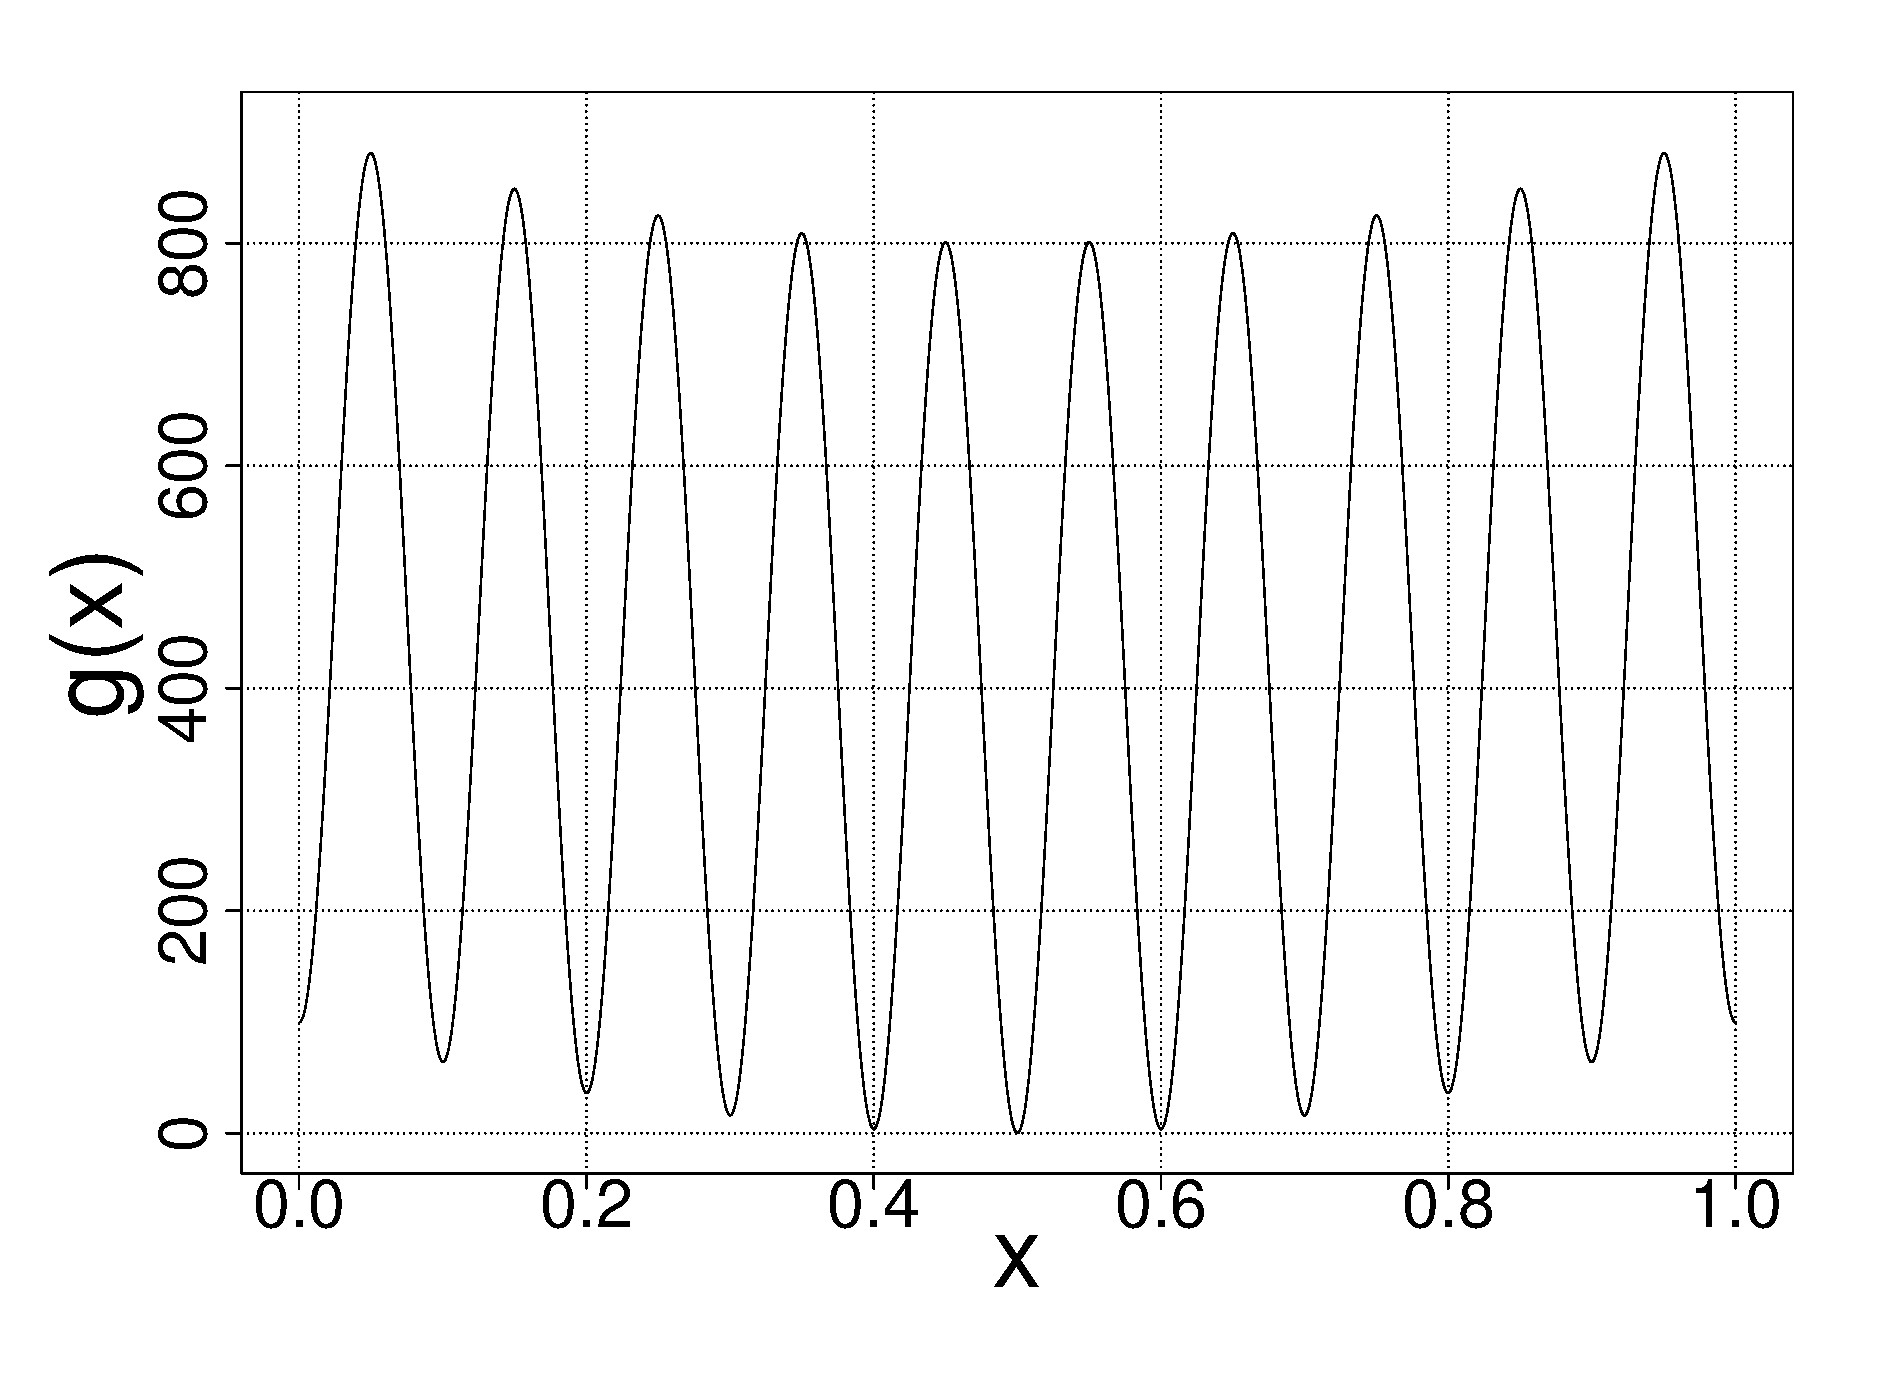
\includegraphics[width=0.65\linewidth]{../figures/DTLZ3_gx.eps}
\end{center}
\setlength{\abovecaptionskip}{-8mm}
\setlength{\belowcaptionskip}{0mm}
\caption{$g(\bm{x}_M)$の推移}
\label{fig:dtlz3_gx}
\end{figure}

\clearpage
\subsubsubsection{DTLZ4}
DTLZ4は  \Eqref{dtlz4}  で表される多目的問題である.
DTLZ2と基本的な構造は同様である.
DTLZ2と大きく違う点は,各目的関数$f_m$内の位置変数$x_1,\cdots,x_{M-1}$が$\alpha$乗となっている点である.
これにより,変数の値の僅かな違いが目的関数の値に大きな影響を与え,解の多様性維持のためには位置変数を高い精度で探索する必要がある.
例として$\alpha=100$の場合の$x^\alpha$と$x$の対応を\Figref{dtlz4_x} に示す.

\Figref{dtlz4_x}より,$x < 0.9$の時,$x^\alpha$はほぼ0となってしまうため,$x > 0.9$を細かく調べる必要がある.
DTLZ4のパレートフロント上の設計変数は,位置変数の$\alpha$乗$x^\alpha _1,\cdots,x^\alpha _{M-1}$が[0,1]に一様に広がっており,$g(\bm{x}_M)$が$0$,すなわちすべての距離変数$x_M,\cdots,x_n$が$0.5$となる.

\begin{eqnarray} 
\left.
\begin{array}{ll}
Min. \quad f_{1}  (\bm{x}) = (1+g(\bm{x}_{M}))\cos({x_{1}}^\alpha\pi/2)  \cdots  \cos({x_{M-2}}^\alpha\pi/2)\cos({x_{M-1}}^\alpha\pi/2),\\
Min. \quad f_{2} (\bm{x}) = (1+g(\bm{x}_{M}))\cos({x_{1}}^\alpha\pi/2)  \cdots  \cos({x_{M-2}}^\alpha\pi/2)\sin({x_{M-1}}^\alpha\pi/2), \\
Min. \quad f_{3} (\bm{x}) = (1+g(\bm{x}_{M}))\cos({x_{1}}^\alpha\pi/2)  \cdots  \sin({x_{M-2}}^\alpha\pi/2), \\
     \  \  \ $\vdots$    \qquad     \qquad      \qquad     \qquad \vdots \\
Min. \quad f_{M}(\bm{x}) = (1+g(\bm{x}_{M}))\sin({x_{1}}^\alpha\pi/2)\\
with \quad g(\bm{x}_{M}) = \sum_{x_i \in \bm{x}_M} (x_i - 0.5)^2  \\
  \qquad    \qquad    \qquad  \quad      0 \le x_{i} \le 1,  for \ i = 1, 2, \ldots, n. \\
        \qquad    \qquad    \qquad  \quad        \bm x = (x_1,x_2, \ldots, x_n)\\
   \qquad    \qquad    \qquad  \quad        \bm{x}_M = (x_M,x_{M+1}, \ldots, x_n)
   \label{dtlz4} 
\end{array}
\right\}
\end{eqnarray}


\begin{figure}[htbp]
\begin{center}
\centering
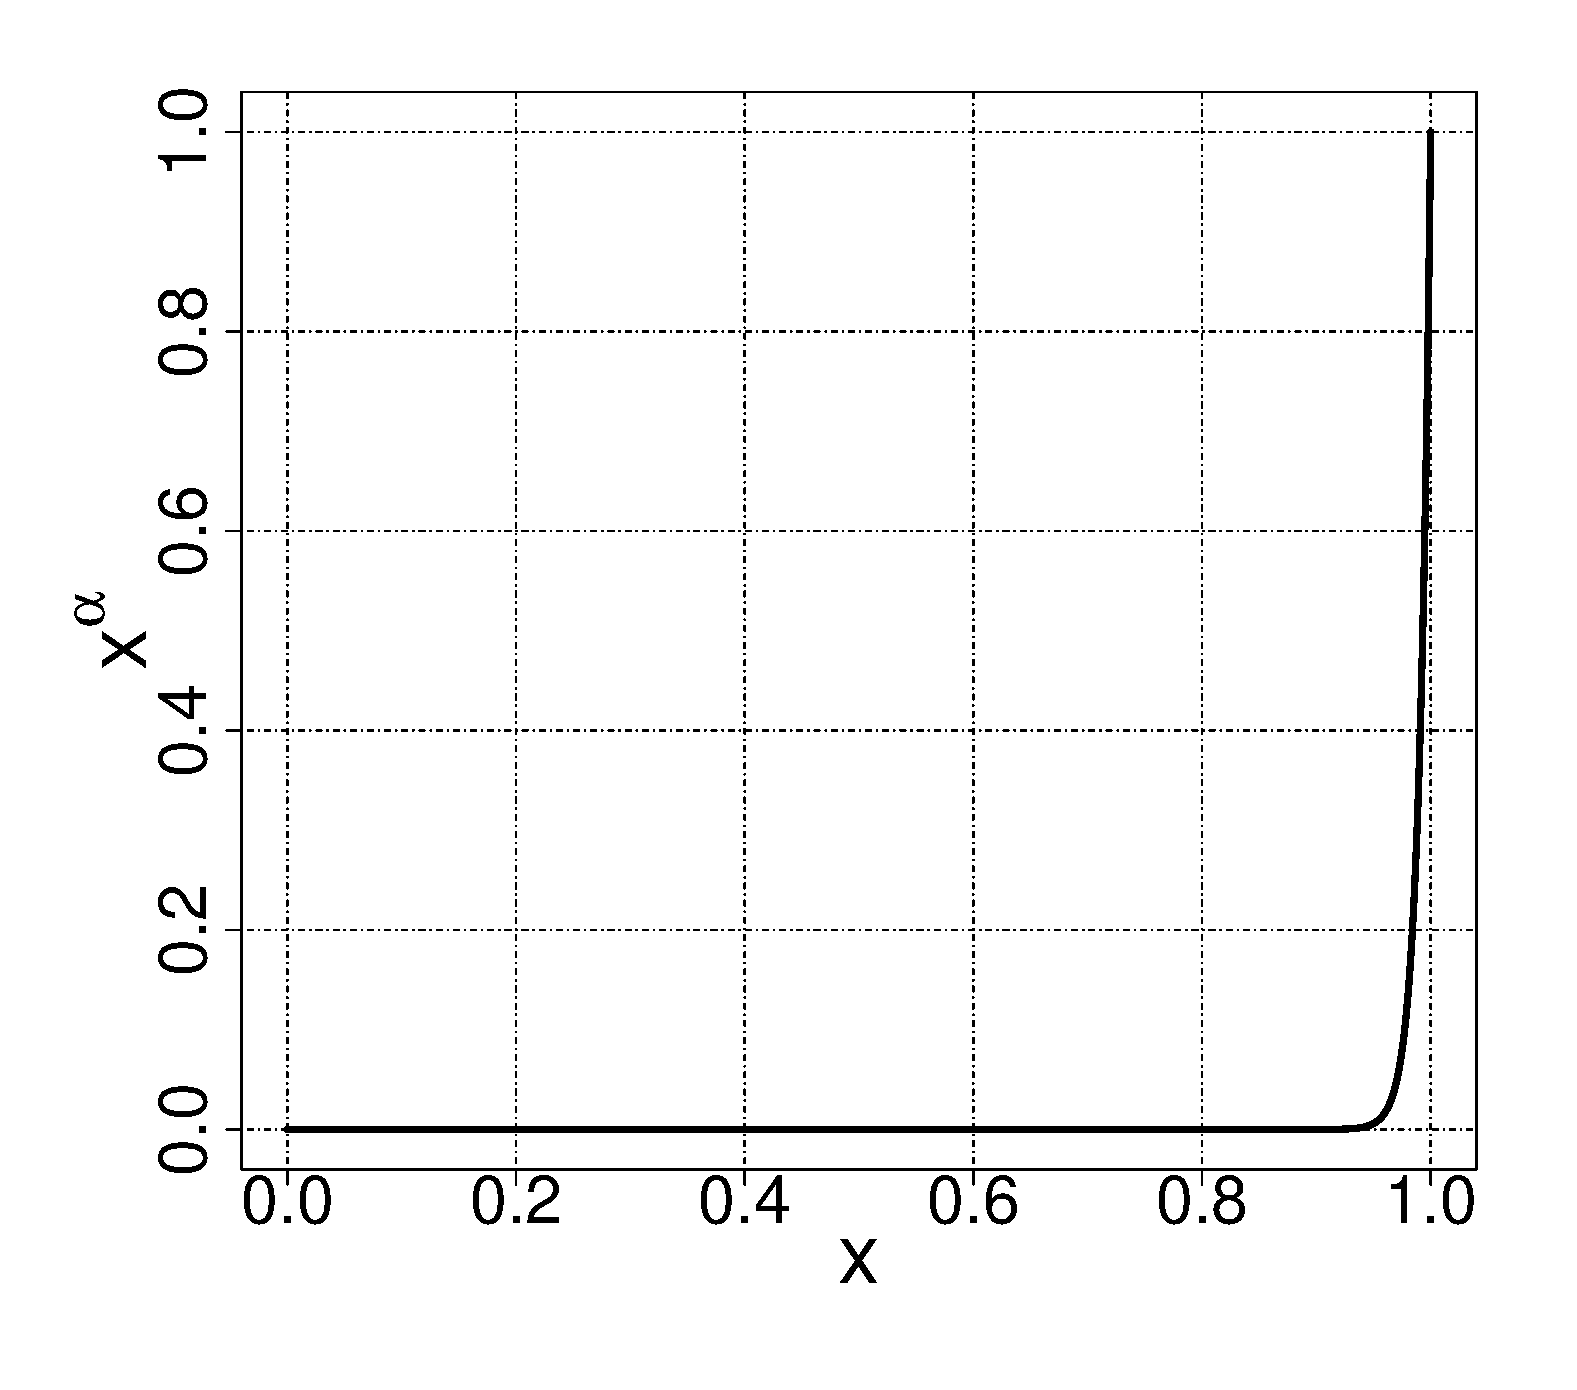
\includegraphics[width=0.4\linewidth]{../figures/dtlz4_position_sensitive.eps}
\end{center}
\setlength{\abovecaptionskip}{-8mm}
\setlength{\belowcaptionskip}{0mm}
\caption{$x$ と$x^ \alpha$の対応}
\label{dtlz4_x}
\end{figure}

%\subsubsection{DTLZ7}
%DTLZ7は  \Eqref{dtlz7}  で表される多目的問題である.
%DTLZ7は,局所解を持たない単峰性の最適化問題であり,$M$目的の最適化問題として定式化した場合,$2^{M-1}$個の非連続な最適解部分を持つ問題である.
%DTLZ2-4と同様に,設計変数$x_1,\cdots,x_{M-1}$は位置変数,設計変数$x_M,\cdots,x_n$は距離変数となるが,DTLZ2-4と異なり,距離変数$x_M$の最適値は$0$である.
%したがって,DTLZ7の真のパレート最適解を得るためには,位置変数$x_1,\cdots,x_{M-1}$が一様に広がっており,すべての距離変数$x_M,\cdots,x_n$が$0$となる必要がある.
%
%\begin{eqnarray} 
%\left.
%\begin{array}{ll}
%Min. \quad f_{1}  (x_1) = x_1,\\
%Min. \quad f_{2} (x_2) = x_2, \\
%Min. \quad f_{3} (x_3) = x_3, \\
%     \  \  \ $\vdots$    \qquad       \qquad \vdots \\
%Min. \quad f_{M_1}(x_{M-1}) = x_{M-1},\\
%Min. \quad f_{M} (\bm x) = (1 + g(\bm{x_M}))h(f_1,f_2,\cdots,f_{M-1},g),\\
%with\ g(\bm{x}_{M}) = 1 + \cfrac{9}{|\bm{x_M}|} \sum_{x_i \in \bm{x_M}} x_i,  \\
%\quad \quad \ h(f_1,f_2,\cdots,f_{M-1},g) = M - \sum^{M-1}_{i = 1}\left[ \cfrac{f_i}{1+g} (1 + sin(3\pi f_i))\right],\\
%   \qquad    \  0 \le x_{i} \le 1,  for\ i = 1, 2, \ldots, n, \\
%      \qquad    \        \bm x = (x_1,x_2, \ldots, x_n),\\
%   \qquad    \        \bm{x}_M = (x_M,x_{M+1}, \ldots, x_n).
%   \label{dtlz7} 
%\end{array}
%\right\}
%\end{eqnarray}
%
\newpage

\subsubsection{WFG問題}
WFG問題\cite{Huband2006AReview}は2006年にHubandらが提案した多目的ベンチマーク問題である.
大きな特徴として,1)設計変数が何度もスケーリングされる,2)設計変数間で相関関係を持つ問題がある,3)真のパレートフロントの形状が複雑であるといった点があげられる.

上述の1点目の性質より,非常に非線形性の強い問題であり,また2点目の性質より設計変数間で相関関係を持つ場合があるため,DTLZ問題と比較し,非常に複雑な構造となっている.

基本的な式の構造は\Eqref{wfg_standard}で表される.

\begin{eqnarray} 
\left.
\begin{array}{rccl}
Min. & f_{m = 1:M}  (\bm{x}) &=& x_M + S_m h_m (x_1, \cdots, x_{M-1})\\
where & \bm{x} &=& \{x_1, \cdots, x_M\} \\
&&=& \{ max(t^p_M,A_1)(t^p_1 - 0.5) + 0.5, \cdots, \\
& & & \ \ max(t^p_M,A_{M-1})(t^p_{M-1} - 0.5)+0.5, t^p_M\} \\
& \bm{t^p} &=& \{t^p_1, \cdots, t^p_M \} \longleftarrow [ \ \bm{t^{p-1}} \longleftarrow [ \ \cdots \longleftarrow [ \ \bm{t^1} \longleftarrow [ \ \bm{z_{[0,1]}}\\
&  \bm{z_{[0,1]}} &=& \{ z_{1,[0,1]}, \cdots, z_{n,[0,1]} \} = \{ z_1 / z_{1,max}, \cdots, z_n / z_{n,max} \}
   \label{wfg_standard} 
\end{array}
\right\}
\end{eqnarray}

\Eqref{wfg_standard}において,$M$は目的関数の数を示している.
$\bm{x}$は目的関数値を定める値で$M$個からなり,$x_1, \cdots, x_{M-1}$が目的関数空間における解の位置を決定する値,$x_M$が目的関数空間における解の原点からの距離を決定する値となる.
$\bm{z}$は,設計変数値を表し,設計変数の数$n$は位置パラメータ$k$と距離パラメータ$l$を足した数となる.
$A_{1:M-1}$は0または1の定数であり問題によって決定される.
$h_{1:M}$はパレートフロントの形状を決定する関数(形状関数),$S_{1:M}$はスケーリングを行う定数である.
$t^{1:p}$は,射影変換された変数を示し,$\longleftarrow$は後述するスケーリング関数を用いて変数を射影することを意味する.

このように,WFG問題では,設計変数$\bm{z}$を何度もスケーリング(射影)し,$t^p$に変換したのち,目的関数値を定める$\bm{x}$を算出し,パレートフロントの形状を決定する関数$h_{1:M}$に与えることで,目的関数値が算出される.

本研究で用いるWFG2,4,6,7で使用される形状関数$h_{1:M}$とスケーリング関数をそれぞれ\Tabref{wfg_shape},\Tabref{wfg_trans}にそれぞれまとめる.

また,WFG2,4,6,7で使用する形状関数$h_{1:M}$とスケーリング関数の組み合わせを\Tabref{wfg_comb}に示す.



\begin{table}[htbp]
\fontsize{9.5pt}{9.5pt} \selectfont
%\tabcolsep = 1pt
\centering
\caption{影響評価で用いるWFG問題で使用される形状関数}
\vspace{0.1cm}
\label{wfg_shape}
\begin{tabular}{|c|}
\hline 
$\bf{Convex}$\\
\hline
$convex_1(x_1, \cdots, x_{M-1}) = \prod^{M-1}_{i=1} (1 - cos(x_i \pi / 2 )) $\\
$convex_{m=2:M-1}(x_1, \cdots, x_{M-1}) =\left( \prod^{M-m}_{i=1} (1 - cos(x_i \pi / 2 )) \right) ( 1 - sin(x_{M-m-1} \pi / 2 ) )$\\
$convex_M(x_1, \cdots, x_{M-1}) = 1 - sin( x_1 \pi / 2 )$\\
%When $h_{m = 1:M} = convex_m$, the Pareto optimal front is purely convex.\\
\hline
\hline
$\bf{Concave}$\\
\hline
$concave_1(x_1, \cdots, x_{M-1}) = \prod^{M-1}_{i=1} (1 - cos(x_i \pi / 2 )) $\\
$concave_{m=2:M-1}(x_1, \cdots, x_{M-1}) =\left( \prod^{M-m}_{i=1} (1 - cos(x_i \pi / 2 )) \right) ( 1 - sin(x_{M-m-1} \pi / 2 ) )$\\
$concave_M(x_1, \cdots, x_{M-1}) = 1 - sin( x_1 \pi / 2 )$\\
%When $h_{m = 1:M} = concave_m$, the Pareto optimal front is purely concave, and a region of the hyper-sphere\\
%of radius one centered at the origin, where $\Sigma^M_{m=1} h^2_m = 1$.\\
\hline
\hline
${\bf Disconnected} (\alpha, \beta > 0, A \in \{1, 2, \cdots \}) $\\
\hline
$disc_M (x_1, \cdots, x_{M-1}) = 1 - (x_1)^\alpha cos^2 (A(x_1)^\beta \pi)$\\
\hline
\end{tabular}
\end{table}


\begin{table}[htbp]
\fontsize{9.5pt}{9.5pt} \selectfont
%\tabcolsep = 1pt
\centering
\caption{影響評価で用いるWFG問題で使用されるスケーリング関数}
\vspace{0.1cm}
\label{wfg_trans}
\begin{tabular}{|c|}
\hline 
${\bf Bias : Parameter Dependent} (A \in (0,1), 0 < B < C)$\\
\hline
$b\_param(y, \bm{y}\prime, A, B, C) = y^{B+(C-B) v ( u (\bm{y} \prime ))}$\\
$v ( u (\bm{y} \prime )) = A - (1 - 2 u (\bm{y} \prime )) \left| \lfloor 0.5 - u (\bm{y} \prime ) \rfloor + A \right|$\\
\hline
\hline
${\bf Shift : Linear} (A \in (0,1))$\\
\hline
$s\_linear(y, A) = \cfrac{|y - A|}{|\lfloor A - y \rfloor + A|}$\\
\hline
\hline
{\bf Shift : Multi-modal} $(A \in \{1, 2, \cdots\}, B \geq 0, (4A + 2)\pi \geq 4B, C \in (0,1)) $\\
\hline
$s\_multi(y, A, B, C) = \cfrac{1 + cos \left[ (4A+2) \pi \left( 0.5 - \cfrac{|y - C|}{2(\lfloor C - y \rfloor + C)} \right) \right] + 4B \left( \cfrac{|y - C|}{2(\lfloor C - y \rfloor + C) }  \right) ^ 2}{B+2}$\\
\hline
\hline
{ \bf Reduction : Weighted Sum} $(|\bm{w}| = |\bm{y}|, w_1, \cdots, w_{|\bm{y}|}) $\\
\hline
$r\_sum (\bm{y}, \bm{w}) =  \left( \Sigma^{|\bm{y}|}_{i=1} w_i y_i \right) / \Sigma^{|\bm{y}|}_{i=1} w_i$\\
\hline
\hline
{\bf Reduction : Non-separable} $(A \in \{1,  \cdots, |\bm{y}| \}, |\bm{y}| \ mod \ A = 0) $\\
\hline
$r\_nonsep (\bm{y}, A) = \cfrac{\Sigma^{|\bm{y}|}_{j=1}\left(  y_j + \Sigma^{A-2}_{k=0} \left| y_j - y_{1 + (j + k) \ mod \  | \bm{y} | } \right| \right)}{\cfrac{|\bm{y}|}{A} \lceil A / 2 \rceil (1 + 2A - 2 \lceil A / 2 \rceil)}$\\
\hline
\end{tabular}
\end{table}

\begin{table}[htbp]
\fontsize{10pt}{10pt} \selectfont
%\tabcolsep = 1pt
\centering
\caption{影響評価で用いるWFG問題の形状関数とスケーリング関数の組み合わせ}
\label{wfg_comb}
\begin{tabular}{|c||c|l|}
\hline
Problem & Type & \multicolumn{1}{c|}{Setting}\\
\hline
All & Constants & $S_{m=1:M} = 2m$\\
&                       & $A_{1:M-1} = 1$ ( for WFG 2, 4, 6 and 7)\\
\hline
All & Domains & $z_{i = 1:n,max} = 2i$\\
\hline
WFG2 & Shape & $h_{m = 1:M-1} = convex_m$\\
           &             & $h_M = disc_M ( with \alpha = \beta = 1 \ and \ A = 5)$\\
           &     $t^1$   & $t^1_{i=1:k} = y_i$\\
           &             &$ t^1_{i = k+1:n} = s\_linear(y_i, 0.35)$\\
           &     $t^2$    & $t^2_{i = 1:k} = y_i$\\
           &             & $t^2_{i = k+1:k+l/2} = r\_nonsep(\{ y_{k+2(i - k) - 1}, y_{k+2(i - k)} \},2)$\\
           &     $t^3$    & $t^3_{i = 1:M-1} = r\_sum(\{ y_{(i-1)k / (M - 1) + 1}, \cdots, y_{ik / (M-1)} \}, \{1, \cdots, 1 \} )$\\
           &              & $t^3_M = r\_sum(\{ y_{k+1}, \cdots, y_{k+l/2} \} , \{ 1, \cdots, 1\} )$\\
\hline
WFG4 & Shape &$ h_{m = 1:M} = concave_m$\\
           &     $ t^1$  & $t^1_{i = 1:n} = s\_multi(y_i , 30, 10, 0.35)$\\
           &  $t^2$      & $t^2_{i = 1:M-1} = r\_sum(\{ y_{(i-1)k / (M - 1) + 1}, \cdots, y_{ik / (M-1)} \}, \{1, \cdots, 1 \} )$\\
           &                 & $t^2_M = r\_sum(\{ y_{k+1}, \cdots, y_n  \}, {1, \cdots, 1})$\\
\hline
WFG6 & Shape & $h_{m = 1:M} = concave_m$\\
           &     $t^1$   & As $t^1$ from WFG2. (Linear shift.)\\
           &     $t^2$    & $t^2_{i = 1:M-1} = r\_nonsep(\{ y_{(i - 1)k/(M-1)+1},\cdots, y_{ik/(M-1)} \}, k/(M-1))$\\
           &             & $t^2_M = r\_nonsep(\{ y_{k+1},\cdots, y_{n} \},l)$\\
\hline
WFG7 & Shape & $h_{m = 1:M} = concave_m$\\
           &     $ t^1$  & $t^1_{i = 1:k} = b\_param(y_i , r\_sum(\{ y_{i+1}, \cdots, y_n \}, \{1, \cdots, 1\}), \cfrac{0.98}{49.98},0.02,50)$\\
           &                 & $ t^1_{i = k+1:n} = y_i$\\
           &     $t^2$   & As $t^1$ from WFG2. (Linear shift.)\\
           &     $t^3$   & As $t^2$ from WFG4. (Weighted sum reduction.)\\
\hline  
%WFG8 & Shape & $h_{m = 1:M} = concave_m$\\
%           &     $ t^1$  & $t^1_{i = 1:k} = y_i$\\
%           &                 & $t^1_{i = k+1:n} = b\_param(y_i , r\_sum(\{ y_{i+1}, \cdots, y_n \}, \{1, \cdots, 1\}), \cfrac{0.98}{49.98},0.02,50)$\\
%           &     $t^2$   & As $t^1$ from WFG2. (Linear shift.)\\
%           &     $t^3$   & As $t^2$ from WFG4. (Weighted sum reduction.)\\
%\hline  
\end{tabular}
\end{table}

\clearpage

\subsubsection{CEC2009問題}
CEC2009問題\cite{Zhang2008Multiobjective}は2009年にZhangらが提案した多目的ベンチマーク問題である.
CEC2009問題は現実の設計問題に近い問題を作成するという意図で提案された.
現実の設計問題に近い構成にするため,設計変数同士に相関を持つことや,制約条件が存在する,真のパレートフロントが不連続な形状をしている等複雑な構成となっていることが特徴である.
CEC2009問題は20種類のベンチマーク問題があり,その内10種類は制約条件付き問題である.
本研究では,制約なしのベンチマーク問題であるUF2,UF9と制約条件付きベンチマーク問題であるCF2,CF7の4つのベンチマーク問題で数値実験を行う.
次節以降でこれら4つのベンチマーク問題について述べる.

\subsubsubsection{UF2}
UF2は制約なしの2目的のベンチマーク問題である.
\Eqref{uf2_eq}にUF2の構成を示す.
設計変数の数$n$は任意に決定することができ,設計変数の探索領域は$[0,1] \times [-1,1]^{n-1}$となる.
%また,真のパレートフロントの形状を\Figref{}に示す.

\begin{eqnarray} 
\left.
\begin{array}{rccl}
Min. &f_1 &=& x_1 + \cfrac{2}{|\bm{J_1}|} \sum_{j \in \bm{J_1}} y^2_j\\
Min. & f_2 &=& 1 - \sqrt{x_1} + \cfrac{2}{|\bm{J_2}|} \sum_{j \in \bm{J_2}} y^2_j\\

where &  \bm{J_1} &=& \{j|j {\rm \ is \ odd \ and \ } 2 \leq j \leq n\}\\
& \bm{J_2} &=& \{j|j {\rm \ is \ even \ and \ } 2 \leq j \leq n\}\\
& y_j &=& \left\{ 
\begin{array}{l}
x_j - [0.3 x^2_1 cos (24 \pi x_1 + \frac{4j\pi}{n}) + 0.6x_1] \\
\qquad \qquad \qquad \qquad \times cos(6 \pi x_1 + \frac{j \pi}{n}) \ \ j \in \bm{J_1}\\
x_j - [0.3 x^2_1 cos (24 \pi x_1 + \frac{4j\pi}{n}) + 0.6x_1]\\
\qquad \qquad \qquad \qquad \times sin(6 \pi x_1 + \frac{j \pi}{n}) \ \ j \in \bm{J_2}\\
\end{array}
\right.
   \label{uf2_eq} 
\end{array}
\right\}
\end{eqnarray}


\subsubsubsection{UF9}
UF9は制約なしの3目的のベンチマーク問題である.
\Eqref{uf9_eq}にUF9の構成を示す.
設計変数の数$n$は任意に決定することができ,設計変数の探索領域は$[0,1]^2 \times [-2,2]^{n-2}$となる.

\begin{eqnarray} 
\left.
\begin{array}{rccl}
Min. & f_1 &=& 0.5[max\{0, (1 + \epsilon)(1 - 4(2x_1 - 1)^2)\} + 2x_1]x_2 \\
                     &&&                             + \cfrac{2}{|\bm{J_1}|} \sum_{j \in \bm{J_1}}(x_j - 2x_2 sin(2 \pi x_1 + \cfrac{j \pi}{n} ))^2\\
Min. & f_2 &=& 0.5[max\{0, (1 + \epsilon)(1 - 4(2x_1 - 1)^2)\} - 2x_1 + 2]x_2 \\
                      &&&                             + \cfrac{2}{|\bm{J_2}|} \sum_{j \in \bm{J_2}}(x_j - 2x_2 sin(2 \pi x_1 + \cfrac{j \pi}{n} ))^2\\
Min. & f_3 &=& 1-x_2 \\
                                            &&&+ \cfrac{2}{|\bm{J_3}|} \sum_{j \in \bm{J_3}}(x_j - 2x_2 sin(2 \pi x_1 + \cfrac{j \pi}{n} ))^2\\

where &  \bm{J_1} &=& \{j|3 \leq j \leq n, {\rm \ and \ } j - 1 {\rm \ is \ a \ multiplication \ of \ \ } 3\}\\
& \bm{J_2} &=& \{j|3 \leq j \leq n, {\rm \ and \ } j - 2 {\rm \ is \ a \ multiplication \ of \ \ } 3\}\\
& \bm{J_3} &=& \{j|3 \leq j \leq n, {\rm \ and \ } j {\rm \ is \ a \ multiplication \ of \ \ } 3\}\\
&  \epsilon &=& 0.1

   \label{uf9_eq} 
\end{array}
\right\}
\end{eqnarray}

\subsubsubsection{CF2}
CF2は1制約2目的のベンチマーク問題である.
\Eqref{cf2_eq}にCF2の構成を示す.
設計変数の数$n$は任意に決定することができ,設計変数の探索領域は$[0,1] \times [-1,1]^{n-1}$となる.

\begin{eqnarray} 
\left.
\begin{array}{rccl}
Min. & f_1 &=& x_1 + \cfrac{2}{|\bm{J_1}|} \sum_{j \in \bm{J_1}}(x_j - sin(6\pi x_1 + \cfrac{j\pi}{n}))^2\\
Min. &f_2 &=& 1 - \sqrt{x_1} + \cfrac{2}{|\bm{J_2}|} \sum_{j \in \bm{J_2}} (x_j - cos(6\pi x_1 + \cfrac{j\pi}{n}))^2\\

where &  \bm{J_1} &=& \{j|j {\rm \ is \ odd \ and \ } 2 \leq j \leq n\}\\
& \bm{J_2} &=& \{j|j {\rm \ is \ even \ and \ } 2 \leq j \leq n\}\\
const. & c_1(\bm x) & = &\cfrac{t}{1 + e^{4|t|}} \geq 0\\
where & t &=& f_2 + \sqrt{f_1} - a sin[N\pi (\sqrt{f_1} - f_2 + 1)] - 1\\
   \label{cf2_eq} 
\end{array}
\right\}
\end{eqnarray}


\subsubsubsection{CF7}
CF7は2制約2目的のベンチマーク問題である.
\Eqref{cf7_eq}にCF7の構成を示す.
設計変数の数$n$は任意に決定することができ,設計変数の探索領域は$[0,1] \times [-2,2]^{n-1}$となる.

\begin{eqnarray} 
\left.
\begin{array}{rccl}
Min. & f_1 &=& x_1 + \sum_{j \in \bm{J_1}} h_j(y_j)\\
Min. & f_2 &=& (1 - x_1)^2 + \sum_{j \in \bm{J_2}} h_j(y_j)\\
where &  \bm{J_1} &=& \{j|j {\rm \ is \ odd \ and \ } 2 \leq j \leq n\}\\
           & \bm{J_2} &=& \{j|j {\rm \ is \ even \ and \ } 2 \leq j \leq n\}\\
           & y_j &=& \left\{ 
\begin{array}{l}
x_j - cos (6 \pi x_1 + \frac{j\pi}{n}) \ \ j \in \bm{J_1}\\
x_j - sin (6 \pi x_1 + \frac{j\pi}{n}) \ \ j \in \bm{J_2}\\
\end{array}
\right. \\
&h_2(t) &=& h_4(t) = t^2\\
&h_j(t) &=& 2t^2 - cos(4\pi t) + 1 \ \ \ {\rm for \ } \ j = 3,5,6, \cdots, n \\
const. & c_1(\bm x) &=& x_2 - sin(6 \pi x_1 + \cfrac{2\pi}{n}) \\
                        &&&      - Sgn(0.5(1-x_1) - (1-x_1)^2)\\
                        &&& \times \sqrt{|0.5(1-x_1) - (1-x_1)^2|} \geq 0\\
&    c_2(\bm x) & = &x_4 - sin(6\pi x_1 + \cfrac{4\pi}{n}) \\
                    &&& - Sgn(0.25\sqrt{1-x_1} - 0.5(1-x_1))\\
                    &&& \times \sqrt{|0.25 \sqrt{1-x_1} - 0.5(1-x_1)|} \geq 0\\
   \label{cf7_eq} 
\end{array}
\right\}
\end{eqnarray}

\newpage

\subsubsection{CDTLZ問題}
CDTLZ問題\cite{Jain2014Evolutionary2}は2014年にJainらによって提案された制約条件付きのベンチマーク問題である.
CDTLZ問題はDebらが考案したDTLZ問題に制約条件を追加した問題であり,6つの問題が提案されている.
CDTLZ問題では,3種類の制約条件の問題が用意されている.

C1シリーズの問題は,オリジナルのDTLZ問題の真のパレートフロントを覆うように実行不可能領域が存在する問題であり,実行不可能領域を越えなければ真のパレートフロントに到達できないため,実行不可能領域と実行可能領域の境界付近に局所最適解が生成されやすい.
C2シリーズの問題は,オリジナルのDTLZ問題の真のパレートフロント上に部分的に実行不可能領域が存在する問題であり,真のパレートフロントの形状が不連続となる.
C3シリーズの問題は,オリジナルのDTLZ問題の真のパレートフロントが実行不可能領域に存在する問題であり,実行可能領域と実行不可能領域の境界線が真のパレートフロントとなる.

本研究では,C1DTLZ3,C2DTLZ2 convex,C3DTLZ1の3つの問題を数値実験に使用した.
次節以降でこれらの問題について説明する.

\subsubsubsection{C1DTLZ3}
C1DTLZ3はDTLZ3に1つ制約条件を追加したベンチマーク問題である.
真のパレートフロントを覆うように実行不可能領域が存在し,実行可能領域と実行不可能領域の境界付近に局所最適解が生成されやすい問題となっている.
C1DTLZ3で追加された制約条件を\Eqref{c1dtlz3_const}に示す.
本実験では$r$を$9$とした.

\begin{equation}
\centering
c(\bm{x}) = \left( \sum^M_{i=1} f_i (\bm{x})^2 - 16 \right) \left( \sum^M_{i=1} f_i(x)^2 - r^2 \right) \geq 0
\label{c1dtlz3_const}
\end{equation}


\subsubsubsection{C2DTLZ2 convex}
C2DTLZ2 convexはDTLZ2のパレートフロントの形状を凹型から凸型に変更し,1つ制約条件をを追加したベンチマーク問題である.
真のパレートフロント上に部分的に実行不可能領域が存在し,実行可能な真のパレートフロントの形状は不連続となっている.
C2DTLZ convexで変更された目的関数の射影変換を\Eqref{c2dtlz2_changed}に,追加された制約条件を\Eqref{c2dtlz2_const}に示す.
本実験では$r$を$0.225$とした.

\begin{eqnarray}
\left.
\begin{array}{rcl}
f_i &\longleftarrow& f^4_i \ \ \ \ i = 1, 2, \cdots, M-1\\
f_M &\longleftarrow& f^2_M
\end{array}
\right\}
\label{c2dtlz2_changed}
\end{eqnarray}

\begin{eqnarray}
\left.
\begin{array}{rcl}
c(\bm{x}) &=& \sum^M_{i=1} (f_i(\bm{x}) - \lambda)^2 - r^2 \geq 0\\
where \ \ \lambda &=& \cfrac{1}{M} \sum^M_{i=1} f_i(\bm{x})\\
\end{array}
\right\}
\label{c2dtlz2_const}
\end{eqnarray}

\subsubsubsection{C3DTLZ1}
C3DTLZ1はDTLZ1に目的関数の数$M$だけ制約条件を追加したベンチマーク問題である.
DTLZ1の真のパレートフロントが実行不可能領域にあり,実行可能領域と実行不可能領域の境界線がパレート最適解となる問題である.
C3DTLZ1で追加された制約条件を\Eqref{c3dtlz1_const}に示す.

\begin{equation}
c_j(\bm{x}) = \sum^M_{i = 1, i \neq j} f_j(\bm{x}) + \cfrac{f_i(\bm x)}{0.5} - 1 \geq 0 \ \ \ \ \ \forall j = 1, 2, \cdots, M
\label{c3dtlz1_const}
\end{equation}

\newpage

\subsubsection{Engineering問題}
本実験では現実の設計問題に則したEngineering問題としてCar Side Impact問題\cite{Jain2014Evolutionary2}とWelded Beam Design問題\cite{Deb2006Reference}を用いて数値実験を行った.
次節以降でこれらの問題について述べる.

\subsubsubsection{Car Side Impact}
Car Side Impact問題は,3目的の最小化最適化問題である.
各目的関数にはトレードオフの関係があり,10個の制約条件と7つの設計変数を持つ問題である.
Car Side Impact問題は\Eqref{car_eq}で表される.

\subsubsubsection{Welded Beam Design}
Welded Beam Design問題は,2目的の最小化最適化問題である.
各目的関数にはトレードオフの関係があり,4個の制約条件と4つの設計変数を持つ問題である.
Welded Beam Design問題は\Eqref{wbd_eq}で表される.

\begin{eqnarray}
\left.
\begin{array}{rccl}
Min. & f_1(\bm x) &=& 1.98 + 4.9 x_1 + 6.67x_2 + 6.98x_3 + 4.01x_4 + 1.78x_5 \\ 
        &                   &  & + 0.00001x_6 + 2.73x_7\\
Min. & f_2(\bm x) &=& F\\
Min. & f_3(\bm x) &=& 0.5(V_{MBP} + V_{FD})\\
const. &c_1(\bm x) &=& 1.16 - 0.3717x_2x_4 - 0.0092928x_3 \leq 1\\
          & c_2(\bm x) &=& 0.261 - 0.0159x_1x_2 - 0.006486x_1 - 0.019x_2x_7 \\
          &                    &  &+ 0.0144x_3x_5 + 0.0154464x_6 \leq 0.32\\
          & c_3(\bm x) &=& 0.214 + 0.00817x_5 - 0.045195x_1 - 0.0135168x_1 \\
          &                    &   &+ 0.03099x_2x_6 - 0.018x_2x_7 + 0.007176x_3 + 0.023232x_3 \\
          &                    &   &- 0.00364x_5x_6 - 0.018x_2^2 \leq 0.32\\
          & c_4(\bm x) &=& 0.74 - 0.61x_2 - 0.031296x_3 - 0.031872x_7 \\
          &                    &  &+ 0.227x_2^2 \leq 0.32\\
          & c_5(\bm x) &=& 28.98 + 3.818x_3 - 4.2x_1x_2 + 1.27296x_6 \\
          &                   &   &- 2.68065x_7 \leq 32\\
          & c_6(\bm x) &=& 33.86 + 2.95x_3 - 5.057x_1x_2 - 3.795x_2 \\
          &                   &   &- 3.4431x_7 + 1.45728 \leq32\\
          & c_7(\bm x) &=& 44.36 - 9.9x_2 - 4.4505x_1 \leq 32\\
          & c_8(\bm x) &\equiv & F = 4.72 - 0.5x_4 - 0.19x_2x_3 \leq4\\
          & c_9(\bm x) & \equiv & V_{MBP} = 10.58 - 0.674x_1x_2 - 0.067275x_2 \leq 9.9\\
          & c_{10}(\bm x) & \equiv & V_{FD} = 16.45 - 0.489x_3x_7 - 0.843x_5x_6 \leq 15.7\\
where & & & 0.5 \leq x_1 \leq 1.5, 0.45 \leq x_2 \leq 1.35, 0.5 \leq x_3 \leq 1.5\\
           & & & 0.5 \leq x_1 \leq 1.5, 0.875 \leq x_5 \leq 2.625, 0.4 \leq x_6 \leq 1.2,\\
           & & & 0.4 \leq x_7 \leq 1.2\\
\end{array}
\right\}
\label{car_eq}
\end{eqnarray}

\begin{eqnarray}
\left.
\begin{array}{rccl}
Min. & f_1(\bm x) &=& 1.10471h^2l + 0.04811tb(14.0 + l) \\ 
Min. & f_2(\bm x) &=& \cfrac{2.1952}{t^3b}\\
const. &c_1(\bm x) &\equiv& 13,600 - \tau(\bm x) \geq 0\\
          & c_2(\bm x) &\equiv& 30,000 - \sigma(\bm x) \geq 0 \\
          & c_3(\bm x) &\equiv& b-h \geq 0 \\
          & c_4(\bm x) &\equiv& P_c(\bm x) - 6,000 \geq 0\\

where &\tau(\bm x) & = & \sqrt{(\tau^\prime) + (\tau^{\prime \prime})^2 + (l \tau^\prime \tau^{\prime \prime}) / \sqrt{0.25(l^2 + (h+t)^2)}}\\
           &\tau^\prime & = & \cfrac{6,000}{\sqrt{2}hl}\\
           &\tau^{\prime \prime} &=& \cfrac{6,000(14 + 0.5l)\sqrt{0.25(l^2 + (h+t)^2)}}{2\{0.707hl(l^2/12+0.25(h+t)^2)\}}\\
           &\sigma(\bm x) &=& \cfrac{504,000}{t^2b}\\
           &P_c(\bm x) &=& 64,746.022(1-0.0282346t)tb^3\\
           & \bm x &=& (h, b, l, t)\\
           & & & 0.125 \leq h,b \leq 5.0, 0.1 \leq l,t \leq 10.0\\
\end{array}
\right\}
\label{wbd_eq}
\end{eqnarray}

\newpage

\subsubsection{Modified DTLZ問題}
%Modified DTLZ問題\cite{}は2017年に近藤らによって提案されたベンチマーク問題である.
Modified DTLZ問題はDebらが考案したDTLZ問題を改変したものであり,3つの問題が提案されている.
オリジナルのDTLZ問題では上述の通り距離変数が0.5となった時に真のパレートフロントに到達する.
しかし,これでは設計変数の小数点以下の桁数を小さくするほど,真の最適値に用意に収束してしまうと考えられる.
Modified DTLZ問題では,距離変数の最適値を無理数に変更することで,小数点以下の桁数を粗くしただけでは収束しづらい問題となっている.
次節よりModified DTLZ2-4について述べる.

\subsubsubsection{Modified DTLZ2, 4}
Modified DTLZ2,4は,DTLZ2,4の距離変数の最適値を$0.5$から無理数である$0.1\pi$に変更したものである.
DTLZ2,4では$g(\bm x)$は\Eqref{gx_dtlz2}で定義される.

\begin{equation}
\centering
g(\bm x_M) = \sum_{x_i \in \bm x_M} (x_i - 0.5)^2
\label{gx_dtlz2}
\end{equation}

$M$は目的関数の数を,$\bm x$は設計変数を示している.
$\bm x_M$は,設計変数の中でも距離変数と呼ばれる変数を表し,目的関数空間での真のパレートフロントまでの距離を決定する.
DTLZ2とDTLZ4では,距離変数$\bm x_M$がすべて$0.5$に収束したとき,真のパレートフロントに到達する.
上述の通り,これでは設計変数の小数点以下の桁数を小さくするほど,真の最適値に用意に収束してしまうと考えられる.
そこで,小数点以下の桁数を粗くしただけでは収束しづらいよう$g(\bm x_M)$を\Eqref{gx_mod2}とし,距離変数$\bm x_M$がすべて$0.1\pi$という無理数に収束しなければ,パレートフロントに到達しないように改変されている.

\begin{equation}
\centering
g(\bm x_M) = \sum_{x_i \in \bm x_M} (x_i - 0.1 \pi)^2
\label{gx_mod2}
\end{equation}

\subsubsubsection{Modified DTLZ3}
Modified DTLZ3はDTLZ3の距離変数の最適値を$0.5$から無理数である$0.1 \pi$に変更したものである.
Modified DTLZ2,4と同様に,\Eqref{gx_dtlz3}で定義される$g(\bm x_M)$より,距離変数の最適値が$0.5$となっている.
これを\Eqref{gx_mod3}に改変することで,距離変数の最適値を無理数に変更する.

\begin{equation}
\centering
g(\bm x_M) = 100[|\bm x_M| + \sum_{x_i \in \bm x_M} (x_i - 0.5)^2 - cos(20 \pi (x_i - 0.5 ))]
\label{gx_dtlz3}
\end{equation}

\begin{equation}
\centering
g(\bm x_M) = 100[|\bm x_M| + \sum_{x_i \in \bm x_M} (x_i - 0.1\pi)^2 - cos(20 \pi (x_i - 0.1 \pi ))]
\label{gx_mod3}
\end{equation}

%\newpage


%\subsubsection{Multi DTLZ問題}
%Multi DTLZ問題は近藤らの提案したModified DTLZ問題をさらに改変したものである.
%Modified DTLZ問題は距離変数の最適値が$0.1\pi$の1つだけである.
%現実の設計問題を考えた場合,最適値が2つ以上存在する場合などが考えられるが,このような問題のベンチマーク問題は少ない.
%そこで,Modified DTLZ問題を改変することで,最適値が2つとなる問題を提案する.
%次節から,Multi DTLZ2,3,4について述べる.
%
%\subsubsubsection{Multi DTLZ2,4}
%Multi DTLZ2,4はそれぞれModified DTLZ2,4を改変したものである.
%上述の\Eqref{gx_mod2}より,Modified DTLZ2,4は距離変数の最適値が$0.1\pi$の1点である.
%Multi DTLZ2,4では\Eqref{gx_mod2}を\Eqref{gx_multi2}に改変することで距離変数の最適値が$0.1\pi$と$0.3\pi$の2点となる.
%
%\begin{eqnarray}
%g(\bm x_M) = 
%\left\{
%\begin{array}{rl}
%\sum_{x_i \in \bm x_M} (x_i - 0.1 \pi)^2 & if  \ \ \  0 \leq x_i < 0.5\\
%\sum_{x_i \in \bm x_M} (x_i - 0.3 \pi)^2 & otherwise \\
%\end{array}
%\right.
%\label{gx_multi2}
%\end{eqnarray}
%

%\subsubsection{Multi DTLZ3}
%Multi DTLZ3はModified DTLZ3を改変したものである.
%上述の\Eqref{gx_mod3}より,Modified DTLZ3は距離変数の最適値が$0.1\pi$の1点である.
%Multi DTLZ3では\Eqref{gx_mod3}を\Eqref{gx_multi3}に改変することで距離変数の最適値が$0.1\pi$と$0.3\pi$の2点となる.
%
%\begin{eqnarray}
%g(\bm x_M) = 
%\left\{
%\begin{array}{ll}
%100[|\bm x_M| + \sum_{x_i \in \bm x_M} (x_i - 0.1\pi)^2 &\\
%\qquad \qquad \qquad \qquad - cos(20 \pi (x_i - 0.1 \pi ))] & if  \  0 \leq x_i < 0.5 \\
%100[|\bm x_M| + \sum_{x_i \in \bm x_M} (x_i - 0.3\pi)^2 &\\
%\qquad \qquad \qquad \qquad - cos(20 \pi (x_i - 0.3 \pi ))] & otherwise \\
%\end{array}
%\right.
%\label{gx_multi3}
%\end{eqnarray}


\subsection{計算条件}
本実験では,RCGAにおける設計変数の離散化の影響を明らかにするために,代表的なRCGAであるNSGA-IIとMOEA/Dを用いて評価を行う.
\Tabref{tbl:nsga_condition_yobi},\ref{tbl:moead_condition_yobi}にはそれぞれNSGA-IIとMOEA/Dで使用したパラメータをまとめた.
また,集団サイズや世代数,目的関数の数,設計変数の数等は各ベンチマーク問題ごとに設定した.
詳しくは次節以降で説明する.
本研究では,設計変数の小数点以下の桁数を制御することで設計変数を離散化している.
影響評価に用いる比較対象は小数点以下2,4,6,8,16桁で制御したものとする.
また,NSGA-II,MOEA/Dともに交叉と突然変異の後に離散化制御を行うこととする.


\begin{table}[htbp]
\begin{tabular}{lcr}
\begin{minipage}{0.49\hsize}
\centering
\caption{影響評価で用いるNSGA-IIの共通パラメータ}
\label{tbl:nsga_condition_yobi}
\begin{tabular}{c|c}
\hline 
parameter & value \\
\hline 
Crossover rate & $1.0$\\
Mutation rate & $1/n$\\
$\eta_c$ & $30$ \\
$\eta_m$ & $20$ \\
Trial & $10$\\
\hline
\end{tabular}
\\
{\footnotesize $n$ is the number of variables.}\\
{\footnotesize $\eta_c$ and $\eta_m$ are indices of simulated binary crossover and polynomial mutation respectively.}
\end{minipage}

\begin{minipage}{0.49\hsize}
\centering
\caption{影響評価で用いるMOEA/Dの共通パラメータ}
\label{tbl:moead_condition_yobi}
\begin{tabular}{c|c}
\hline 
parameter & value \\
\hline 
Crossover rate & $1.0$\\
Mutation rate & $1/n$\\
$\eta_c$ & $20$ \\
$\eta_m$ & $20$ \\
Neighborhood size & $20$\\
Decomposition Approach & Tchebycheff\\
Trial & $10$\\
\hline
\end{tabular}
\\
{\footnotesize $n$ is the number of variables.}\\
{\footnotesize $\eta_c$ and $\eta_m$ are indices of simulated binary crossover and polynomial mutation respectively.}
\end{minipage}
\end{tabular}
\end{table}


\section{数値実験の結果と考察}
\subsection{NSGA-IIの結果}
\Tabref{tbl:gd_nsgaii}はNSGA-IIにおいて,各ベンチマーク問題における各制御(小数点以下2,4,6,8,16桁)で得られたGDの平均値の推移を示している.
多目的最適化では,最終世代の結果だけではなく収束速度も重要であるため,GDの平均値は10世代目,最終世代の半分,最終世代での結果を示している.
表中に示す Obj. は目的関数の数,Var. は設計変数の数,Gen は GD の平均値を求めた世代数を示している.
また,各世代において最小値となっている値は太字で示した.

\Tabref{tbl:gd_nsgaii}より,ほとんどの問題において桁数が小さいほど(粗く離散化するほど)最終的なGDは小さい値となっていることが分かる.
GDは値が小さいほど解の収束性が良いことを表す指標であることから,桁数が小さいほど(粗く離散化するほど),多くの問題でも解の収束性が向上する傾向があることが確認された.
DTLZ問題では,早い世代から小さいGD値となっており,粗く離散化することで最終的な収束だけでなく収束速度が向上することが分かった.
WFG2やWFG4は小さい桁数では収束性が向上していないことが分かる.
これらの問題では,設計変数空間が大きいため,小数点以下の桁数を変えることが探索にあまり影響しないことが考えられる.

統計的な有意差があるか確認するため,有意水準5\%でWilcoxon の順位和検定を用いて2桁の結果と16桁の結果の比較を行った.
その結果,DTLZ2-4,UF9,CF2,CF7,C1DTLZ3,C2DTLZ2 convex,C3DTLZ1,Welded Beam Design 問題,Modified DTLZ2-4で統計的な有意差が確認された.
上述のWFG2やWFG4では有意差はなかったことから,粗く離散化することで,細かい粒度を用いた探索と比べ,同等かそれ以上の収束性能が得られることが,様々な特徴を持つベンチマーク問題からも確認された.

\Tabref{tbl:igd_nsgaii}はNSGA-IIにおいて,各ベンチマーク問題における各制御(小数点以下2,4,6,8,16桁)で得られたIGDの平均値の推移を示している.
表の見方は\Tabref{tbl:gd_nsgaii}と同様である.
\Tabref{tbl:igd_nsgaii}より,DTLZ2,DTLZ3,UF,CDTLZでは桁数が小さいほど(粗く離散化するほど)IGDは小さくなっていることが分かる.
IGDは値が小さいほど解の収束性・多様性が良いことを表す指標であることから,桁数が小さいほど(粗く離散化するほど)これらのベンチマーク問題では解の多様性も向上していることが分かる.
しかしながら,DTLZ4やModified DTLZ4では桁数が小さいほど悪い結果となっており,桁数が大きいものの方が良い結果となっている.
これは先行研究でも触れたように,DTLZ4の式の構造上,目的関数の位置を司る変数(位置変数)に高い精度がなければ解が多様に広がらないからである.
したがって,問題によって多様性を維持するためには必要最低限の桁数が存在することが分かった.


\begin{table*}[htbp]
\fontsize{7.5pt}{7.5pt} \selectfont
\tabcolsep = 1.5pt
\centering
\caption{制御桁数の違いによるGDの平均値の推移(NSGA-II)}
\label{tbl:gd_nsgaii}
\begin{tabular}{c|ccccc|c|c|c|c|c}
\hline 
problem & MG & PS & Obj. & Var. & Gen & 2-digit & 4-digit & 6-digit & 8-digit & 16-digit \\ 
\cline{7-11}
&&&&&&GD&GD&GD&GD&GD\\
\hline
\multirow{3}{*}{DTLZ2} &        &  & &     & 10 & \bf{1.647} &   1.756 &  1.766 &  1.759 & 1.759\\
  				   & 100 & 100 & 3 & 38 & 50 &$\bf{1.576 \times 10^{-1}}$ &  $2.247 \times 10^{-1}$ & $2.414 \times 10^{-1}$ & $2.595 \times 10^{-1}$ & $2.565 \times 10^{-1}$\\
				   &        &     &           &   &100 & $\bf{5.525 \times 10^{-2}}$ & $1.576 \times 10^{-1}$ & $9.490 \times 10^{-2}$ & $1.003 \times 10^{-1}$ & $1.011 \times 10^{-1}$\\
\hline
\multirow{3}{*}{DTLZ3} &     &&   &       & 10 & $\bf{2.191 \times 10^{3}}$ & $2.508 \times 10^{3}$ &  $2.518 \times 10^{3}$ & $2.512 \times 10^{3}$ & $2.508 \times 10^{3}$\\
  				   & 200 & 500 & 3 & 38 &100 & $\bf{9.935 \times 10}$ & $2.230 \times 10^{2}$ &  $2.878 \times 10^{2}$ & $3.154 \times 10^{2}$ & $4.039 \times 10^{2}$\\
				   &        &   &&     &200 & \bf{6.521} & $4.580 \times 10$ &  $5.622 \times 10$ & $6.196 \times 10$ & $6.669 \times 10$\\

\hline
\multirow{3}{*}{DTLZ4} &        &     &&  & 10 & $\bf{8.213 \times 10^{-1}}$ & 1.286 & 1.216 & 1.223 & 1.223\\
  				   & 100 & 300 & 3&38& 50 & $\bf{1.910 \times 10^{-2}}$ & $5.531 \times 10^{-2}$ & $6.576 \times 10^{-2}$ & $6.889 \times 10^{-2}$ & $7.147 \times 10^{-2}$\\
				   &        &     &&   &100 & $\bf{1.101 \times 10^{-2}}$ & $1.819 \times 10^{-2}$ & $2.320 \times 10^{-2}$ & $2.363 \times 10^{-2}$ & $2.522 \times 10^{-2}$\\
\hline
\multirow{3}{*}{UF2} &        &    &&   & 10 &$\bf{2.978 \times 10^{-1}}$ & $3.106 \times 10^{-1}$ & $3.149 \times 10^{-1}$ & $3.001 \times 10^{-1}$ & $3.001 \times 10^{-1}$\\
  				   & 200 & 200 & 2 & 20 & 100 &$2.639 \times 10^{-2}$ & $\bf{2.312 \times 10^{-2}}$ & $2.362 \times 10^{-2}$ & $2.451 \times 10^{-2}$ & $2.640 \times 10^{-2}$\\
				   &        &      &&  &200 & $1.573 \times 10^{-2}$ & $\bf{1.349 \times 10^{-2}}$ & $1.573 \times 10^{-2}$ & $1.532 \times 10^{-2}$ & $1.701 \times 10^{-2}$\\

\hline
\multirow{3}{*}{UF9} &        &      && & 10& 3.063 & 3.048 & 2.695 & \bf{2.684} & \bf{2.684}\\
  				   & 300 & 200 & 3 &20 &150 & $6.940 \times 10^{-1}$ & $\bf{5.745 \times 10^{-1}}$ & $6.584 \times 10^{-1}$ & $6.003 \times 10^{-1}$ & $6.425 \times 10^{-1}$\\
				   &        &      &&  &300   &$\bf{4.206 \times 10^{-1}}$ &  $4.518 \times 10^{-1}$ & $4.892 \times 10^{-1}$ & $4.470 \times 10^{-1}$ & $4.389 \times 10^{-1}$\\
\hline
\multirow{3}{*}{WFG2} &        &   &&  10  & 10 & $2.350 \times 10^{-1}$ & $\bf{2.218 \times 10^{-1}}$ & $2.428 \times 10^{-1}$ & $2.428 \times 10^{-1}$ & $2.428 \times 10^{-1}$\\
  				   & 100 & 100 & 3 & ($k=6$) &50 & $\bf{6.324 \times 10^{-2}}$ & $7.273 \times 10^{-2}$ & $6.490 \times 10^{-2}$ & $7.088 \times 10^{-2}$ & $7.141 \times 10^{-2}$\\
				   &        &      && ($l=4$) &100 & $4.277 \times 10^{-2}$ & $4.745 \times 10^{-2}$ & $4.516 \times 10^{-2}$ & $4.530 \times 10^{-2}$ & $\bf{4.220 \times 10 ^{-2}}$\\
\hline
\multirow{3}{*}{WFG4} &        &   &&  10  & 10 & $2.249 \times 10^{-1}$ & $2.178 \times 10^{-1}$ & $2.143 \times 10^{-1}$ & $\bf{2.134 \times 10^{-1}}$ & $\bf{2.134 \times 10 ^{-1}}$\\
  				   & 100 & 100 & 3 & ($k=6$) & 50 & $9.867 \times 10^{-2}$ & $9.530 \times 10^{-2}$ & $9.935 \times 10^{-2}$ & $9.563 \times 10^{-2}$ & $\bf{9.510 \times 10 ^{-2}}$\\
				   &        &     && ($l=4$)  &100 & $6.772 \times 10^{-2}$ & $6.628 \times 10^{-2}$ & $6.678 \times 10^{-2}$ & $\bf{6.619 \times 10^{-2}}$ & $6.654 \times 10 ^{-2}$\\
\hline
\multirow{3}{*}{WFG6} &        &  &&  10   & 10 & $3.896 \times 10^{-1}$ & $3.611 \times 10^{-1}$ & $3.592 \times 10^{-1}$ & $\bf{3.560 \times 10^{-1}}$ & $\bf{3.560 \times 10 ^{-1}}$\\
  				   & 100 & 100 & 3 & ($k=6$) & 50  & $1.545 \times 10^{-1}$ & $\bf{1.432 \times 10^{-1}}$ & $1.590 \times 10^{-1}$ & $1.653 \times 10^{-1}$ & $1.653 \times 10^{-1}$\\
				   &        &      && ($l=4$) &100  & $1.201 \times 10^{-1}$ & $\bf{1.114 \times 10^{-1}}$ & $1.276 \times 10^{-1}$ & $1.215 \times 10^{-1}$ & $1.215 \times 10^{-1}$\\
\hline
\multirow{3}{*}{WFG7} &        &   &&  10  & 10 & $3.525 \times 10^{-1}$ & $\bf{3.506 \times 10^{-1}}$ & $3.553 \times 10^{-1}$ & $3.602 \times 10^{-1}$ & $3.602 \times 10^{-1}$\\
  				   & 100 & 100 & 3 & ($k=6$) &50 & $ 1.226 \times 10^{-1} $ & $1.086  \times 10^{-1}$ & $\bf{9.925  \times 10^{-2}}$ & $1.061  \times 10^{-1}$ & $1.061  \times 10^{-1}$\\
				   &        &       && ($l=4$) &100 & $7.178 \times 10^{-2}$ & $\bf{5.886 \times 10^{-2}}$ & $6.009 \times 10^{-2}$ & $6.561 \times 10^{-2}$ & $6.517 \times 10^{-2}$\\
\hline
\multirow{3}{*}{CF2}&        &     &&  & 10 & $\bf{8.459 \times 10^{-1}}$ &  $9.424 \times 10^{-1}$ & $9.266 \times 10^{-1}$ & $9.583 \times 10^{-1}$ & $9.583 \times 10^{-1}$\\
  				   & 200 & 300 &2 & 20 & 100 &$\bf{2.069 \times 10^{-1}}$ &  $2.539 \times 10^{-1}$ & $2.729 \times 10^{-1}$ & $2.795 \times 10^{-1}$ & $2.851 \times 10^{-1}$\\
				   &        &     &&   &200 & $1.694 \times 10^{-1}$ & $\bf{1.500 \times 10^{-1}}$ & $1.987 \times 10^{-1}$ & $2.051 \times 10^{-1}$ & $1.964 \times 10^{-1}$\\
\hline
\multirow{3}{*}{CF7} &        &    &&   & 10 & $2.584 \times 10$ & $2.605 \times 10$ &  $\bf{2.359 \times 10}$ & $2.679 \times 10$ & $2.721 \times 10$\\
  				   & 200 & 300 &2 & 20 &100 & \bf{1.044} & 1.329 &  1.242  & 2.232 & 1.792 \\
				   &        &     &&   &200 & $\bf{7.834 \times 10^{-2}}$ &  $4.992 \times 10^{-1}$ & $4.602 \times 10^{-1}$ & $7.675 \times 10^{-1}$ & $6.057 \times 10^{-1}$\\

\hline
\multirow{3}{*}{C1DTLZ3} &       && &       & 10 &  $\bf{2.661 \times 10^{3}}$ & $2.829 \times 10^{3}$ &  $2.845 \times 10^{3}$ & $2.871 \times 10^{3}$ & $2.871 \times 10^{3}$\\
                                          &300 & 100 &3 & 38 & 150 & $\bf{1.051 \times 10^{2}}$ & $2.214 \times 10^{2}$ &  $2.601 \times 10^{2}$ & $3.168 \times 10^{2}$ & $3.267 \times 10^{2}$\\
				   &        &       && &300 &  $\bf{4.986 \times 10}$ & $1.012 \times 10^{2}$ &  $1.043 \times 10^{2}$ & $1.297 \times 10^{2}$ & $1.243 \times 10^{2}$\\
\hline
\multirow{3}{*}{C2DTLZ2} &  &&      &       & 10 & $\bf{4.041 \times 10}$ & $5.867 \times 10$ &  $7.045 \times 10$ & $7.017 \times 10$ & $7.017 \times 10$\\
  				   & 300 & 100 & 3 & 38&150 & $\bf{1.091 \times 10^{-1}}$ &  $1.299 \times 10^{-1}$ & $1.160 \times 10^{-1}$ & $1.191 \times 10^{-1}$ & $1.114 \times 10^{-1}$\\
		convex		   &        &     &&   &300 &  $\bf{9.363 \times 10^{-2}}$ & $9.723 \times 10^{-2}$ & $9.941 \times 10^{-2}$ & $9.688 \times 10^{-2}$ & $9.450 \times 10^{-2}$\\

\hline
\multirow{3}{*}{C3DTLZ1} &       && &       & 10 &  $1.163 \times 10^{3}$ & $1.166 \times 10^{3}$ &  $\bf{1.152 \times 10^{3}}$ & $\bf{1.152 \times 10^{3}}$ & $\bf{1.152 \times 10^{3}}$\\
                                          &300 & 100 & 3 & 38 &150 & $\bf{2.497 \times 10^{2}}$ & $2.797 \times 10^{2}$ &  $3.001 \times 10^{2}$ & $4.157 \times 10^{2}$ & $3.801 \times 10^{2}$\\
				   &        &    &&    &300 &  $\bf{1.721 \times 10^{2}}$ & $2.002 \times 10^{2}$ &  $2.144 \times 10^{2}$ & $2.304 \times 10^{2}$ & $2.587 \times 10^{2}$\\
				   \hline
\multirow{3}{*}{\scriptsize Car Side Impact}&  &&      &       & 10 &$7.528 \times 10^{-2}$ & $7.492 \times 10^{-2}$ & $7.618 \times 10^{-2}$ & $7.269 \times 10^{-2}$ & $\bf{6.863 \times 10 ^{-2}}$\\
  				   & 300 & 500 & 3 & 7 &150 &$\bf{2.753 \times 10^{-2}}$ &  $3.066 \times 10^{-2}$ & $3.167 \times 10^{-2}$ & $3.173 \times 10^{-2}$ & $3.003 \times 10^{-2}$\\
				   &        &      &&  &300 & $\bf{2.602 \times 10^{-2}}$ & $2.720 \times 10^{-2}$ & $2.970 \times 10^{-2}$ & $2.826 \times 10^{-2}$ & $2.881 \times 10^{-2}$\\
\hline
\multirow{3}{*}{\fontsize{6pt}{0pt}\selectfont Welded Beam Design} & &&       &       & 10 &$3.464$& $\bf{2.419}$ & $6.726$ & $6.814$ & $6.814$\\
  				   & 100 & 300 & 2 & 4 &50 &$\bf{9.010 \times 10^{-3}}$ & $7.034 \times 10^{-2}$ & $3.768 \times 10^{-2}$ & $4.927 \times 10^{-2}$ & $4.497 \times 10^{-2}$\\
				   &        &      &&  &100 &$\bf{5.477 \times 10^{-3}}$ & $1.042 \times 10^{-2}$ & $1.079 \times 10^{-2}$ & $1.508 \times 10^{-2}$ & $9.129 \times 10^{-3}$\\
\hline
\multirow{3}{*}{\fontsize{6.5pt}{0pt}\selectfont Modified DTLZ2} & &&       &       & 10 &$\bf{1.835}$ & $2.211$ & $2.310$ & $2.324$ & $2.324$\\
  				   & 100 & 100 & 3 & 38 &50 &$\bf{1.634 \times 10^{-1}}$ &  $2.465 \times 10^{-1}$ & $2.927 \times 10^{-1}$ & $2.710 \times 10^{-1}$ & $2.324 \times 10^{-1}$\\
				   &        &      &&  &100 & $\bf{5.557 \times 10^{-2}}$ & $9.940 \times 10^{-2}$ & $1.169 \times 10^{-1}$ & $1.009 \times 10^{-1}$ & $1.107 \times 10^{-1}$\\
\hline
\multirow{3}{*}{\fontsize{6.5pt}{0pt}\selectfont Modified DTLZ3} & &&       &       & 10 &$\bf{2.216 \times 10^{3}}$ & $2.575 \times 10^{3}$ & $2.621 \times 10^{3}$ & $2.622 \times 10^{3}$ & $2.628 \times 10 ^{3}$\\
  				   & 200 & 500 & 3 & 38 &100 &$\bf{2.152 \times 10^{2}}$ &  $2.220 \times 10^{2}$ & $2.799 \times 10^{2}$ & $2.947 \times 10^{2}$ & $3.739 \times 10^{2}$\\
				   &        &      &&  &200 & $1.357 \times 10^{2}$ & $\bf{4.073 \times 10}$ & $6.084 \times 10$ & $6.015 \times 10$ & $7.365 \times 10$\\
\hline
\multirow{3}{*}{\fontsize{6.5pt}{0pt}\selectfont Modified DTLZ4} & &&       &       & 10 &$\bf{1.042}$ & $1.653$ & $1.855$ & $1.715$ & $1.715$\\
  				   & 100 & 300 & 3 & 38 &50 &$\bf{2.788 \times 10^{-2}}$ &  $8.039 \times 10^{-2}$ & $9.914 \times 10^{-2}$ & $9.993 \times 10^{-2}$ & $1.000 \times 10^{-1}$\\
				   &        &      &&  &100 & $\bf{9.004 \times 10^{-3}}$ & $2.700 \times 10^{-2}$ & $3.523 \times 10^{-2}$ & $3.514 \times 10^{-2}$ & $3.500 \times 10^{-2}$\\

\hline

\hline\end{tabular}
\\
{\footnotesize MG is the number of generation sets; PS is the number of population size sets.}\\
{\footnotesize Obj. is the number of objectives; Var. is the number of variables.}\\
{\footnotesize Gen indicates the generation on which the results were computed.} \\
{\footnotesize $k$ is the position parameter in WFG problems; $l$ is the distance parameter in WFG problems.}\\
\end{table*}

\begin{table*}[htbp]
\fontsize{7.5pt}{7.5pt} \selectfont
\tabcolsep = 1.5pt
\centering
\caption{制御桁数の違いによるIGDの平均値の推移(NSGA-II)}
\label{tbl:igd_nsgaii}
\begin{tabular}{c|ccccc|c|c|c|c|c}
\hline 
problem & MG & PS & Obj. & Var. & Gen & 2-digit & 4-digit & 6-digit & 8-digit & 16-digit \\ 
\cline{7-11}
&&&&&&IGD&IGD&IGD&IGD&IGD\\
\hline
\multirow{3}{*}{DTLZ2} &  &&      &       & 10 & \bf{1.261} & 1.269 & 1.278 &  1.264 & 1.264\\
  				  &100 & 100 & 3 & 38 & 50 & $\bf{1.469 \times 10^{-1}}$ &  $1.662 \times 10^{-1}$ & $1.753 \times 10^{-1}$ & $1.782 \times 10^{-1}$ & $1.782 \times 10^{-1}$\\
				   &        &   &&     &100 & $\bf{5.433 \times 10^{-2}}$ & $6.017 \times 10^{-2}$ & $6.096 \times 10^{-2}$ & $6.453 \times 10^{-2}$ & $6.213 \times 10^{-2}$\\
\hline
\multirow{3}{*}{DTLZ3} &      &&  &       & 10 & $\bf{1.657 \times 10^{3}}$ & $1.694 \times 10^{3}$ &  $1.685 \times 10^{3}$ & $1.647 \times 10^{3}$ & $1.666 \times 10^{3}$\\
  				   &200 & 500 & 3 & 38 & 100 & $\bf{6.871 \times 10}$ & $1.545 \times 10^{2}$ &  $1.921 \times 10^{2}$ & $2.001 \times 10^{2}$ & $2.195 \times 10^{2}$\\
				   &        &      &&  &200 & \bf{5.059} & $3.451 \times 10$ &  $4.000 \times 10$ & $4.369 \times 10$ & $4.607 \times 10$\\

\hline
\multirow{3}{*}{DTLZ4} &   &&     &       & 10 & \bf{1.174} & 1.257 & 1.241 & 1.236 & 1.236\\
  				   &100 & 300  & 3 & 38 & 50 & $ 6.164 \times 10^{-1} $ & $3.498  \times 10^{-1}$ & $\bf{3.195  \times 10^{-1}}$ & $3.503  \times 10^{-1}$ & $3.517  \times 10^{-1}$\\
				   &        &     &&   &100 & $5.803 \times 10^{-1}$ & $2.773 \times 10^{-1}$ & $2.794 \times 10^{-1}$ & $\bf{2.507 \times 10^{-1}}$ & $\bf{2.507 \times 10 ^{-1}}$\\
\hline
\multirow{3}{*}{UF2} &        &     &&       & 10 & $2.131 \times 10^{-1}$ & $\bf{2.125 \times 10^{-1}}$ & $2.256 \times 10^{-1}$ & $2.283 \times 10^{-1}$ & $2.283 \times 10^{-1}$\\
  				   &200 & 200 & 2 & 20 & 100 & $\bf{4.521 \times 10^{-2}}$ & $4.646 \times 10^{-2}$ & $5.174 \times 10^{-2}$ & $5.228 \times 10^{-2}$ & $5.312 \times 10^{-2}$\\
				   &        &    &&    &200 & $4.147 \times 10^{-2}$ & $\bf{3.917 \times 10^{-2}}$ & $4.591 \times 10^{-2}$ & $4.411 \times 10^{-2}$ & $4.534 \times 10^{-2}$\\

\hline
\multirow{3}{*}{UF9} &        &    &&        & 10 & 1.161 & 1.183 & \bf{1.069} & 1.102 & 1.102\\
  				   &300 & 200 & 3 & 20 & 150 & $3.057 \times 10^{-1}$ & $\bf{2.840 \times 10^{-1}}$ & $3.077 \times 10^{-1}$ & $3.169 \times 10^{-1}$ & $3.145 \times 10^{-1}$\\
				   &        &     &&   &300 & $\bf{2.272 \times 10^{-1}}$ &  $2.235 \times 10^{-1}$ & $2.487 \times 10^{-1}$ & $2.543 \times 10^{-1}$ & $2.537 \times 10^{-1}$\\
\hline
\multirow{3}{*}{WFG2} &      &&  &   10    & 10 & $4.981 \times 10^{-1}$ & $\bf{4.963 \times 10^{-1}}$ & $4.964 \times 10^{-1}$ & $4.964 \times 10^{-1}$ & $4.964 \times 10^{-1}$\\
  				   &100 & 100 & 3 & ($k = 6$) & 50 & $3.452 \times 10^{-1}$ & $3.462 \times 10^{-1}$ & $3.307 \times 10^{-1}$ & $3.087 \times 10^{-1}$ & $\bf{3.072 \times 10 ^{-1}}$\\
				   &        &   &&  ($l=4$)   &100 & $3.008 \times 10^{-1}$ & $2.945 \times 10^{-1}$ & $3.185 \times 10^{-1}$ & $\bf{2.699 \times 10^{-1}}$ & $2.713 \times 10 ^{-1}$\\
\hline
\multirow{3}{*}{WFG4} &      &&  &   10    & 10 &$4.941 \times 10^{-1}$ & $\bf{4.402 \times 10^{-1}}$ & $4.466 \times 10^{-1}$ & $4.638 \times 10^{-1}$ & $4.638 \times 10^{-1}$\\
  				   &100 & 100 & 3 & ($k=6$) & 50 & $1.520 \times 10^{-1}$ & $1.477 \times 10^{-1}$ & $1.546 \times 10^{-1}$ & $1.465 \times 10^{-1}$ & $\bf{1.439 \times 10 ^{-1}}$\\
				   &        &&&  ($l=4$)      &100 & $1.003 \times 10^{-1}$ & $9.719 \times 10^{-2}$ & $1.016 \times 10^{-1}$ & $9.837 \times 10^{-2}$ & $\bf{9.700 \times 10 ^{-2}}$\\
\hline
\multirow{3}{*}{WFG6} &       && &   10    & 10 & $4.857 \times 10^{-1}$ & $4.829 \times 10^{-1}$ & $4.589 \times 10^{-1}$ & $\bf{4.538 \times 10^{-1}}$ & $\bf{4.538 \times 10 ^{-1}}$\\
  				   &100 & 100 & 3 & ($k=6$) & 50  & $1.834 \times 10^{-1}$ & $\bf{1.690 \times 10^{-1}}$ & $1.810 \times 10^{-1}$ & $1.846 \times 10^{-1}$ & $1.846 \times 10^{-1}$\\
				   &        &  &&  ($l=4$)    &100  & $1.345 \times 10^{-1}$ & $\bf{1.247 \times 10^{-1}}$ & $1.346 \times 10^{-1}$ & $1.359 \times 10^{-1}$ & $1.359 \times 10^{-1}$\\
\hline
\multirow{3}{*}{WFG7} &       && &  10     & 10 & $5.090 \times 10^{-1}$ & $5.143 \times 10^{-1}$ & $5.014 \times 10^{-1}$ & $\bf{4.986 \times 10^{-1}}$ & $\bf{4.986 \times 10 ^{-1}}$\\
  				   &100 & 100 & 3 &  ($k=6$)& 50 &  $ 2.361 \times 10^{-1} $ & $\bf{2.246  \times 10^{-1}}$ & $2.375  \times 10^{-1}$ & $2.345  \times 10^{-1}$ & $2.345  \times 10^{-1}$\\
				   &        &    && ($l=4$)   &100 & $1.779 \times 10^{-1}$ & $1.701 \times 10^{-1}$ & $1.722 \times 10^{-1}$ & $\bf{1.658 \times 10^{-1}}$ & $1.664 \times 10 ^{-1}$\\				   			   
\hline
\multirow{3}{*}{CF2} &        &    &&   & 10 & $4.487 \times 10^{-1}$ & $\bf{4.484 \times 10^{-1}}$ & $4.807 \times 10^{-1}$ & $4.719 \times 10^{-1}$ & $4.715 \times 10^{-1}$\\
  				   &200 & 300 & 2 & 20 & 100 & $1.074 \times 10^{-1}$ & $\bf{9.756 \times 10^{-2}}$ & $9.820 \times 10^{-2}$ & $1.023 \times 10^{-1}$ & $1.015 \times 10^{-1}$\\
				   &   &&     &        &200 & $1.073 \times 10^{-1}$ & $9.058 \times 10^{-2}$ & $9.864 \times 10^{-2}$ & $9.672 \times 10^{-2}$ & $\bf{8.944 \times 10 ^{-2}}$\\
\hline
\multirow{3}{*}{CF7} &   &&     &       & 10 & $1.747 \times 10$ & $1.751 \times 10$ &  $\bf{1.720 \times 10}$ & $1.742 \times 10$ & $1.765 \times 10$\\
  				   &200 & 300 & 2 & 20 & 100 & $\bf{4.949 \times 10^{-1}}$ & $5.319 \times 10^{-1}$ & $\bf{4.949 \times 10^{-1}}$ & $6.665 \times 10^{-1}$ & $7.408 \times 10^{-1}$\\
				   &        &    &&    &200 & $5.217 \times 10^{-1}$ & $3.410 \times 10^{-1}$ & $3.300 \times 10^{-1}$ & $3.072 \times 10^{-1}$ & $\bf{2.853 \times 10 ^{-1}}$\\

\hline
\multirow{3}{*}{C1DTLZ3} &      &&  &     & 10 & $\bf{1.964 \times 10^{3}}$ & $2.052 \times 10^{3}$ &  $\bf{1.940 \times 10^{3}}$ & $1.950 \times 10^{3}$ & $1.950 \times 10^{3}$\\
                                          &300 & 100 & 3 & 38 & 150 & $\bf{9.702 \times 10}$ & $1.660 \times 10^{2}$ &  $1.783 \times 10^{2}$ & $2.002 \times 10^{2}$ & $1.956 \times 10^{2}$\\
				   &        &  &&      &300 &  $\bf{4.338 \times 10}$ & $7.928 \times 10$ &  $7.859 \times 10$ & $9.252 \times 10$ & $8.024 \times 10$\\
\hline
\multirow{3}{*}{C2DTLZ2} &   &&     &       & 10 & \bf{3.799} & 4.373 & 4.221 & 4.338 & 4.338\\
  				   &300 & 100 & 3 & 38 & 150 & $\bf{7.416 \times 10^{-2}}$ & $8.165 \times 10^{-2}$ & $7.831 \times 10^{-2}$ & $7.594 \times 10^{-2}$ & $7.828 \times 10^{-2}$\\
			convex	   &        &    &&    &300  & $\bf{7.111 \times 10^{-2}}$ & $7.861 \times 10^{-2}$ & $7.477 \times 10^{-2}$ & $7.388 \times 10^{-2}$ & $7.260 \times 10^{-2}$\\

\hline
\multirow{3}{*}{C3DTLZ1} &        &   &&    & 10 &  $7.123 \times 10^{2}$ & $6.939 \times 10^{2}$ &  $\bf{6.765 \times 10^{2}}$ & $6.938 \times 10^{3}$ & $6.938 \times 10^{3}$\\
                                          &300 & 100 &3 & 38 & 150 & $\bf{5.704 \times 10}$ & $7.554 \times 10$ &  $8.131 \times 10$ & $9.100 \times 10$ & $8.776 \times 10^{2}$\\
				   &        &    &&    &300 &  $\bf{1.921 \times 10}$ & $2.938 \times 10$ &  $3.119 \times 10$ & $3.399 \times 10$ & $3.508 \times 10$\\
\hline
\multirow{3}{*}{\scriptsize Car Side Impact} &  &&      &       & 10 &$2.222 \times 10^{-1}$ & $1.836 \times 10^{-1}$ & $1.861 \times 10^{-1}$ & $2.025 \times 10^{-1}$ & $\bf{1.824 \times 10 ^{-1}}$\\
  				   &300 & 500 & 3 & 7 & 150 &$2.896 \times 10^{-2}$ &  $2.954 \times 10^{-2}$ & $2.934 \times 10^{-2}$ & $2.926 \times 10^{-2}$ & $\bf{2.879 \times 10^{-2}}$\\
				   &        &   &&     &300 & $2.289 \times 10^{-2}$ & $2.261 \times 10^{-2}$ & $2.230 \times 10^{-2}$ & $2.229 \times 10^{-2}$ & $\bf{2.258 \times 10^{-2}}$\\
\hline
\multirow{3}{*}{\fontsize{6pt}{0pt}\selectfont Welded Beam Design} &   &&     &       & 10 &$5.178 \times 10^{-1}$ & $5.587 \times 10^{-1}$ & $\bf{4.882 \times 10^{-1}}$ & $4.921 \times 10^{-1}$ & $4.921 \times 10^{-1}$\\
  				   &100 & 300 & 2 & 4 & 50 &$1.293 \times 10^{-1}$ & $1.125 \times 10^{-1}$ & $8.578 \times 10^{-2}$ & $7.545 \times 10^{-2}$ & $\bf{6.772 \times 10^{-2}}$\\
				   &        &     &&   &100 &$8.759 \times 10^{-2}$ & $8.895 \times 10^{-2}$ & $6.389 \times 10^{-2}$ & $5.933 \times 10^{-2}$ & $\bf{4.848 \times 10^{-2}}$\\
\hline
\multirow{3}{*}{\fontsize{6.5pt}{0pt}\selectfont Modified DTLZ2} & &&       &       & 10 &$\bf{1.384}$ & $1.470$ & $1.486$ & $1.501$ & $1.501$\\
  				   & 100 & 100 & 3 & 38 &50 &$\bf{1.530 \times 10^{-1}}$ &  $1.843 \times 10^{-1}$ & $1.964 \times 10^{-1}$ & $1.913 \times 10^{-1}$ & $1.944 \times 10^{-1}$\\
				   &        &      &&  &100 & $\bf{5.843 \times 10^{-2}}$ & $6.285 \times 10^{-2}$ & $6.264 \times 10^{-2}$ & $6.100 \times 10^{-2}$ & $6.526 \times 10^{-2}$\\
\hline
\multirow{3}{*}{\fontsize{6.5pt}{0pt}\selectfont Modified DTLZ3} & &&       &       & 10 &$\bf{1.663 \times 10^{3}}$ & $1.684 \times 10^{3}$ & $1.742 \times 10^{3}$ & $1.751 \times 10^{3}$ & $1.757 \times 10 ^{3}$\\
  				   & 200 & 500 & 3 & 38 &100 &$1.898 \times 10^{2}$ &  $\bf{1.540 \times 10^{2}}$ & $1.866 \times 10^{2}$ & $1.881 \times 10^{2}$ & $2.152 \times 10^{2}$\\
				   &        &      &&  &200 & $1.309 \times 10^{2}$ & $\bf{3.153 \times 10}$ & $4.194 \times 10$ & $4.285 \times 10$ & $4.999 \times 10$\\
\hline
\multirow{3}{*}{\fontsize{6.5pt}{0pt}\selectfont Modified DTLZ4} & &&       &       & 10 &$\bf{1.291}$ & $1.308$ & $1.309$ & $1.340$ & $1.340$\\
  				   & 100 & 300 & 3 & 38 &50 &$3.655 \times 10^{-1}$ &  $1.384 \times 10^{-1}$ & $8.890 \times 10^{-2}$ & $\bf{8.716 \times 10^{-2}}$ & $8.858 \times 10^{-2}$\\
				   &        &      &&  &100 & $3.599 \times 10^{-1}$ & $9.211 \times 10^{-2}$ & $3.180 \times 10^{-2}$ & $\bf{3.120 \times 10^{-2}}$ & $3.138 \times 10^{-2}$\\
			   
\hline
\end{tabular}\\
{\footnotesize MG is the number of generation sets; PS is the number of population size sets.}\\
{\footnotesize Obj. is the number of objectives; Var. is the number of variables.}\\
{\footnotesize Gen indicates the generation on which the results were computed.} \\
{\footnotesize $k$ is the position parameter in WFG problems; $l$ is the distance parameter in WFG problems.}\\
\end{table*}

\clearpage

次に,特徴的な結果が見られたModified DTLZ2-4の結果を詳しく見る.
\Figref{fig:gd_mod_nsgaii}はModified DTLZ2-4のGDの世代ごとの推移を示している.
\Figref{fig:gd_mod_nsgaii}より,Modified DTLZ2,4では小さい桁数ほど(粗く離散化するほど)収束速度が向上し,最終的にも良い収束性を示すことが分かる.
しかし,Modified DTLZ3では,2桁の結果が75世代目以降に悪化し,最も悪い結果となることが分かる.
Modified DTLZは目的関数空間上の距離を司る変数(距離変数)が無理数である$0.1\pi$に収束した時に真のパレートフロントに到達する.
そのため,2桁の場合,他の桁数に比べ最適値に近い値を取ることができない.
また,Modified DTLZ3は距離変数の非線形性が強い問題であり,最適値からのズレが大きく解に影響する.
したがって,Modified DTLZ3では2桁が最も悪い結果となったと考えられる.
しかしながら,75世代目までは良い結果となっていることから,粗く離散化することで解の収束性を高める効果はあることが確認できる.

\Figref{fig:dist_mod2_nsgaii},\ref{fig:dist_mod3_nsgaii},\ref{fig:dist_mod4_nsgaii}はそれぞれ2桁と16桁を用いた場合に得られた非劣解集合を示している.
\Figref{fig:dist_mod2_nsgaii}より,Modified DTLZ2においては,2桁と16桁で得られた非劣解集合には大きな差は見られなかった.
一方で\Figref{fig:dist_mod3_nsgaii}を見ると,2桁の結果は半球状の非劣解集合が得られているが,16桁に比べ最適化方向である原点方向に進化が進んでいないことが分かる.
上述のように,Modified DTLZ3は無理数を最適値として取るため,設計変数に細かい粒度が必要とされる.
そのため,2桁では最適値に到達することができない.
その結果,収束性が悪化し,\Figref{fig:dist_mod3_nsgaii}(a)のように,2桁を用いた探索では収束しきってしまっていることが考えられる.
\Figref{fig:dist_mod4_nsgaii}より,Modified DTLZ4においては,16桁は紫で示した真のパレートフロントを覆うように非劣解が得られているが,2桁では局所的にしか得られていないことが分かる.
先行研究のDTLZ4と同様に,2桁では多様性を維持するための必要最低限な設計変数の粒度を満たしておらず,解の多様性が悪化してしまったことが考えられる.

以上より,NSGA-IIにおいて,19の様々な特徴を持つベンチマーク問題を用いて設計変数の離散化の影響を幅広く評価した結果,先行研究と同様に粗く離散化することで解の収束性が向上する傾向が確認された.
また,粗く離散化しすぎると問題によっては,解の収束性や多様性が失われてしまう可能性があることが分かった.
したがって,NSGA-IIにおいては,問題ごとに各設計変数を適切に離散化することで,解の多様性を維持しながらも,収束性を高めることができる可能性があることが分かった.
%
%The histories of IGD in modified DTLZ2-4
%(\Figref{fig:igd_mod_nsgaii}) show that the lowest resolution did not improve the final distribution or the distribution during optimization.
%In modified DTLZ3, applying 2-digit values were considered to yield worse IGDs because of worse GD trends.
%In modified DTLZ4, the lowest resolution worsened the diversity by the similar reason in DTLZ4 problem.
%
%Figs. 8, 9, and 10 show the distribution of the 2-and 16-digit resolutions in three modified DTLZ problem.
%In modified DTLZ2, the convergence and distribution of the 2-digit resolution were both the same as those of the 16-digit resolution (Fig. 8).
%In modified DTLZ3, the convergence of the 2-digit resolution was less than that of 16-digit resolution (Fig. 9).
%As shown in Fig. 10, in the modified DTLZ4 problem, the distribution of the 2-digit resolution was entirely lost.
%Lower resolution was found to have a large effect on the search performance characteristics, particularly on convergence.

\clearpage
\begin{figure*}[htbp]
\begin{tabular}{cc}
\begin{minipage}{0.32\hsize}
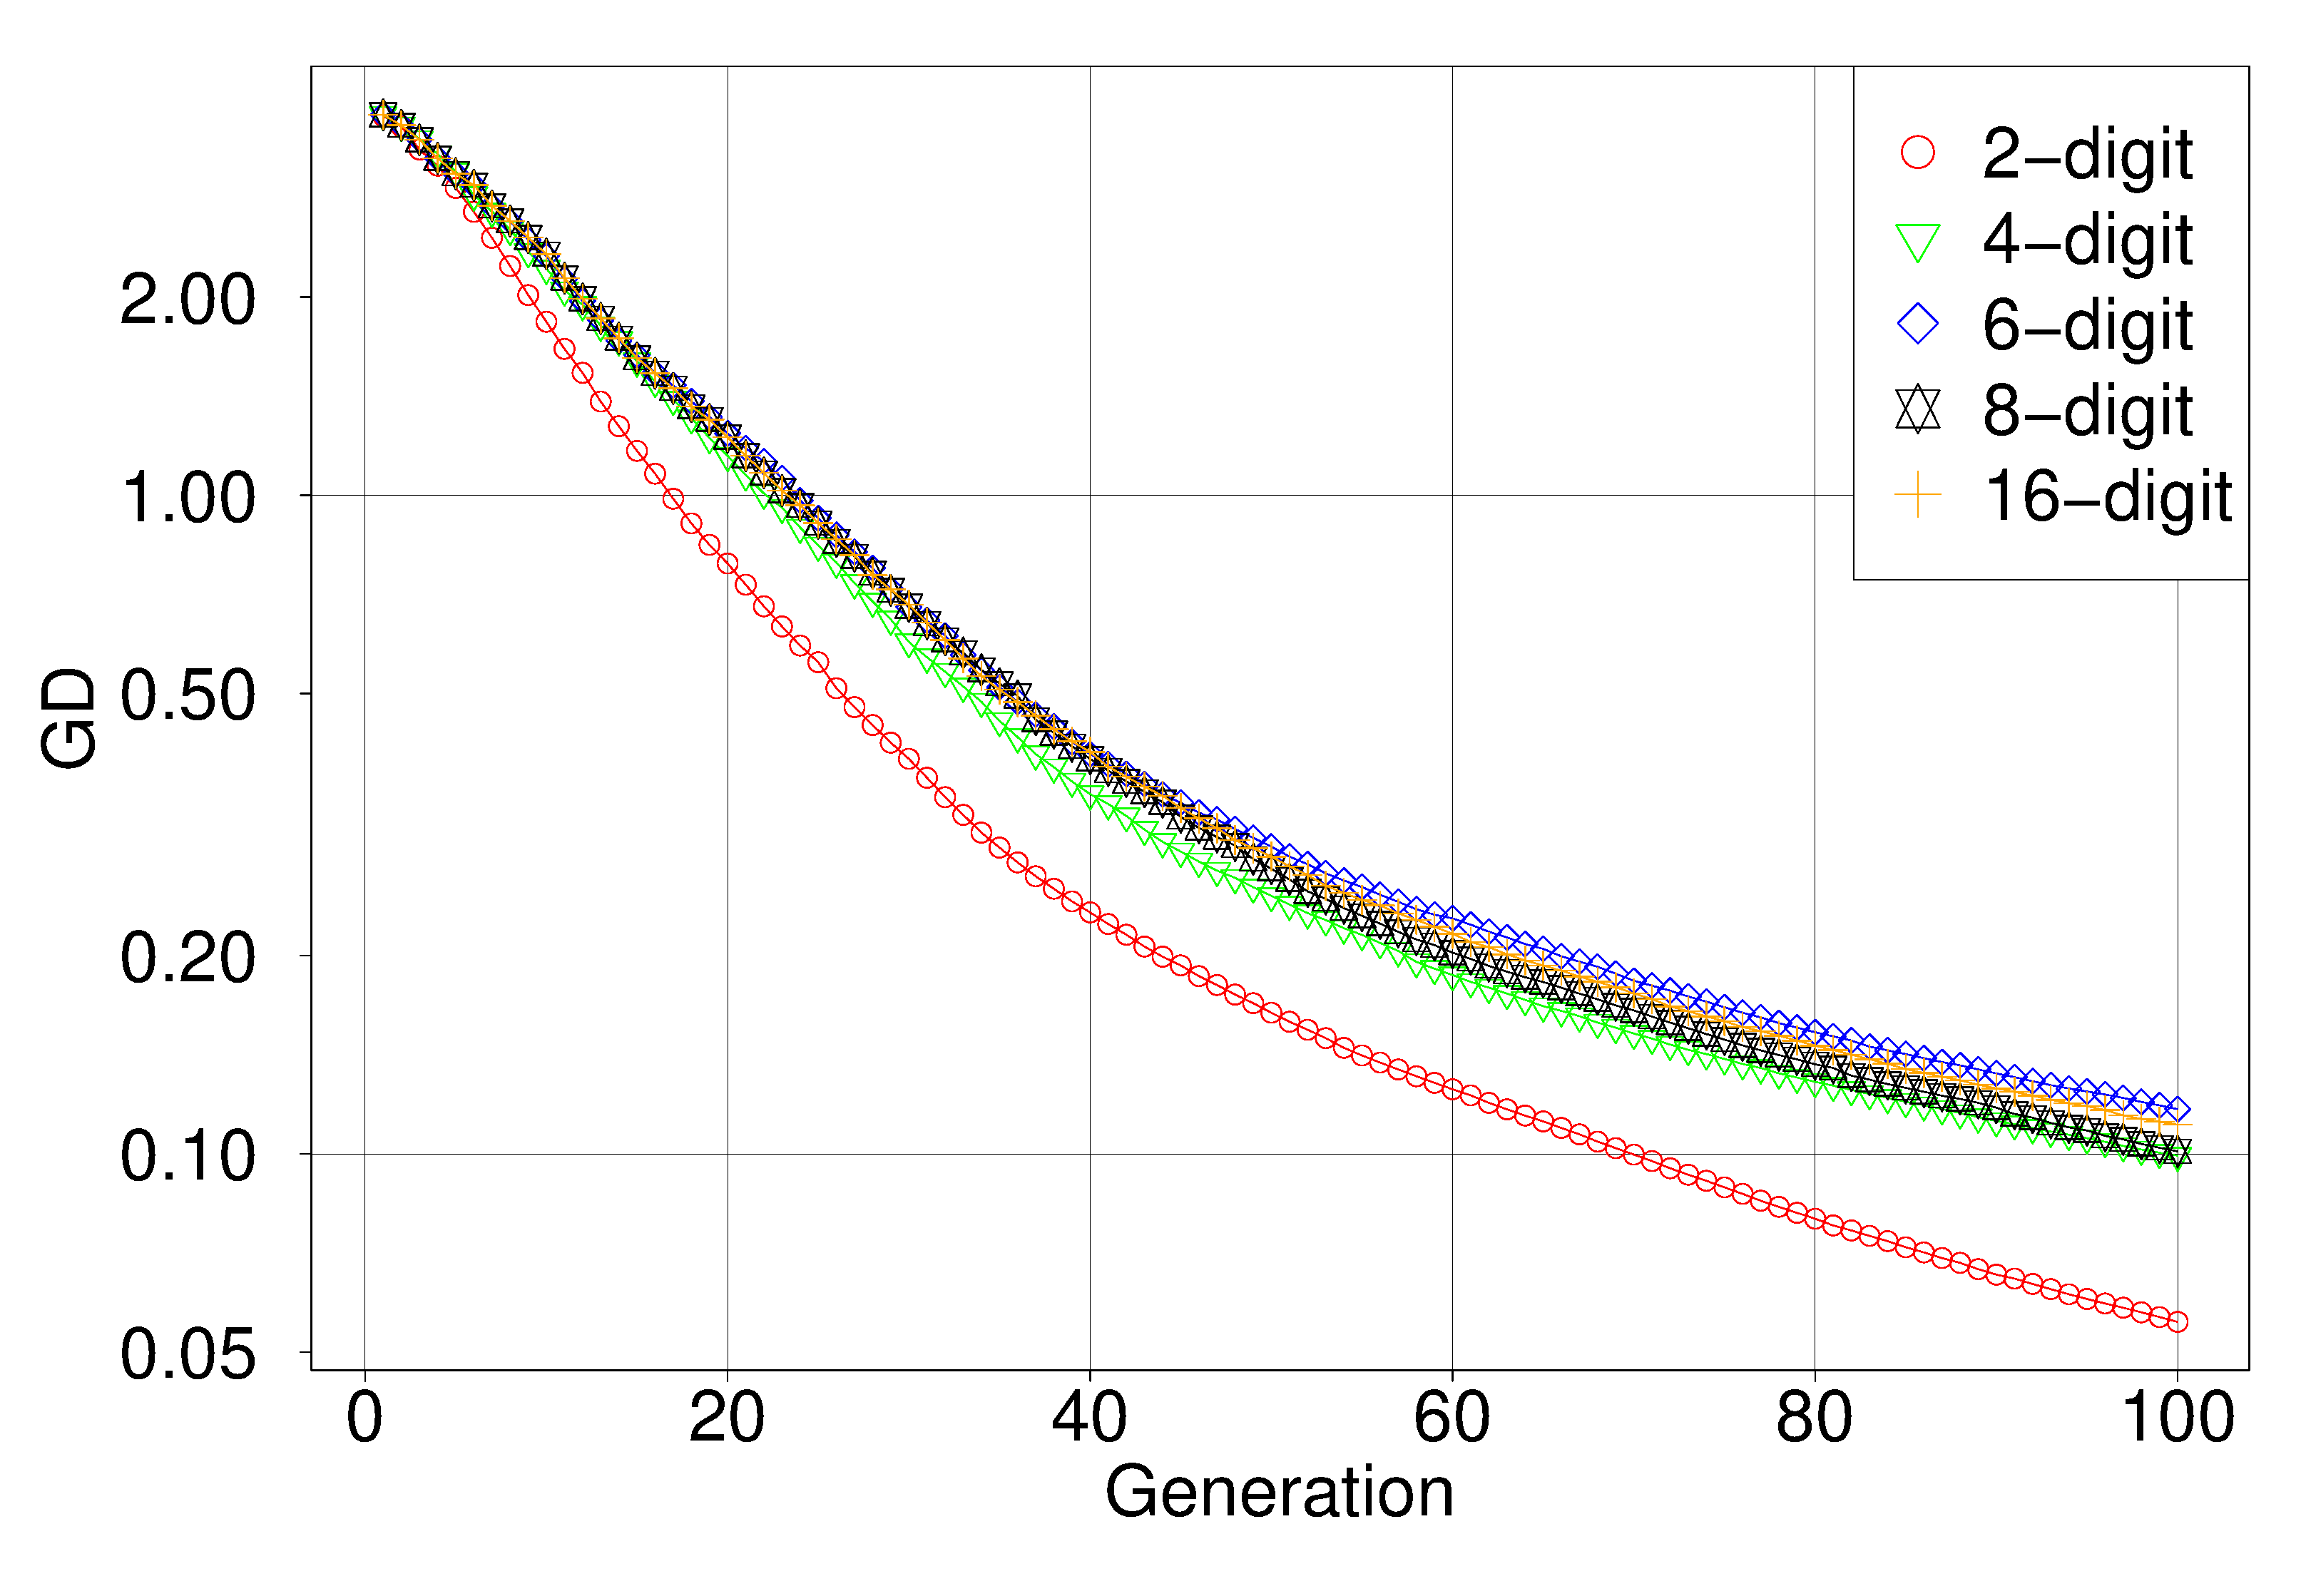
\includegraphics[width=1\linewidth]{../figures/NSGA-II/ano_DTLZ2_GD.eps}
\begin{center}
{\footnotesize (a) Modified DTLZ2}
\end{center}
\end{minipage}
\begin{minipage}{0.32\hsize}
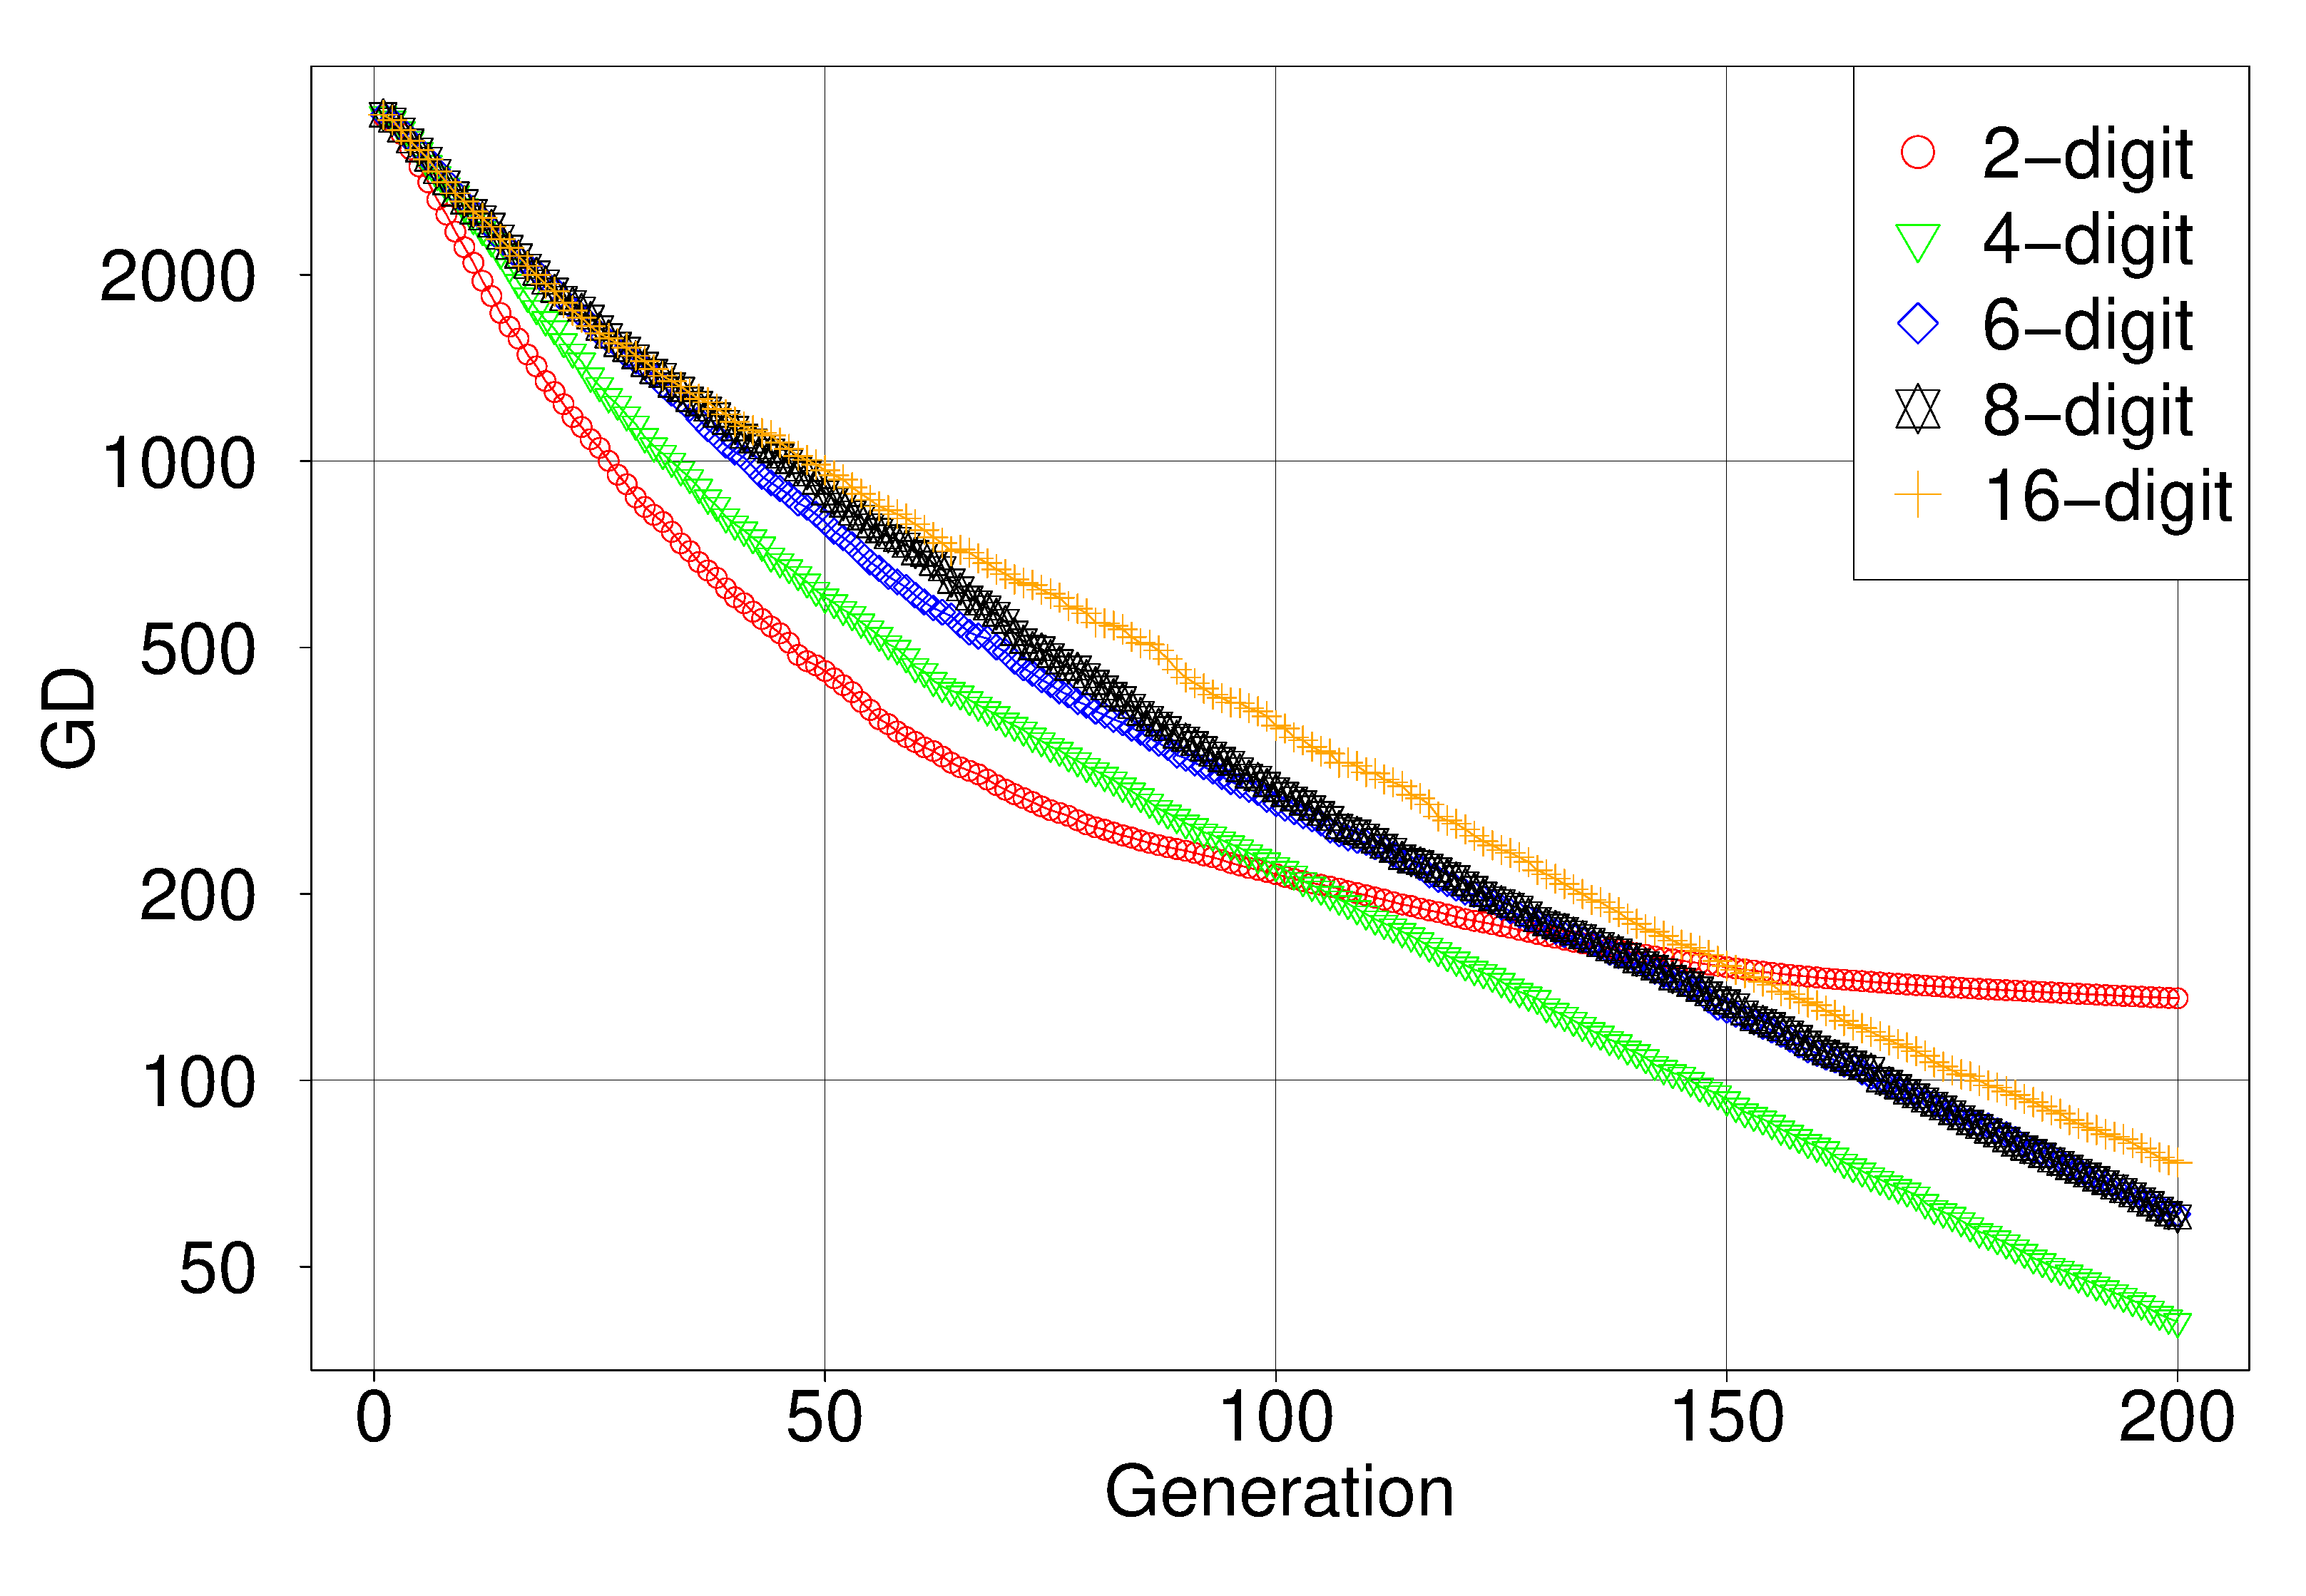
\includegraphics[width=1\linewidth]{../figures/NSGA-II/ano_DTLZ3_GD.eps}
\begin{center}
{\footnotesize (b) Modified DTLZ3}
\end{center}
\end{minipage}
\begin{minipage}{0.32\hsize}
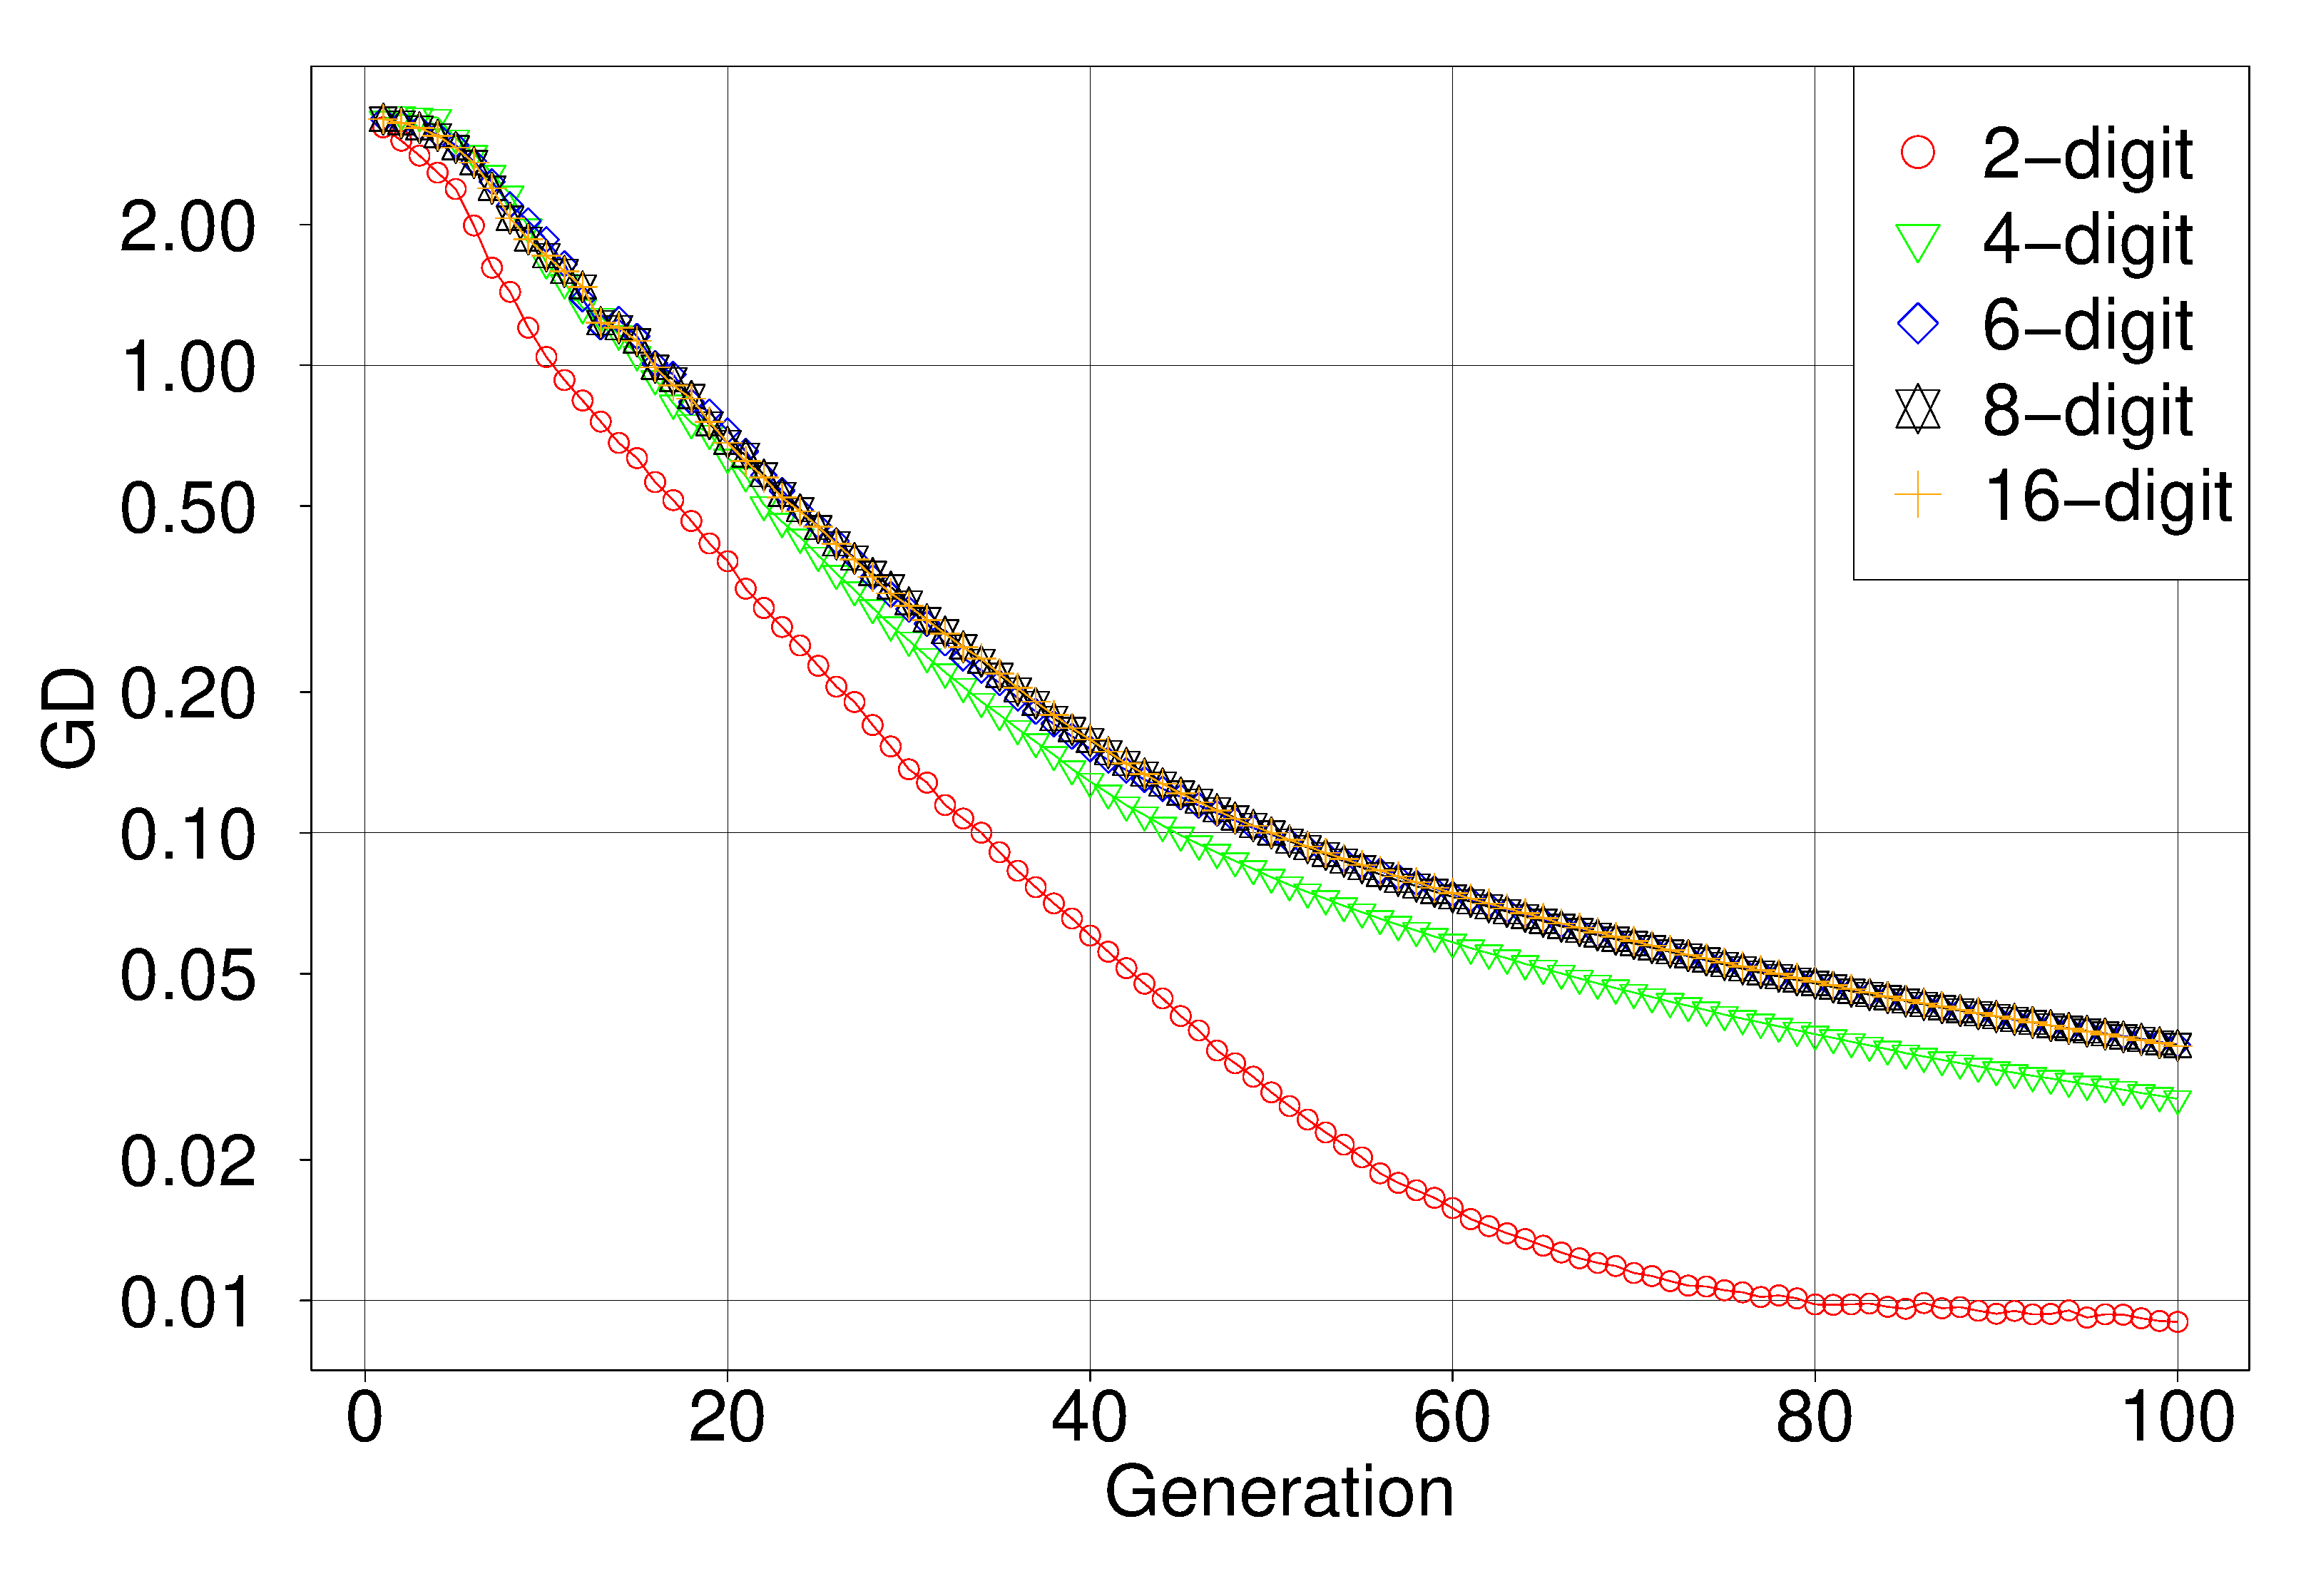
\includegraphics[width=1\linewidth]{../figures/NSGA-II/ano_DTLZ4_GD.eps}
\begin{center}
{\footnotesize (c) Modified DTLZ4}
\end{center}
\end{minipage}
\end{tabular}
\caption{Modified DTLZ2-4におけるGDの推移(NSGA-II)}
\label{fig:gd_mod_nsgaii}
\end{figure*}


\begin{figure*}[htbp]
\begin{tabular}{cc}
\begin{minipage}{0.32\hsize}
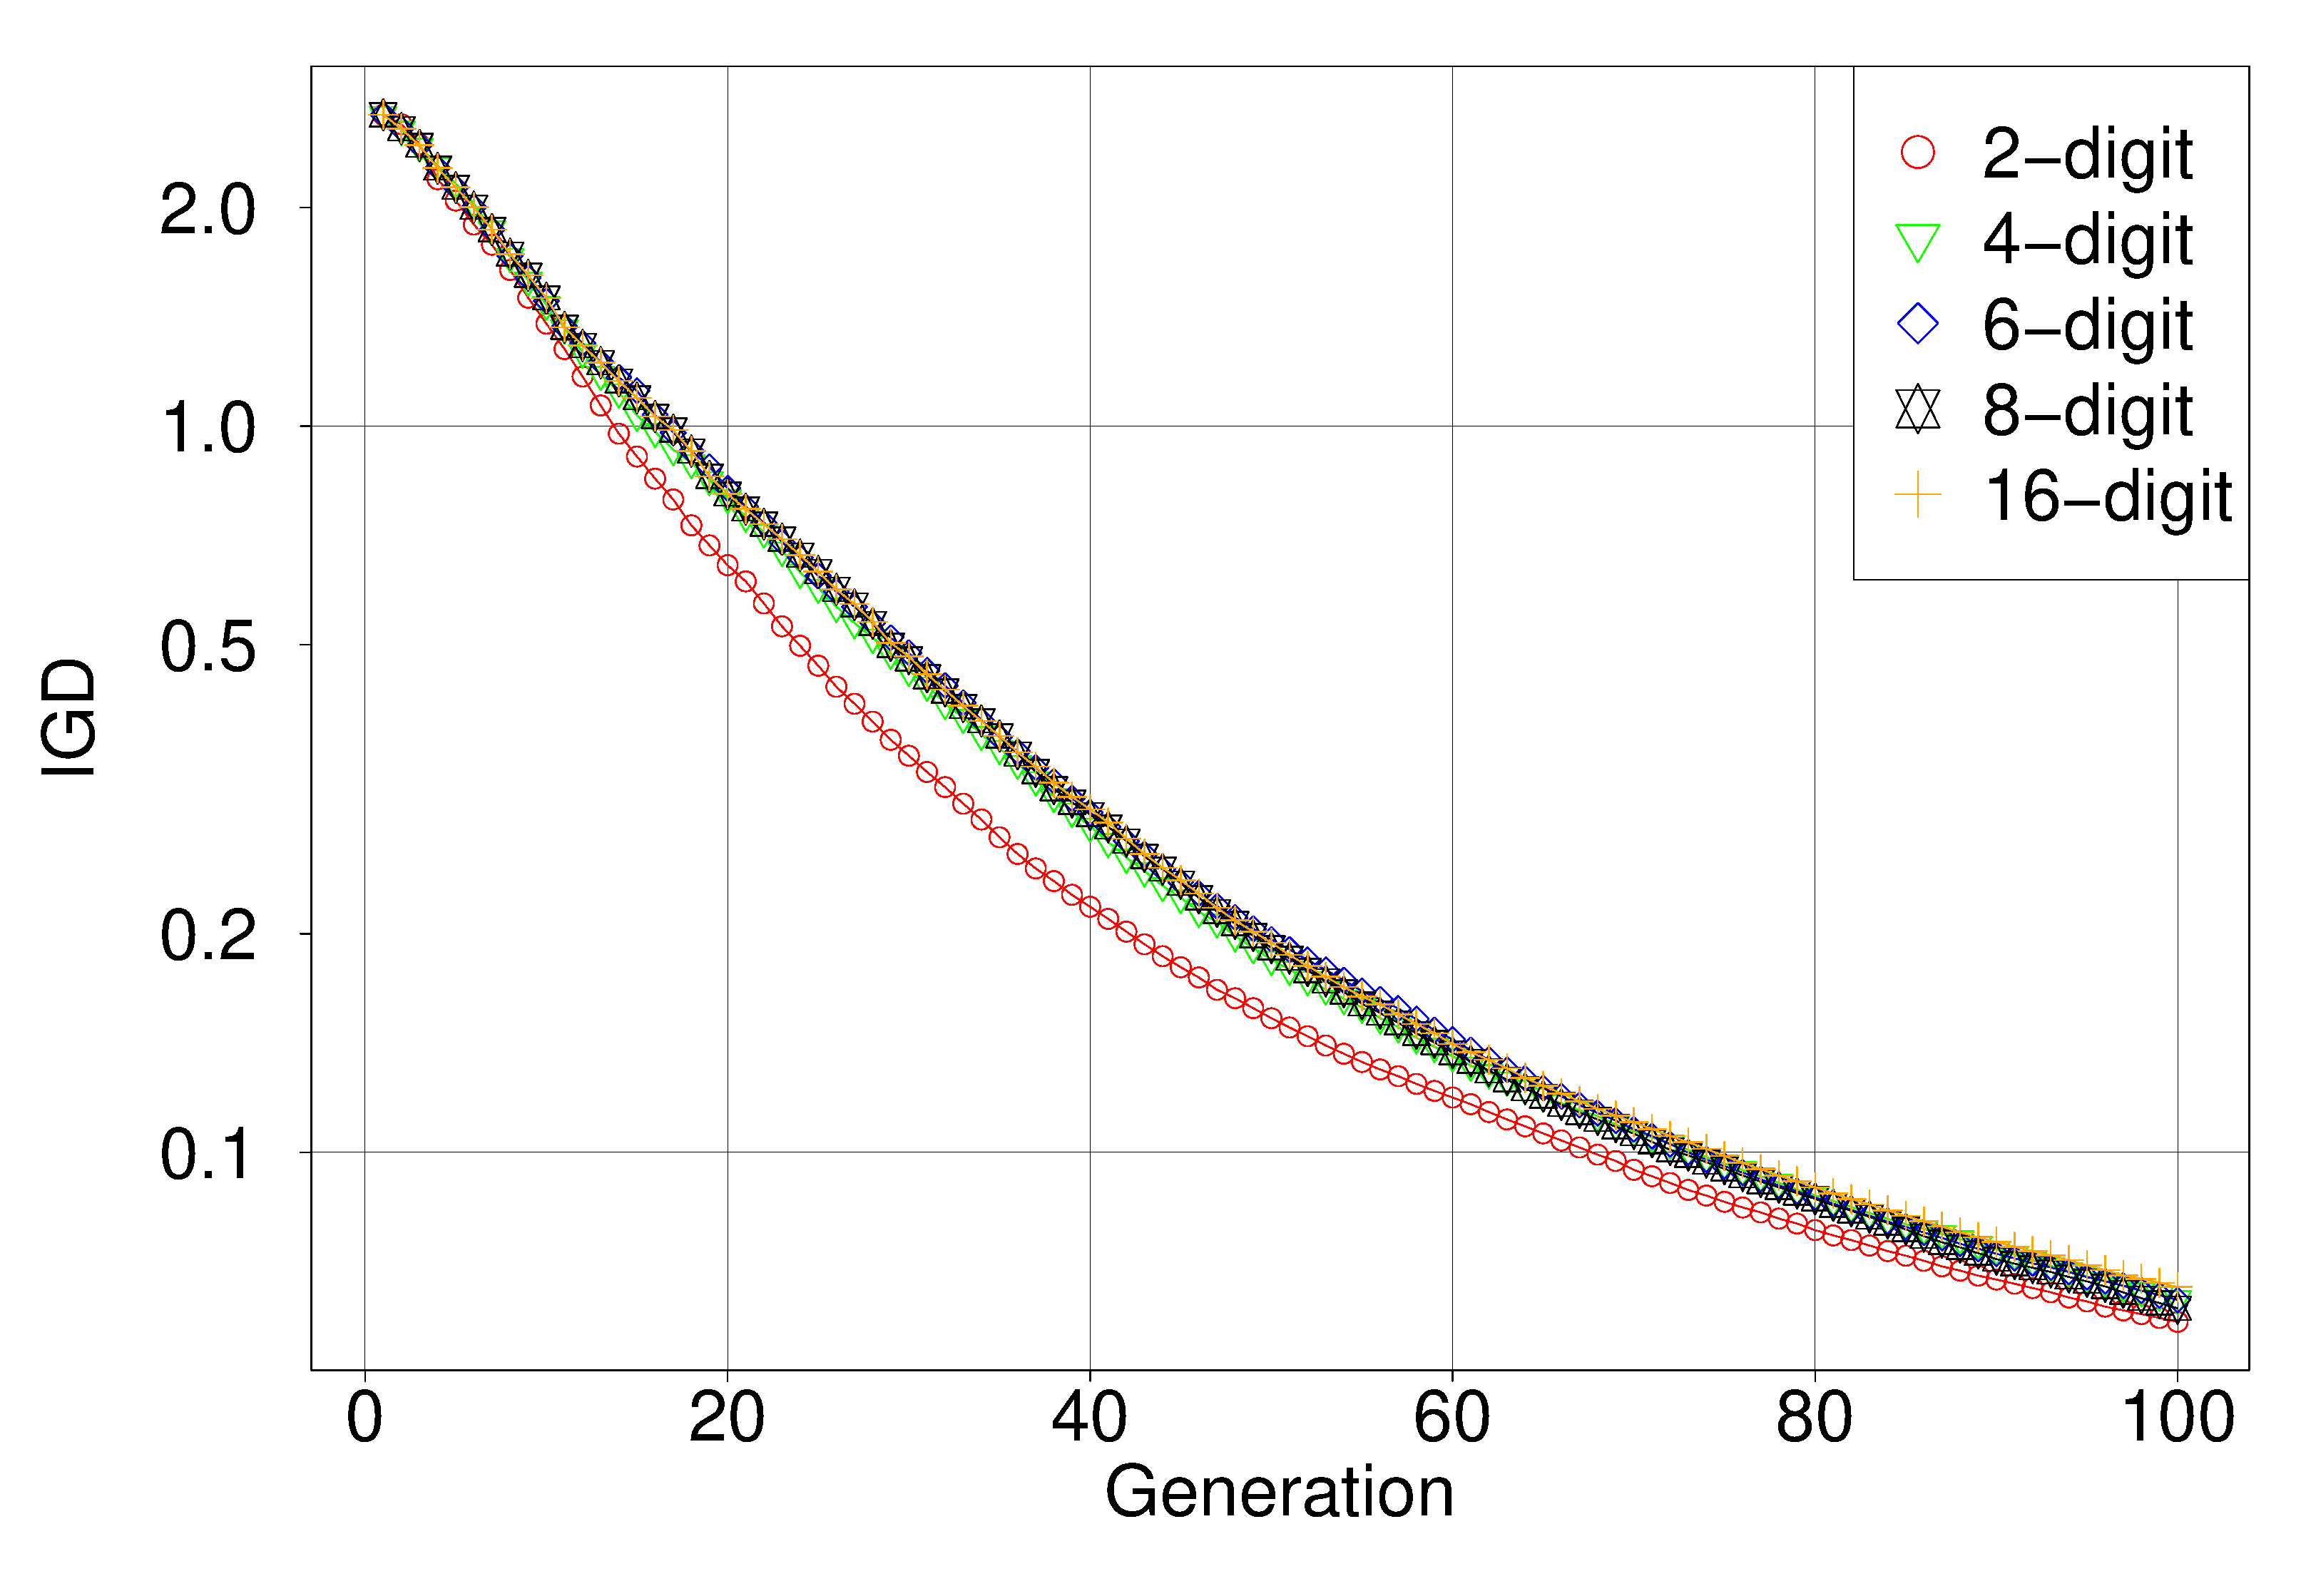
\includegraphics[width=1\linewidth]{../figures/NSGA-II/ano_DTLZ2_IGD.eps}
\begin{center}
{\footnotesize (a) Modified DTLZ2}
\end{center}
\end{minipage}
\begin{minipage}{0.32\hsize}
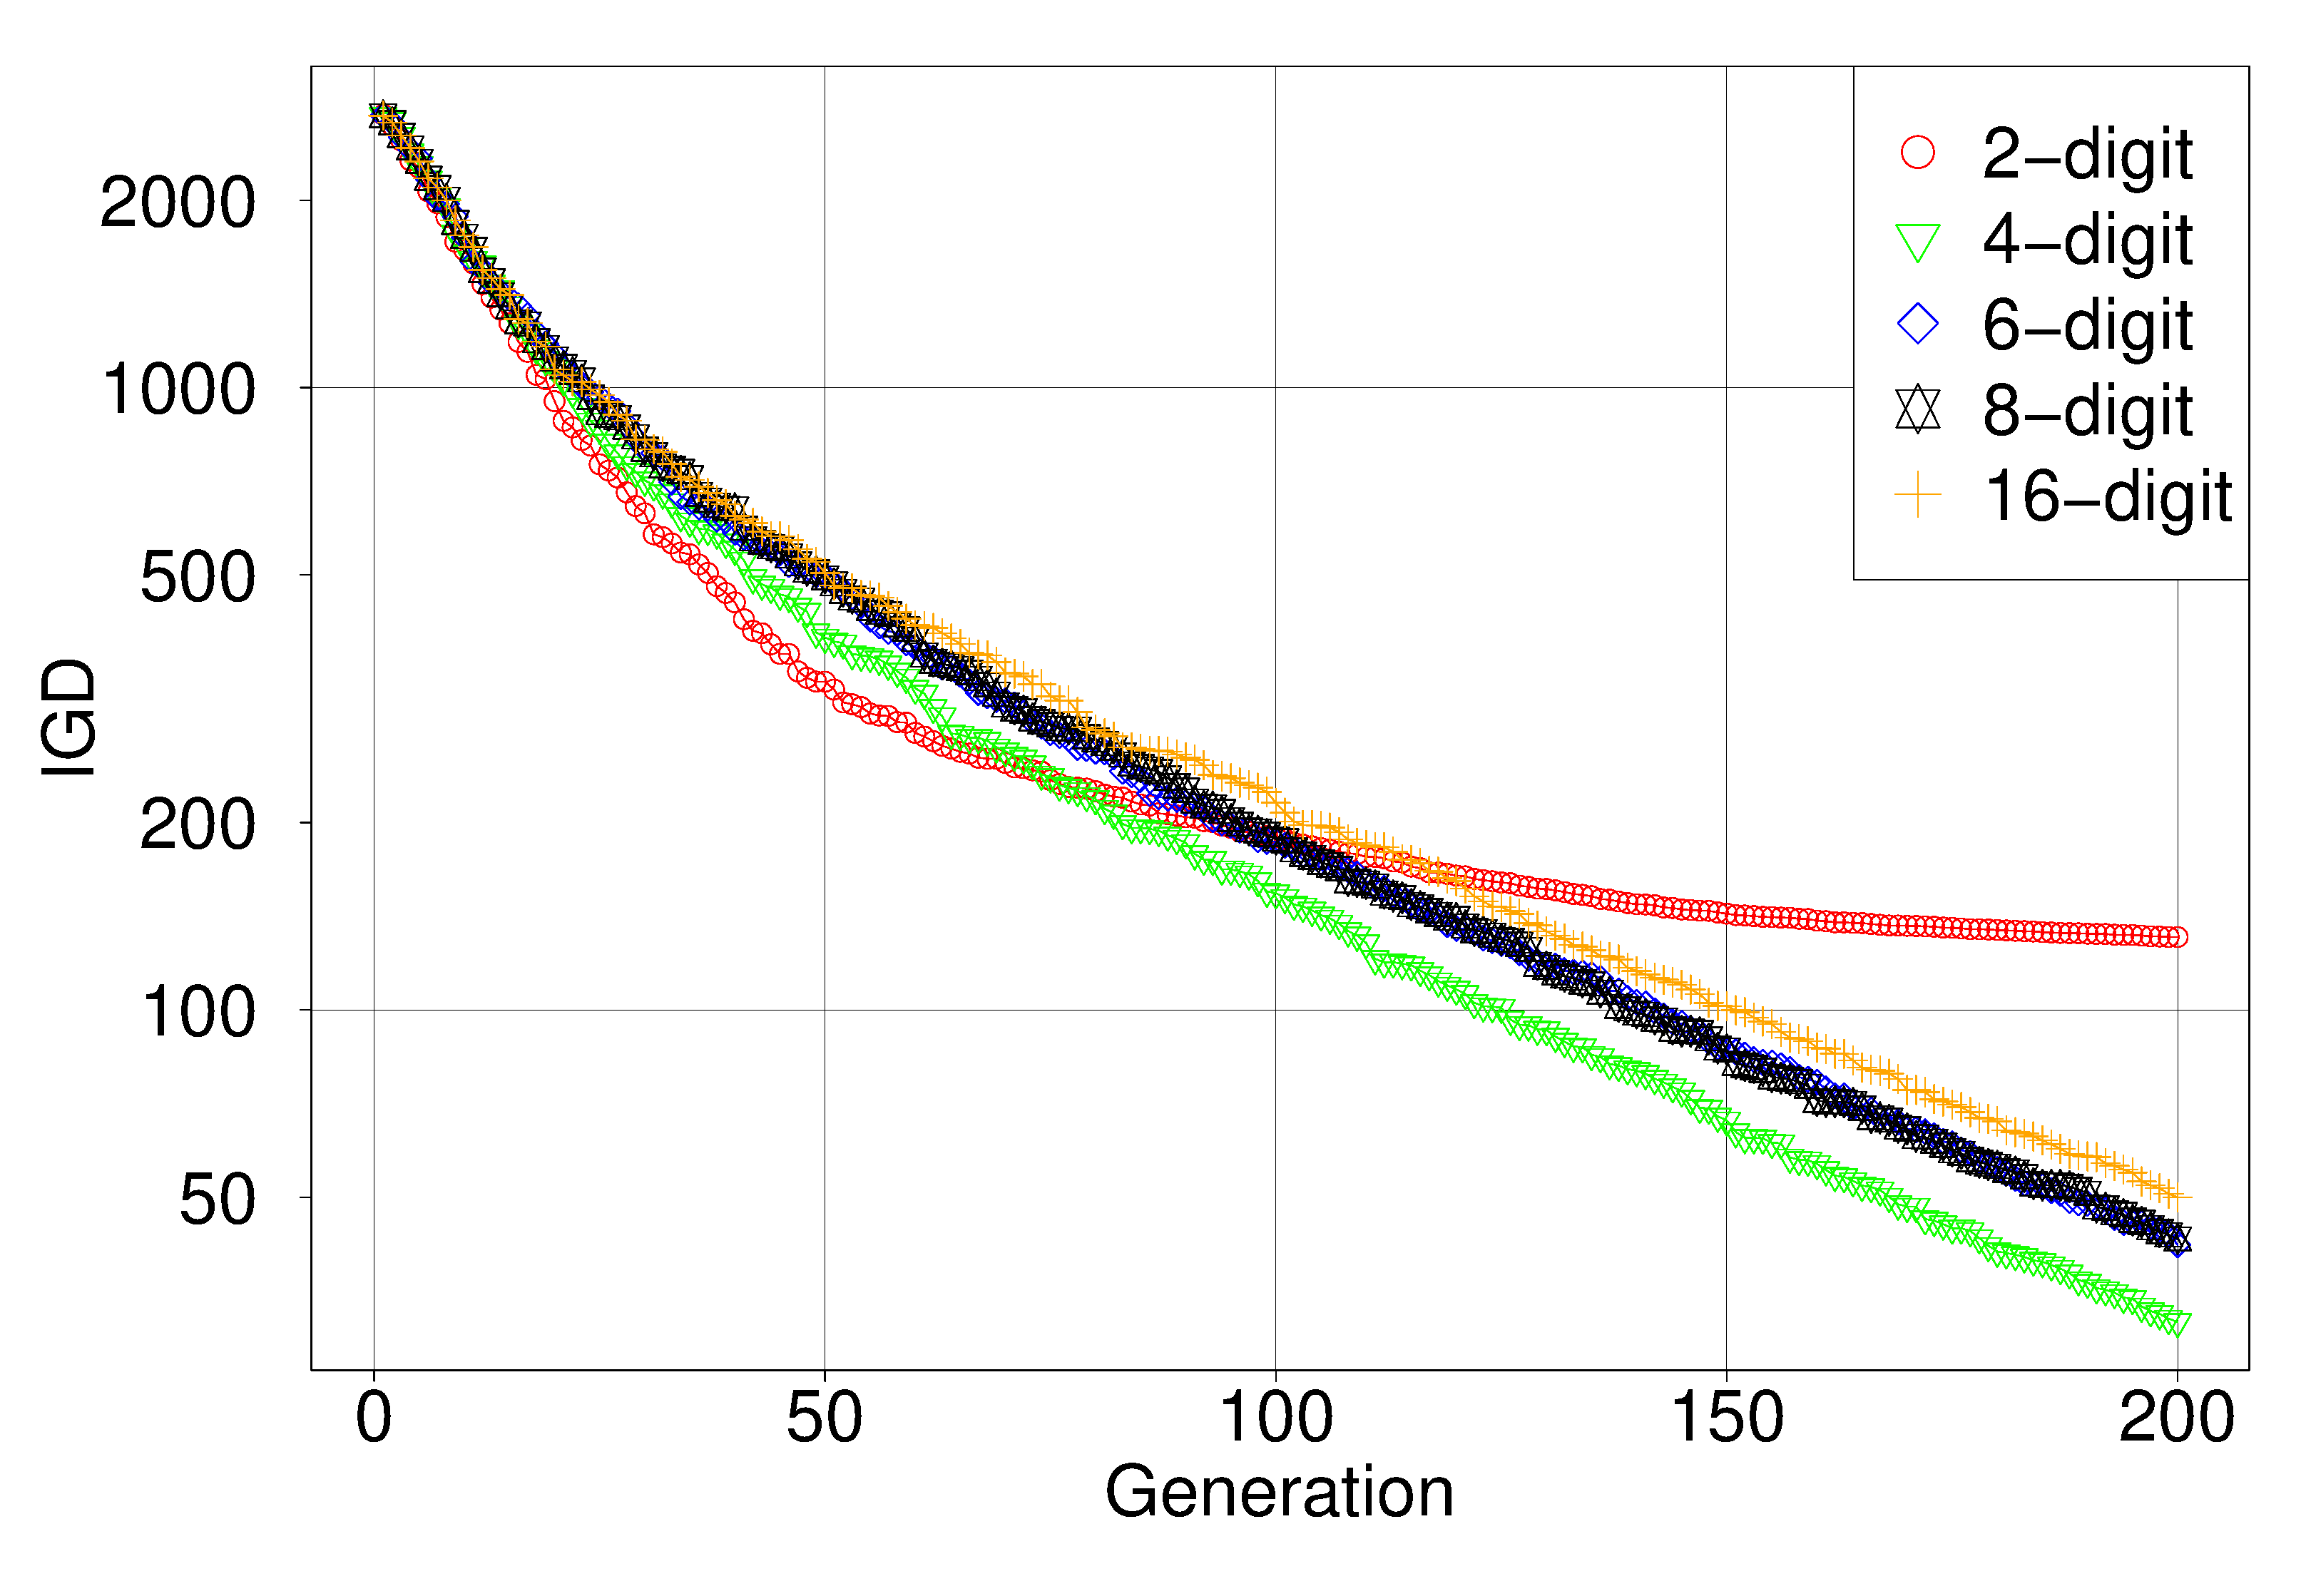
\includegraphics[width=1\linewidth]{../figures/NSGA-II/ano_DTLZ3_IGD.eps}
\begin{center}
{\footnotesize (b) Modified DTLZ3}
\end{center}
\end{minipage}
\begin{minipage}{0.32\hsize}
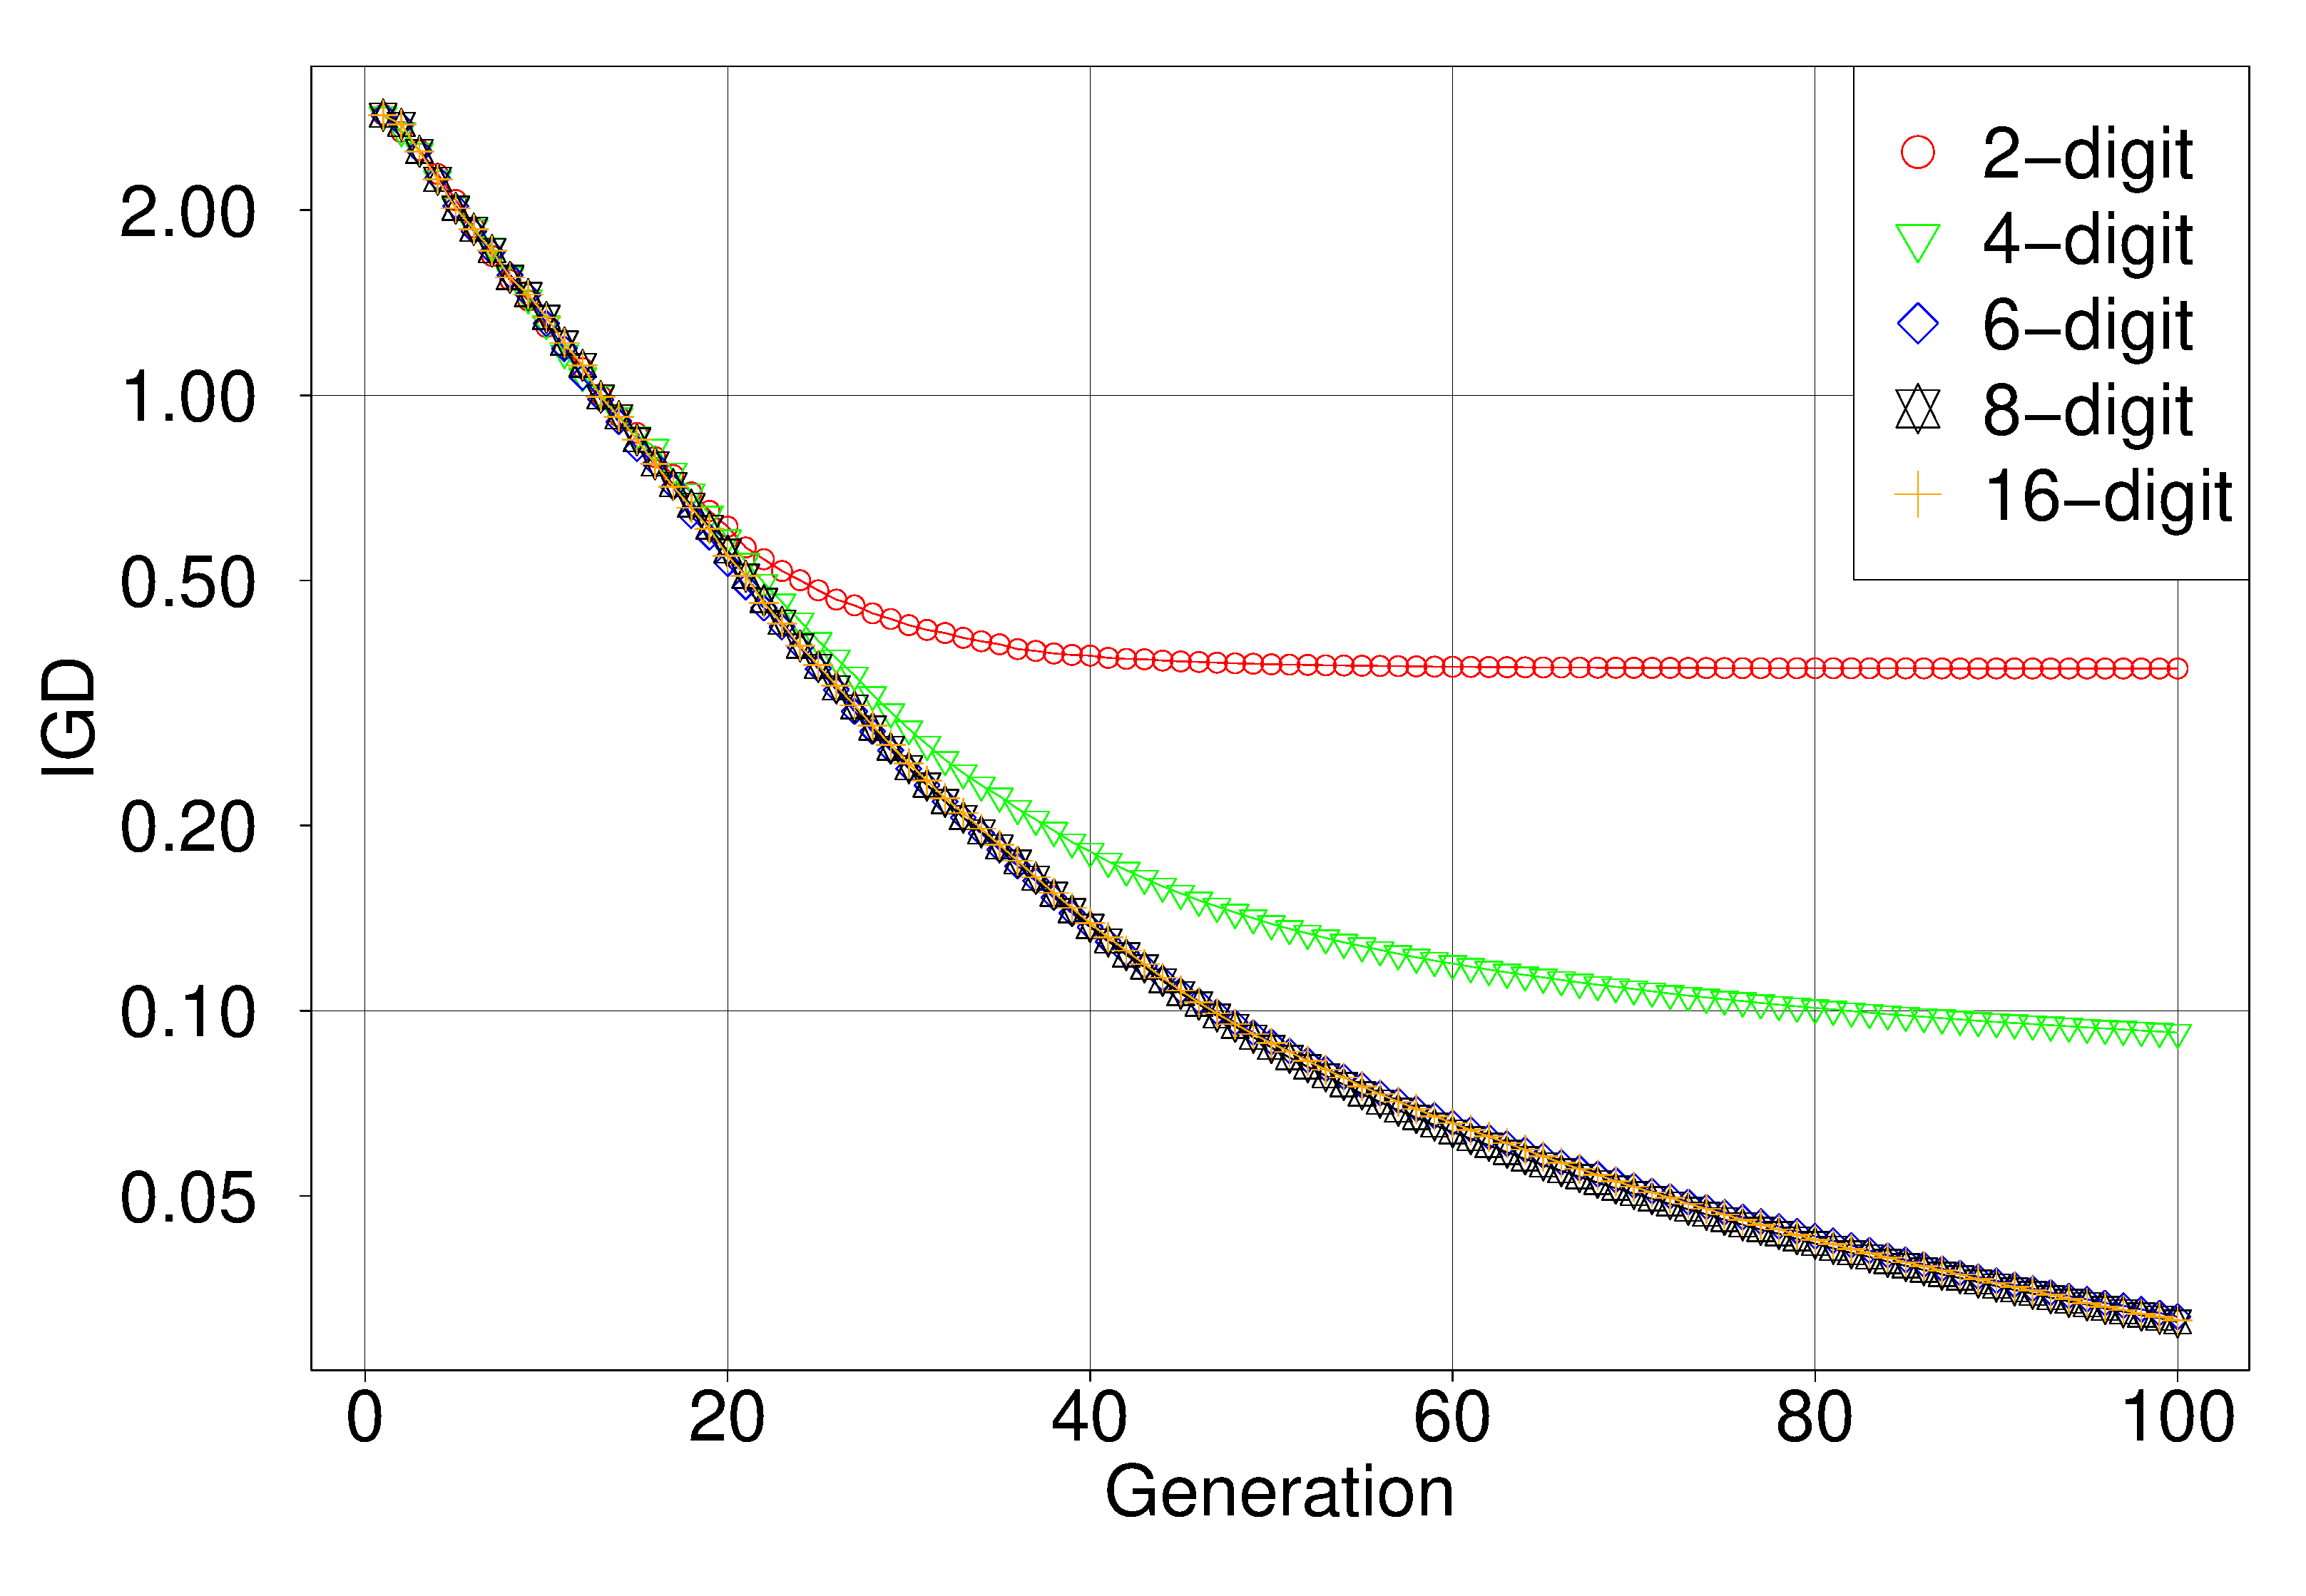
\includegraphics[width=1\linewidth]{../figures/NSGA-II/ano_DTLZ4_IGD.eps}
\begin{center}
{\footnotesize (c) Modified DTLZ4}
\end{center}
\end{minipage}
\end{tabular}
\caption{Modified DTLZ2-4におけるIGDの推移(NSGA-II)}
\label{fig:igd_mod_nsgaii}
\end{figure*}

\begin{figure*}[htbp]
\begin{tabular}{cc}
\begin{minipage}{0.32\hsize}
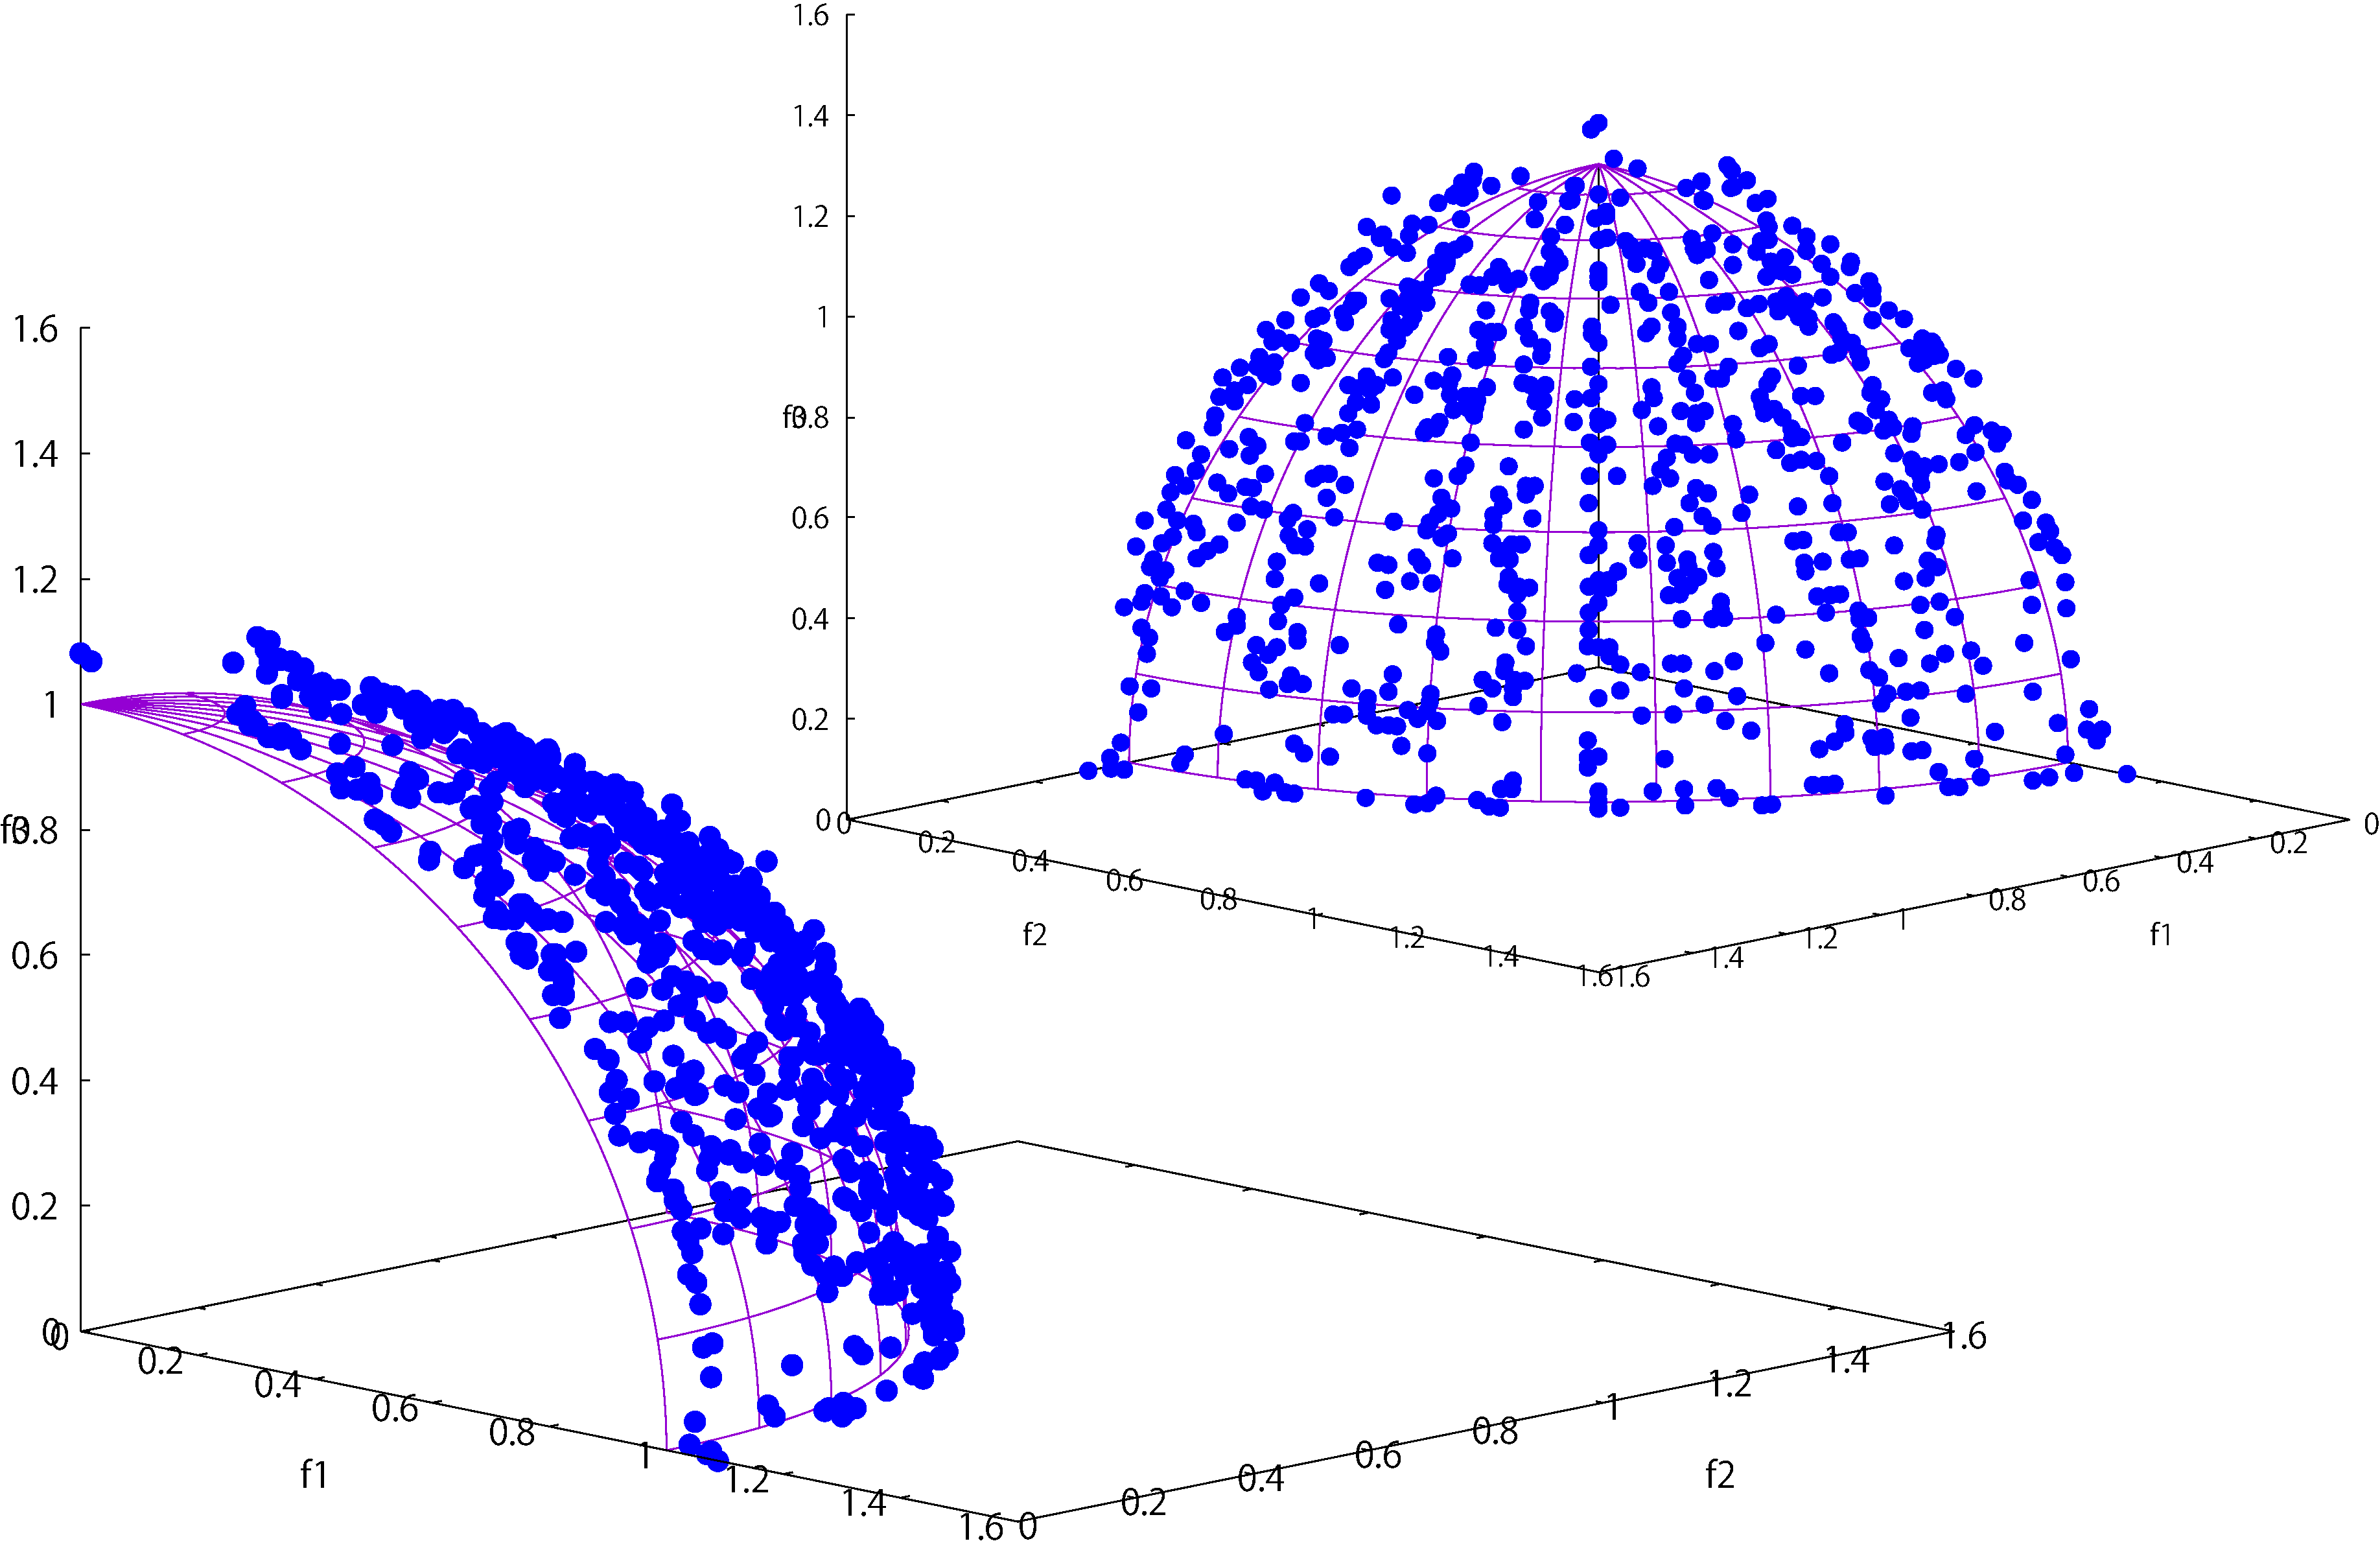
\includegraphics[width=1\linewidth]{../figures/NSGA-II/modDTLZ2_digi2_double.pdf}
\begin{center}
{\footnotesize (a) 2桁}
\end{center}
\end{minipage}
\begin{minipage}{0.32\hsize}
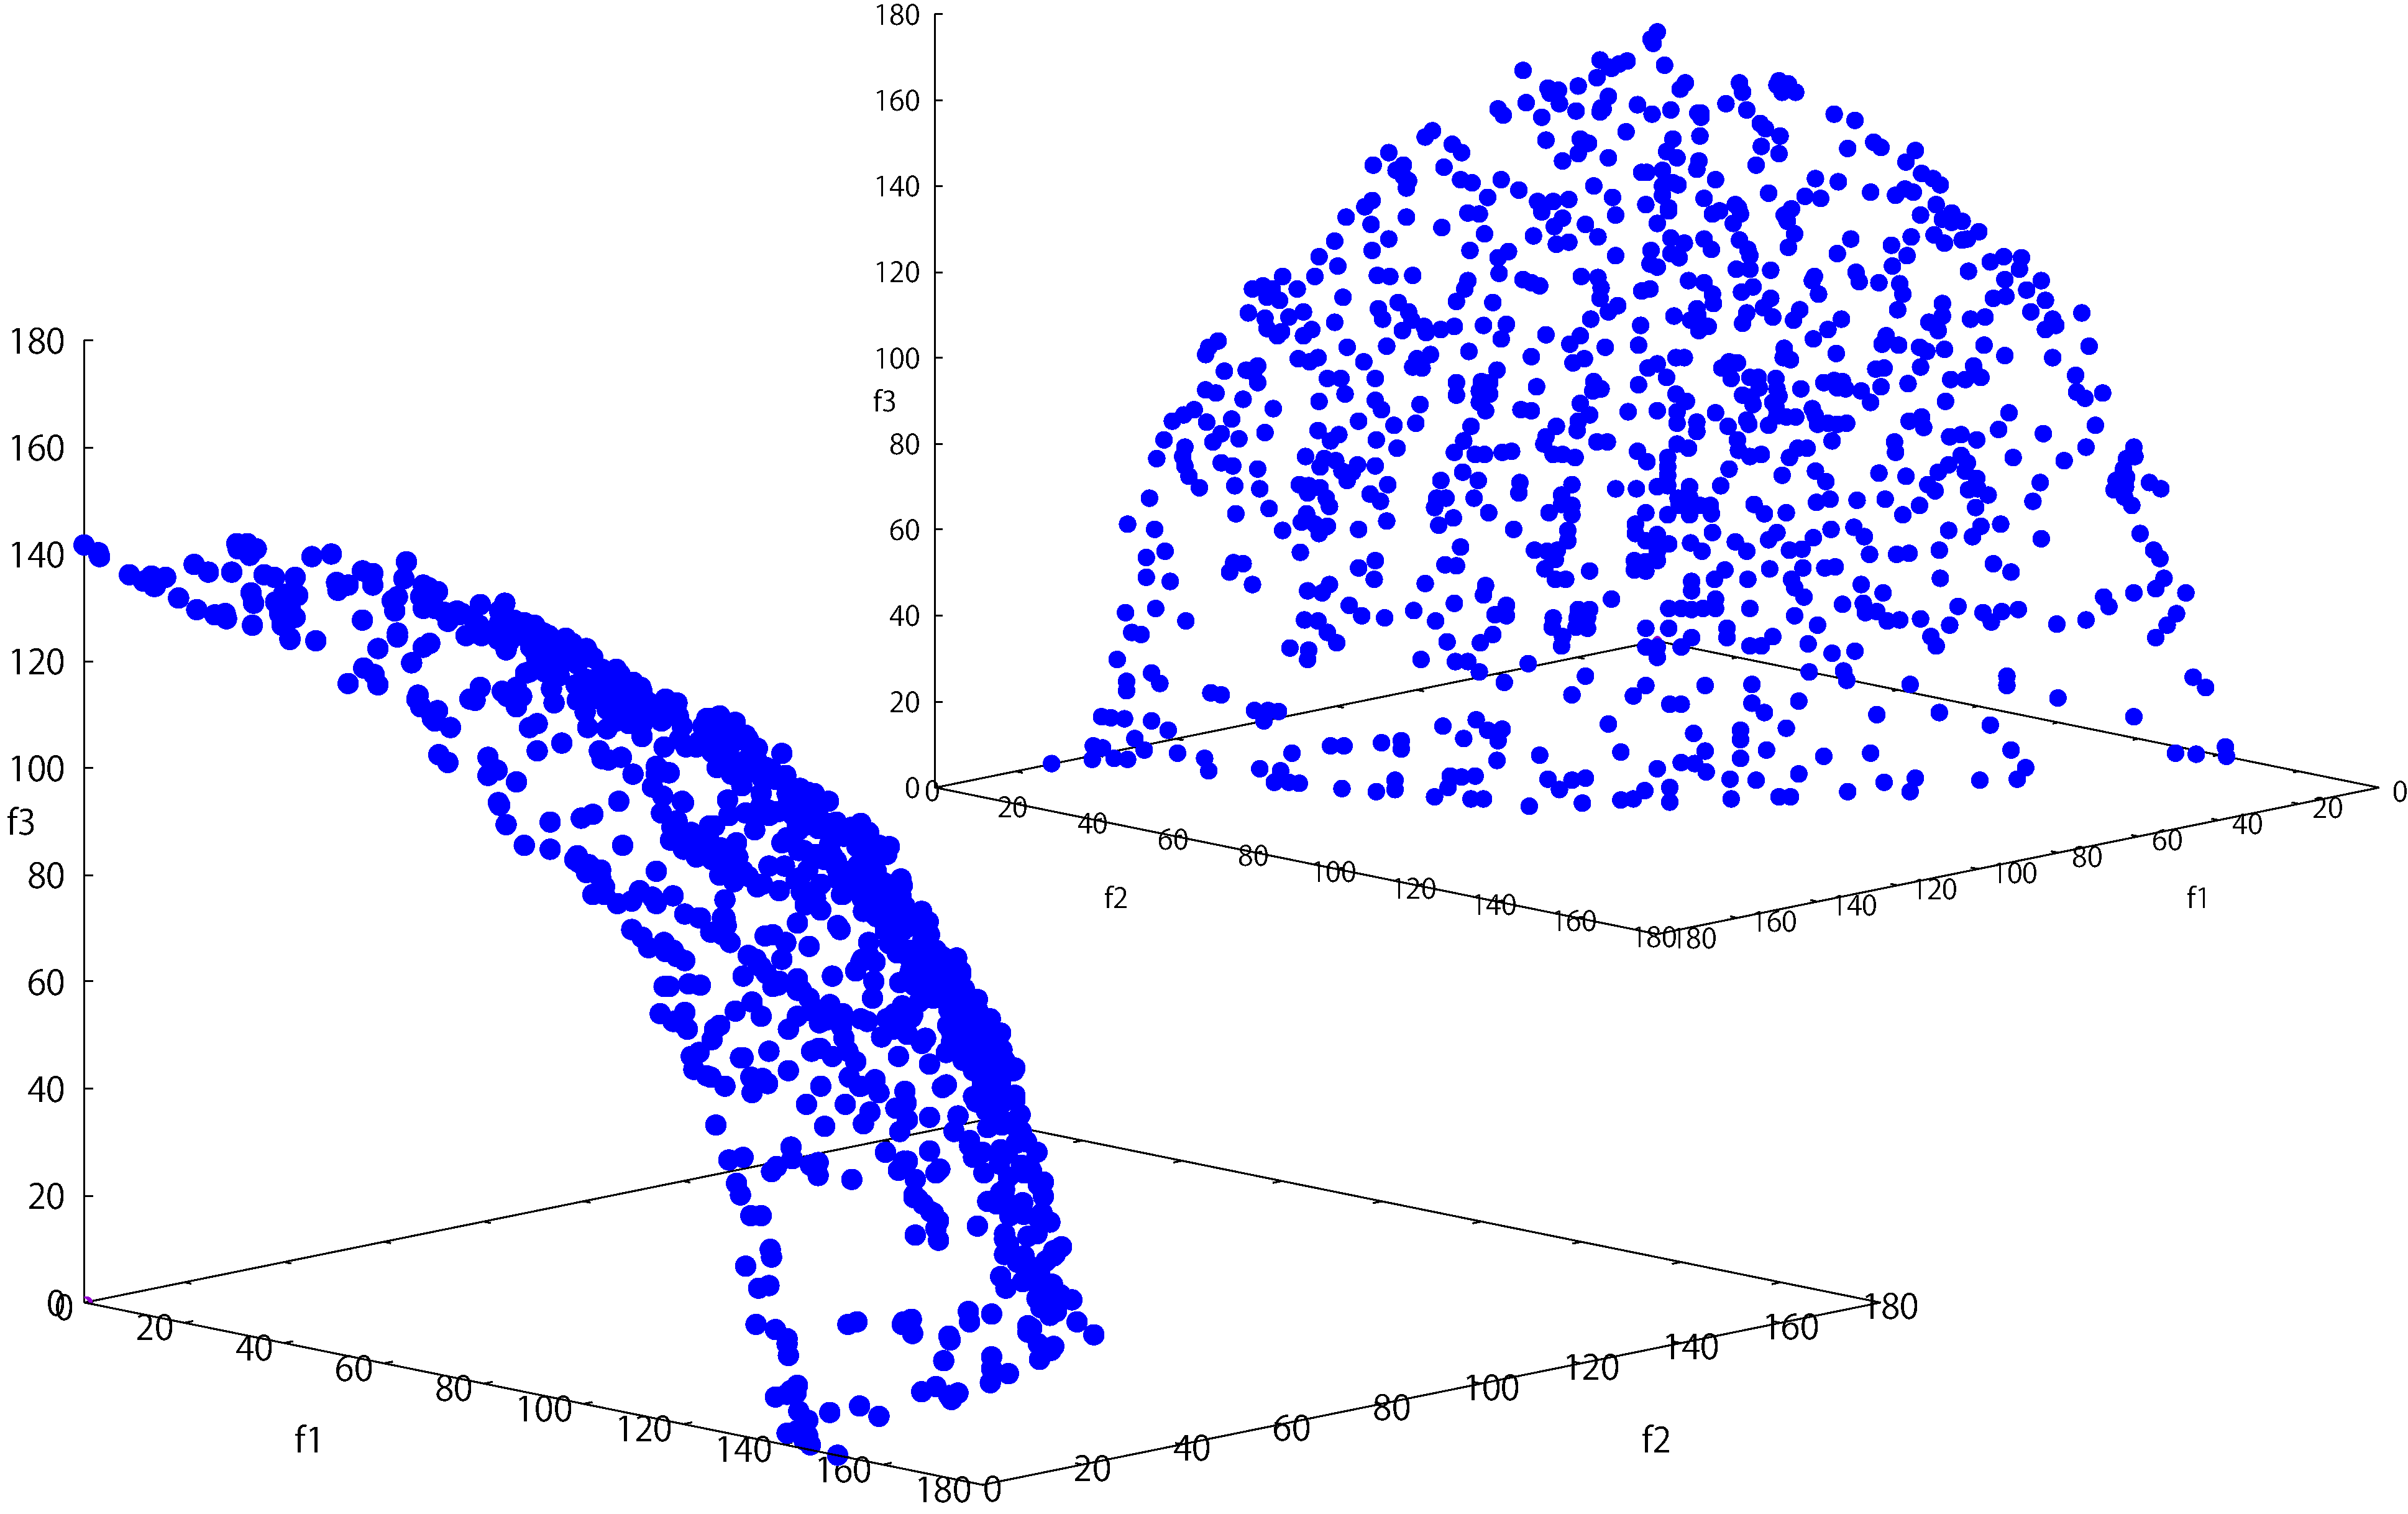
\includegraphics[width=1\linewidth]{../figures/NSGA-II/modDTLZ3_digi2_double.pdf}
\begin{center}
{\footnotesize (a) 2桁}
\end{center}
\end{minipage}
\begin{minipage}{0.32\hsize}
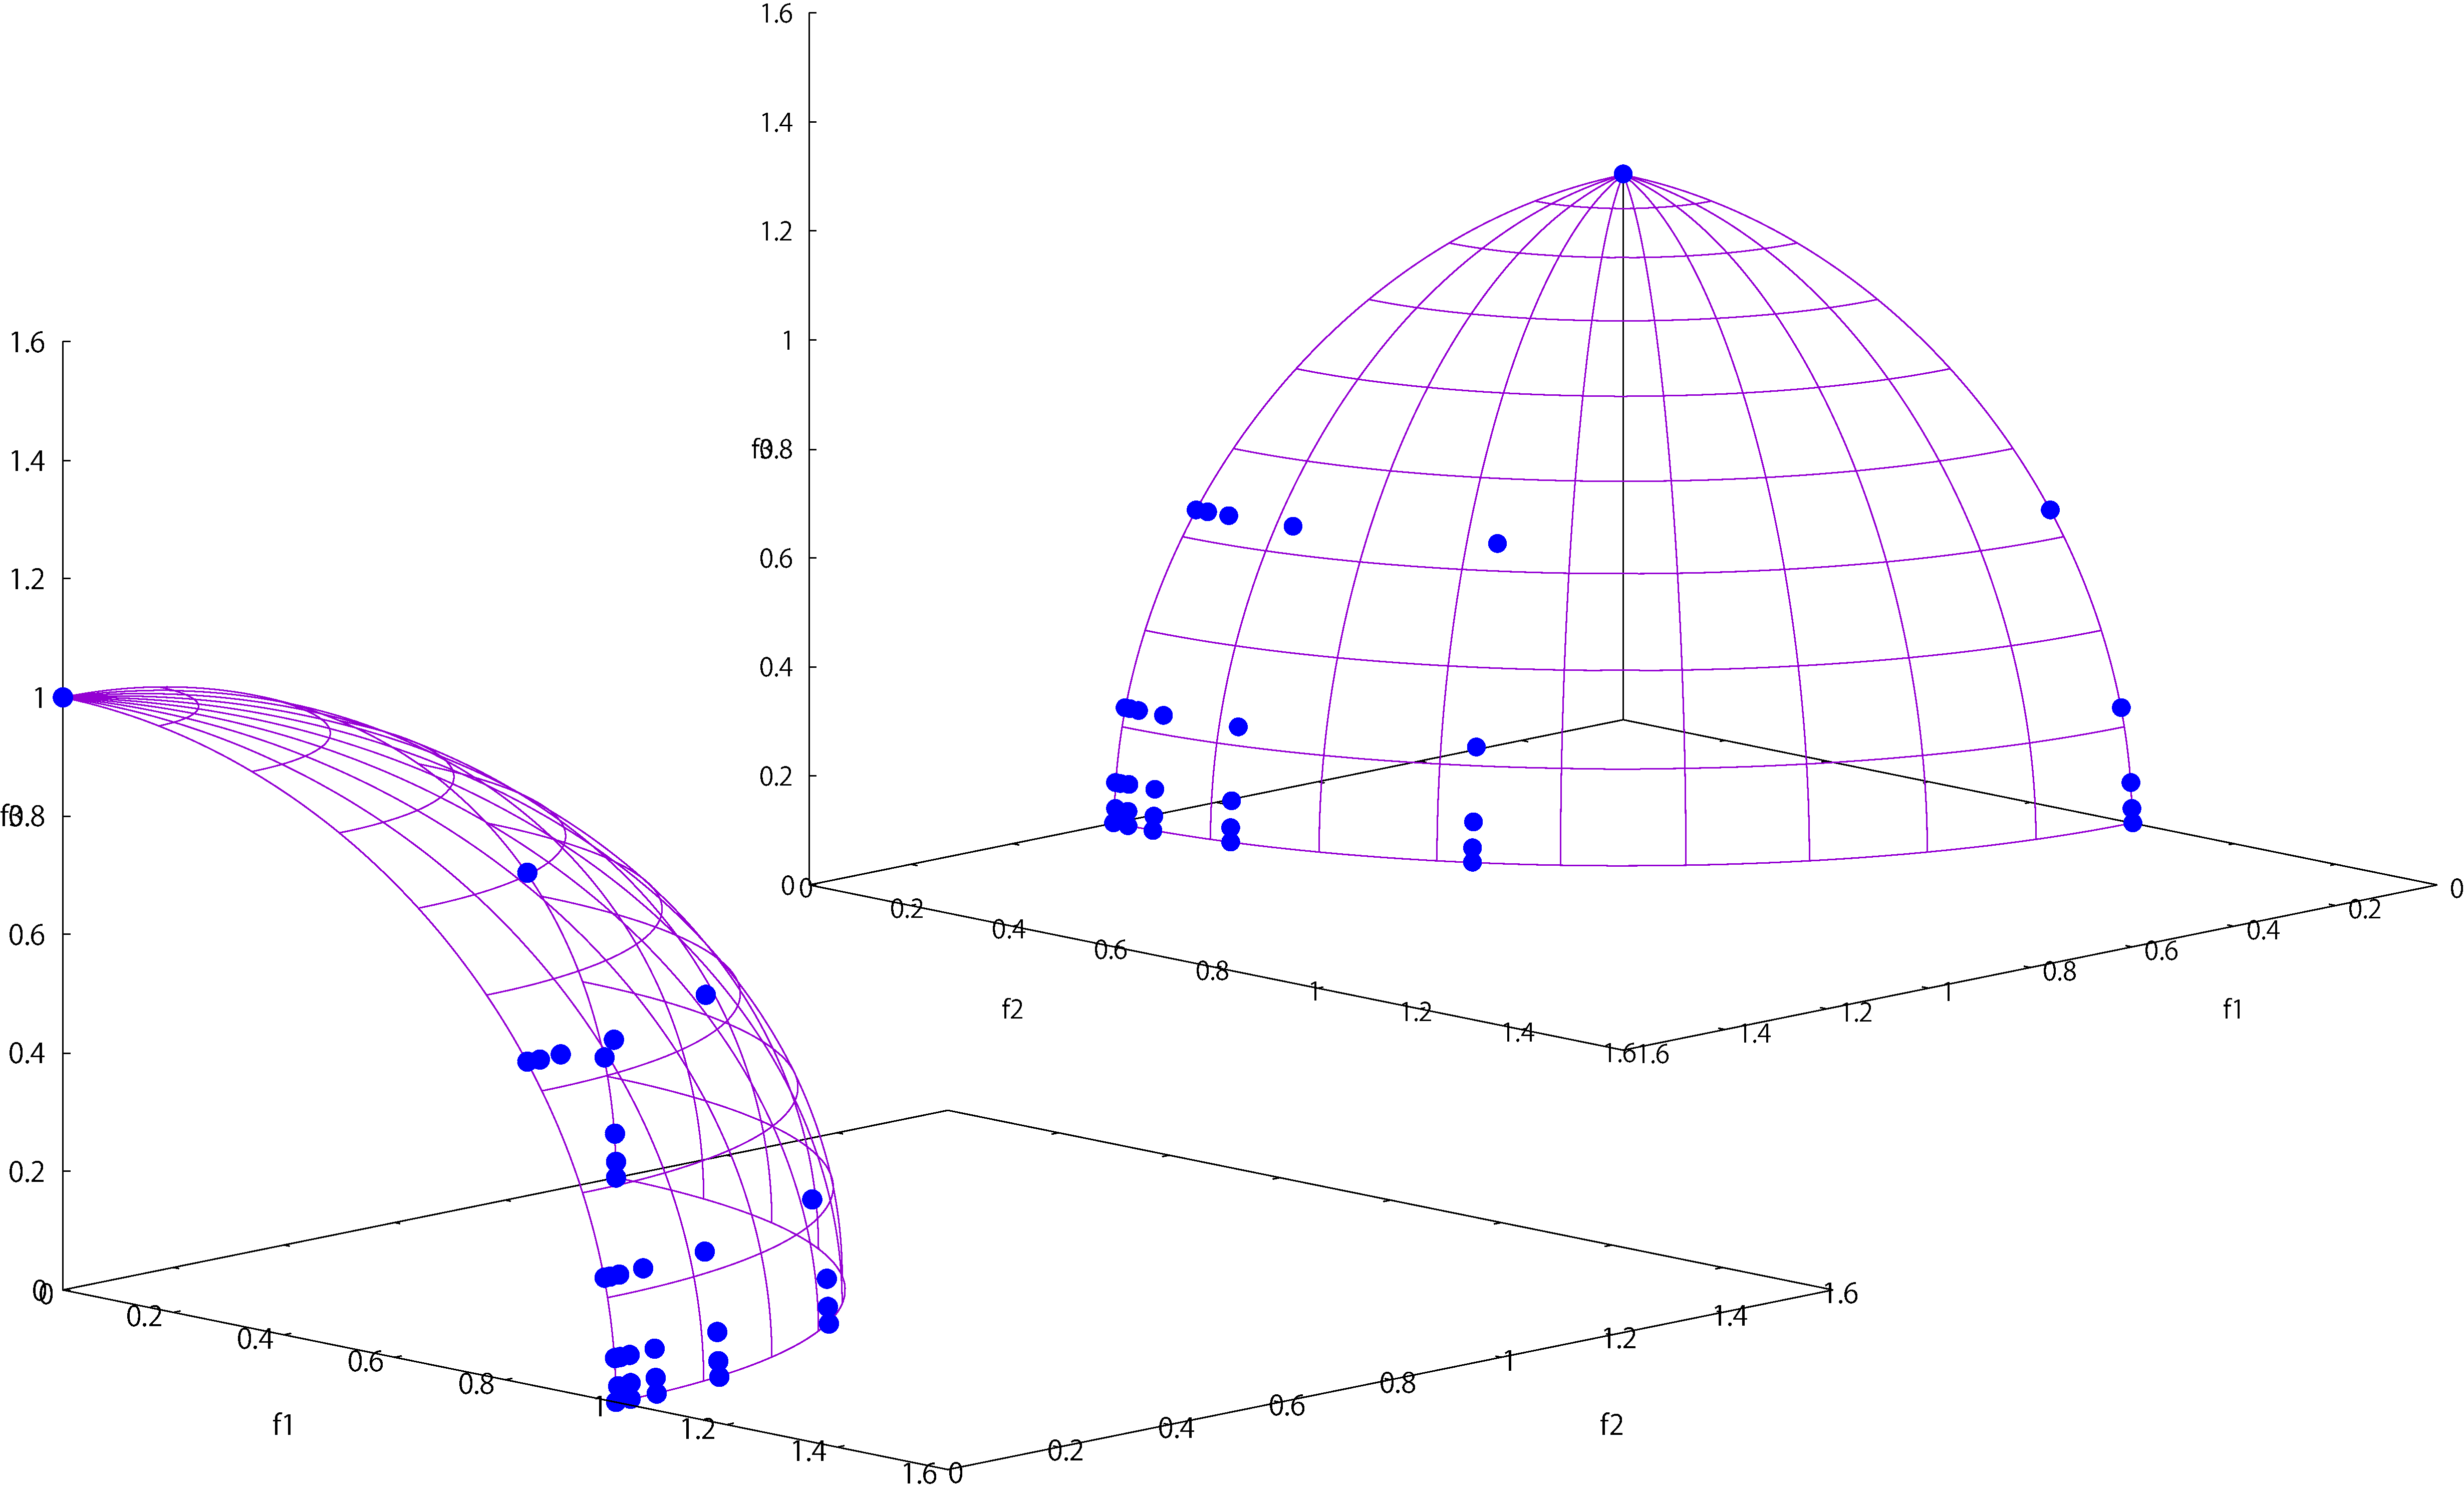
\includegraphics[width=1\linewidth]{../figures/NSGA-II/ano_DTLZ4_digi2_double.pdf}
\begin{center}
{\footnotesize (a) 2桁}
\end{center}
\end{minipage}
\end{tabular}
%\label{fig:dtlz4}
\end{figure*}

\begin{figure*}[!h]
\begin{tabular}{cc}
\begin{minipage}{0.32\hsize}
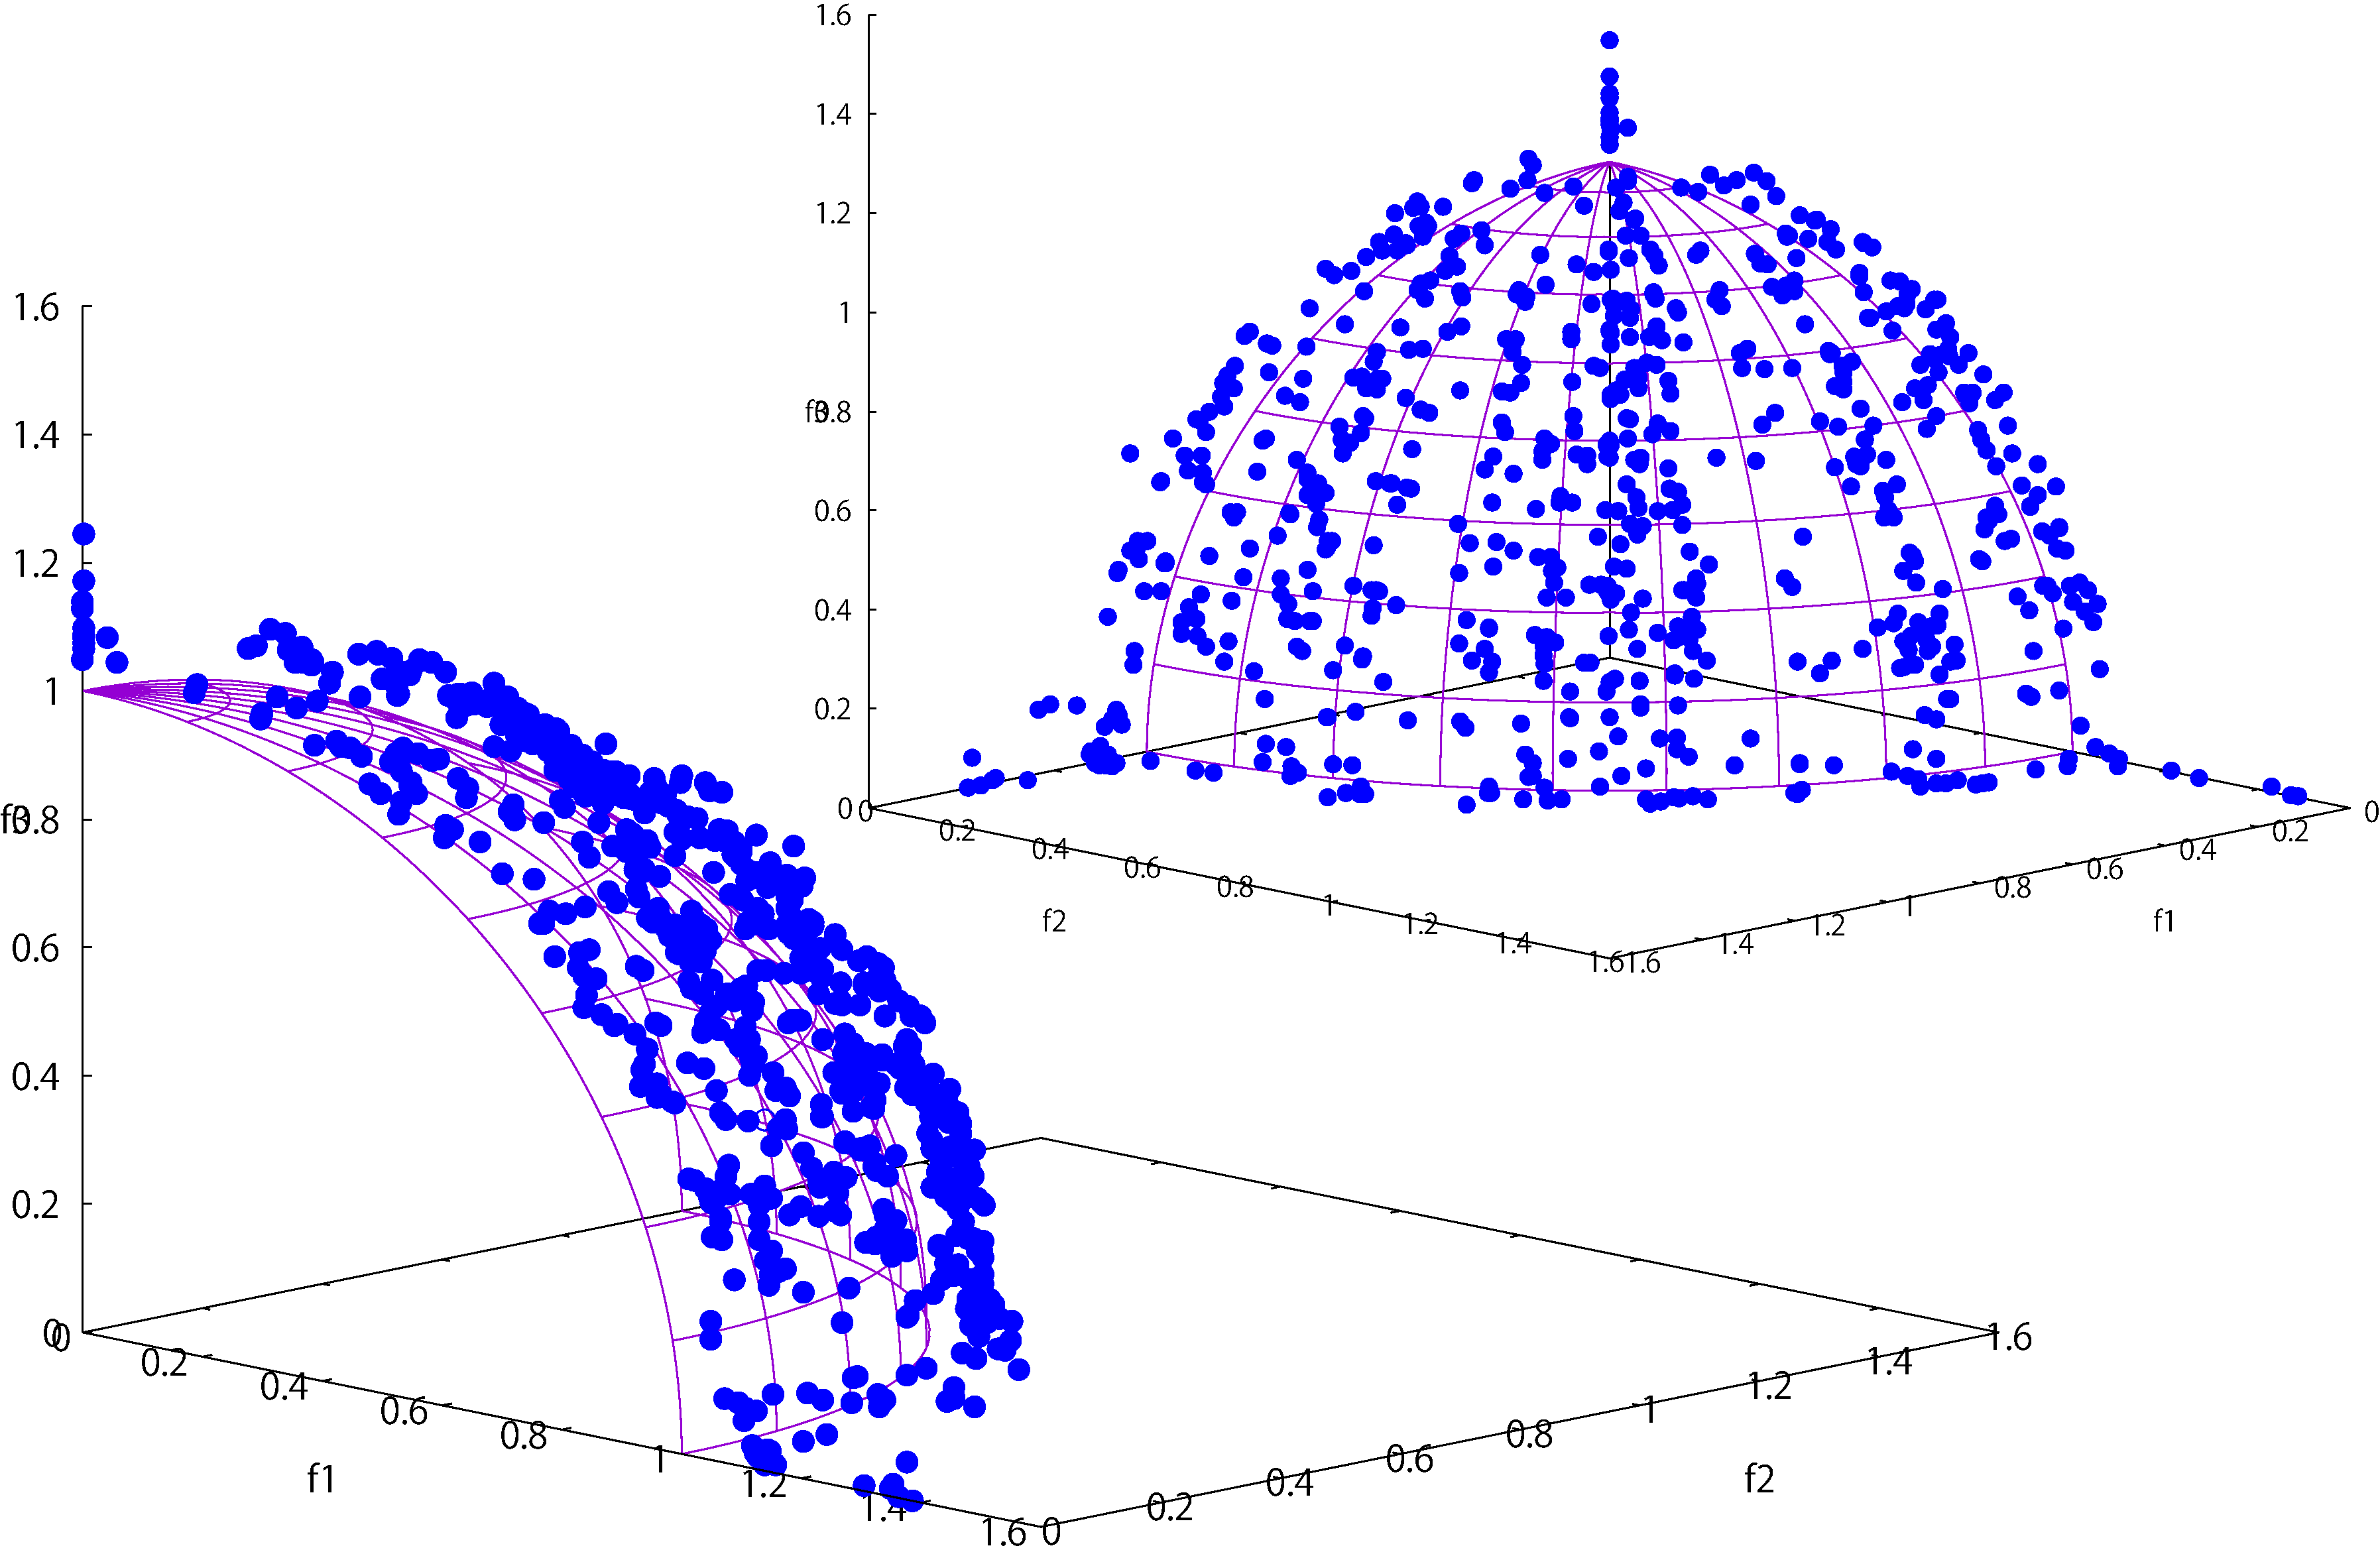
\includegraphics[width=1\linewidth]{../figures/NSGA-II/modDTLZ2_digi16_double.pdf}
\centering
{\footnotesize (b) 16桁}
\caption{Modified DTLZ2における非劣解の分布(NSGA-II)}
\label{fig:dist_mod2_nsgaii}
\end{minipage}
\begin{minipage}{0.32\hsize}
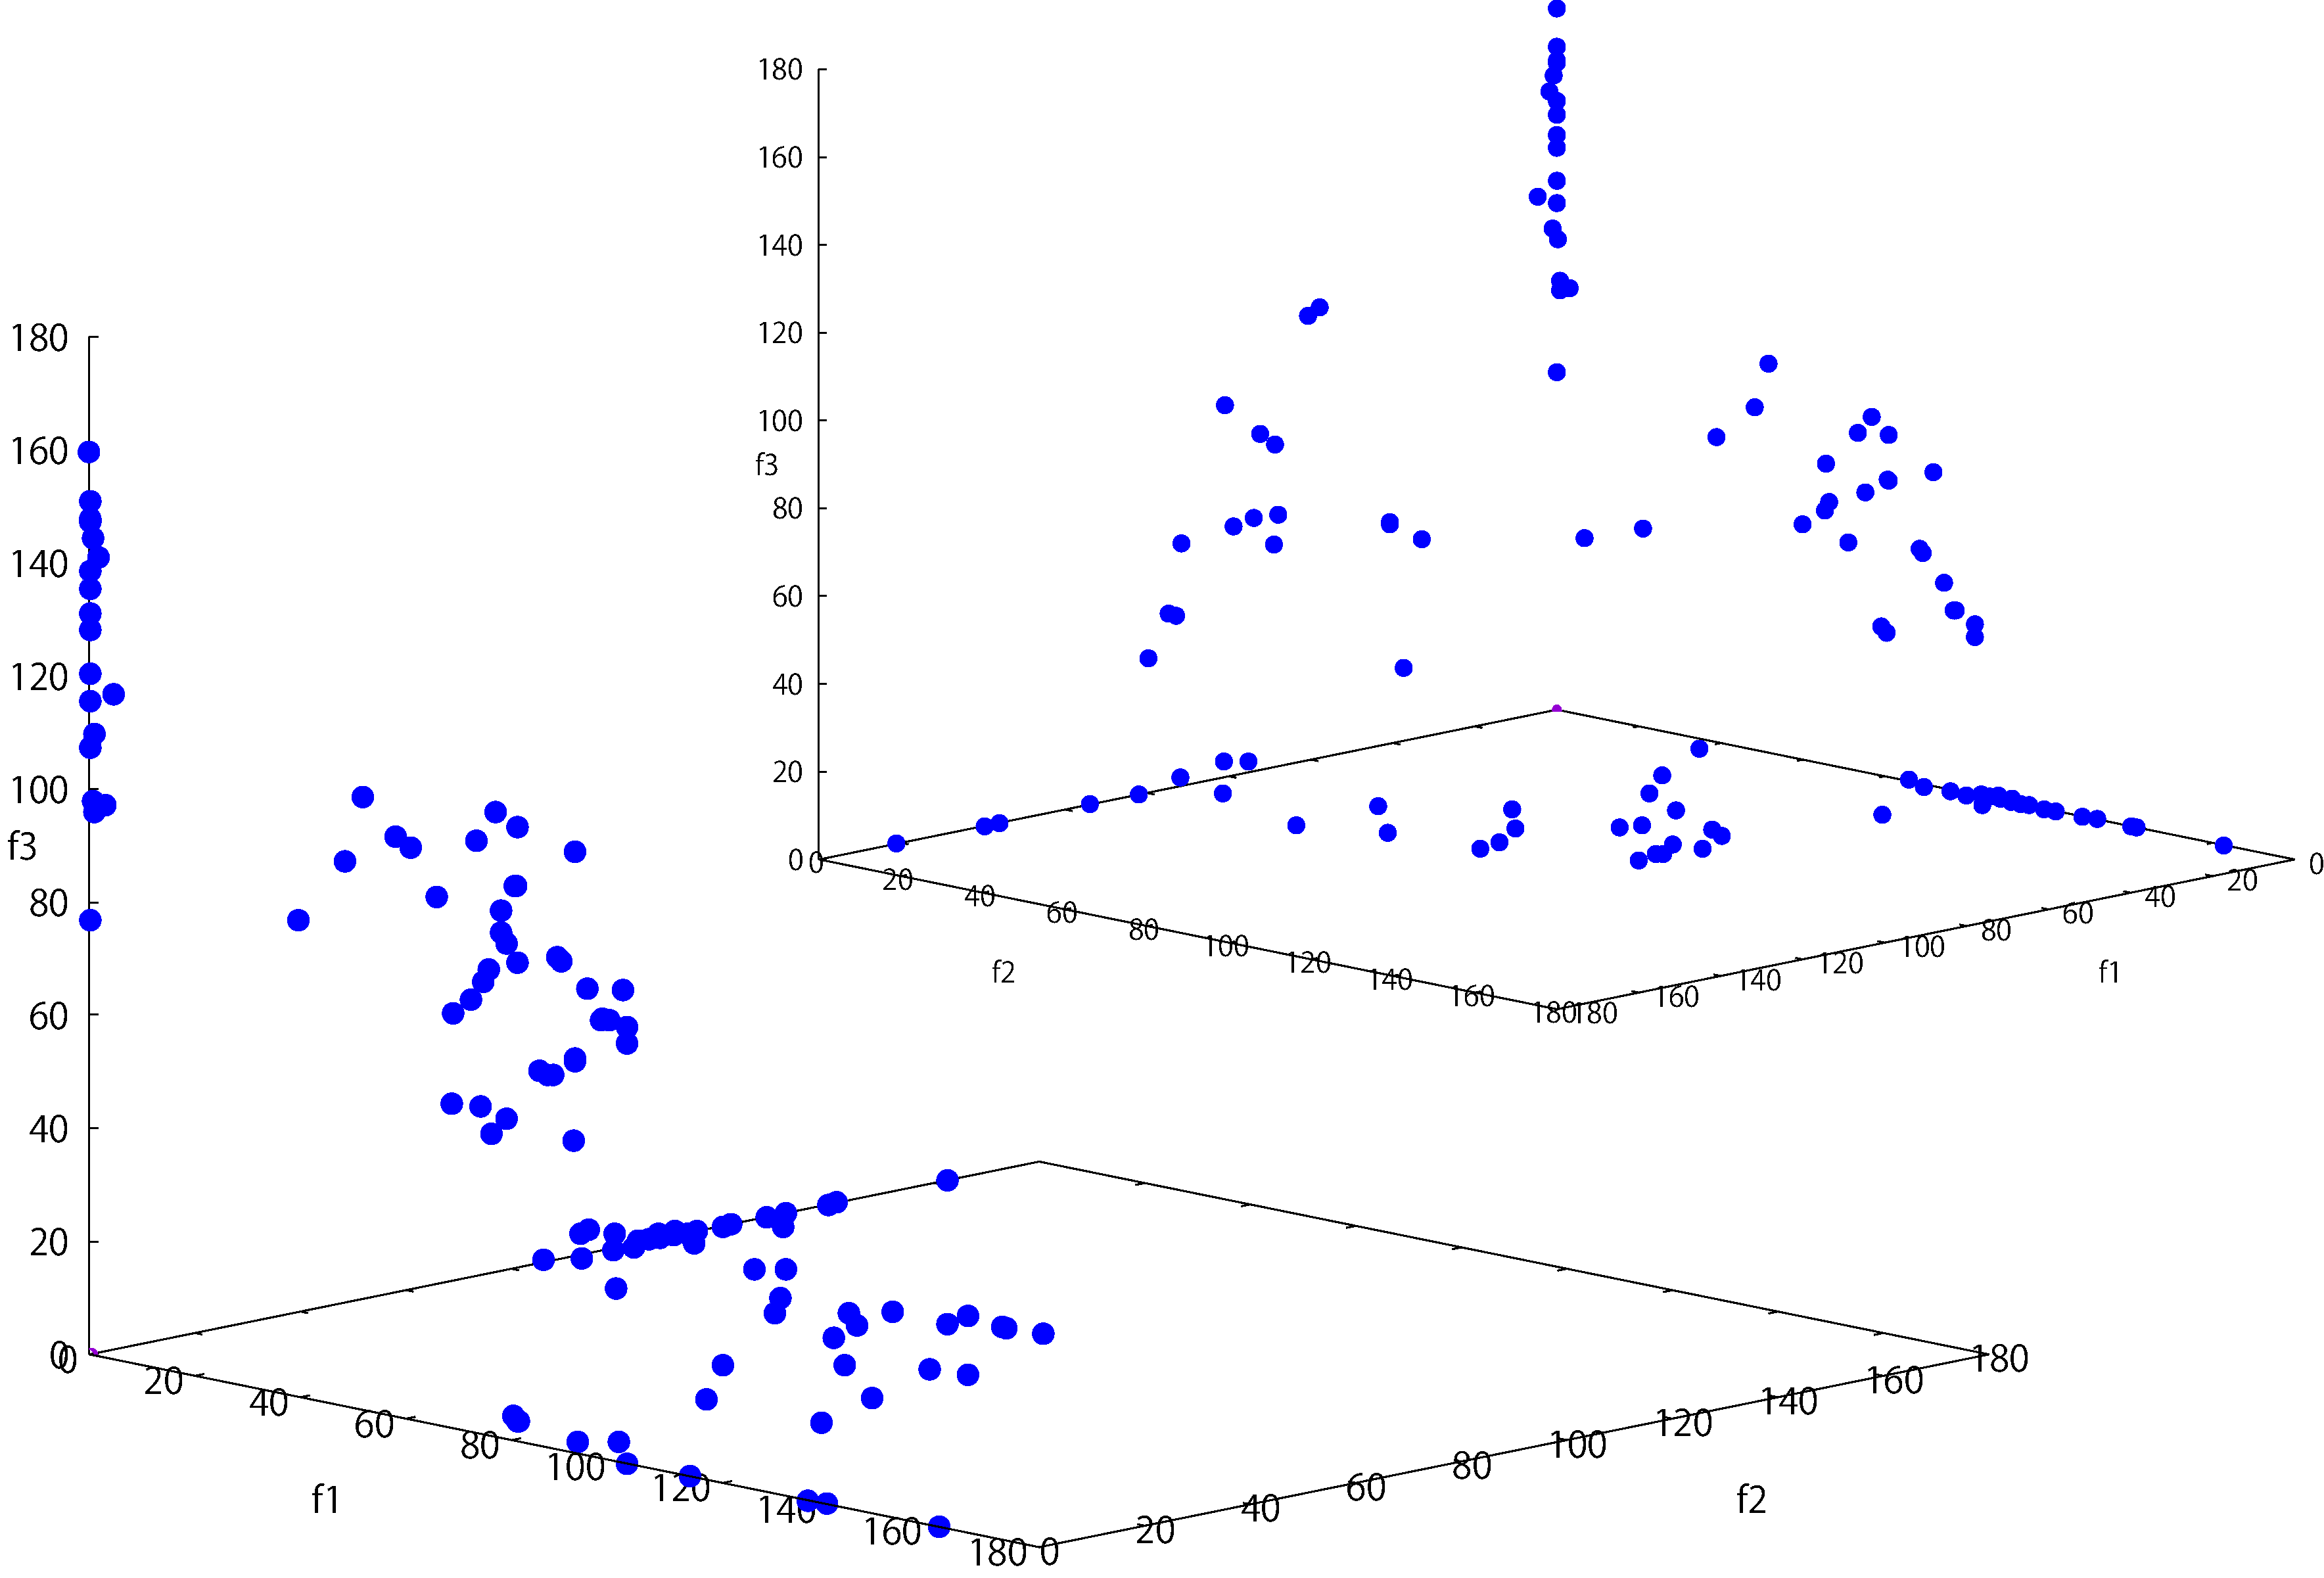
\includegraphics[width=1\linewidth]{../figures/NSGA-II/modDTLZ3_digi16_double.pdf}
\centering
{\footnotesize (b) 16桁}
\caption{Modified DTLZ3における非劣解の分布(NSGA-II)}
\label{fig:dist_mod3_nsgaii}
\end{minipage}
\begin{minipage}{0.32\hsize}
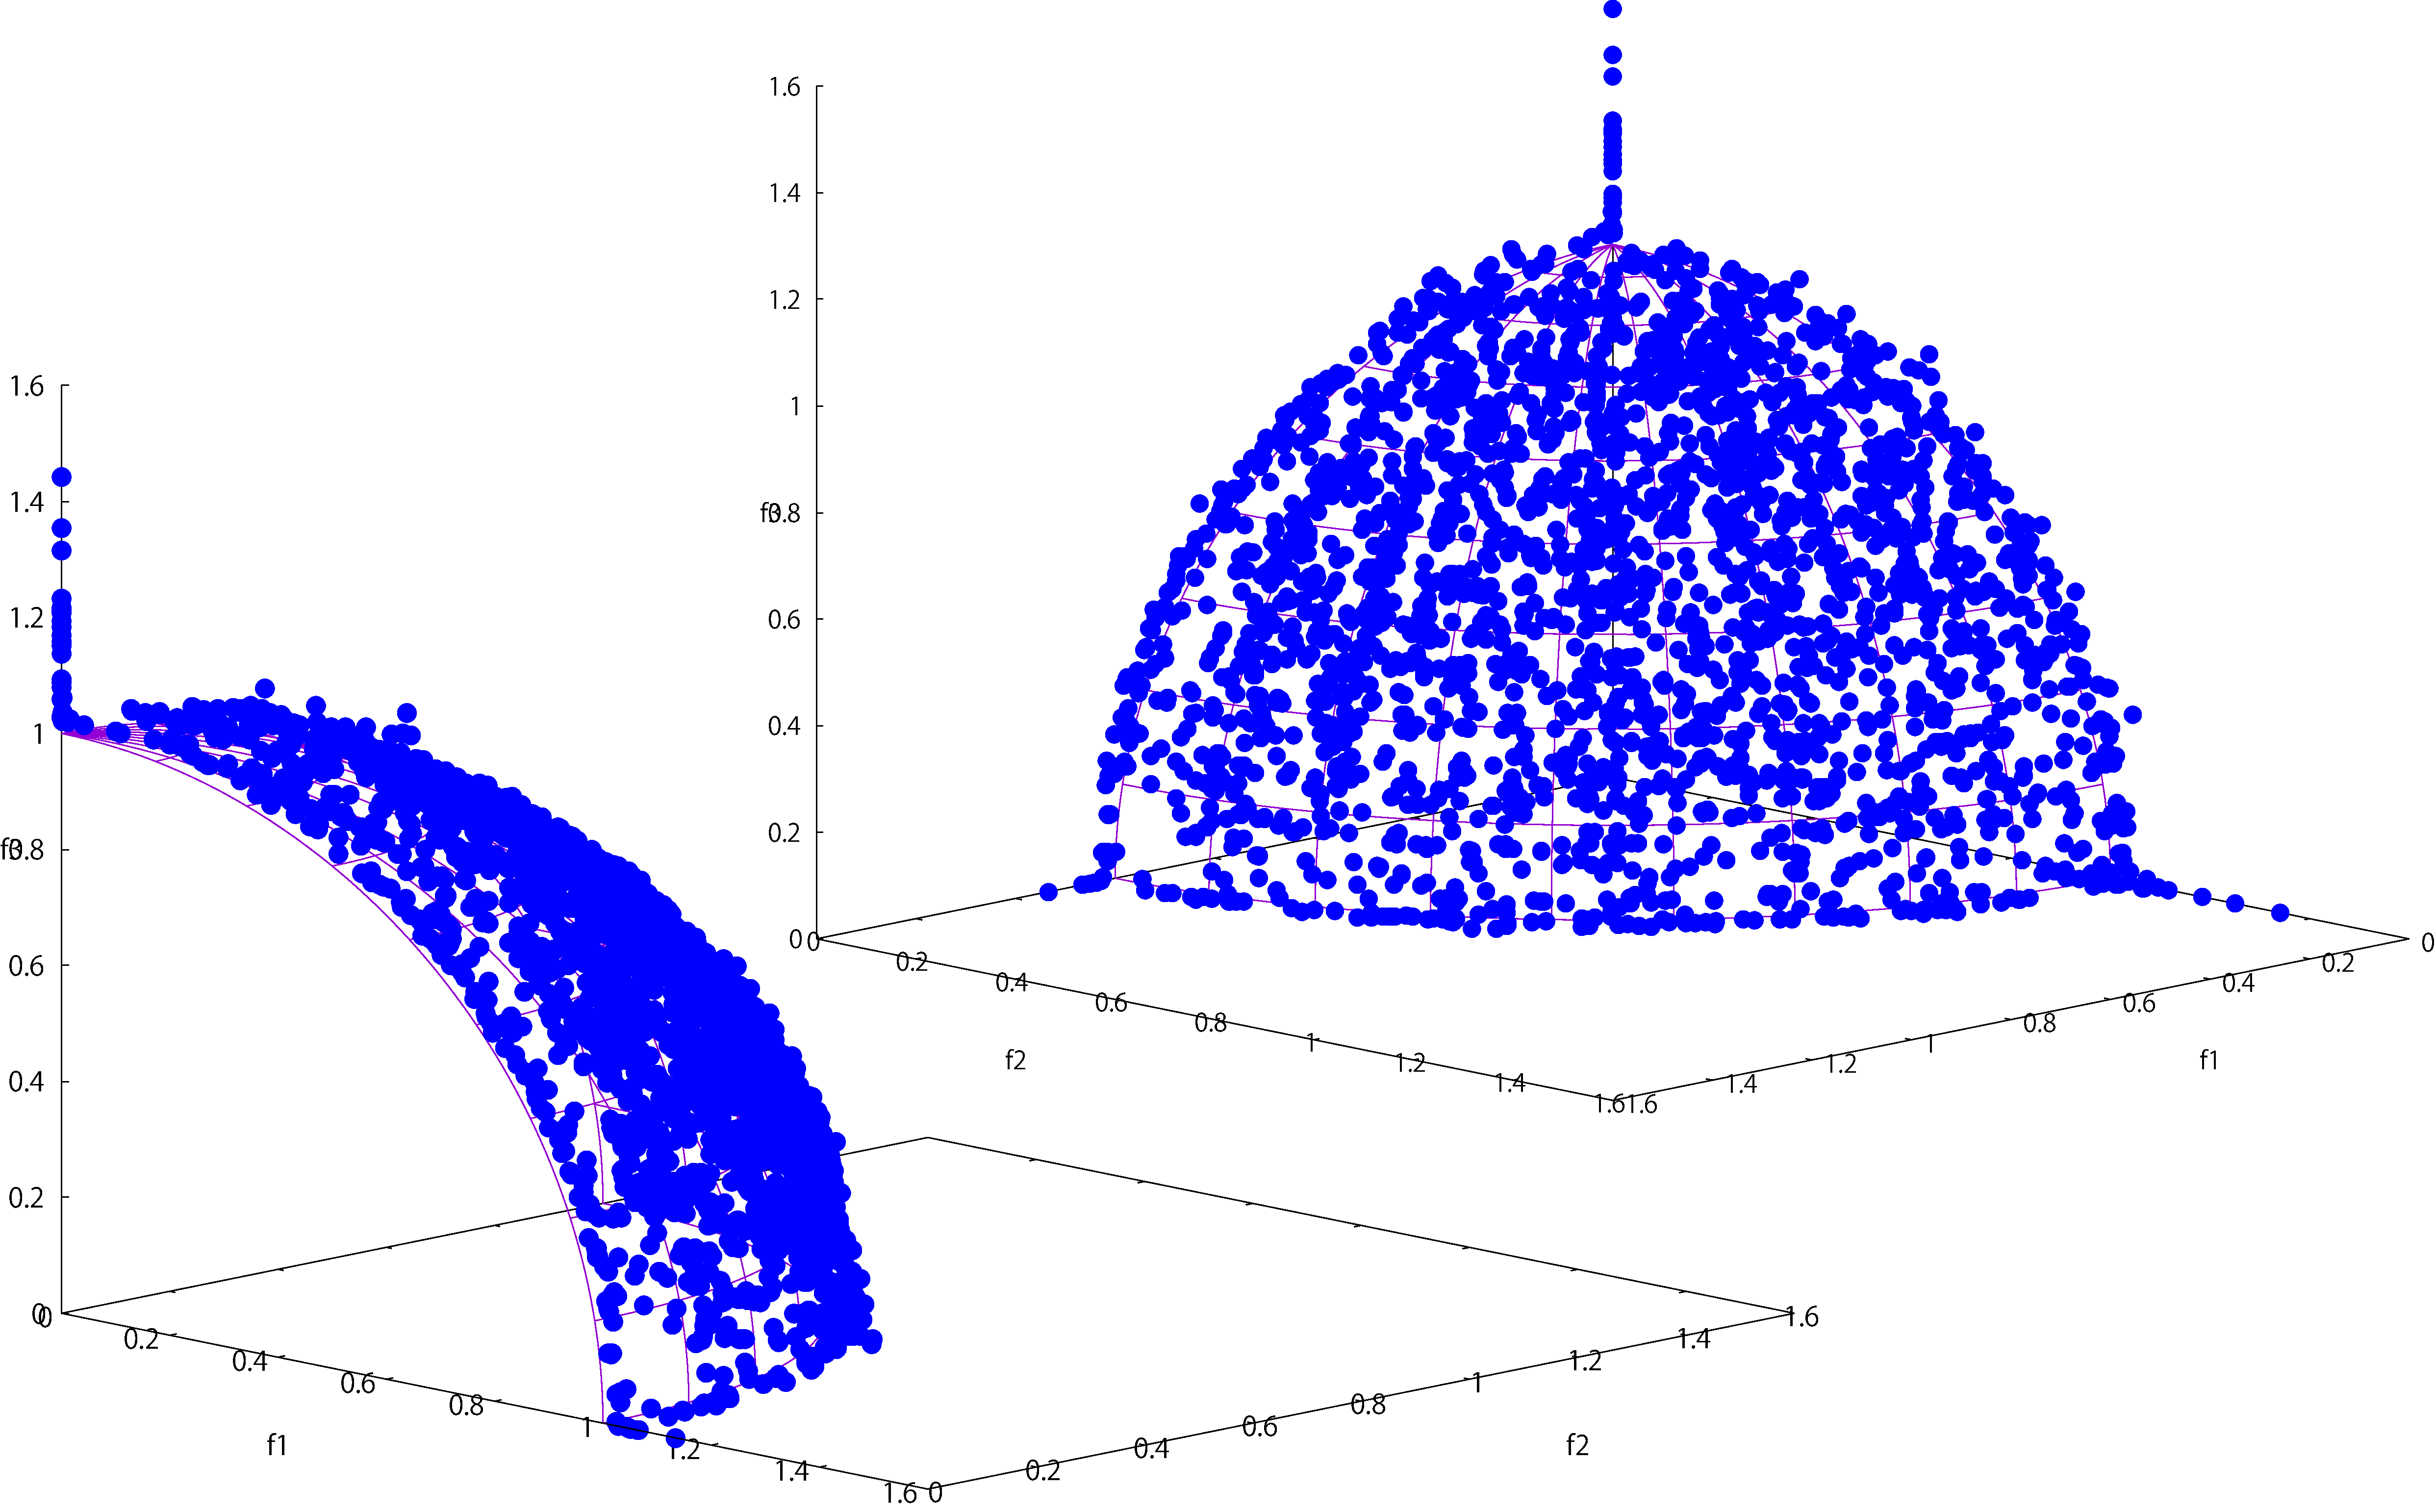
\includegraphics[width=1\linewidth]{../figures/NSGA-II/ano_DTLZ4_digi16_double.pdf}
\centering
{\footnotesize (b) 16桁}
\caption{Modified DTLZ4における非劣解の分布(NSGA-II)}
\label{fig:dist_mod4_nsgaii}
\end{minipage}
\end{tabular}
\end{figure*}

\clearpage

\subsection{MOEA/D}
\Tabref{tbl:gd_moead}はMOEA/Dにおいて,各ベンチマーク問題における各制御(小数点以下2,4,6,8,16桁)で得られたGDの平均値の推移を示している.
多目的最適化では,最終世代の結果だけではなく収束速度も重要であるため,GDの平均値は10世代目,最終世代の半分,最終世代での結果を示している.
表中に示す Obj. は目的関数の数,Var. は設計変数の数,Gen は GD の平均値を求めた世代数を示している.
また,各世代において最小値となっている値は太字で示した.

\Tabref{tbl:gd_moead}より,最終的なGDの値を見ると大半の問題は小さい桁数のものの方が小さい値となっている.
またDTLZ問題,WFG4,CDTLZ問題,Welded Beam Design 問題,Modified DTLZ2,4においては最終的な値だけでなく進化の序盤からGD値が低く,収束速度が向上していることが分かる.
しかしながら,Modified DTLZ3では2桁が最も悪い結果となっている.
これはModified DTLZ3の最適値が無理数であるために,設計変数の粒度が粗過ぎると最適値に近い値を取ることができないためである.
WFG6やWFG7でも2桁が最も悪い結果となっており,同様の原因が考えられる.

以上の結果から,MOEA/Dにおいても,粗い離散化を施すことで解の収束性が向上する傾向があるものの,問題によっては粗く離散化しすぎると最適値に到達することができず反って収束性が悪化してしまう可能性もあることが分かった.

統計的な有意差があるか確認するため,有意水準5\%でWilcoxon の順位和検定を用いて2桁の結果と16桁の結果の比較を行った.
その結果,DTLZ2-4,UF9,WFG2,WFG7,CF2,C1DTLZ3,C3DTLZ1,Welded Beam Design 問題,Modified DTLZ2-4で統計的な有意差が確認された.


%DTLZ2,DTLZ3,UF,CDTLZでは桁数が小さいほど(粗く離散化するほど)IGDは小さくなっていることが分かる.
%IGDは値が小さいほど解の収束性・多様性が良いことを表す指標であることから,桁数が小さいほど(粗く離散化するほど)これらのベンチマーク問題では解の多様性も向上していることが分かる.
%しかしながら,DTLZ4やModified DTLZ4では桁数が小さいほど悪い結果となっており,桁数が大きいものの方が良い結果となっている.
%これは先行研究でも触れたように,DTLZ4の式の構造上,目的関数の位置を司る変数(位置変数)に高い精度がなければ解が多様に広がらないからである.
%したがって,問題によって多様性を維持するためには必要最低限の桁数が存在することが分かった.

\begin{table*}[htbp]
\fontsize{7.5pt}{7.5pt} \selectfont
\tabcolsep = 1.5pt
\centering
\caption{制御桁数の違いによるGDの平均値の推移(MOEA/D)}
\label{tbl:gd_moead}
\begin{tabular}{c|ccccc|c|c|c|c|c}
\hline 
problem & MG & PS & Obj. & Var. & Gen & 2-digit & 4-digit & 6-digit & 8-digit & 16-digit \\ 
\cline{7-11}
&&&&&&GD&GD&GD&GD&GD\\
\hline
\multirow{3}{*}{DTLZ2} &        &  & &     & 10 &$\bf{1.195}$ & $1.358$ & $1.326$ & $1.400$ & $1.388$\\
  				   & 100 & 91 & 3 & 38 & 50 &$\bf{6.997 \times 10^{-2}}$ & $9.901 \times 10^{-2}$ & $1.098 \times 10^{-1}$ & $1.054 \times 10^{-1}$ & $1.066 \times 10^{-1}$\\
				   &        &     &           &   &100 & $\bf{2.508 \times 10^{-2}}$ & $3.104 \times 10^{-2}$ & $3.767 \times 10^{-2}$ & $3.482 \times 10^{-2}$ & $3.482 \times 10^{-2}$\\
\hline
\multirow{3}{*}{DTLZ3} &     &&   &       & 10 &$2.125 \times 10^{3}$ & $2.118 \times 10^{3}$ & $2.148 \times 10^{3}$ & $\bf{2.119 \times 10^{3}}$ & $2.143 \times 10^{3}$\\
  				   & 200 & 91 & 3 & 38 &100 &$\bf{1.664 \times 10^{2}}$ & $2.233 \times 10^{2}$ & $2.428 \times 10^{2}$ & $2.246 \times 10^{2}$ & $2.381 \times 10^{2}$\\
				   &        &   &&     &200 & $\bf{1.012 \times 10^{2}}$ & $1.356 \times 10^{2}$ & $1.555 \times 10^{2}$ & $1.432 \times 10^{2}$ & $1.455 \times 10^{2}$\\

\hline
\multirow{3}{*}{DTLZ4} &        &     &&  & 10 &$\bf{6.984 \times 10^{-1}}$ & $7.310 \times 10^{-1}$ & $7.218 \times 10^{-1}$ & $7.110 \times 10^{-1}$ & $7.064 \times 10^{-1}$\\
  				   & 100 & 91 & 3&38& 50 &$\bf{1.502 \times 10^{-2}}$ & $2.781 \times 10^{-2}$ & $2.893 \times 10^{-2}$ & $3.404 \times 10^{-2}$ & $2.924 \times 10^{-2}$\\
				   &        &     &&   &100 &$\bf{6.960 \times 10^{-4}}$ & $4.349 \times 10^{-3}$ & $4.382 \times 10^{-3}$ & $5.825 \times 10^{-3}$ & $4.262 \times 10^{-3}$\\
\hline
\multirow{3}{*}{UF2} &        &    &&   & 10 &$2.280 \times 10^{-1}$ & $2.295 \times 10^{-1}$ & $2.224 \times 10^{-1}$ & $\bf{2.210 \times 10^{-1}}$ & $2.215 \times 10^{-1}$\\
  				   & 100 & 100 & 2 & 20 & 50 &$3.138 \times 10^{-2}$ & $2.767 \times 10^{-2}$ & $3.275 \times 10^{-2}$ & $\bf{2.363 \times 10^{-2}}$ & $3.230 \times 10^{-2}$\\
				   &        &      &&  &100 & $1.341 \times 10^{-2}$ & $1.197 \times 10^{-2}$ & $\bf{1.099 \times 10^{-2}}$ & $1.246 \times 10^{-2}$ & $1.212 \times 10^{-2}$\\
\hline
\multirow{3}{*}{UF9} &        &    &&        & 10 &$1.687$ & $1.891$ & $\bf{1.618}$ & $1.654$ & $1.624$\\
  				   &100 & 91 & 3 & 20 & 50 &$\bf{1.789 \times 10^{-1}}$ & $2.369 \times 10^{-1}$ & $2.549 \times 10^{-1}$ & $1.926 \times 10^{-1}$ & $2.607 \times 10^{-1}$\\
				   &        &     &&   &100 &$1.360 \times 10^{-1}$ & $\bf{1.066 \times 10^{-1}}$ & $1.280 \times 10^{-1}$ & $1.368 \times 10^{-1}$ & $1.454 \times 10^{-1}$\\
\hline
\multirow{3}{*}{WFG2} &        &   &&  10  & 10 &$2.393 \times 10^{-1}$ & $\bf{2.292 \times 10^{-1}}$ & $2.457 \times 10^{-1}$ & $2.454 \times 10^{-1}$ & $2.351 \times 10^{-1}$\\
  				   & 100 & 91 & 3 & ($k=6$) &50 &$7.035 \times 10^{-2}$ & $5.726 \times 10^{-2}$ & $\bf{5.670 \times 10^{-2}}$ & $6.061 \times 10^{-2}$ & $5.483 \times 10^{-2}$\\
				   &        &      && ($l=4$) &100 &$4.472 \times 10^{-2}$ & $3.792 \times 10^{-2}$ & $3.892 \times 10^{-2}$ & $4.092 \times 10^{-2}$ & $\bf{3.763 \times 10^{-2}}$\\
\hline
\multirow{3}{*}{WFG4} &        &   &&  10  & 10 &$\bf{2.164 \times 10^{-1}}$ & $2.583 \times 10^{-1}$ & $2.551 \times 10^{-1}$ & $2.513 \times 10^{-1}$ & $2.562 \times 10^{-1}$\\
  				   & 100 & 91 & 3 & ($k=6$) & 50 &$\bf{8.391 \times 10^{-2}}$ & $9.509 \times 10^{-2}$ & $8.883 \times 10^{-2}$ & $9.053 \times 10^{-2}$ & $9.048 \times 10^{-2}$\\
				   &        &     && ($l=4$)  &100 &$\bf{6.251 \times 10^{-2}}$ & $6.751 \times 10^{-2}$ & $6.272 \times 10^{-2}$ & $6.598 \times 10^{-2}$ & $6.549 \times 10^{-2}$\\
\hline
\multirow{3}{*}{WFG6} &        &  &&  10   & 10 &$\bf{3.334 \times 10^{-1}}$ & $3.534 \times 10^{-1}$ & $3.756 \times 10^{-1}$ & $3.799 \times 10^{-1}$ & $3.782 \times 10^{-1}$\\
  				   & 100 & 91 & 3 & ($k=6$) & 50  &$1.345 \times 10^{-1}$ & $1.217 \times 10^{-1}$ & $\bf{1.060 \times 10^{-1}}$ & $1.119 \times 10^{-1}$ & $1.300 \times 10^{-1}$\\
				   &        &      && ($l=4$) &100  &$1.103 \times 10^{-1}$ & $9.912 \times 10^{-2}$ & $\bf{8.314 \times 10^{-2}}$ & $8.683 \times 10^{-2}$ & $1.012 \times 10^{-1}$\\
\hline
\multirow{3}{*}{WFG7} &        &   &&  10  & 10 &$4.227 \times 10^{-1}$ & $4.312 \times 10^{-1}$ & $4.151 \times 10^{-1}$ & $4.140 \times 10^{-1}$ & $\bf{4.119 \times 10^{-1}}$\\
  				   & 100 & 91 & 3 & ($k=6$) &50 &$1.362 \times 10^{-1}$ & $1.265 \times 10^{-1}$ & $\bf{1.065 \times 10^{-1}}$ & $1.215 \times 10^{-1}$ & $1.126 \times 10^{-1}$\\
				   &        &       && ($l=4$) &100 &$9.753 \times 10^{-2}$ & $7.751 \times 10^{-2}$ & $\bf{6.994 \times 10^{-2}}$ & $7.648 \times 10^{-2}$ & $7.060 \times 10^{-2}$\\
%\hline
\hline
\multirow{3}{*}{CF2}&        &     &&  & 10 &$\bf{5.488 \times 10^{-1}}$ & $6.057 \times 10^{-1}$ & $5.972 \times 10^{-1}$ & $5.807 \times 10^{-1}$ & $6.217 \times 10^{-1}$\\
  				   & 100 & 100 &2 & 20 & 50 &$1.176 \times 10^{-1}$ & $1.064 \times 10^{-1}$ & $1.830 \times 10^{-1}$ & $1.447 \times 10^{-1}$ & $\bf{7.748 \times 10^{-2}}$\\
				   &        &     &&   &100 &$9.811 \times 10^{-2}$ & $7.392 \times 10^{-2}$ & $1.020 \times 10^{-1}$ & $6.613 \times 10^{-2}$ & $\bf{5.864 \times 10^{-2}}$\\
\hline
\multirow{3}{*}{CF7} &        &    &&   & 10 &$2.156 \times 10$ & $2.029 \times 10$ & $\bf{1.901 \times 10}$ & $2.256 \times 10$ & $2.089 \times 10$\\
  				   & 100 & 100 &2 & 20 &50 &$2.749$ & $2.486$ & $2.679$ & $2.527$ & $\bf{2.044}$\\
				   &        &     &&   &100 &$1.931 \times 10^{-1}$ & $\bf{1.563 \times 10^{-1}}$ & $3.271 \times 10^{-1}$ & $3.148 \times 10^{-1}$ & $2.431 \times 10^{-1}$\\

\hline
\multirow{3}{*}{C1DTLZ3} &       && &       & 10 &$2.125 \times 10^{3}$ & $2.118 \times 10^{3}$ & $2.148 \times 10^{3}$ & $\bf{2.119 \times 10^{3}}$ & $2.143 \times 10^{3}$\\
                                          &200 & 91 &3 & 38 & 100 &$\bf{1.664 \times 10^{2}}$ & $2.233 \times 10^{2}$ & $2.428 \times 10^{2}$ & $2.246 \times 10^{2}$ & $2.381 \times 10^{2}$\\
				   &        &       && &200 &$\bf{1.012 \times 10^{2}}$ & $1.356 \times 10^{2}$ & $1.555 \times 10^{2}$ & $1.432 \times 10^{2}$ & $1.455 \times 10^{2}$\\
\hline
\multirow{3}{*}{C2DTLZ2} &  &&      &       & 10 &$6.438 \times 10$ & $6.440 \times 10$ & $6.451 \times 10$ & $\bf{5.44 \times 10}$ & $6.129 \times 10$\\
  				   & 100 & 91 & 3 & 38&50 &$4.790$ & $3.220$ & $1.547$ & $\bf{7.477 \times 10^{-1}}$ & $3.333$\\
		convex		   &        &     &&   &100 &$\bf{2.421 \times 10^{-1}}$ & $5.173 \times 10^{-1}$ & $3.017 \times 10^{-1}$ & $3.386 \times 10^{-1}$ & $3.588 \times 10^{-1}$\\

\hline
\multirow{3}{*}{C3DTLZ1} &       && &       & 10 &$2.259 \times 10^{3}$ & $2.339 \times 10^{3}$ & $\bf{2.208 \times 10^{3}}$ & $\bf{2.208 \times 10^{3}}$ & $2.249 \times 10^{3}$\\
                                          &200 & 91 & 3 & 38 &100 &$\bf{2.096 \times 10^{2}}$ & $6.017 \times 10^{2}$ & $5.565 \times 10^{2}$ & $7.031 \times 10^{2}$ & $6.540 \times 10^{2}$\\
				   &        &    &&    &200 &$\bf{1.935 \times 10^{2}}$ & $7.152 \times 10^{2}$ & $5.571 \times 10^{2}$ & $7.213 \times 10^{2}$ & $6.870 \times 10^{2}$\\
				   \hline
\multirow{3}{*}{\scriptsize Car Side Impact}&  &&      &       & 10 &$\bf{1.671 \times 10^{-1}}$ & $1.764 \times 10^{-1}$ & $1.965 \times 10^{-1}$ & $1.859 \times 10^{-1}$ & $1.729 \times 10^{-1}$\\
  				   & 100 & 91 & 3 & 7 &50 &$\bf{1.000 \times 10^{-1}}$ & $1.010 \times 10^{-1}$ & $1.117 \times 10^{-1}$ & $1.160 \times 10^{-1}$ & $1.001 \times 10^{-1}$\\
				   &        &      &&  &100 &$8.003 \times 10^{-2}$ & $8.074 \times 10^{-2}$ & $8.465 \times 10^{-2}$ & $8.838 \times 10^{-2}$ & $\bf{7.410 \times 10^{-2}}$\\
\hline
\multirow{3}{*}{\fontsize{6pt}{0pt}\selectfont Welded Beam Design} & &&       &       & 10 &$\bf{3.694}$ & $4.989$ & $4.504$ & $4.694$ & $4.714$\\
  				   & 100 & 100 & 2 & 4 &50 &$\bf{1.434}$ & $2.848$ & $2.403$ & $2.673$ & $2.542$\\
				   &        &      &&  &100 &$\bf{4.077 \times 10^{-1}}$ & $2.173$ & $1.806$ & $1.574$ & $1.342$\\
\hline
\multirow{3}{*}{\fontsize{6.5pt}{0pt}\selectfont Modified DTLZ2} & &&       &       & 10 &$\bf{1.101}$ & $1.242$ & $1.182$ & $1.255$ & $1.276$\\
  				   & 100 & 91 & 3 & 38 &50 &$\bf{5.043 \times 10^{-2}}$ & $7.508 \times 10^{-2}$ & $8.641 \times 10^{-2}$ & $9.118 \times 10^{-2}$ & $8.34 \times 10^{-2}$\\
				   &        &      &&  &100 &$\bf{8.224 \times 10^{-3}}$ & $1.248 \times 10^{-2}$ & $1.577 \times 10^{-2}$ & $1.580 \times 10^{-2}$ & $1.558 \times 10^{-2}$\\
\hline
\multirow{3}{*}{\fontsize{6.5pt}{0pt}\selectfont Modified DTLZ3} & &&       &       & 10 &$2.261 \times 10^{3}$ & $\bf{2.224 \times 10^{3}}$ & $2.242 \times 10^{3}$ & $2.263 \times 10^{3}$ & $2.236 \times 10^{3}$\\
  				   & 200 & 91 & 3 & 38 &100 &$3.035 \times 10^{2}$ & $2.434 \times 10^{2}$ & $\bf{2.209 \times 10^{2}}$ & $2.392 \times 10^{2}$ & $2.729 \times 10^{2}$\\
				   &        &      &&  &200 &$2.160 \times 10^{2}$ & $1.425 \times 10^{2}$ & $\bf{1.330 \times 10^{2}}$ & $1.553 \times 10^{2}$ & $1.791 \times 10^{2}$\\
\hline
\multirow{3}{*}{\fontsize{6.5pt}{0pt}\selectfont Modified DTLZ4} & &&       &       & 10 &$8.134 \times 10^{-1}$ & $8.361 \times 10^{-1}$ & $8.233 \times 10^{-1}$ & $\bf{8.091 \times 10^{-1}}$ & $8.312 \times 10^{-1}$\\
  				   & 100 & 91 & 3 & 38 &50 &$\bf{1.514 \times 10^{-2}}$ & $2.503 \times 10^{-2}$ & $3.847 \times 10^{-2}$ & $3.459 \times 10^{-2}$ & $3.297 \times 10^{-2}$\\
				   &        &      &&  &100 &$\bf{8.782 \times 10^{-4}}$ & $4.253 \times 10^{-3}$ & $6.094 \times 10^{-3}$ & $5.846 \times 10^{-3}$ & $6.012 \times 10^{-3}$\\

\hline

\hline\end{tabular}
\\
{\footnotesize MG = the number of generation set; PS = the number of population size set.}\\
{\footnotesize Obj. = the number of objectives; Var. = the number of variables.}\\
{\footnotesize Gen = the generation that results were computed on.} \\
{\footnotesize $k$ = position parameter in WFG problems; $l$ = distance parameter in WFG problems.}\\
\end{table*}

\begin{table*}[htbp]
\fontsize{7.5pt}{7.5pt} \selectfont
\tabcolsep = 1.5pt
%\tabcolsep = 1.5pt
\centering
\caption{制御桁数の違いによるIGDの平均値の推移(MOEA/D)}
\label{tbl:igd_moead}
\begin{tabular}{c|ccccc|c|c|c|c|c}
\hline 
problem & MG & PS & Obj. & Var. & Gen & 2-digit & 4-digit & 6-digit & 8-digit & 16-digit \\ 
%\cmidrule(r){3-9}
%\hline 
\cline{7-11}
&&&&&&IGD&IGD&IGD&IGD&IGD\\
%\cline{3-5}
\hline
\multirow{3}{*}{DTLZ2} &  &&      &       & 10 &$\bf{9.228 \times 10^{-1}}$ & $9.313 \times 10^{-1}$ & $9.680 \times 10^{-1}$ & $9.856 \times 10^{-1}$ & $9.716 \times 10^{-1}$\\
  				  &100 & 91 & 3 & 38 & 50 & $\bf{1.181 \times 10^{-1}}$ & $1.368 \times 10^{-1}$ & $1.347 \times 10^{-1}$ & $1.322 \times 10^{-1}$ & $1.435 \times 10^{-1}$\\
				   &        &   &&     &100 &$7.419 \times 10^{-2}$ & $7.524 \times 10^{-2}$ & $\bf{7.300 \times 10^{-2}}$ & $7.600 \times 10^{-2}$ & $7.470 \times 10^{-2}$\\
\hline
\multirow{3}{*}{DTLZ3} &      &&  &       & 10 &$1.591 \times 10^{3}$ & $\bf{1.437 \times 10^{3}}$ & $1.533 \times 10^{3}$ & $1.487 \times 10^{3}$ & $1.540 \times 10^{3}$\\
  				   &200 & 91 & 3 & 38 & 100 &$\bf{1.586 \times 10^{2}}$ & $2.021 \times 10^{2}$ & $2.156 \times 10^{2}$ & $1.992 \times 10^{2}$ & $2.070 \times 10^{2}$\\
				   &        &      &&  &200 &$\bf{9.52 \times 10}$ & $1.283 \times 10^{2}$ & $1.448 \times 10^{2}$ & $1.335 \times 10^{2}$ & $1.363 \times 10^{2}$\\

\hline
\multirow{3}{*}{DTLZ4} &   &&     &       & 10 &$1.047$ & $\bf{1.027}$ & $1.157$ & $1.152$ & $1.153$\\
  				   &100 & 91  & 3 & 38 & 50 &$\bf{5.469 \times 10^{-1}}$ & $5.673 \times 10^{-1}$ & $6.926 \times 10^{-1}$ & $5.818 \times 10^{-1}$ & $6.685 \times 10^{-1}$\\
				   &        &     &&   &100 &$\bf{5.03 \times 10^{-1}}$ & $5.145 \times 10^{-1}$ & $6.759 \times 10^{-1}$ & $5.499 \times 10^{-1}$ & $6.174 \times 10^{-1}$\\
\hline
\multirow{3}{*}{UF2} &        &     &&       & 10 &$\bf{2.079 \times 10^{-1}}$ & $2.231 \times 10^{-1}$ & $2.182 \times 10^{-1}$ & $2.163 \times 10^{-1}$ & $2.159 \times 10^{-1}$\\
  				   &100 & 100 & 2 & 20 & 50 &$1.449 \times 10^{-1}$ & $1.401 \times 10^{-1}$ & $\bf{1.235 \times 10^{-1}}$ & $1.282 \times 10^{-1}$ & $1.252 \times 10^{-1}$\\
				   &        &    &&    &100 &$1.228 \times 10^{-1}$ & $1.386 \times 10^{-1}$ & $\bf{1.121 \times 10^{-1}}$ & $1.209 \times 10^{-1}$ & $1.153 \times 10^{-1}$\\

\hline
\multirow{3}{*}{UF9} &        &    &&        & 10 &$8.739 \times 10^{-1}$ & $1.023$ & $9.048 \times 10^{-1}$ & $8.810 \times 10^{-1}$ & $\bf{8.336 \times 10^{-1}}$\\
  				   &100 & 91 & 3 & 20 & 50 &$5.032 \times 10^{-1}$ & $\bf{4.604 \times 10^{-1}}$ & $4.815 \times 10^{-1}$ & $4.887 \times 10^{-1}$ & $4.675 \times 10^{-1}$\\
				   &        &     &&   &100 &$4.703 \times 10^{-1}$ & $\bf{4.010 \times 10^{-1}}$ & $4.101 \times 10^{-1}$ & $4.422 \times 10^{-1}$ & $4.109 \times 10^{-1}$\\
\hline
\multirow{3}{*}{WFG2} &      &&  &   10    & 10 &$5.545 \times 10^{-1}$ & $\bf{5.455 \times 10^{-1}}$ & $5.716 \times 10^{-1}$ & $5.771 \times 10^{-1}$ & $5.751 \times 10^{-1}$\\
  				   &100 & 91 & 3 & ($k = 6$) & 50 &$4.03 \times 10^{-1}$ & $\bf{3.701 \times 10^{-1}}$ & $3.818 \times 10^{-1}$ & $3.760 \times 10^{-1}$ & $3.938 \times 10^{-1}$\\
				   &        &   &&  ($l=4$)   &100 &$4.028 \times 10^{-1}$ & $3.395 \times 10^{-1}$ & $3.529 \times 10^{-1}$ & $\bf{3.473 \times 10^{-1}}$ & $3.631 \times 10^{-1}$\\
\hline
\multirow{3}{*}{WFG4} &      &&  &   10    & 10 &$\bf{3.700 \times 10^{-1}}$ & $4.31 \times 10^{-1}$ & $4.34 \times 10^{-1}$ & $4.245 \times 10^{-1}$ & $4.174 \times 10^{-1}$\\
  				   &100 & 91 & 3 & ($k=6$) & 50 &$2.313 \times 10^{-1}$ & $2.313 \times 10^{-1}$ & $\bf{2.248 \times 10^{-1}}$ & $2.292 \times 10^{-1}$ & $2.301 \times 10^{-1}$\\
				   &        &&&  ($l=4$)      &100 &$2.274 \times 10^{-1}$ & $2.276 \times 10^{-1}$ & $\bf{2.203 \times 10^{-1}}$ & $2.260 \times 10^{-1}$ & $2.298 \times 10^{-1}$\\
\hline
\multirow{3}{*}{WFG6} &       && &   10    & 10 & $\bf{6.306 \times 10^{-1}}$ & $6.710 \times 10^{-1}$ & $6.806 \times 10^{-1}$ & $6.931 \times 10^{-1}$ & $6.755 \times 10 ^{-1}$\\
  				   &100 & 91 & 3 & ($k=6$) & 50  &$3.142 \times 10^{-1}$ & $2.899 \times 10^{-1}$ & $2.824 \times 10^{-1}$ & $\bf{2.813 \times 10^{-1}}$ & $2.960 \times 10^{-1}$\\
				   &        &  &&  ($l=4$)    &100  &$2.944 \times 10^{-1}$ & $2.686 \times 10^{-1}$ & $2.618 \times 10^{-1}$ & $\bf{2.553 \times 10^{-1}}$ & $2.682 \times 10^{-1}$\\
\hline
\multirow{3}{*}{WFG7} &       && &  10     & 10 &$\bf{5.156 \times 10^{-1}}$ & $5.401 \times 10^{-1}$ & $5.324 \times 10^{-1}$ & $5.329 \times 10^{-1}$ & $5.335 \times 10^{-1}$\\
  				   &100 & 91 & 3 &  ($k=6$)& 50 &$3.200 \times 10^{-1}$ & $3.180 \times 10^{-1}$ & $3.223 \times 10^{-1}$ & $3.275 \times 10^{-1}$ & $\bf{3.155 \times 10^{-1}}$\\
				   &        &    && ($l=4$)   &100 &$3.092 \times 10^{-1}$ & $3.080 \times 10^{-1}$ & $3.061 \times 10^{-1}$ & $3.083 \times 10^{-1}$ & $\bf{3.058 \times 10^{-1}}$\\				   			   
\hline
\multirow{3}{*}{CF2} &        &    &&   & 10 &$4.530 \times 10^{-1}$ & $4.786 \times 10^{-1}$ & $4.468 \times 10^{-1}$ & $\bf{4.451 \times 10^{-1}}$ & $4.526 \times 10^{-1}$\\
  				   &100 & 100 & 2 & 20 & 50 &$1.849 \times 10^{-1}$ & $1.661 \times 10^{-1}$ & $1.669 \times 10^{-1}$ & $\bf{1.618 \times 10^{-1}}$ & $1.797 \times 10^{-1}$\\
				   &   &&     &        &100 &$1.628 \times 10^{-1}$ & $1.616 \times 10^{-1}$ & $1.650 \times 10^{-1}$ & $\bf{1.573 \times 10^{-1}}$ & $1.777 \times 10^{-1}$\\
\hline
\multirow{3}{*}{CF7} &   &&     &       & 10 &$\bf{1.580 \times 10}$ & $1.725 \times 10$ & $1.584 \times 10$ & $1.639 \times 10$ & $1.635 \times 10$\\
  				   &100 & 100 & 2 & 20 & 50 &$2.111$ & $2.037$ & $2.222$ & $1.994$ & $\bf{1.733}$\\
				   &        &    &&    &100 &$5.142 \times 10^{-1}$ & $\bf{4.444 \times 10^{-1}}$ & $5.091 \times 10^{-1}$ & $5.527 \times 10^{-1}$ & $5.620 \times 10^{-1}$\\

\hline
\multirow{3}{*}{C1DTLZ3} &      &&  &     & 10 &$1.591 \times 10^{3}$ & $\bf{1.437 \times 10^{3}}$ & $1.533 \times 10^{3}$ & $1.487 \times 10^{3}$ & $1.540 \times 10^{3}$\\
                                          &200 & 91 & 3 & 38 & 100 &$\bf{1.586 \times 10^{2}}$ & $2.021 \times 10^{2}$ & $2.156 \times 10^{2}$ & $1.992 \times 10^{2}$ & $2.070 \times 10^{2}$\\
				   &        &  &&      &200 &$\bf{9.52 \times 10}$ & $1.283 \times 10^{2}$ & $1.448 \times 10^{2}$ & $1.335 \times 10^{2}$ & $1.363 \times 10^{2}$\\
\hline
\multirow{3}{*}{C2DTLZ2} &   &&     &       & 10 &$\bf{1.257}$ & $1.412$ & $1.408$ & $1.278$ & $1.382$\\
  				   &100 & 91 & 3 & 38 & 50 &$1.413 \times 10^{-1}$ & $\bf{1.359 \times 10^{-1}}$ & $1.442 \times 10^{-1}$ & $1.505 \times 10^{-1}$ & $1.461 \times 10^{-1}$\\
			convex	   &        &    &&    &100  &$1.178 \times 10^{-1}$ & $1.168 \times 10^{-1}$ & $\bf{1.146 \times 10^{-1}}$ & $1.198 \times 10^{-1}$ & $1.197 \times 10^{-1}$\\

\hline
\multirow{3}{*}{C3DTLZ1} &        &   &&    & 10 &$1.525 \times 10^{3}$ & $\bf{1.425 \times 10^{3}}$ & $1.483 \times 10^{3}$ & $1.485 \times 10^{3}$ & $1.549 \times 10^{3}$\\
                                          &200 & 91 &3 & 38 & 100 &$\bf{1.650 \times 10^{2}}$ & $2.149 \times 10^{2}$ & $2.237 \times 10^{2}$ & $2.104 \times 10^{2}$ & $2.420 \times 10^{2}$\\
				   &        &    &&    &200 &$\bf{9.670 \times 10}$ & $1.477 \times 10^{2}$ & $1.468 \times 10^{2}$ & $1.457 \times 10^{2}$ & $1.635 \times 10^{2}$\\
\hline
\multirow{3}{*}{\scriptsize Car Side Impact} &  &&      &       & 10 &$1.46$ & $1.435$ & $\bf{1.336}$ & $1.379$ & $1.46$\\
  				   &100 & 91 & 3 & 7 & 50 &$6.464 \times 10^{-1}$ & $\bf{5.599 \times 10^{-1}}$ & $6.409 \times 10^{-1}$ & $6.622 \times 10^{-1}$ & $5.899 \times 10^{-1}$\\
				   &        &   &&     &100 &$4.407 \times 10^{-1}$ & $3.492 \times 10^{-1}$ & $3.753 \times 10^{-1}$ & $3.965 \times 10^{-1}$ & $\bf{3.389 \times 10^{-1}}$\\
\hline
\multirow{3}{*}{\fontsize{6pt}{0pt}\selectfont Welded Beam Design} &   &&     &       & 10 &$\bf{1.722}$ & $2.040$ & $2.033$ & $2.051$ & $1.914$\\
  				   &100 & 100 & 2 & 4 & 50 &$\bf{1.667}$ & $2.000$ & $1.823$ & $1.976$ & $1.928$\\
				   &        &     &&   &100 &$\bf{1.613}$ & $2.012$ & $1.908$ & $2.059$ & $2.004$\\
\hline
\multirow{3}{*}{\fontsize{6.5pt}{0pt}\selectfont Modified DTLZ2} & &&       &       & 10 &$\bf{9.21 \times 10^{-1}}$ & $1.001$ & $9.780 \times 10^{-1}$ & $1.024$ & $1.024$\\
  				   & 100 & 91 & 3 & 38 &50 &$\bf{1.199 \times 10^{-1}}$ & $1.407 \times 10^{-1}$ & $1.446 \times 10^{-1}$ & $1.553 \times 10^{-1}$ & $1.387 \times 10^{-1}$\\
				   &        &      &&  &100 &$\bf{7.286 \times 10^{-2}}$ & $7.382 \times 10^{-2}$ & $7.490 \times 10^{-2}$ & $7.815 \times 10^{-2}$ & $7.627 \times 10^{-2}$\\
\hline
\multirow{3}{*}{\fontsize{6.5pt}{0pt}\selectfont Modified DTLZ3} & &&       &       & 10 &$1.645 \times 10^{3}$ & $\bf{1.598 \times 10^{3}}$ & $1.650 \times 10^{3}$ & $1.656 \times 10^{3}$ & $1.616 \times 10^{3}$\\
  				   & 200 & 91 & 3 & 38 &100 &$2.924 \times 10^{2}$ & $2.221 \times 10^{2}$ & $\bf{1.968 \times 10^{2}}$ & $2.170 \times 10^{2}$ & $2.461 \times 10^{2}$\\
				   &        &      &&  &200 &$2.082 \times 10^{2}$ & $1.322 \times 10^{2}$ & $\bf{1.255 \times 10^{2}}$ & $1.444 \times 10^{2}$ & $1.693 \times 10^{2}$\\
\hline
\multirow{3}{*}{\fontsize{6.5pt}{0pt}\selectfont Modified DTLZ4} & &&       &       & 10 &$1.126$ & $1.179$ & $1.104$ & $\bf{1.089}$ & $1.102$\\
  				   & 100 & 91 & 3 & 38 &50 &$5.909 \times 10^{-1}$ & $5.855 \times 10^{-1}$ & $\bf{5.143 \times 10^{-1}}$ & $5.214 \times 10^{-1}$ & $5.804 \times 10^{-1}$\\
				   &        &      &&  &100 &$5.541 \times 10^{-1}$ & $4.641 \times 10^{-1}$ & $4.338 \times 10^{-1}$ & $3.989 \times 10^{-1}$ & $\bf{3.949 \times 10^{-1}}$\\
			   
\hline\end{tabular}
\\
{\footnotesize MG = the number of generation set; PS = the number of population size set.}\\
{\footnotesize Obj. = the number of objectives; Var. = the number of variables.}\\
{\footnotesize Gen = the generation that results were computed on.} \\
{\footnotesize $k$ = position parameter in WFG problems; $l$ = distance parameter in WFG problems.}\\
\end{table*}
\afterpage{\clearpage}

\Tabref{tbl:igd_moead}はMOEA/Dにおいて,各ベンチマーク問題における各制御(小数点以下2,4,6,8,16桁)で得られたIGDの平均値の推移を示している.
表の見方は\Tabref{tbl:gd_moead}と同様である.
\Tabref{tbl:igd_nsgaii}より,DTLZ3,DTLZ4,C1DTLZ3,C3DTLZ1,Welded Beam Design 問題,Modified DTLZ2においては世代を通して優れたIGD値となっていることが分かる.
DTLZ4では,NSGA-IIのIGDの結果では最低だった2桁の結果が最も良い結果となった.
これは2桁では安定的に小さいIGDが得られているが,他の制御では試行ごとのばらつきが大きく平均値が上昇してしまったものと考えられる.
そのため,最良値で比較した場合は2桁が最も悪い結果となっている.
WFG問題では,どの問題でも最終的なIGD値は悪い結果となっている.
しかしながらどの問題においても進化の序盤は小さい桁数の方が小さい値となっていることから,探索能力向上の傾向が見られる.
しかし,桁数を小さくしすぎると,多様な解を得るために必要な粒度の細かさが足りず,最終的にIGDが悪化してしまったことが考えられる.

次に,特徴的な結果が見られたDTLZ2-4とModified DTLZ2-4の結果を詳しく見る.

\Figref{fig:gd_dtlz_moead}はDTLZ2-4のGDの世代ごとの推移を示している.
\Figref{fig:gd_dtlz_moead}の結果から,いずれの問題も2桁の結果が最も良い結果となっていることが分かる.
この結果から,NSGA-IIの結果同様,DTLZでは粗い離散化により収束性が向上することが確認できた.

\Figref{fig:igd_dtlz_moead}はDTLZ2-4のIGDの世代ごとの推移を示している.
\Figref{fig:igd_dtlz_moead}の結果から,DTLZ3やDTLZ4においては2桁の結果が良い結果となっていることが分かる.

\Figref{ogawaku--n},\ref{kondouku--n},\ref{katorisa--n}はそれぞれ,DTLZ2-4において2桁と16桁を用いた場合に得られた非劣解集合を示している.
\Figref{ogawaku--n}の結果から,DTLZ2においては2桁と16桁で得られる非劣解集合には大きな差はないことが分かった.
\Figref{kondouku--n}の結果から,16桁に比べ2桁の方が明らかに最適化方向である原点方向に解が生成されており,解の収束性が高いことが分かる.
\Figref{katorisa--n}では,16桁は紫で示した真のパレートフロントを覆うように解が生成されている一方で,2桁は局所的にしか非劣解が得られていない.
しかしながら,IGDの結果は良い結果となっていることから,16桁の結果は試行ごとのばらつきが大きくIGDの平均値が上昇してしまったことが考えられる.
また,このことからも,DTLZ4では設計変数を細かい粒度を用いて探索しなければ,パレートフロントを覆うような解を生成することができないことが分かった.

\Figref{fig:gd_mod_moead}はModified DTLZ2-4のGDの世代ごとの推移を示している.
\Figref{fig:gd_mod_moead}の結果から,Modified DTLZ2,4では桁数が小さいほど収束性が良いことが分かる.
一方で,Modified DTLZ3では2桁が最も悪い結果となっていることが分かる.
NSGA-IIの結果と同様に,Modified DTLZ3では最適値が無理数であることから,2桁では厳密に最適値に到達することができず,その結果収束性が悪化してしまったことが考えられる.



%\afterpage{\clearpage}
\begin{figure*}[htbp]
\begin{tabular}{cc}
\begin{minipage}{0.32\hsize}
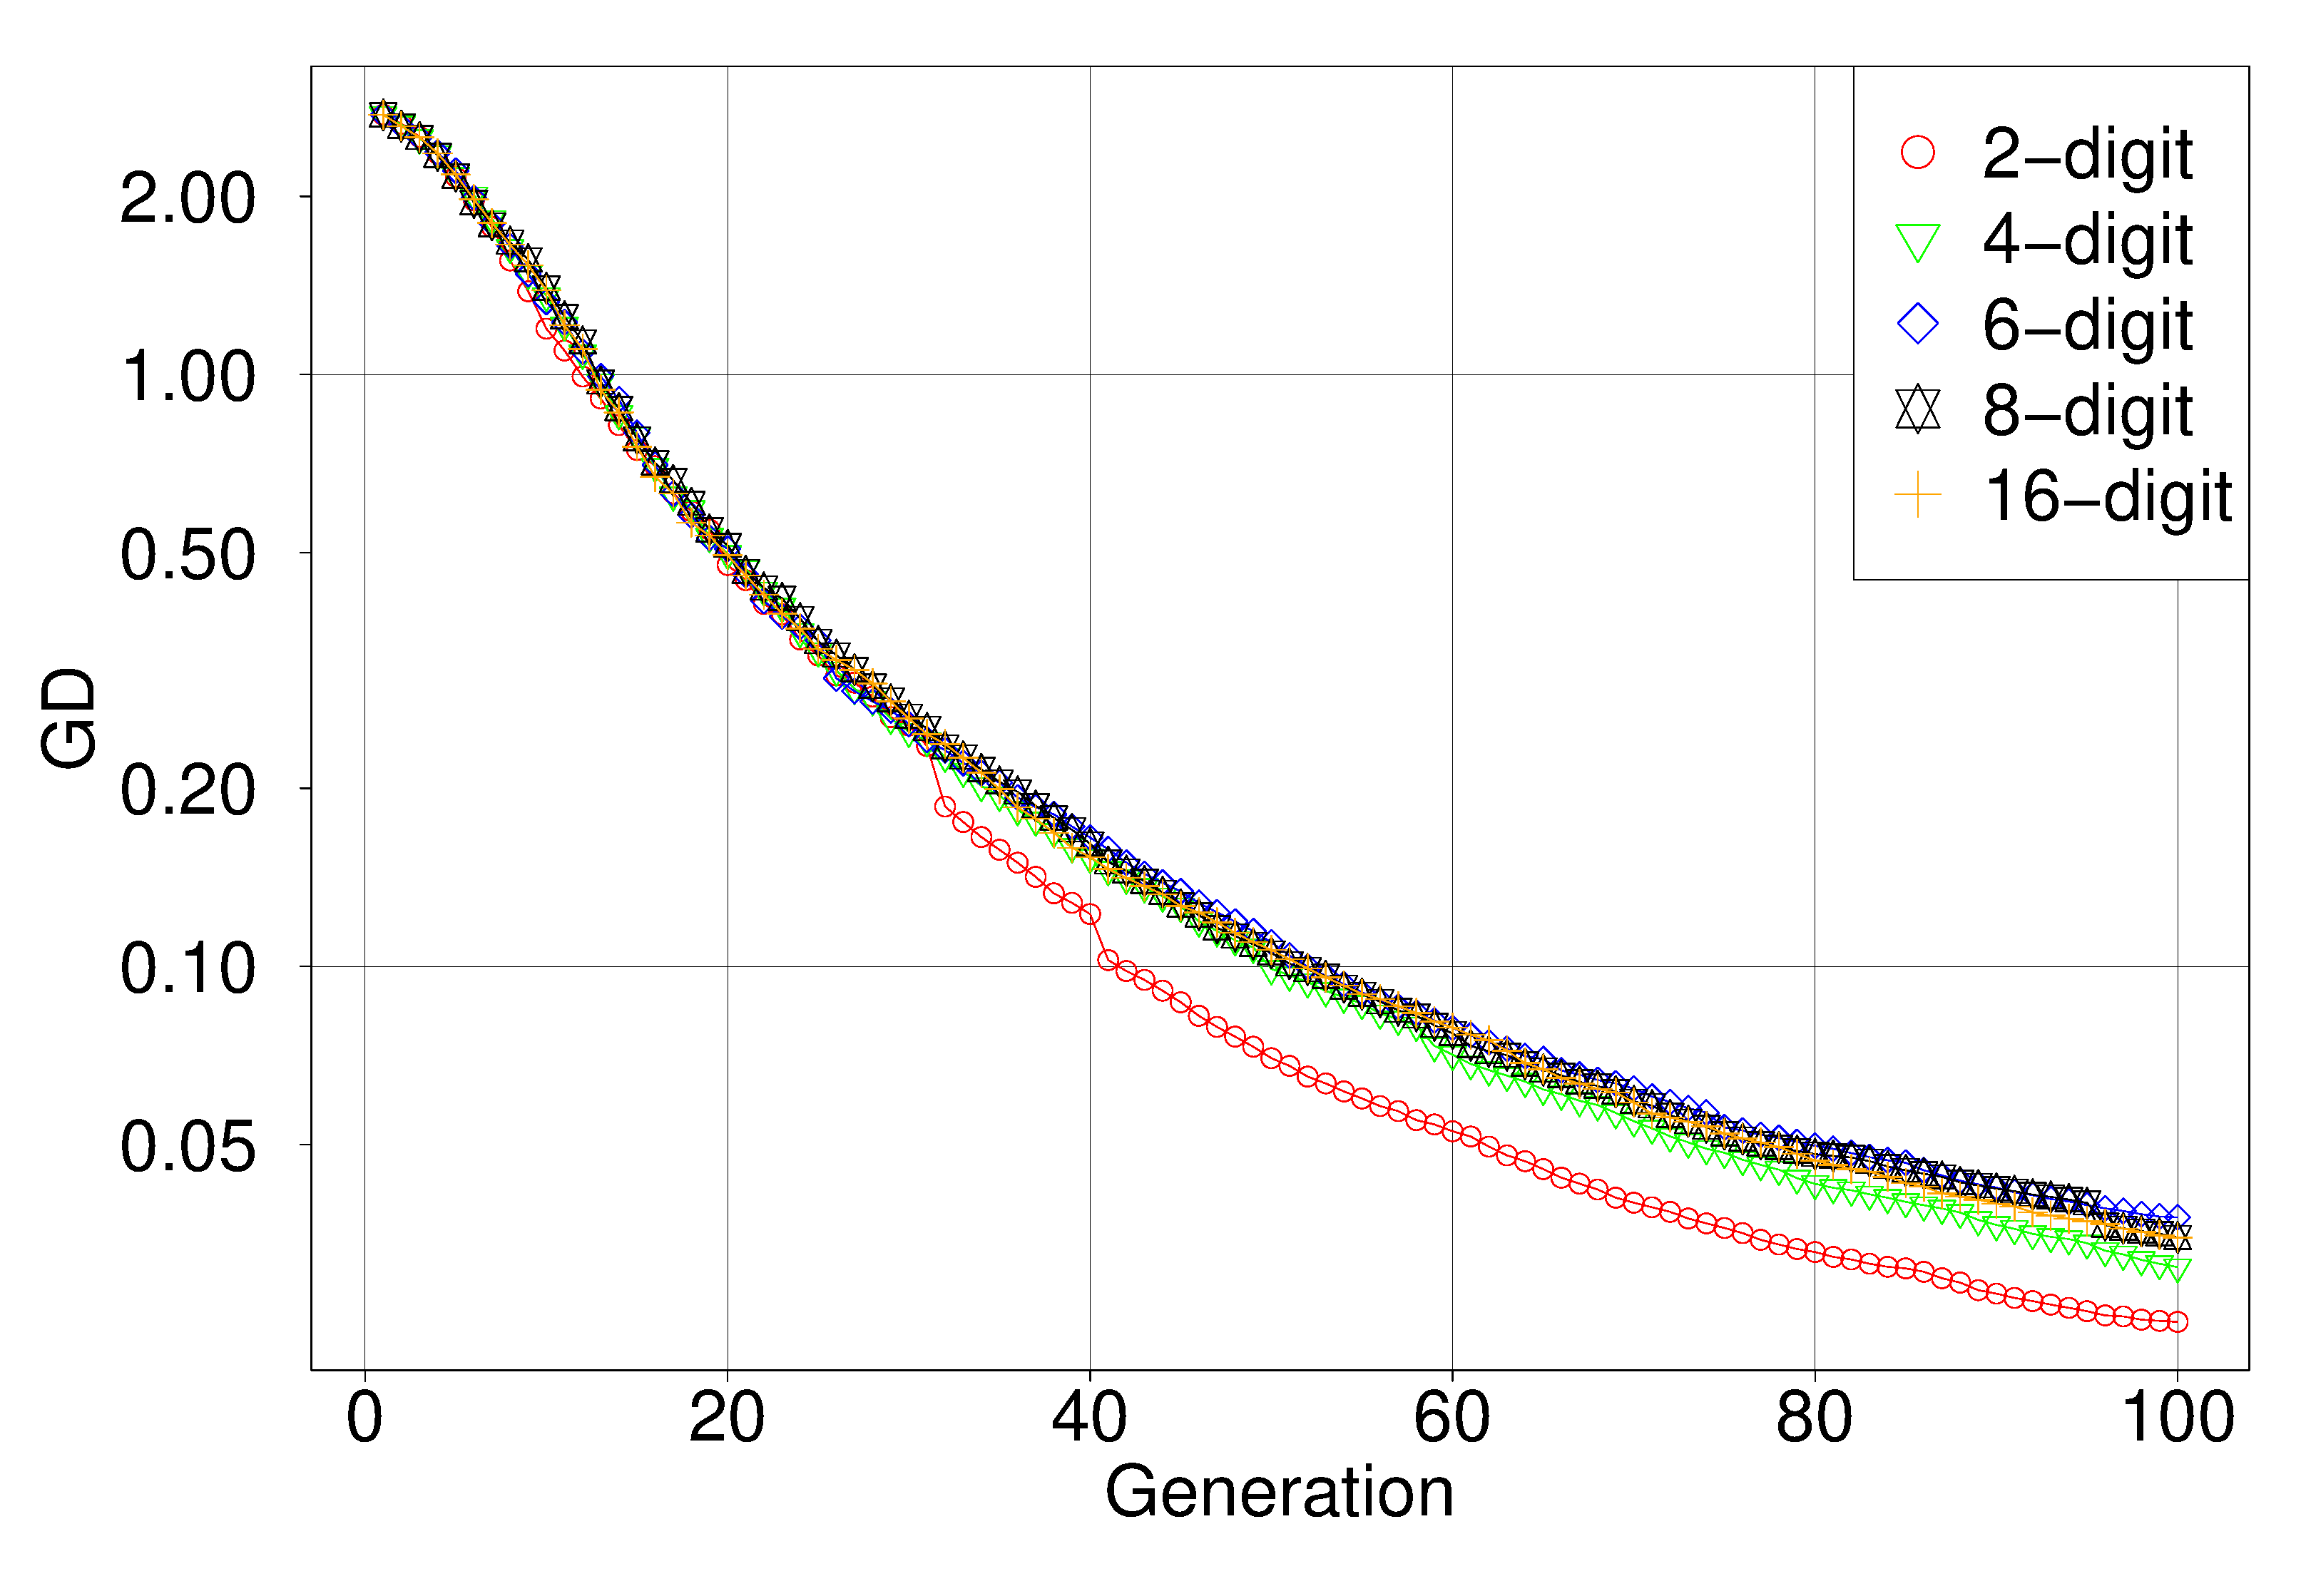
\includegraphics[width=1\linewidth]{../figures/MOEAD/DTLZ2_GD.eps}
\begin{center}
{\footnotesize (a) DTLZ2}
\end{center}
\end{minipage}
\begin{minipage}{0.32\hsize}
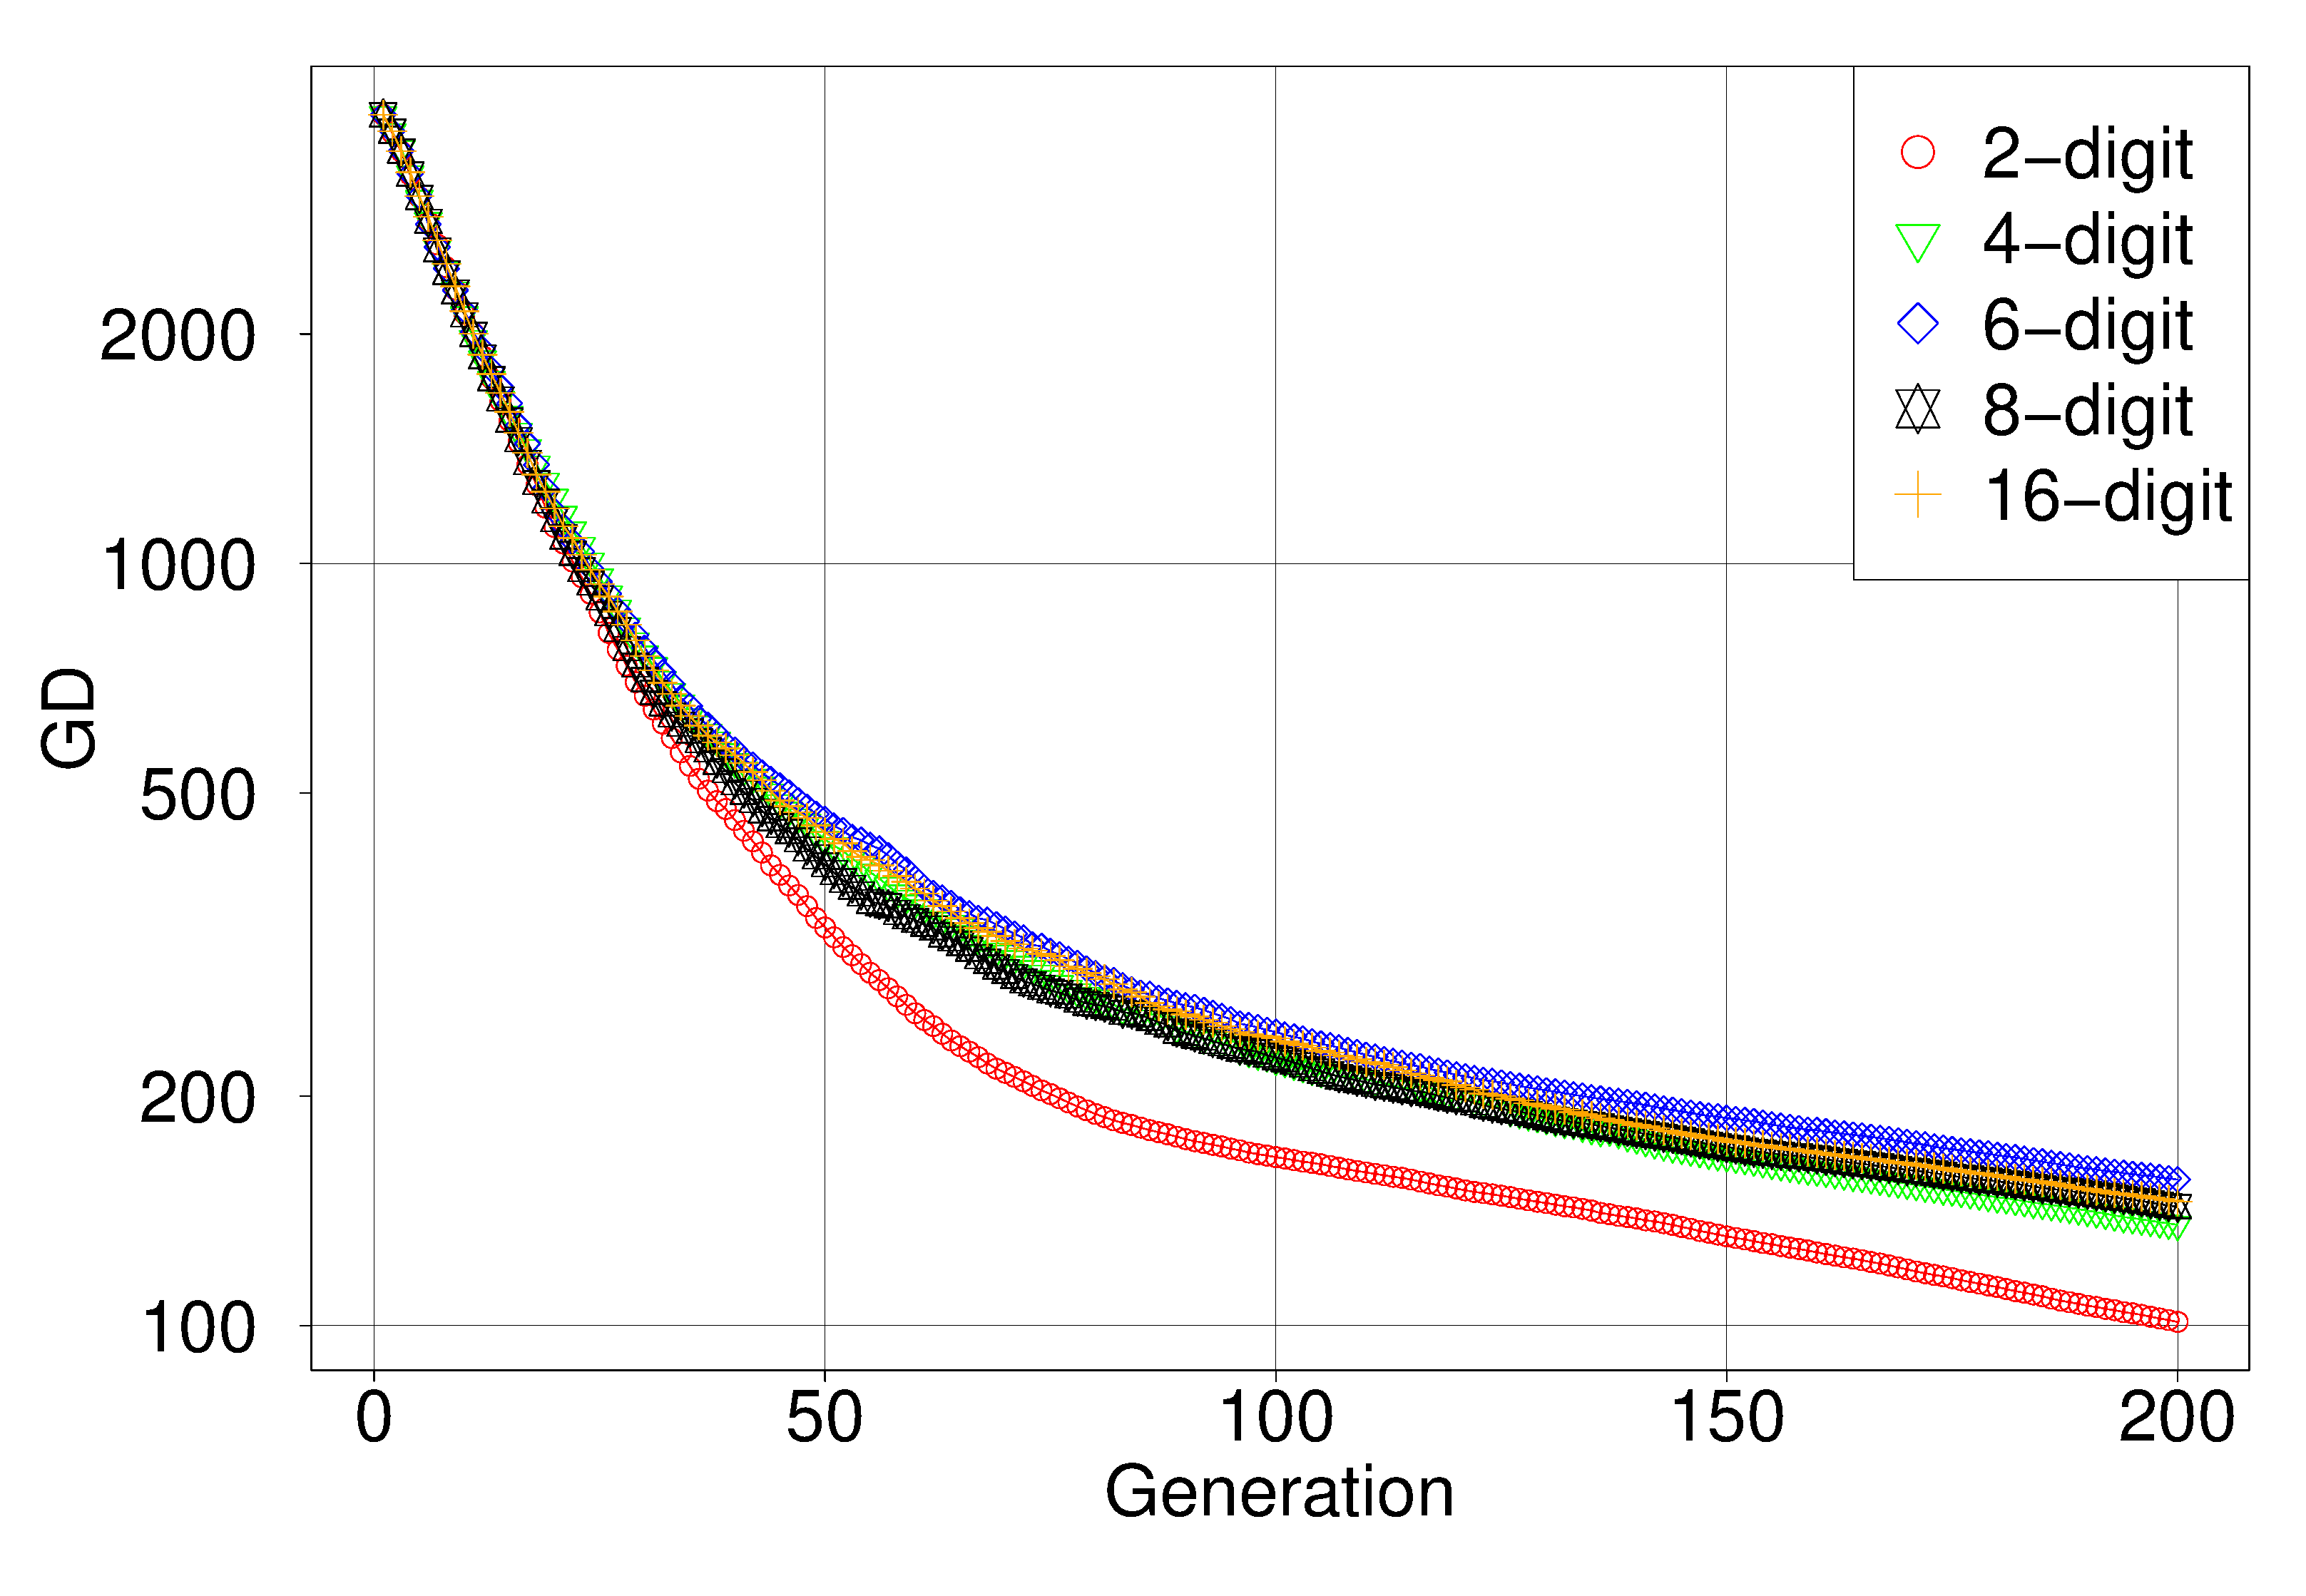
\includegraphics[width=1\linewidth]{../figures/MOEAD/DTLZ3_GD.eps}
\begin{center}
{\footnotesize (b) DTLZ3}
\end{center}
\end{minipage}
\begin{minipage}{0.32\hsize}
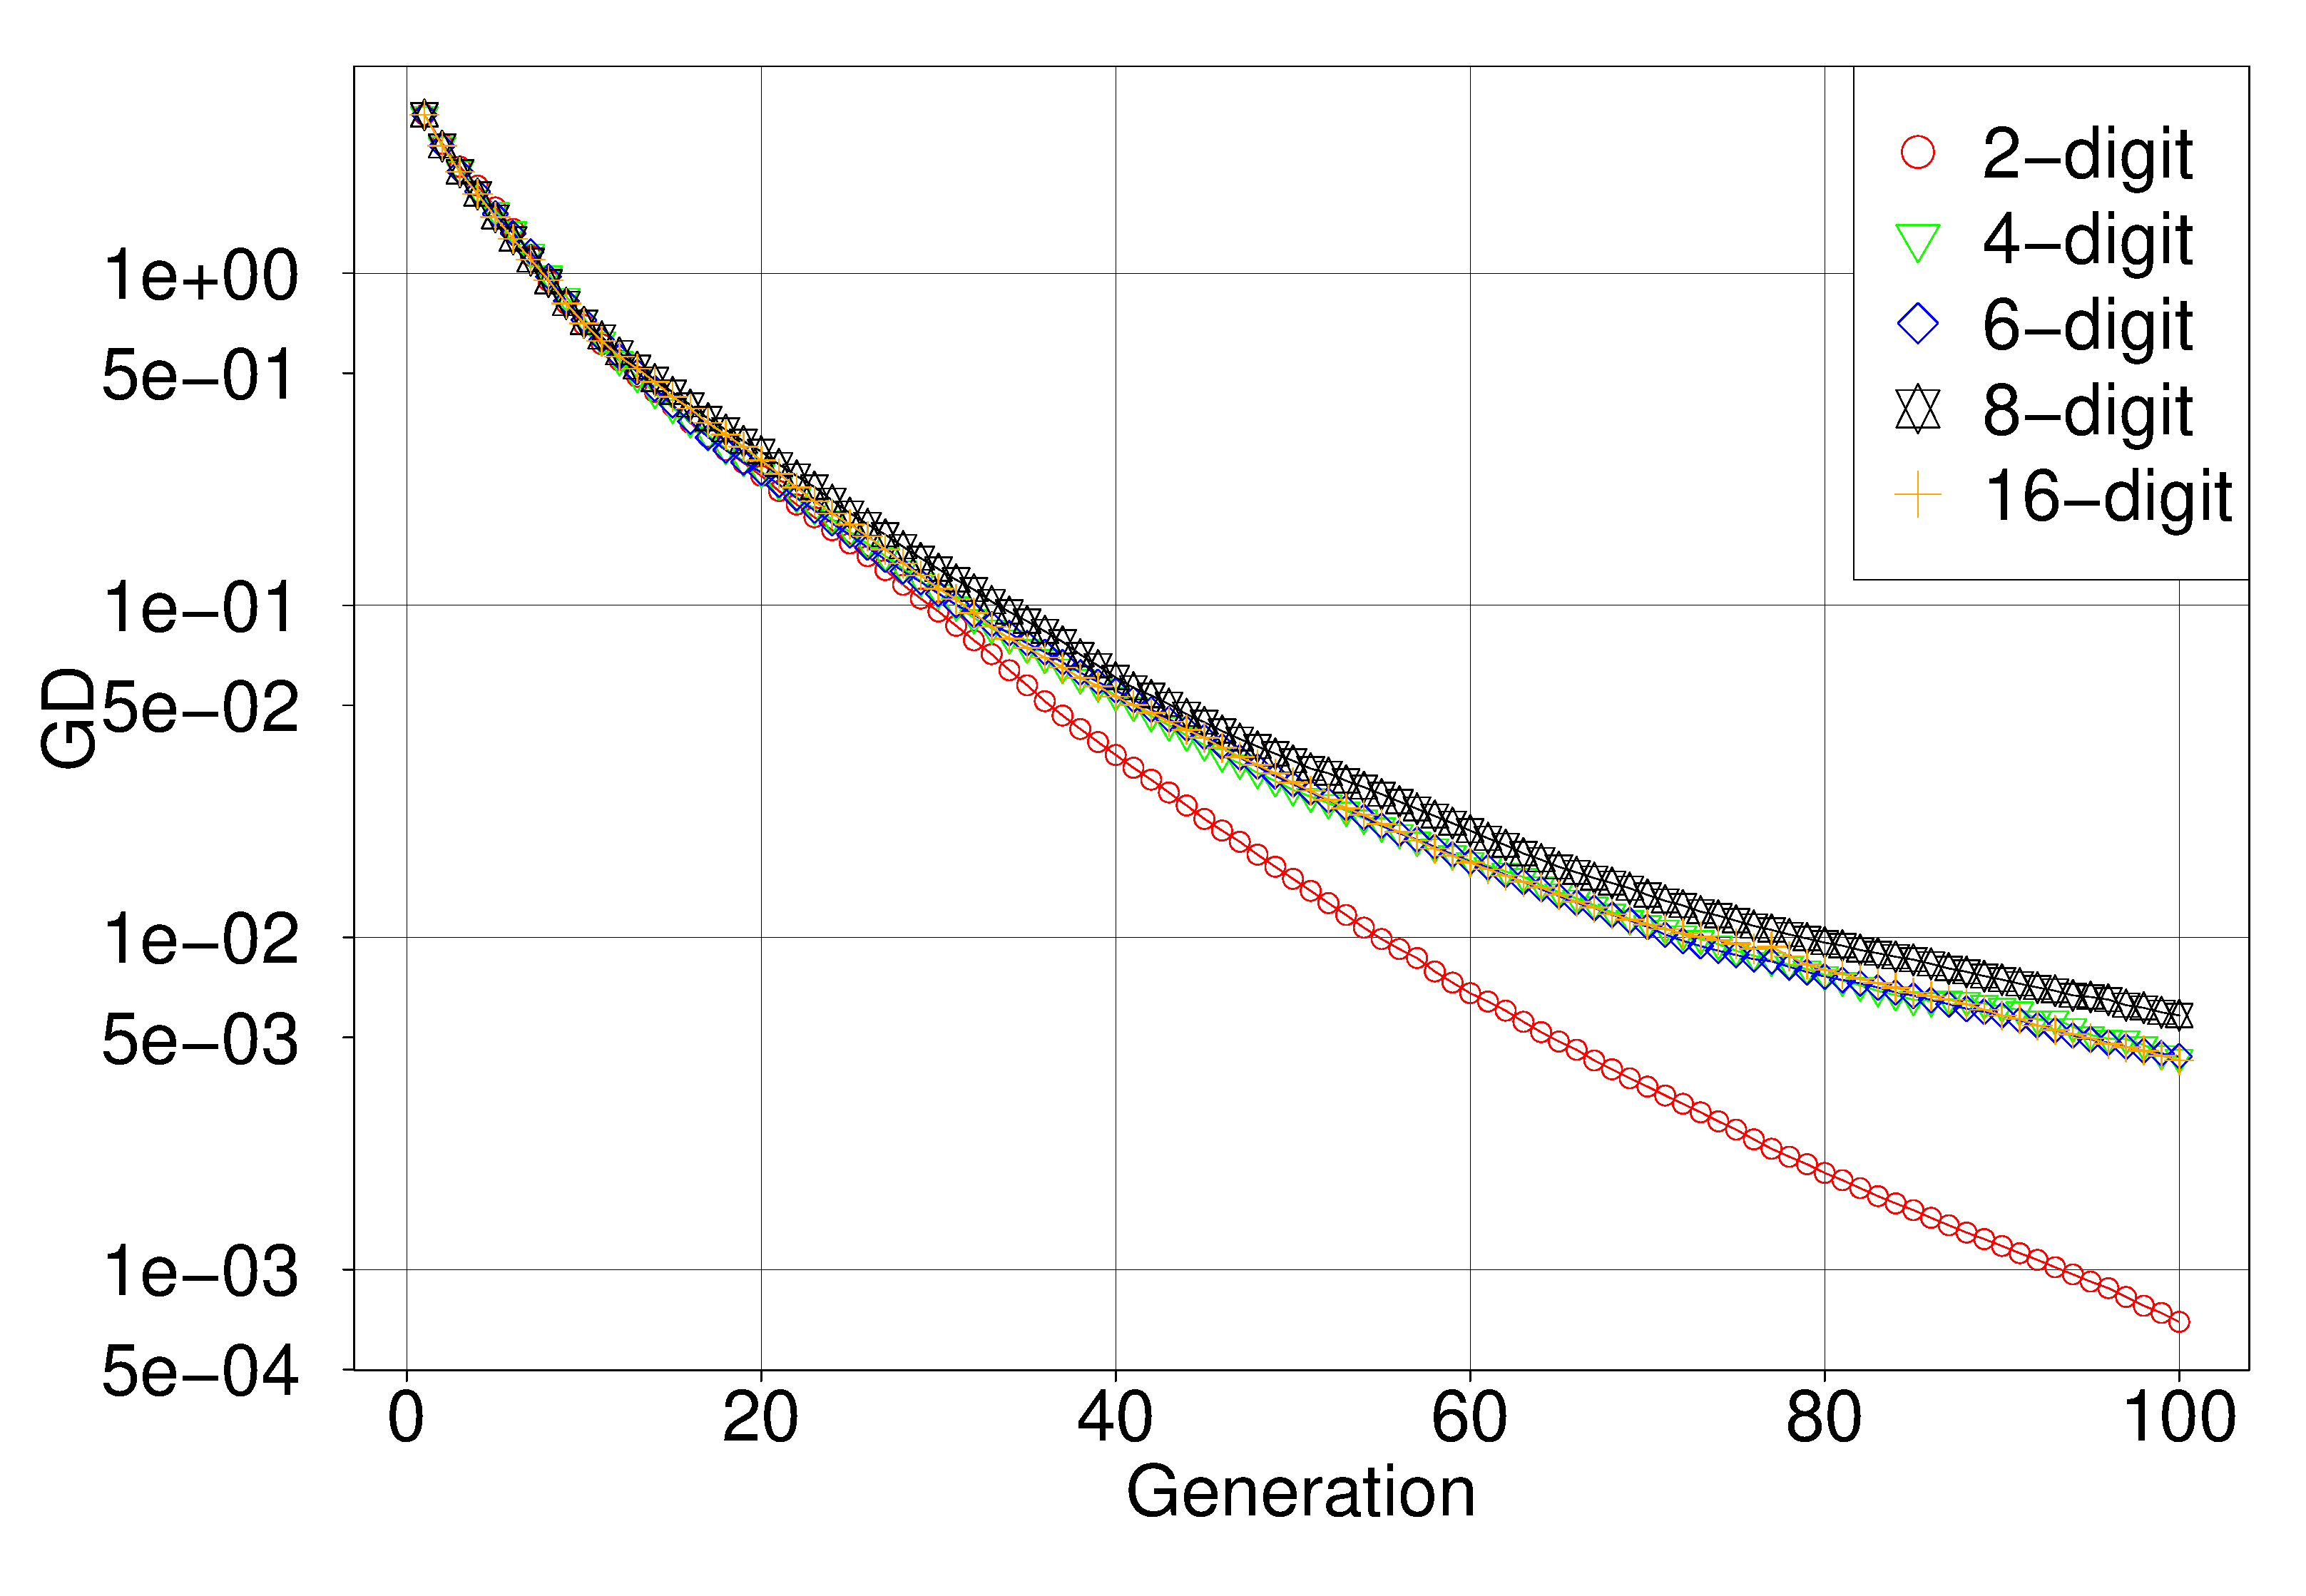
\includegraphics[width=1\linewidth]{../figures/MOEAD/DTLZ4_GD.eps}
\begin{center}
{\footnotesize (c) DTLZ4}
\end{center}
\end{minipage}
\end{tabular}
\caption{DTLZ2-4におけるGDの推移(MOEA/D)}
\label{fig:gd_dtlz_moead}
\end{figure*}

\begin{figure*}[htbp]
\begin{tabular}{cc}
\begin{minipage}{0.32\hsize}
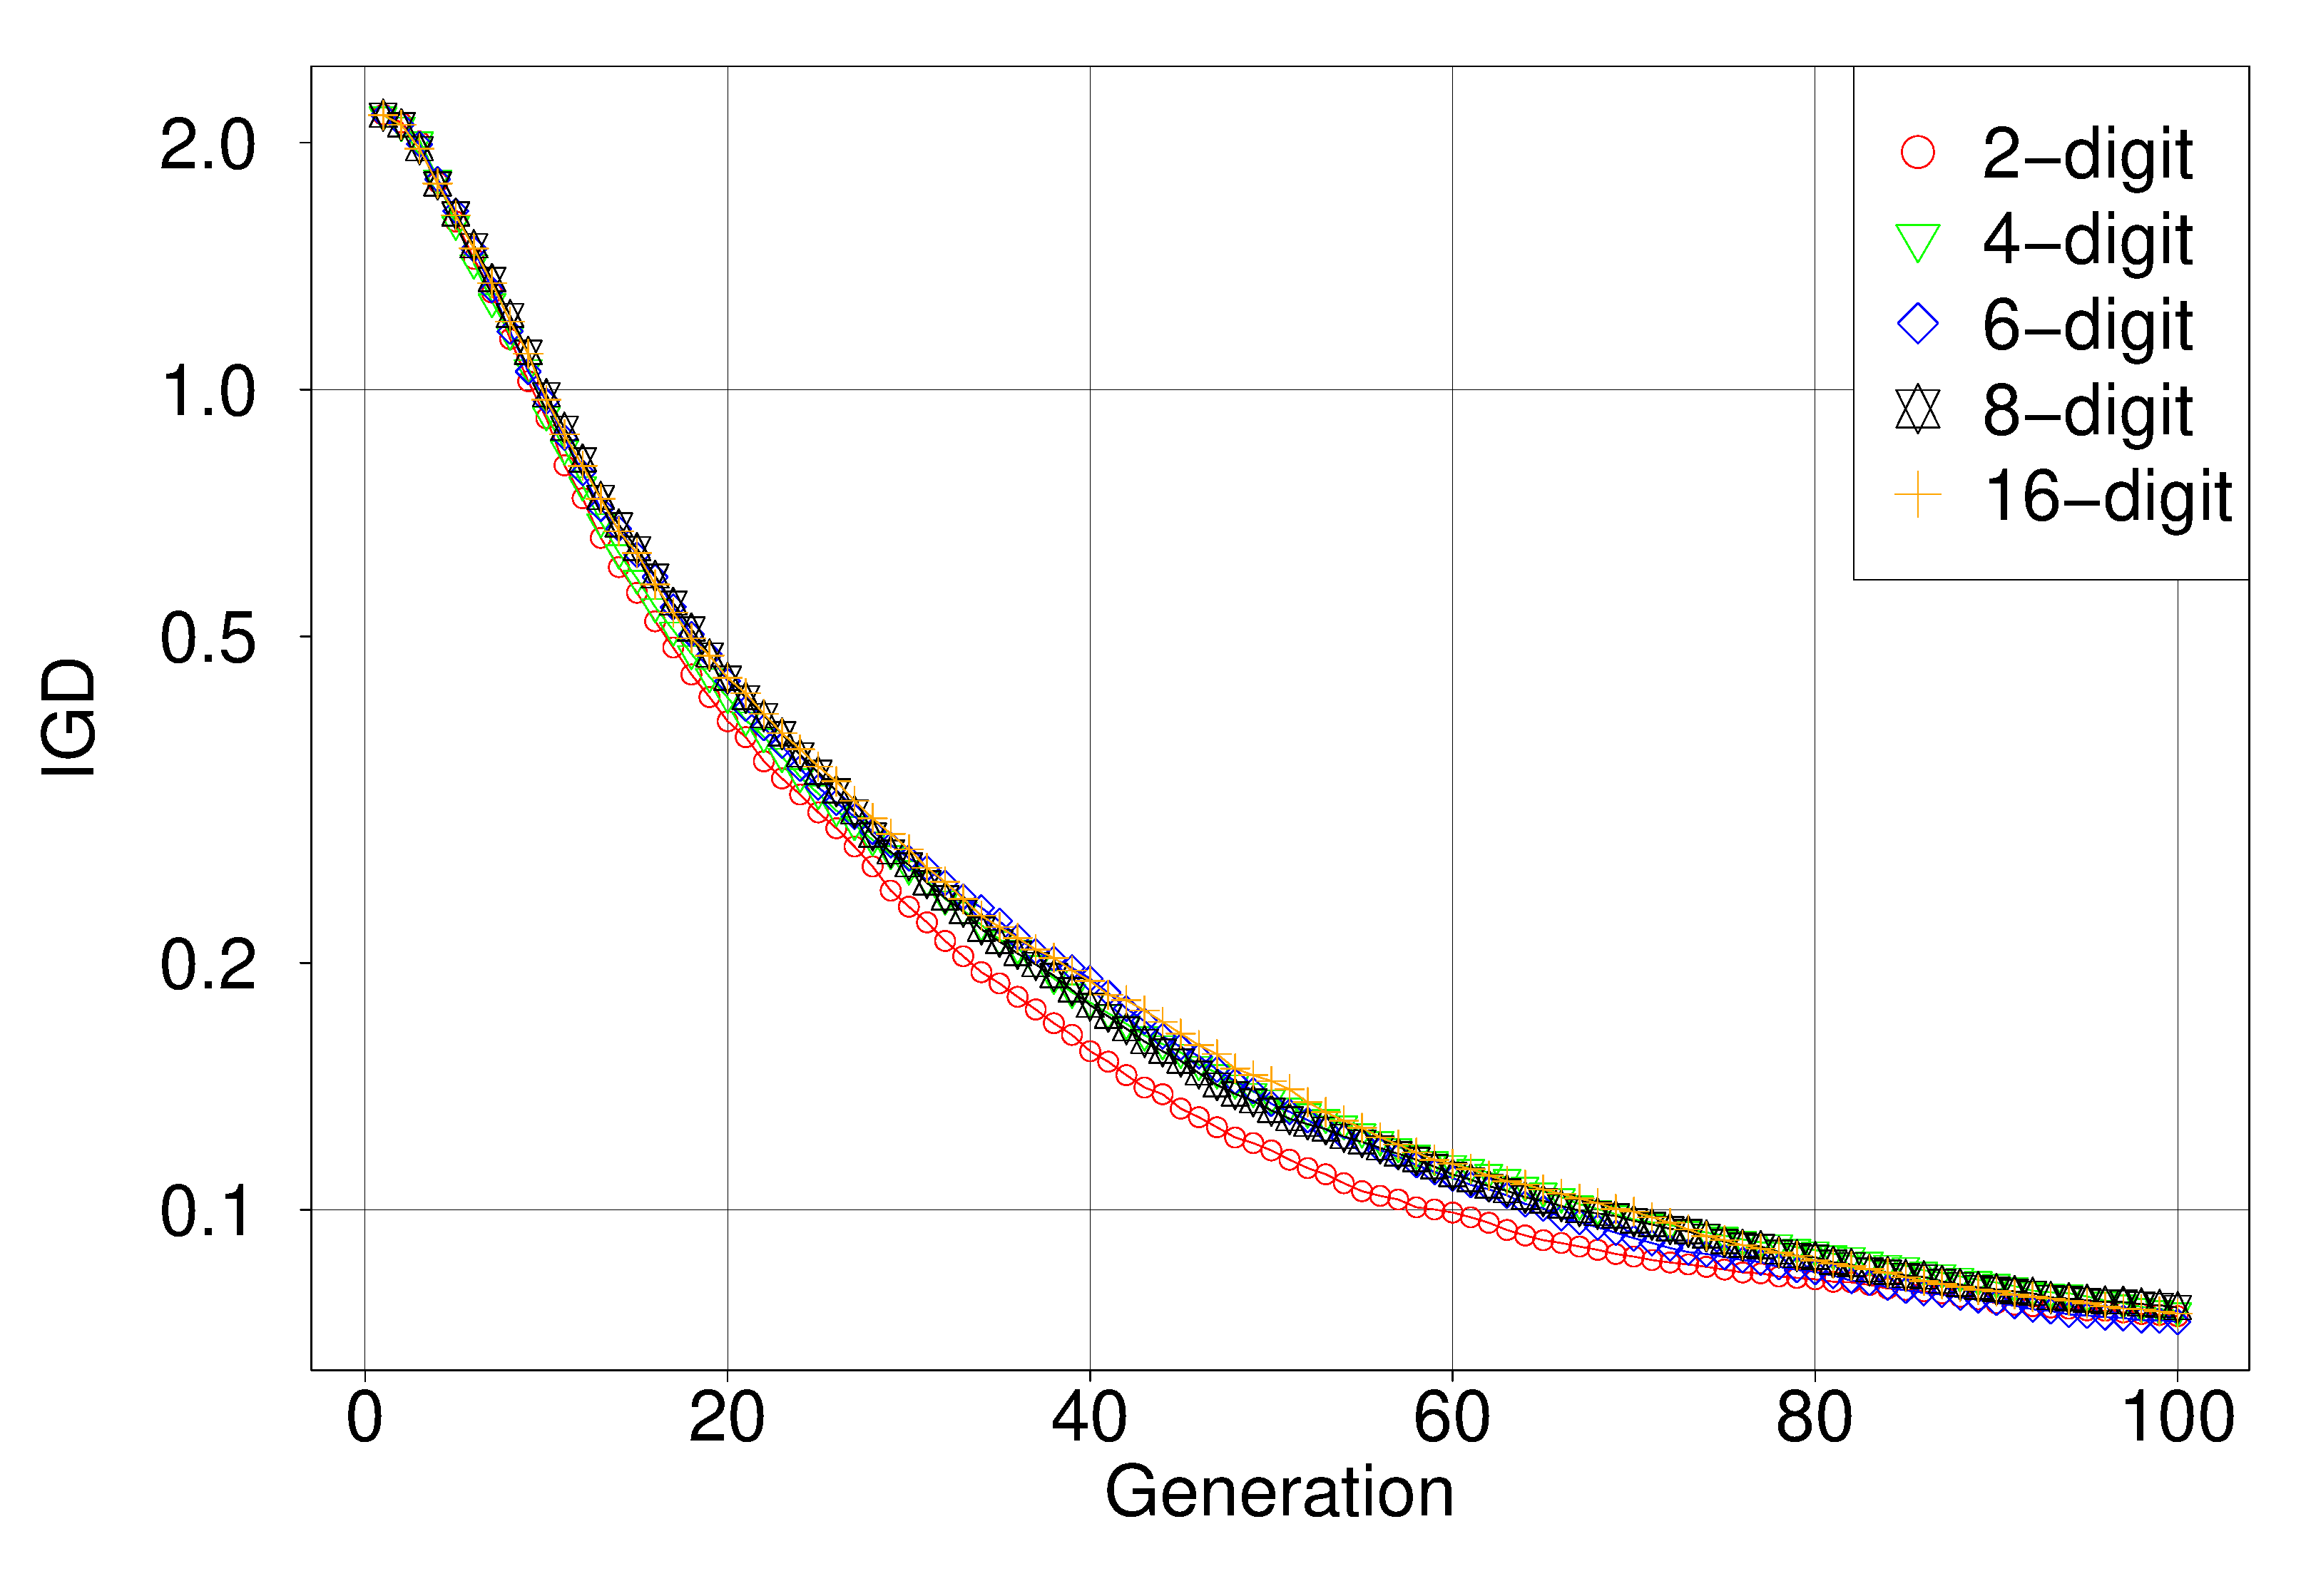
\includegraphics[width=1\linewidth]{../figures/MOEAD/DTLZ2_IGD.eps}
\begin{center}
{\footnotesize (a) DTLZ2}
\end{center}
\end{minipage}
\begin{minipage}{0.32\hsize}
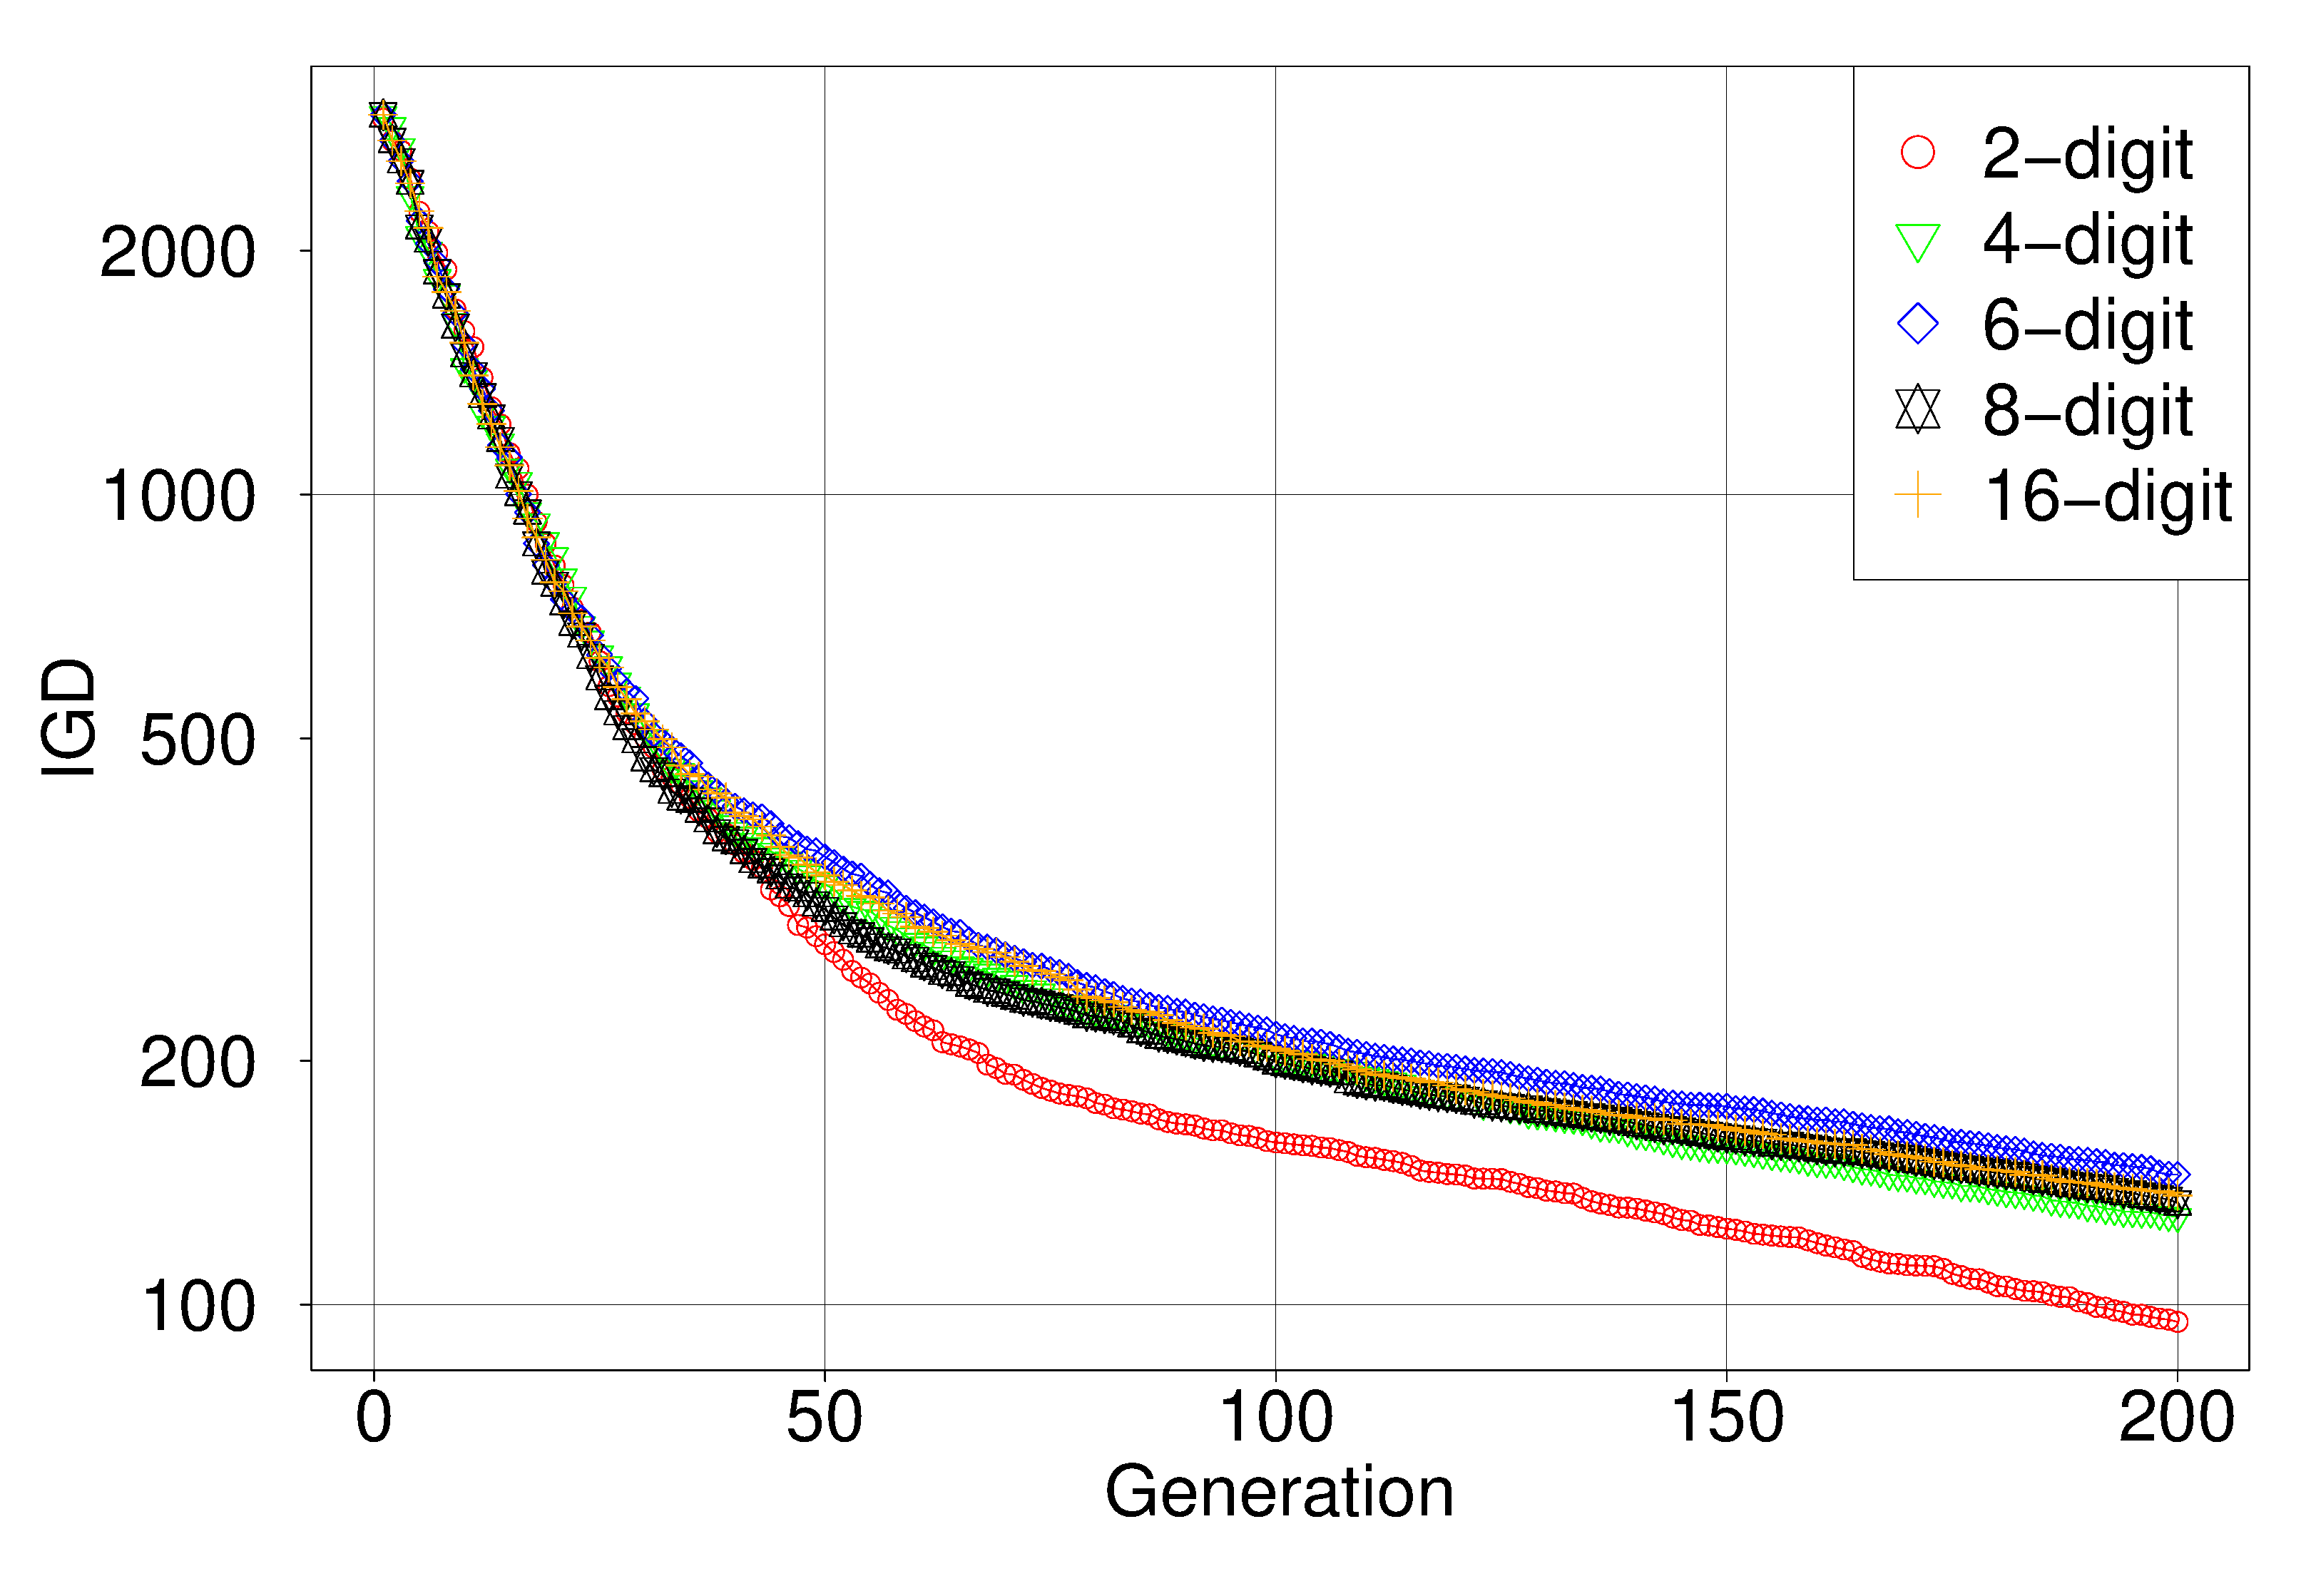
\includegraphics[width=1\linewidth]{../figures/MOEAD/DTLZ3_IGD.eps}
\begin{center}
{\footnotesize (b) DTLZ3}
\end{center}
\end{minipage}
\begin{minipage}{0.32\hsize}
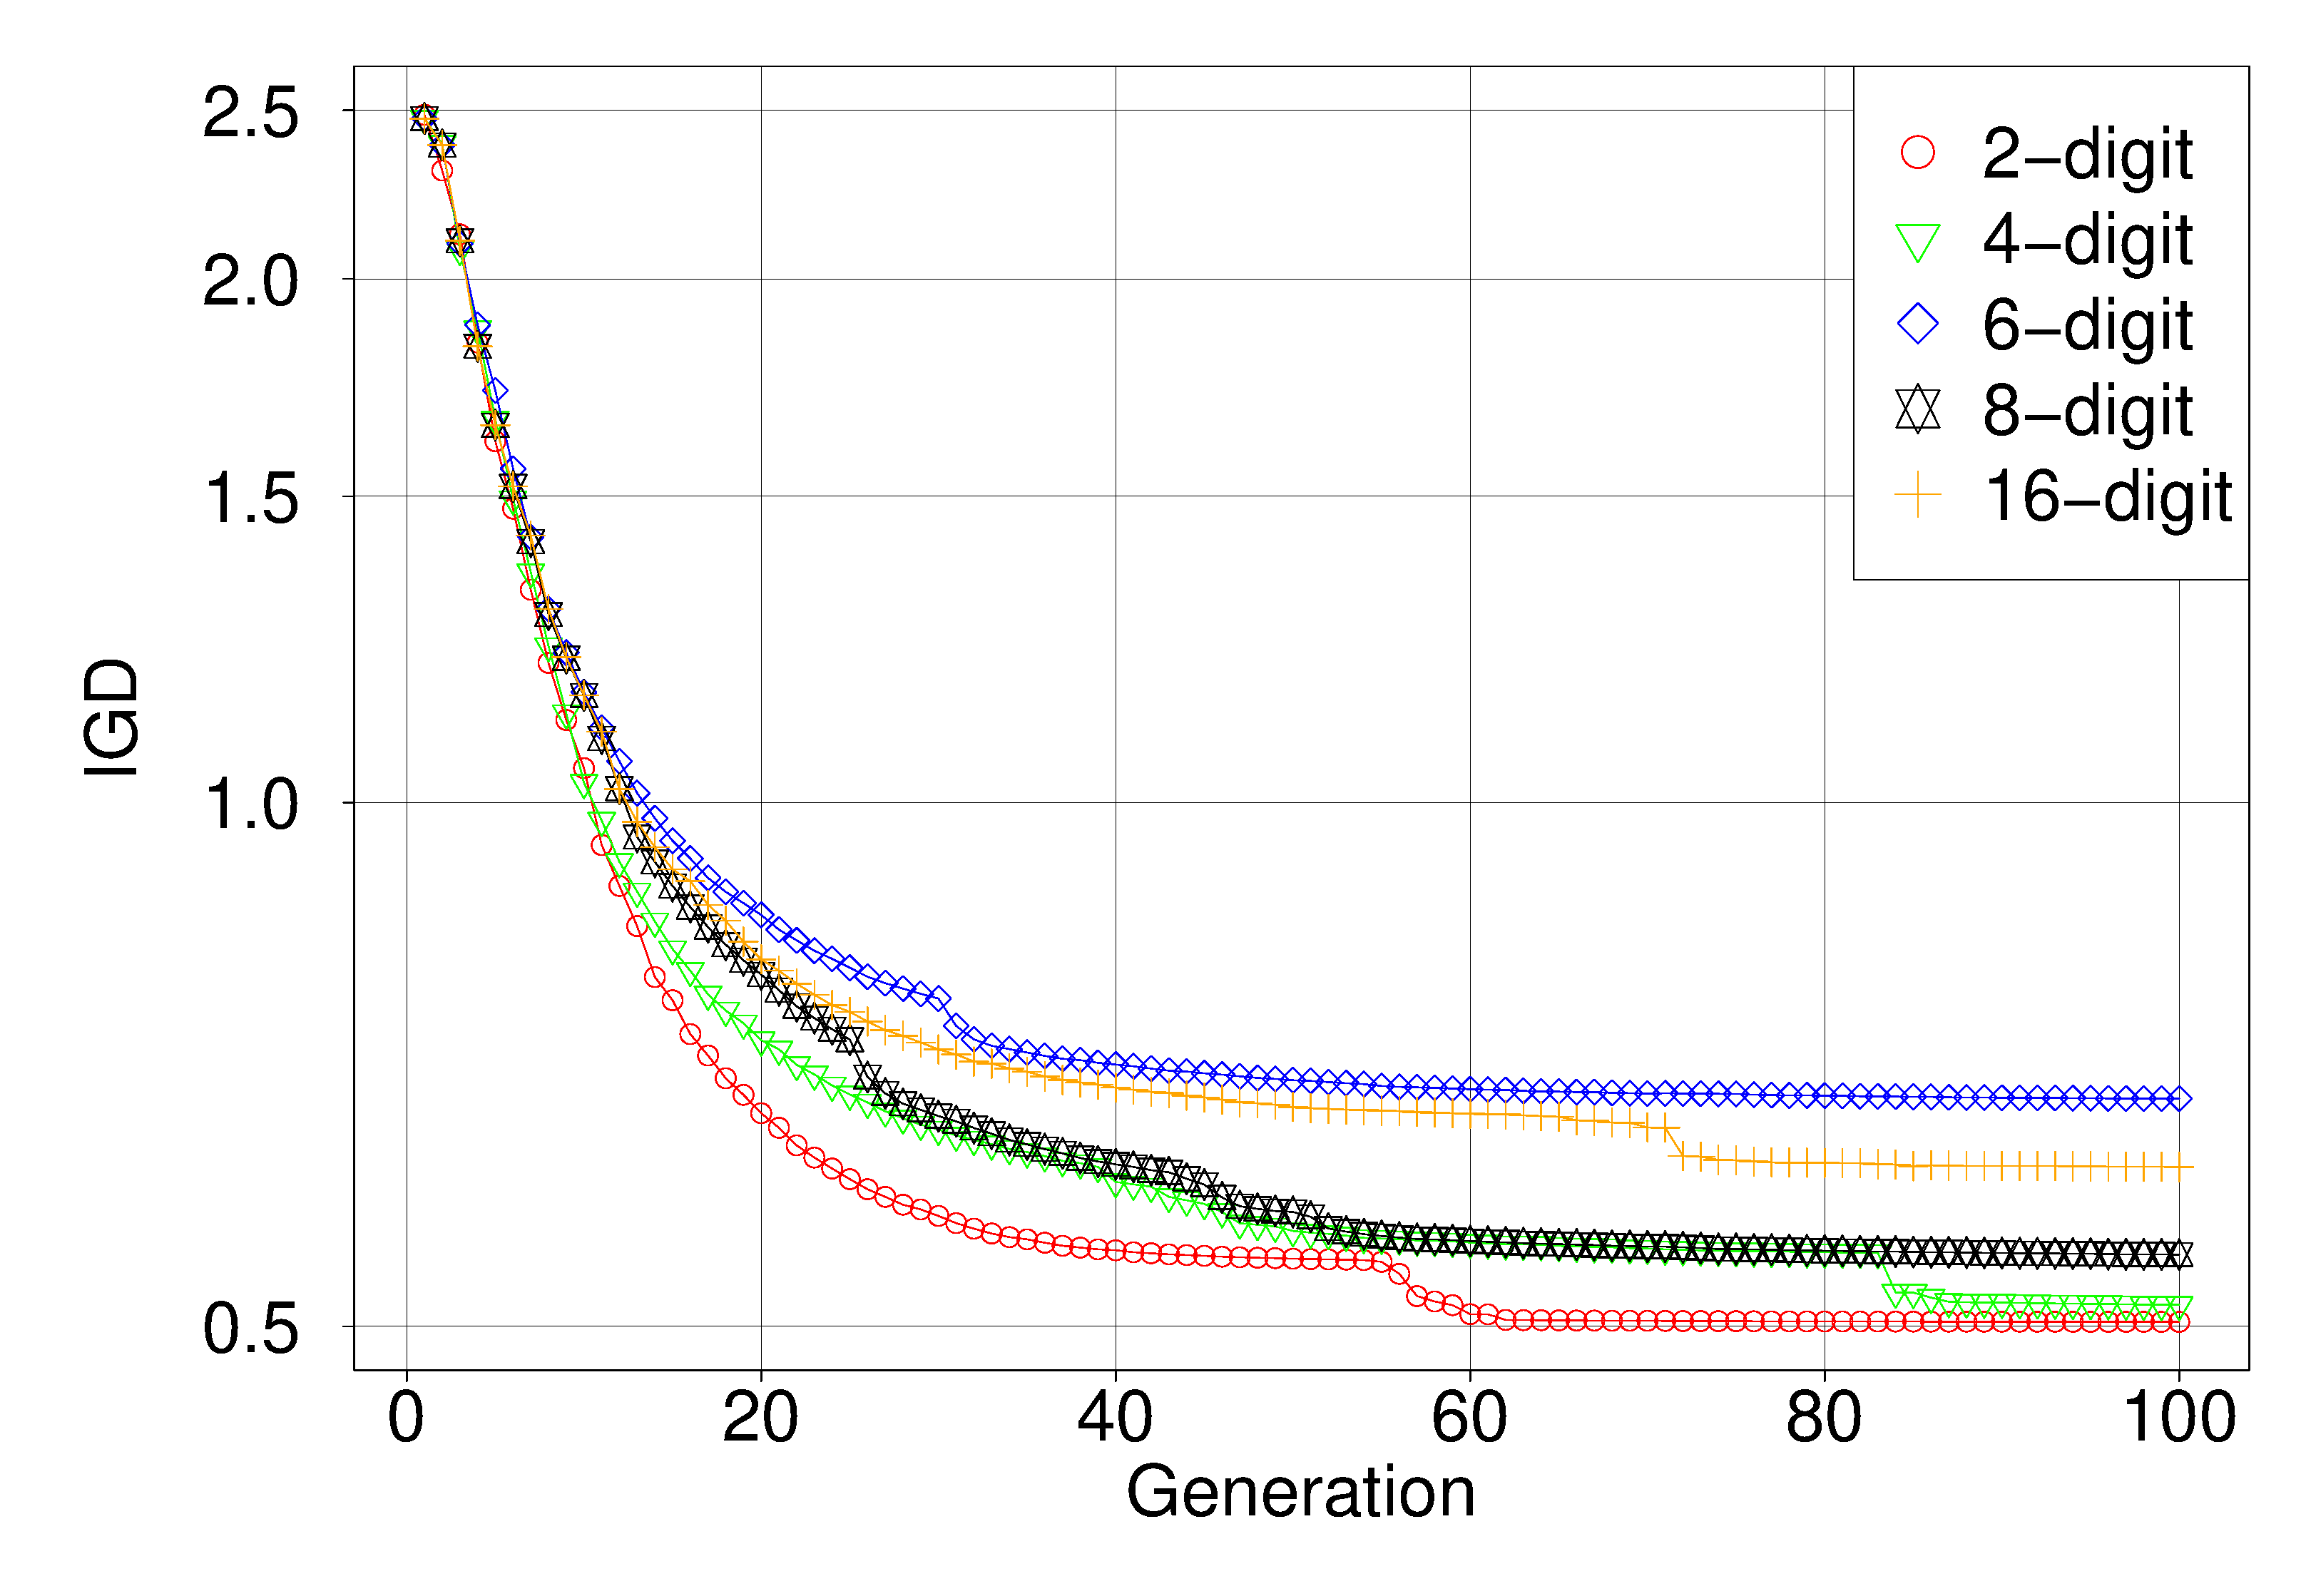
\includegraphics[width=1\linewidth]{../figures/MOEAD/DTLZ4_IGD.eps}
\begin{center}
{\footnotesize (c) DTLZ4}
\end{center}
\end{minipage}
\end{tabular}
\caption{DTLZ2-4におけるIGDの推移(MOEA/D)}
\label{fig:igd_dtlz_moead}
\end{figure*}

\begin{figure*}[htbp]
\begin{tabular}{cc}
\begin{minipage}{0.32\hsize}
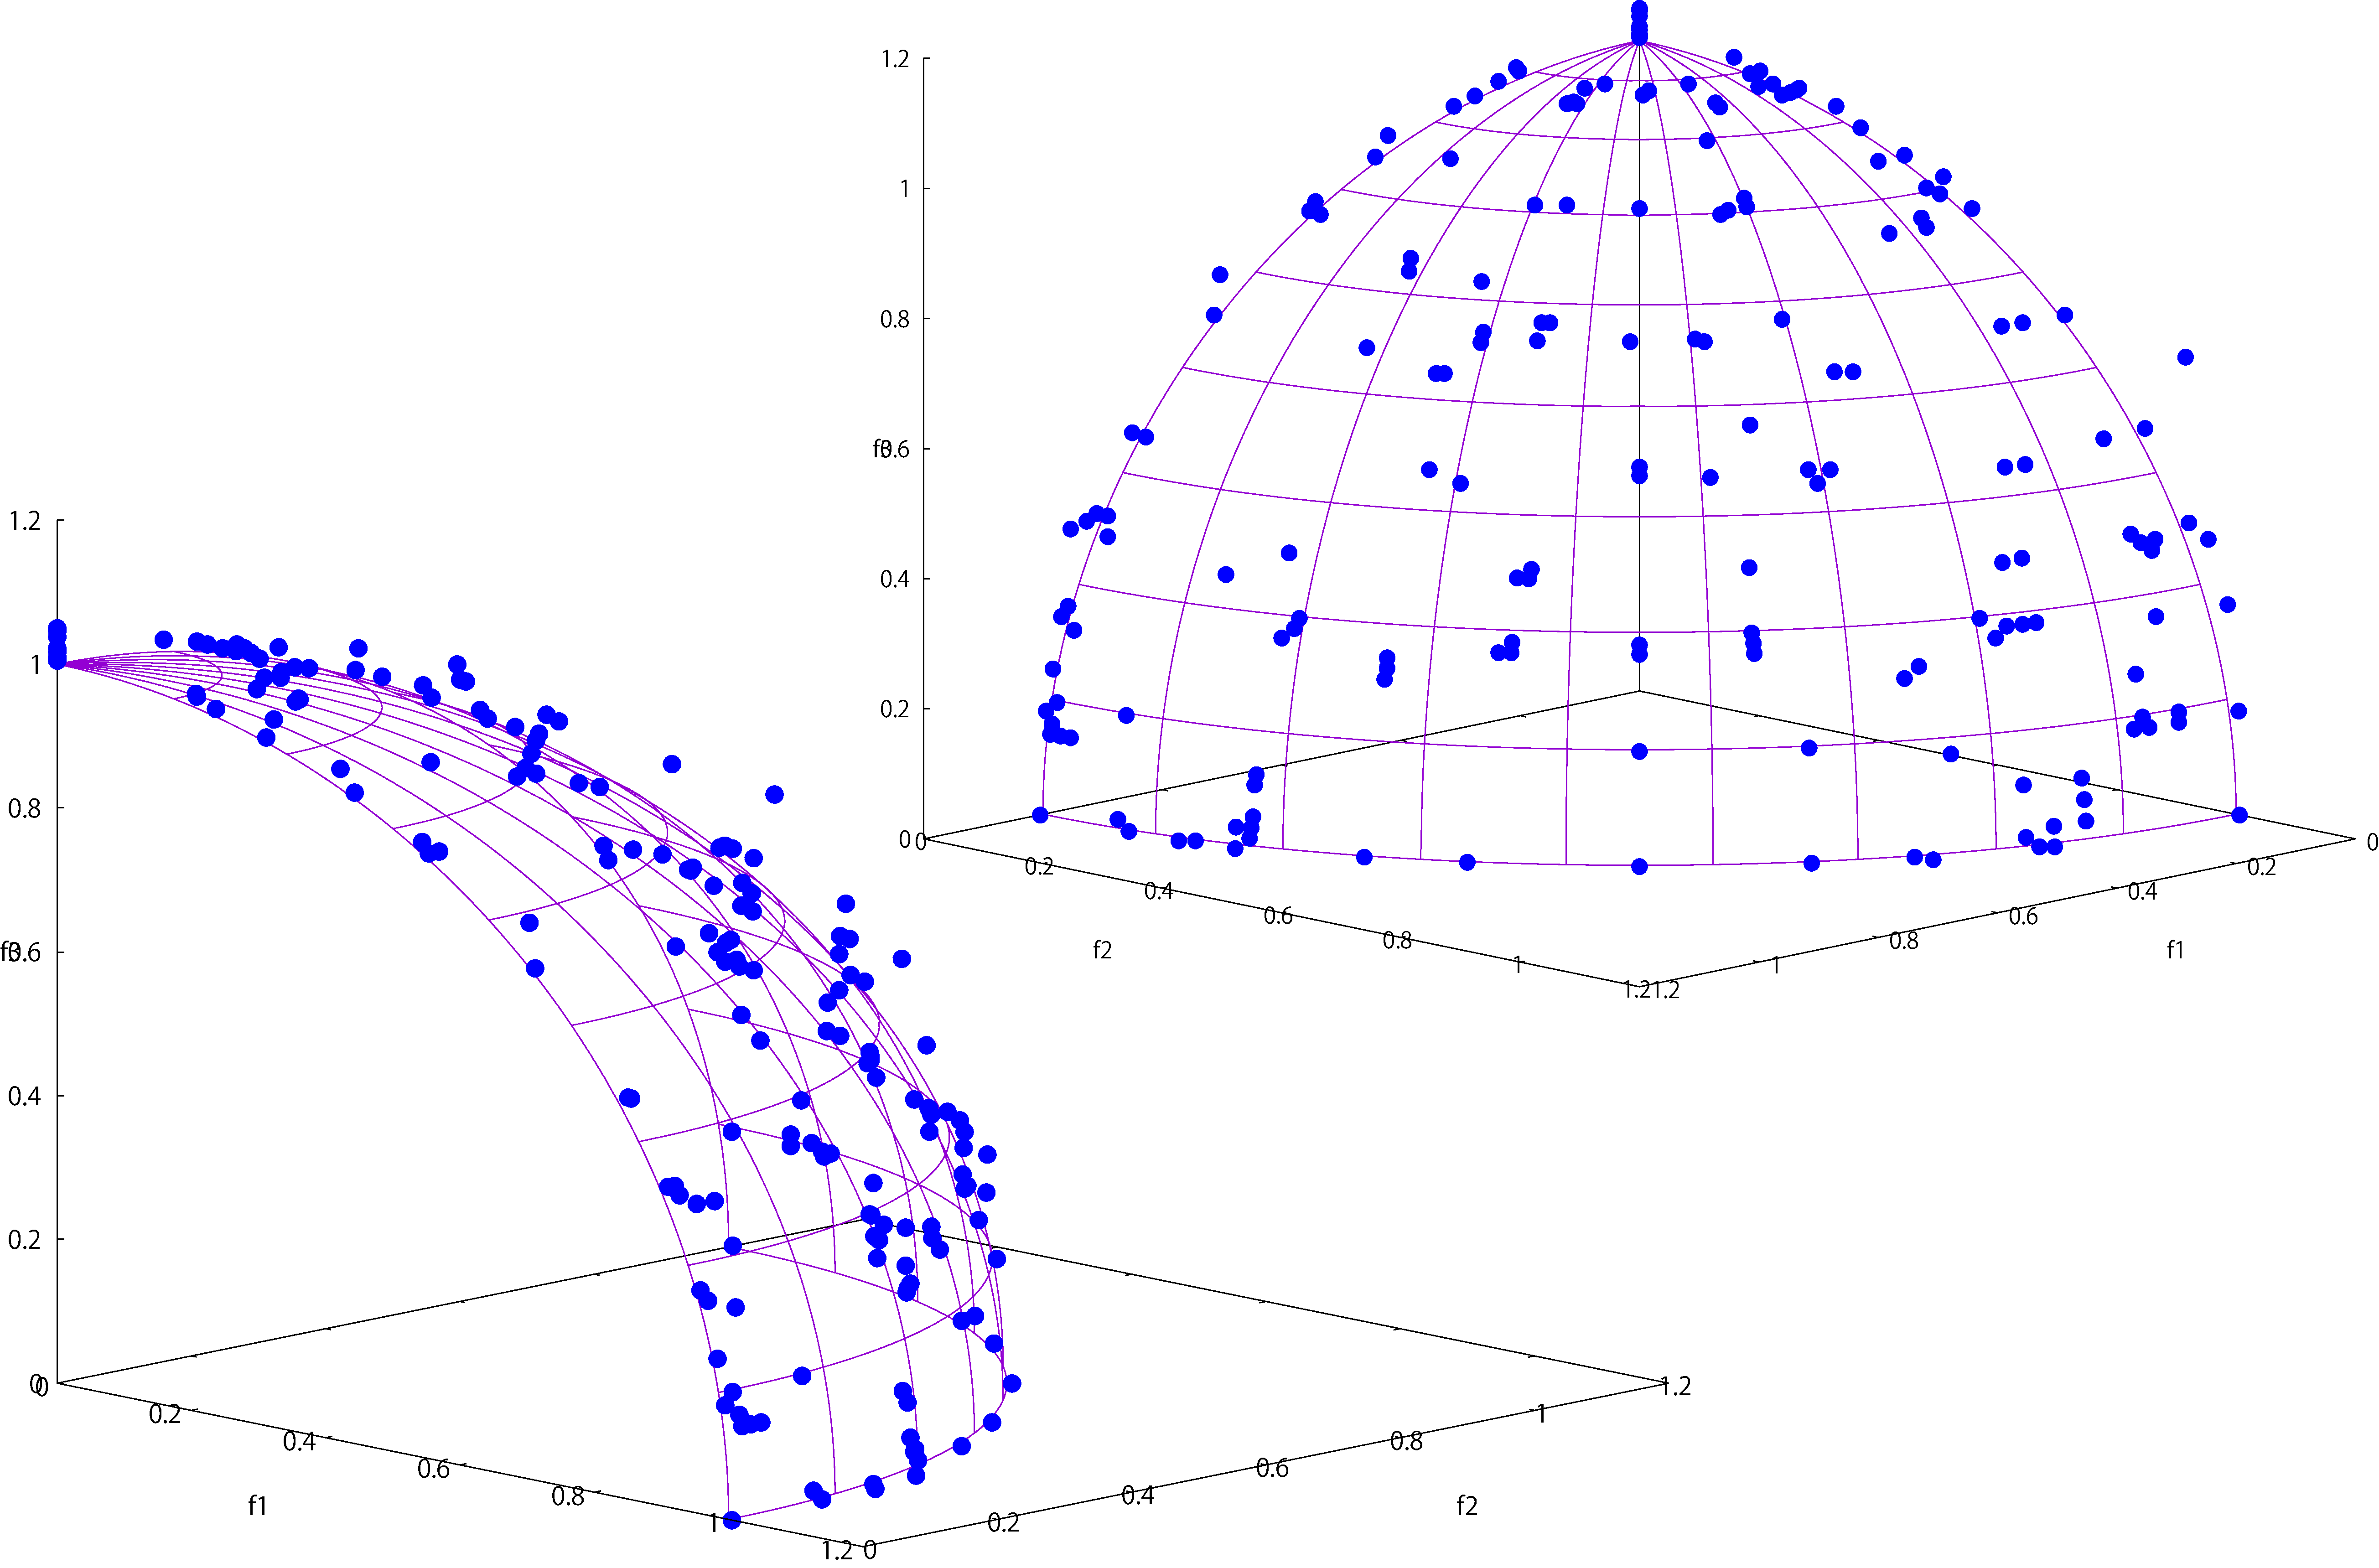
\includegraphics[width=1\linewidth]{../figures/MOEAD/DTLZ2_digi2_double.pdf}
\begin{center}
{\footnotesize (a) 2-digit resolution}
\end{center}
\end{minipage}
\begin{minipage}{0.32\hsize}
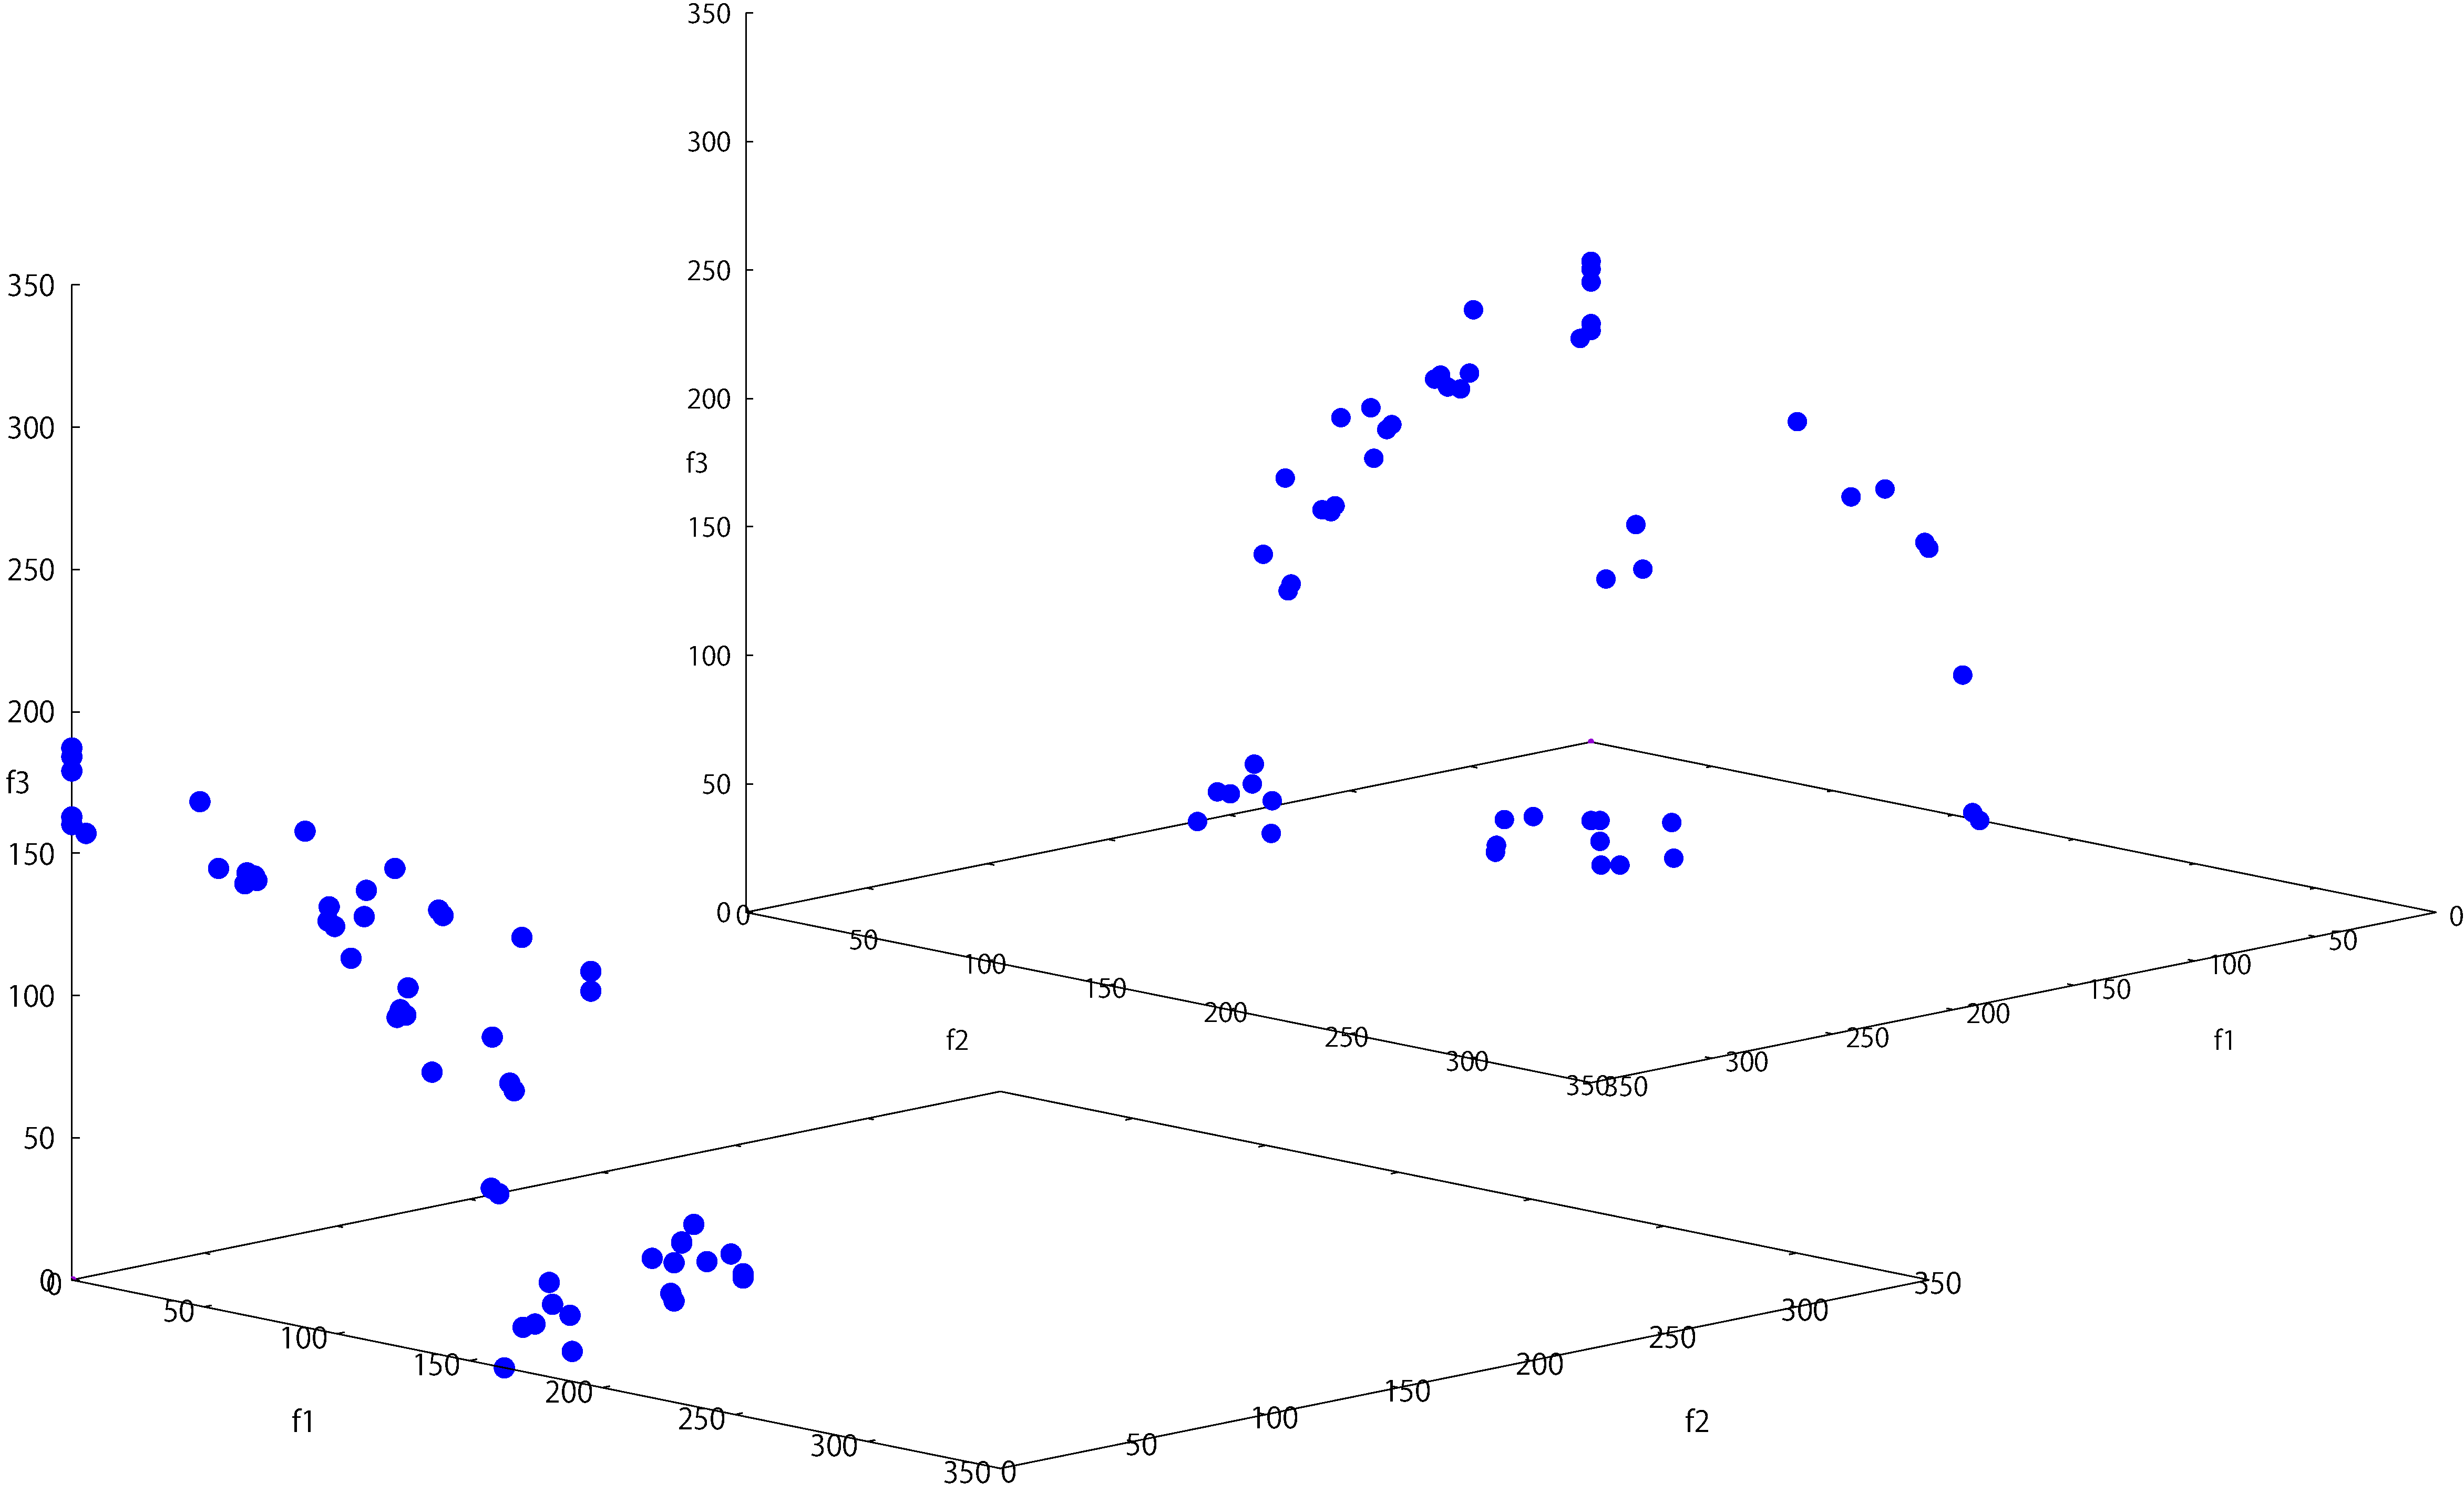
\includegraphics[width=1\linewidth]{../figures/MOEAD/DTLZ3_digi2_double.pdf}
\begin{center}
{\footnotesize (a) 2-digit resolution}
\end{center}
\end{minipage}
\begin{minipage}{0.32\hsize}
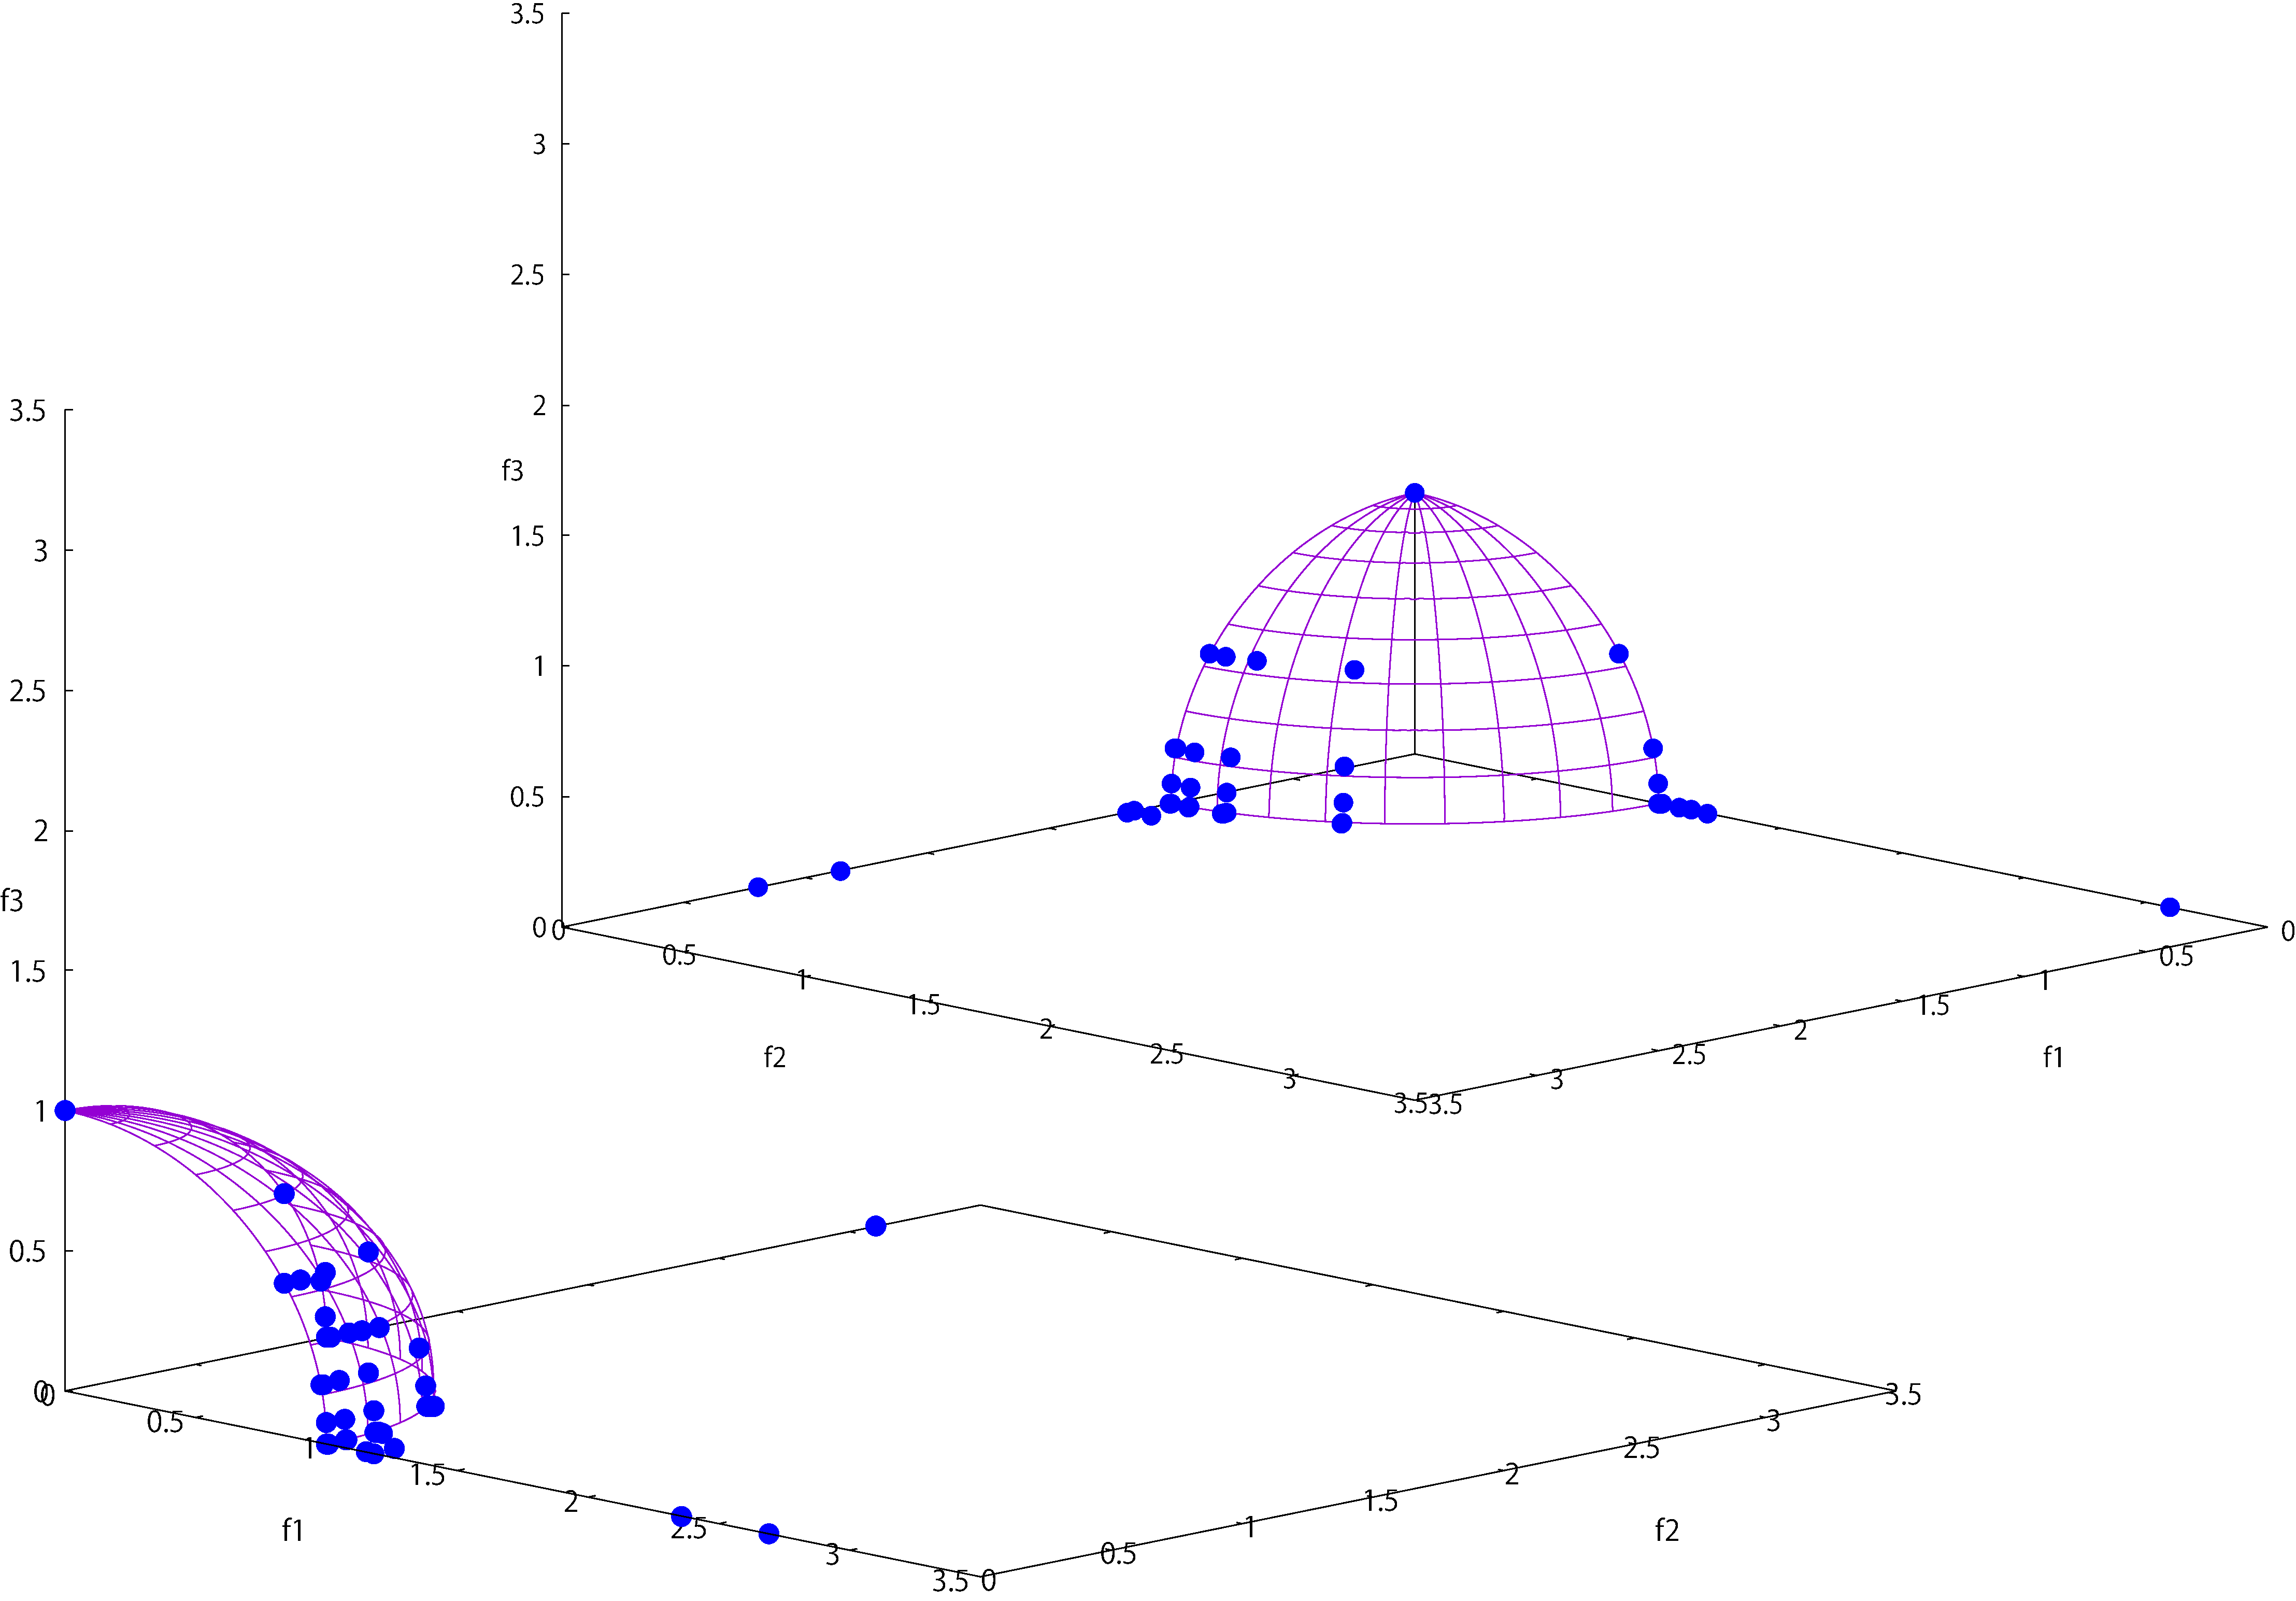
\includegraphics[width=1\linewidth]{../figures/MOEAD/DTLZ4_digi2_double.pdf}
\begin{center}
{\footnotesize (a) 2-digit resolution}
\end{center}
\end{minipage}
\end{tabular}
%\label{fig:dtlz4}
\end{figure*}

\begin{figure*}[!htbp]
\begin{tabular}{cc}
\begin{minipage}{0.32\hsize}
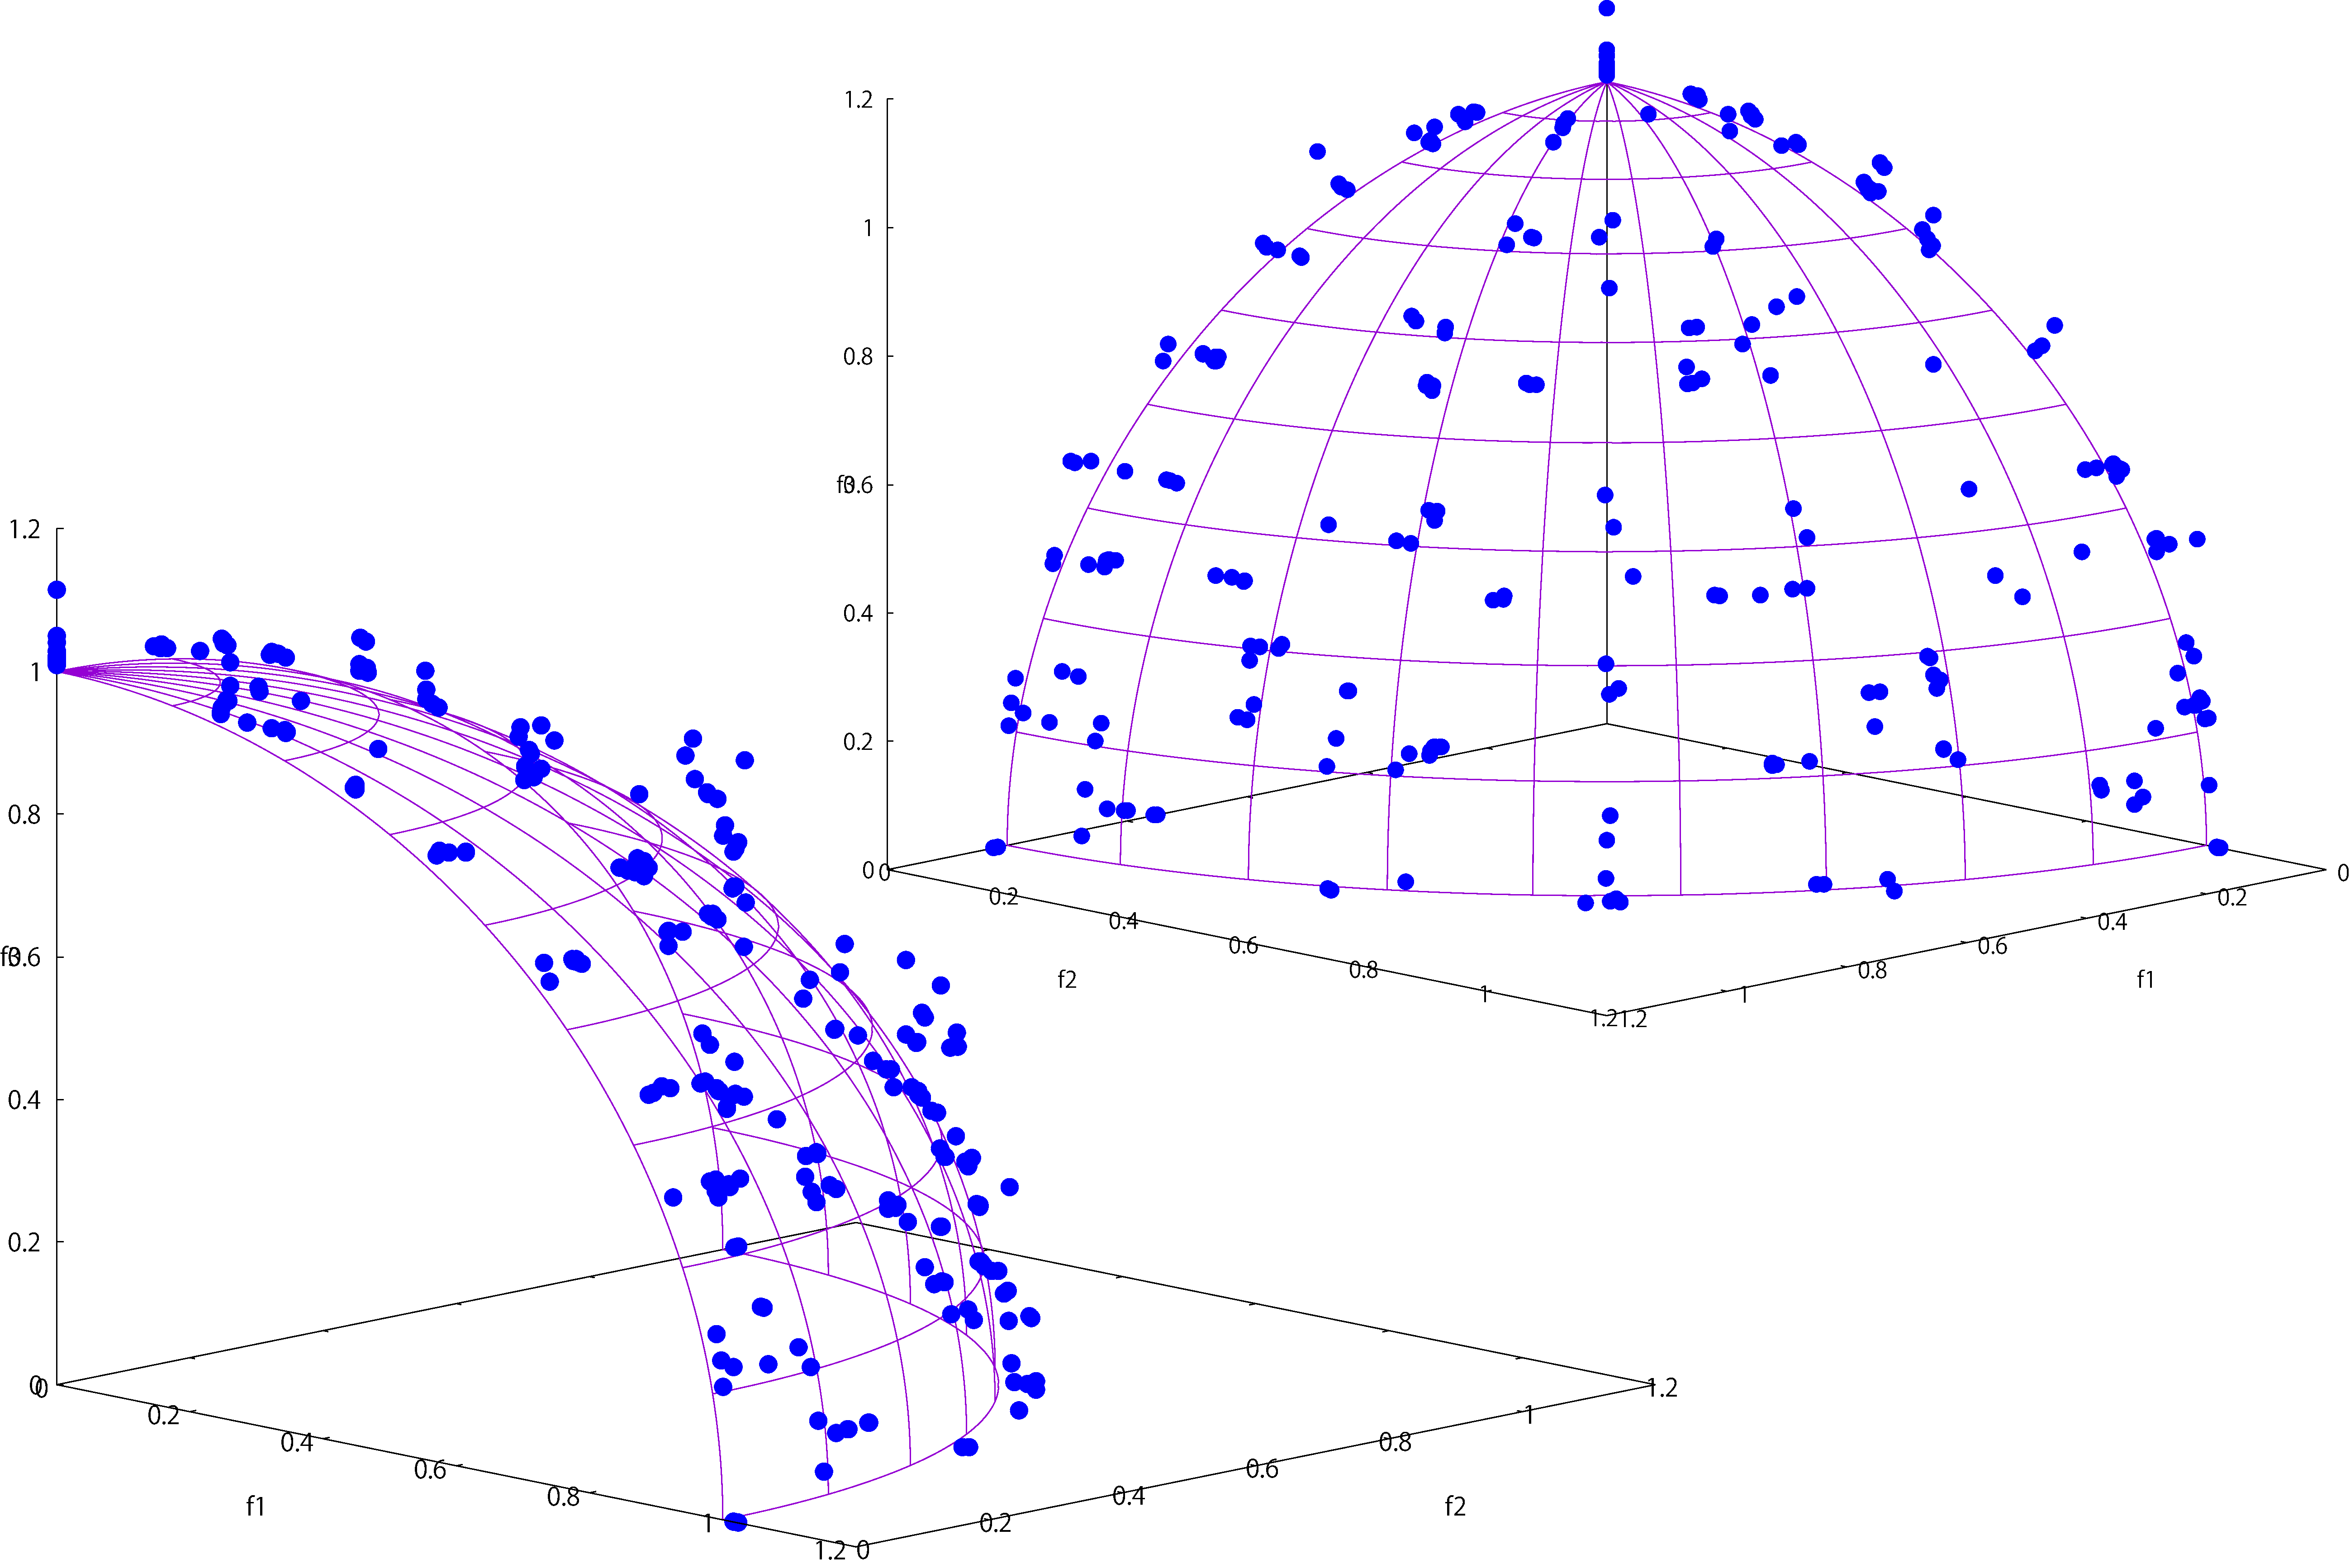
\includegraphics[width=1\linewidth]{../figures/MOEAD/DTLZ2_digi16_double.pdf}
\centering
%\begin{center}
{\footnotesize (b) 16-digit resolution}
\caption{DTLZ2における非劣解の分布(MOEA/D)}
\label{ogawaku--n}
%\end{center}
\end{minipage}
\begin{minipage}{0.32\hsize}
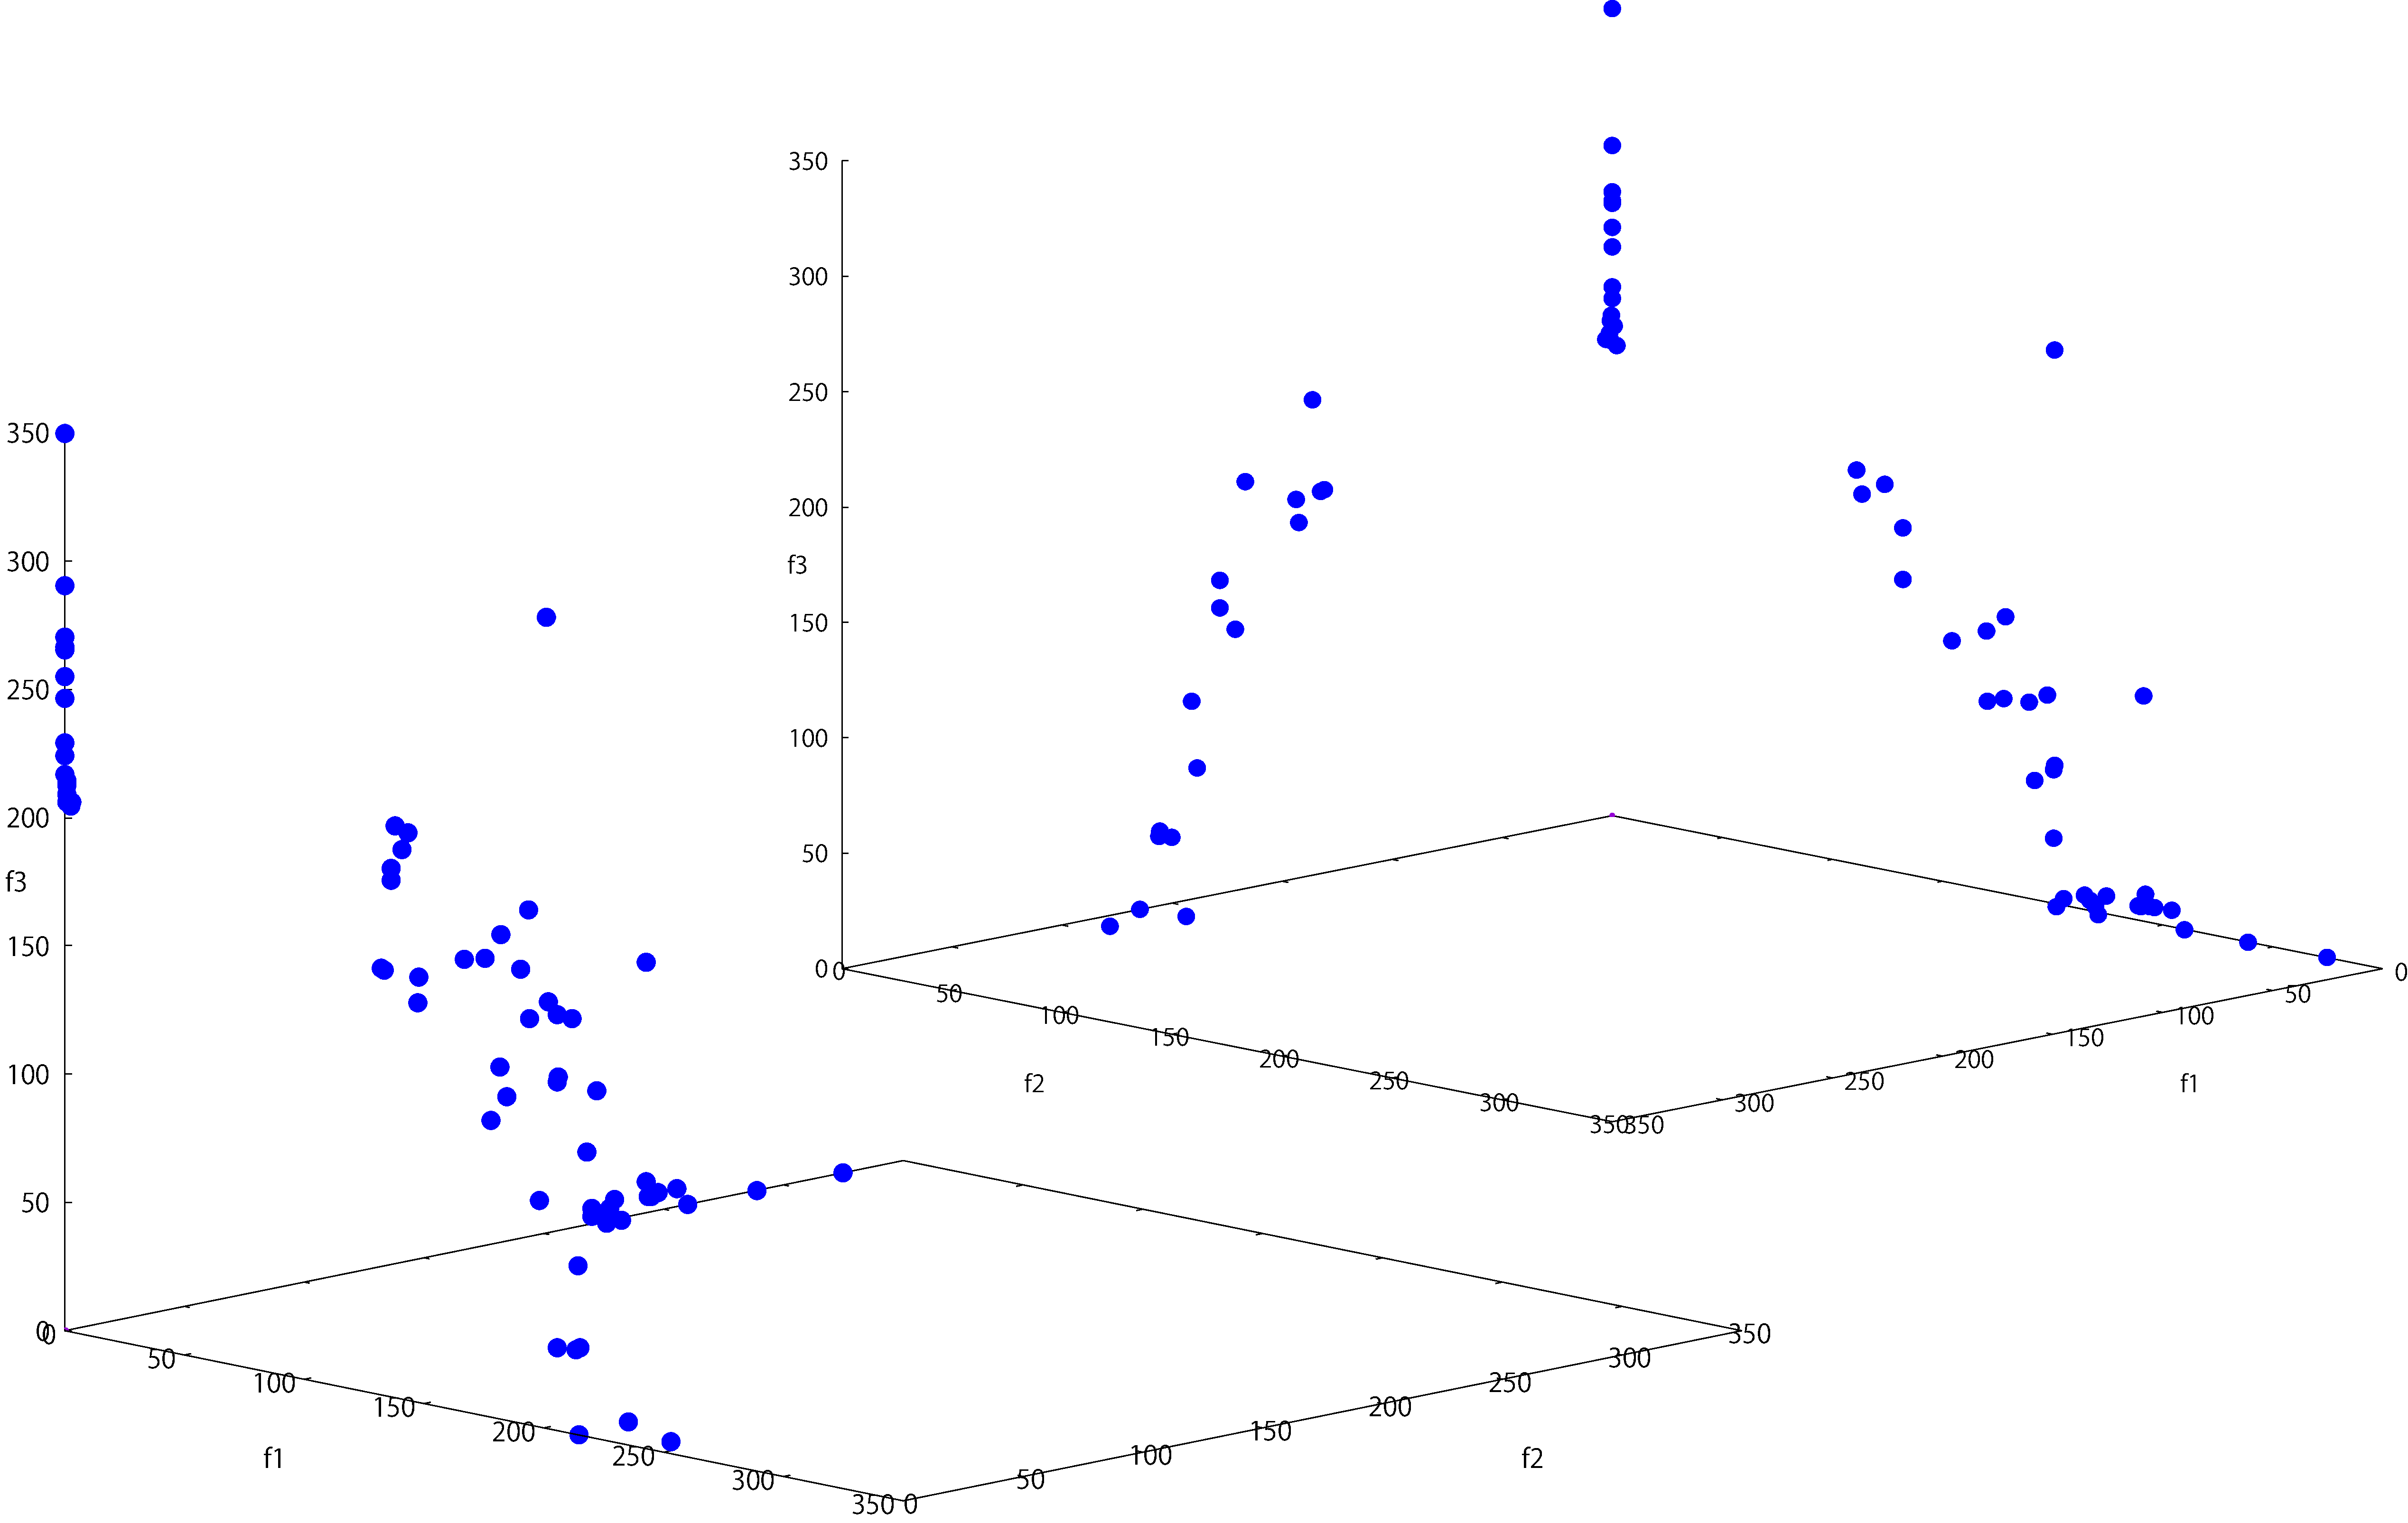
\includegraphics[width=1\linewidth]{../figures/MOEAD/DTLZ3_digi16_double.pdf}
\centering
{\footnotesize (b) 16-digit resolution}
\caption{DTLZ3における非劣解の分布(MOEA/D)}
\label{kondouku--n}
\end{minipage}
\begin{minipage}{0.32\hsize}
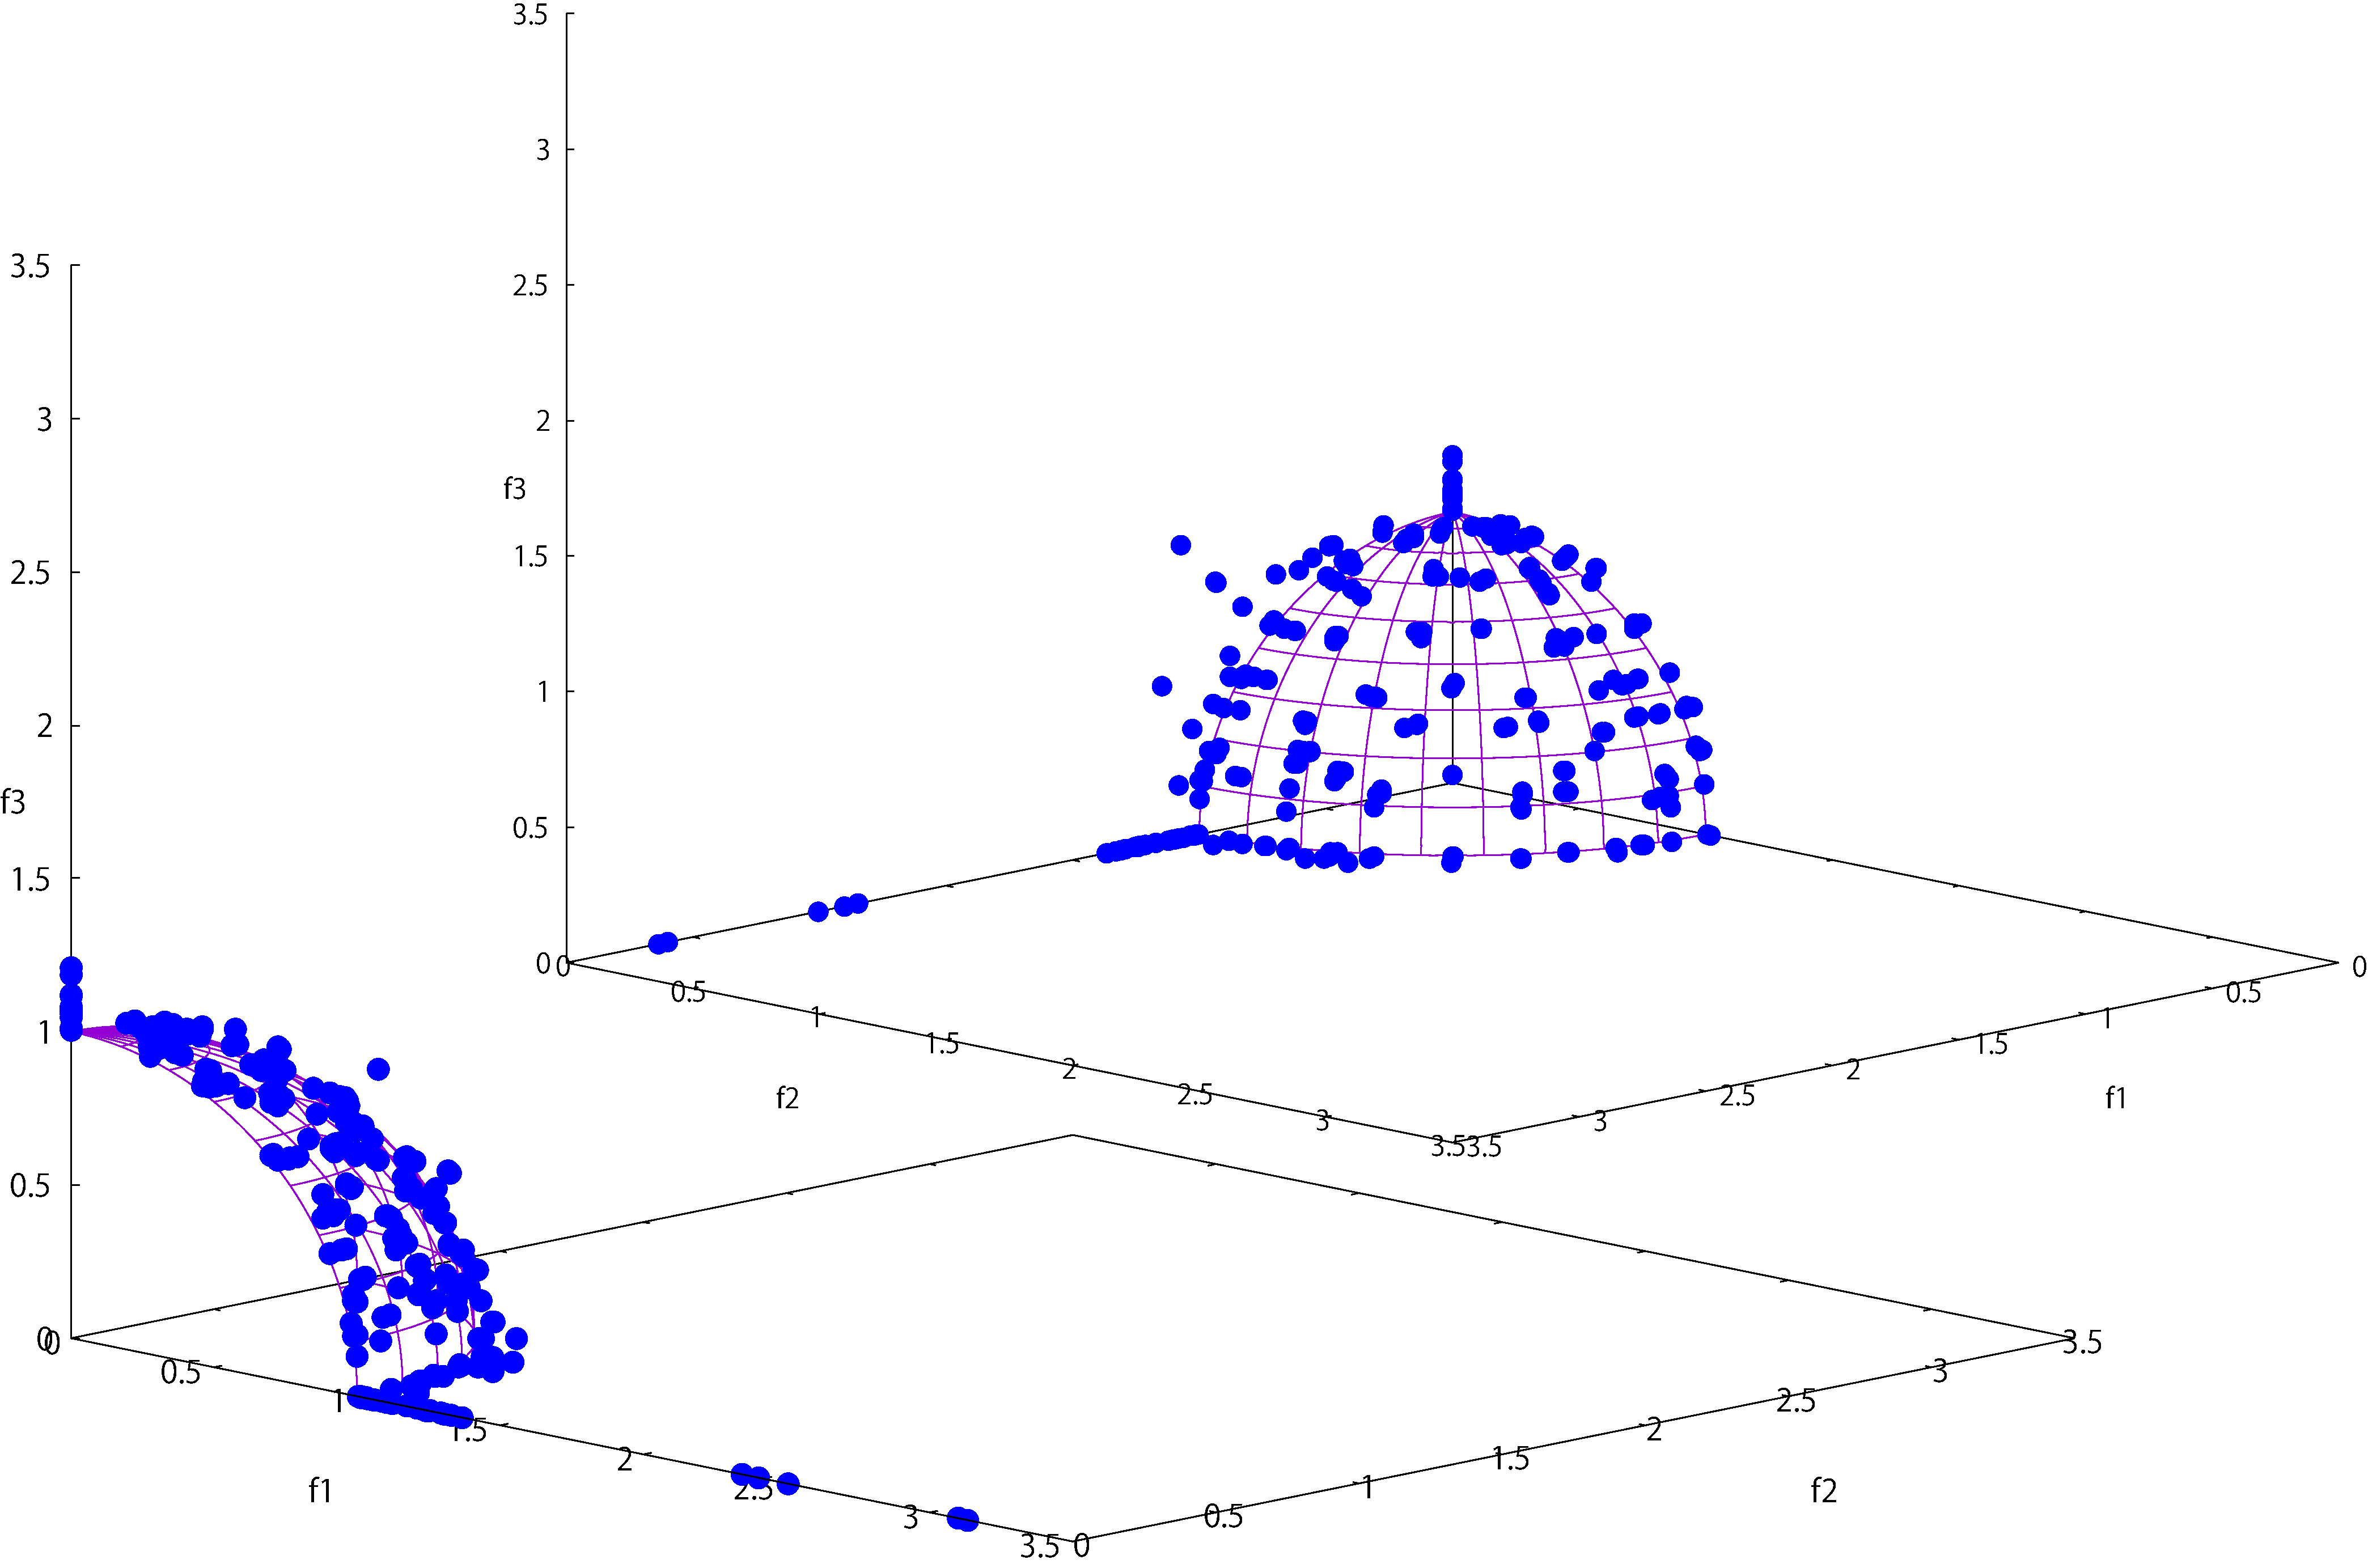
\includegraphics[width=1\linewidth]{../figures/MOEAD/DTLZ4_digi16_double.pdf}
\centering
{\footnotesize (b) 16-digit resolution}
\caption{DTLZ4における非劣解の分布(MOEA/D)}
\label{katorisa--n}
\end{minipage}
\end{tabular}
\end{figure*}

\begin{figure*}[htbp]
\begin{tabular}{cc}
\begin{minipage}{0.32\hsize}
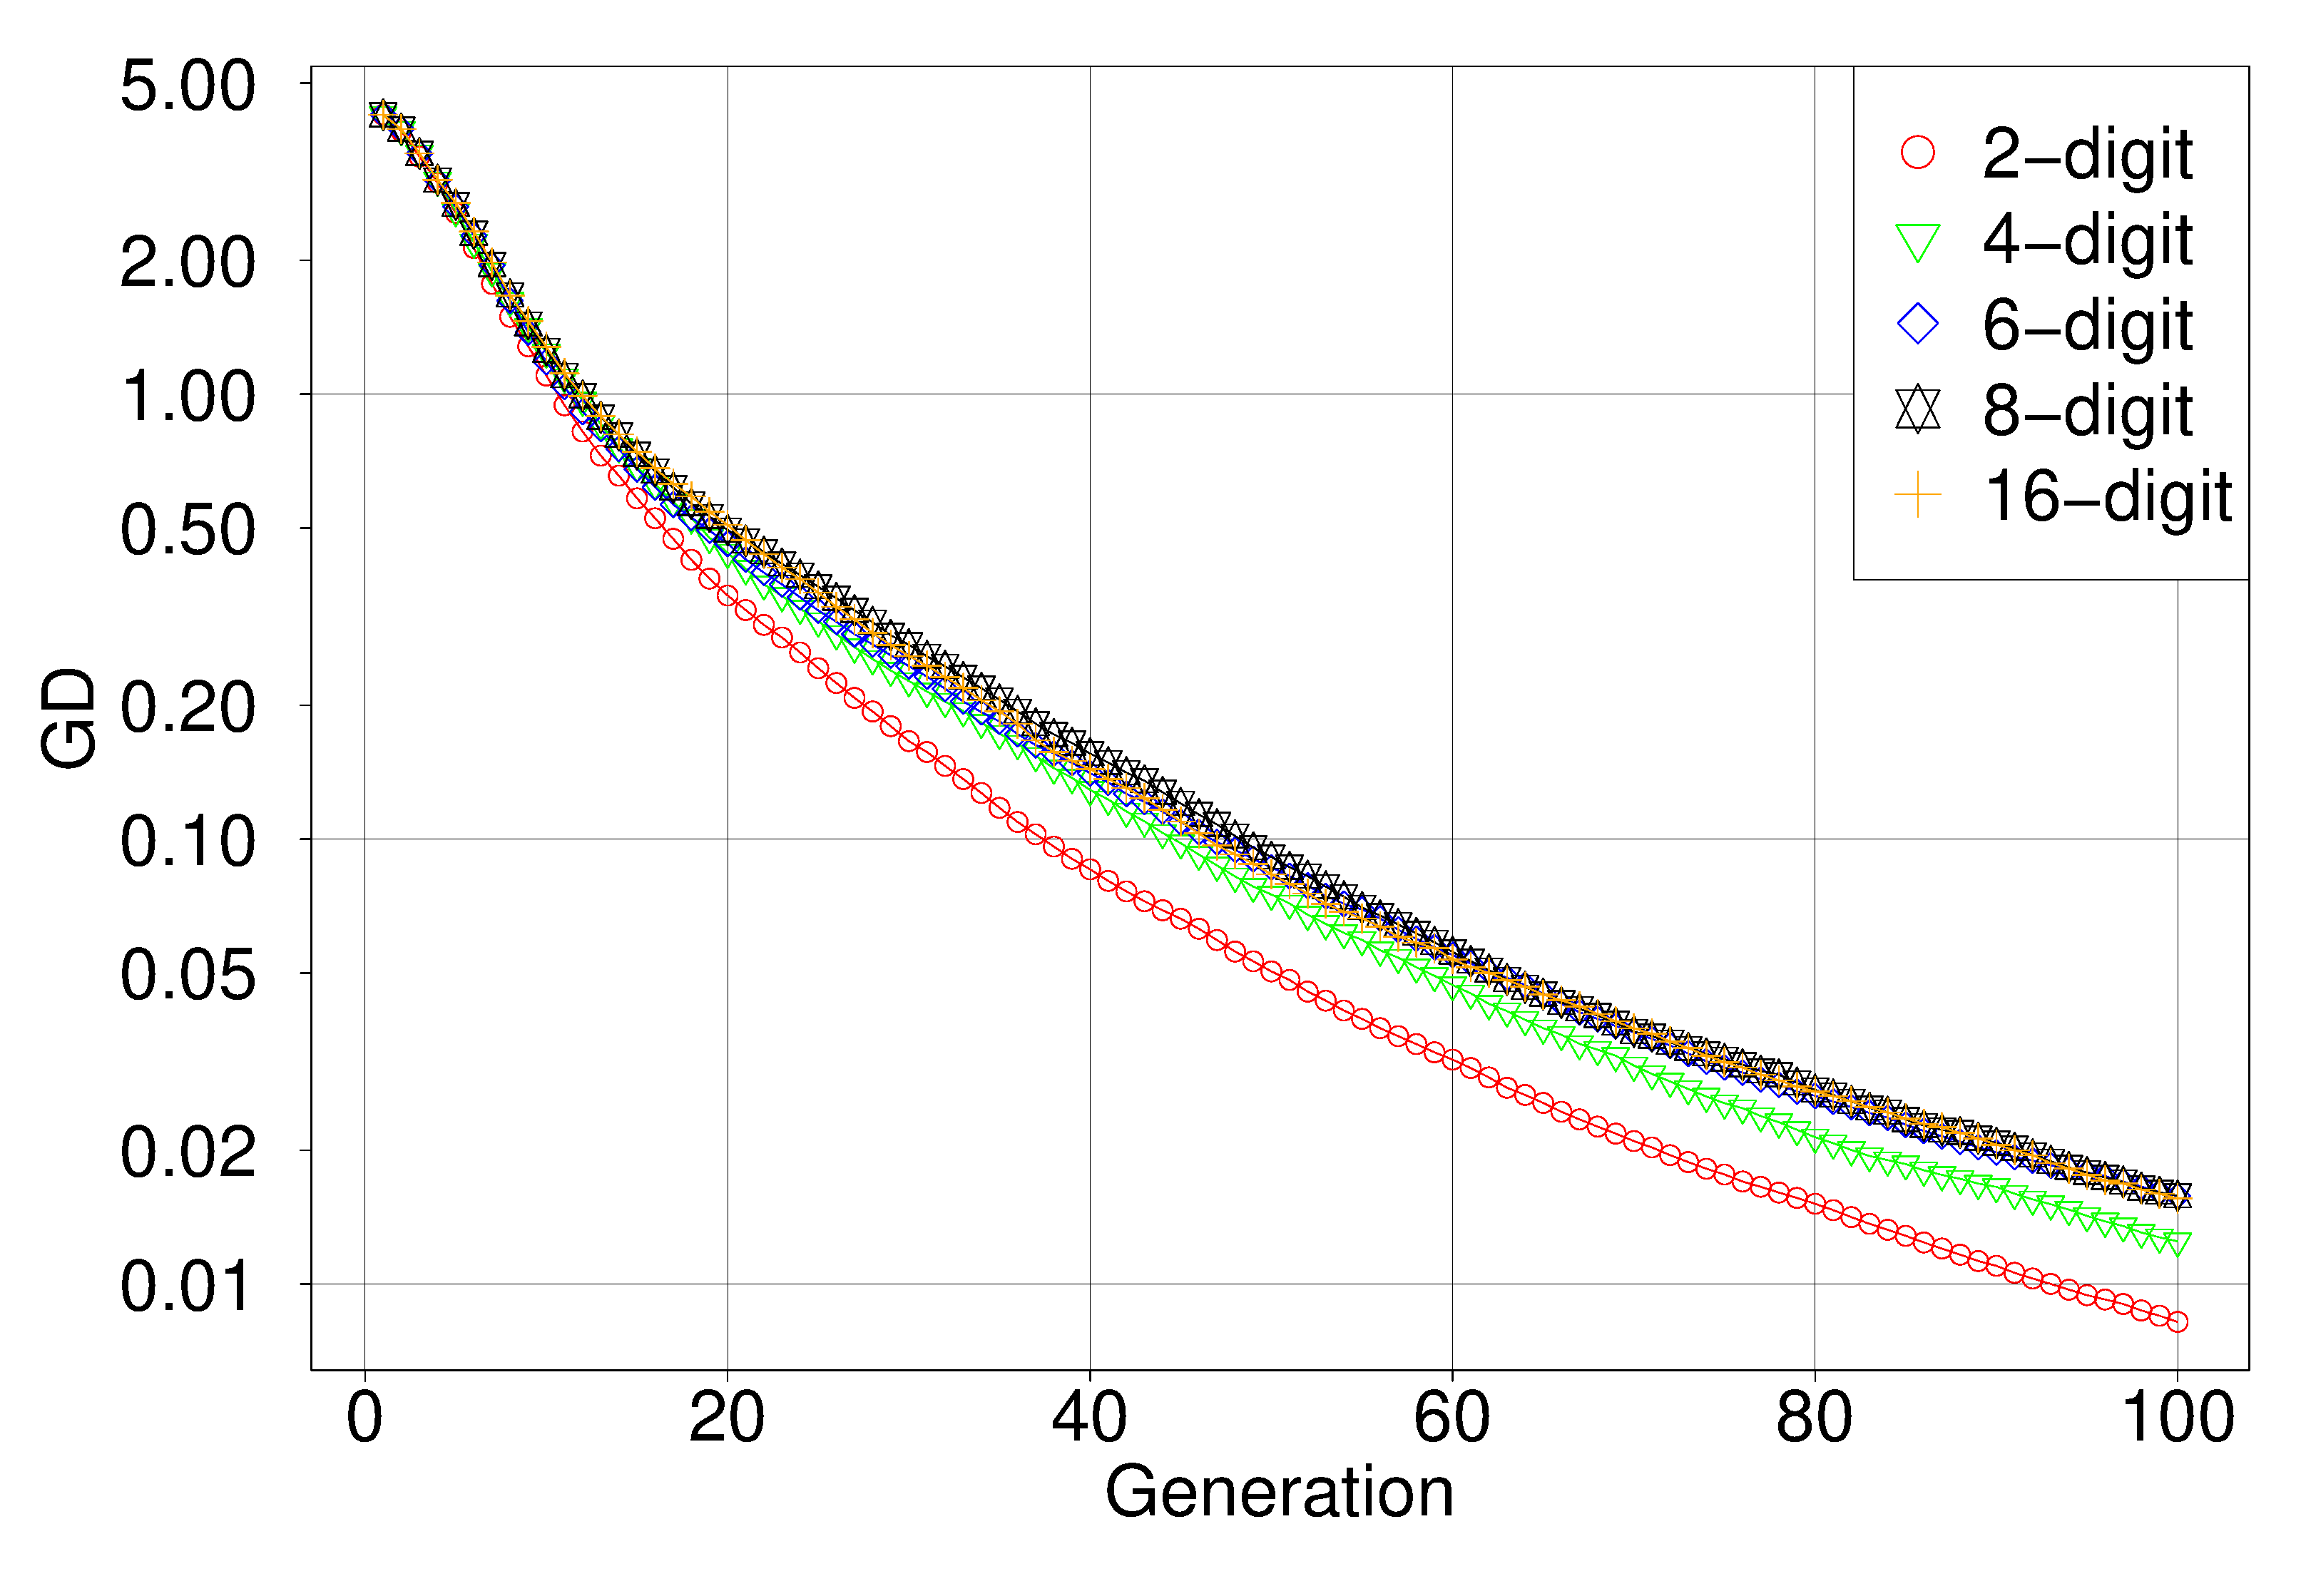
\includegraphics[width=1\linewidth]{../figures/MOEAD/DTLZ2_another_GD.eps}
\begin{center}
{\footnotesize (a) Modified DTLZ2}
\end{center}
\end{minipage}
\begin{minipage}{0.32\hsize}
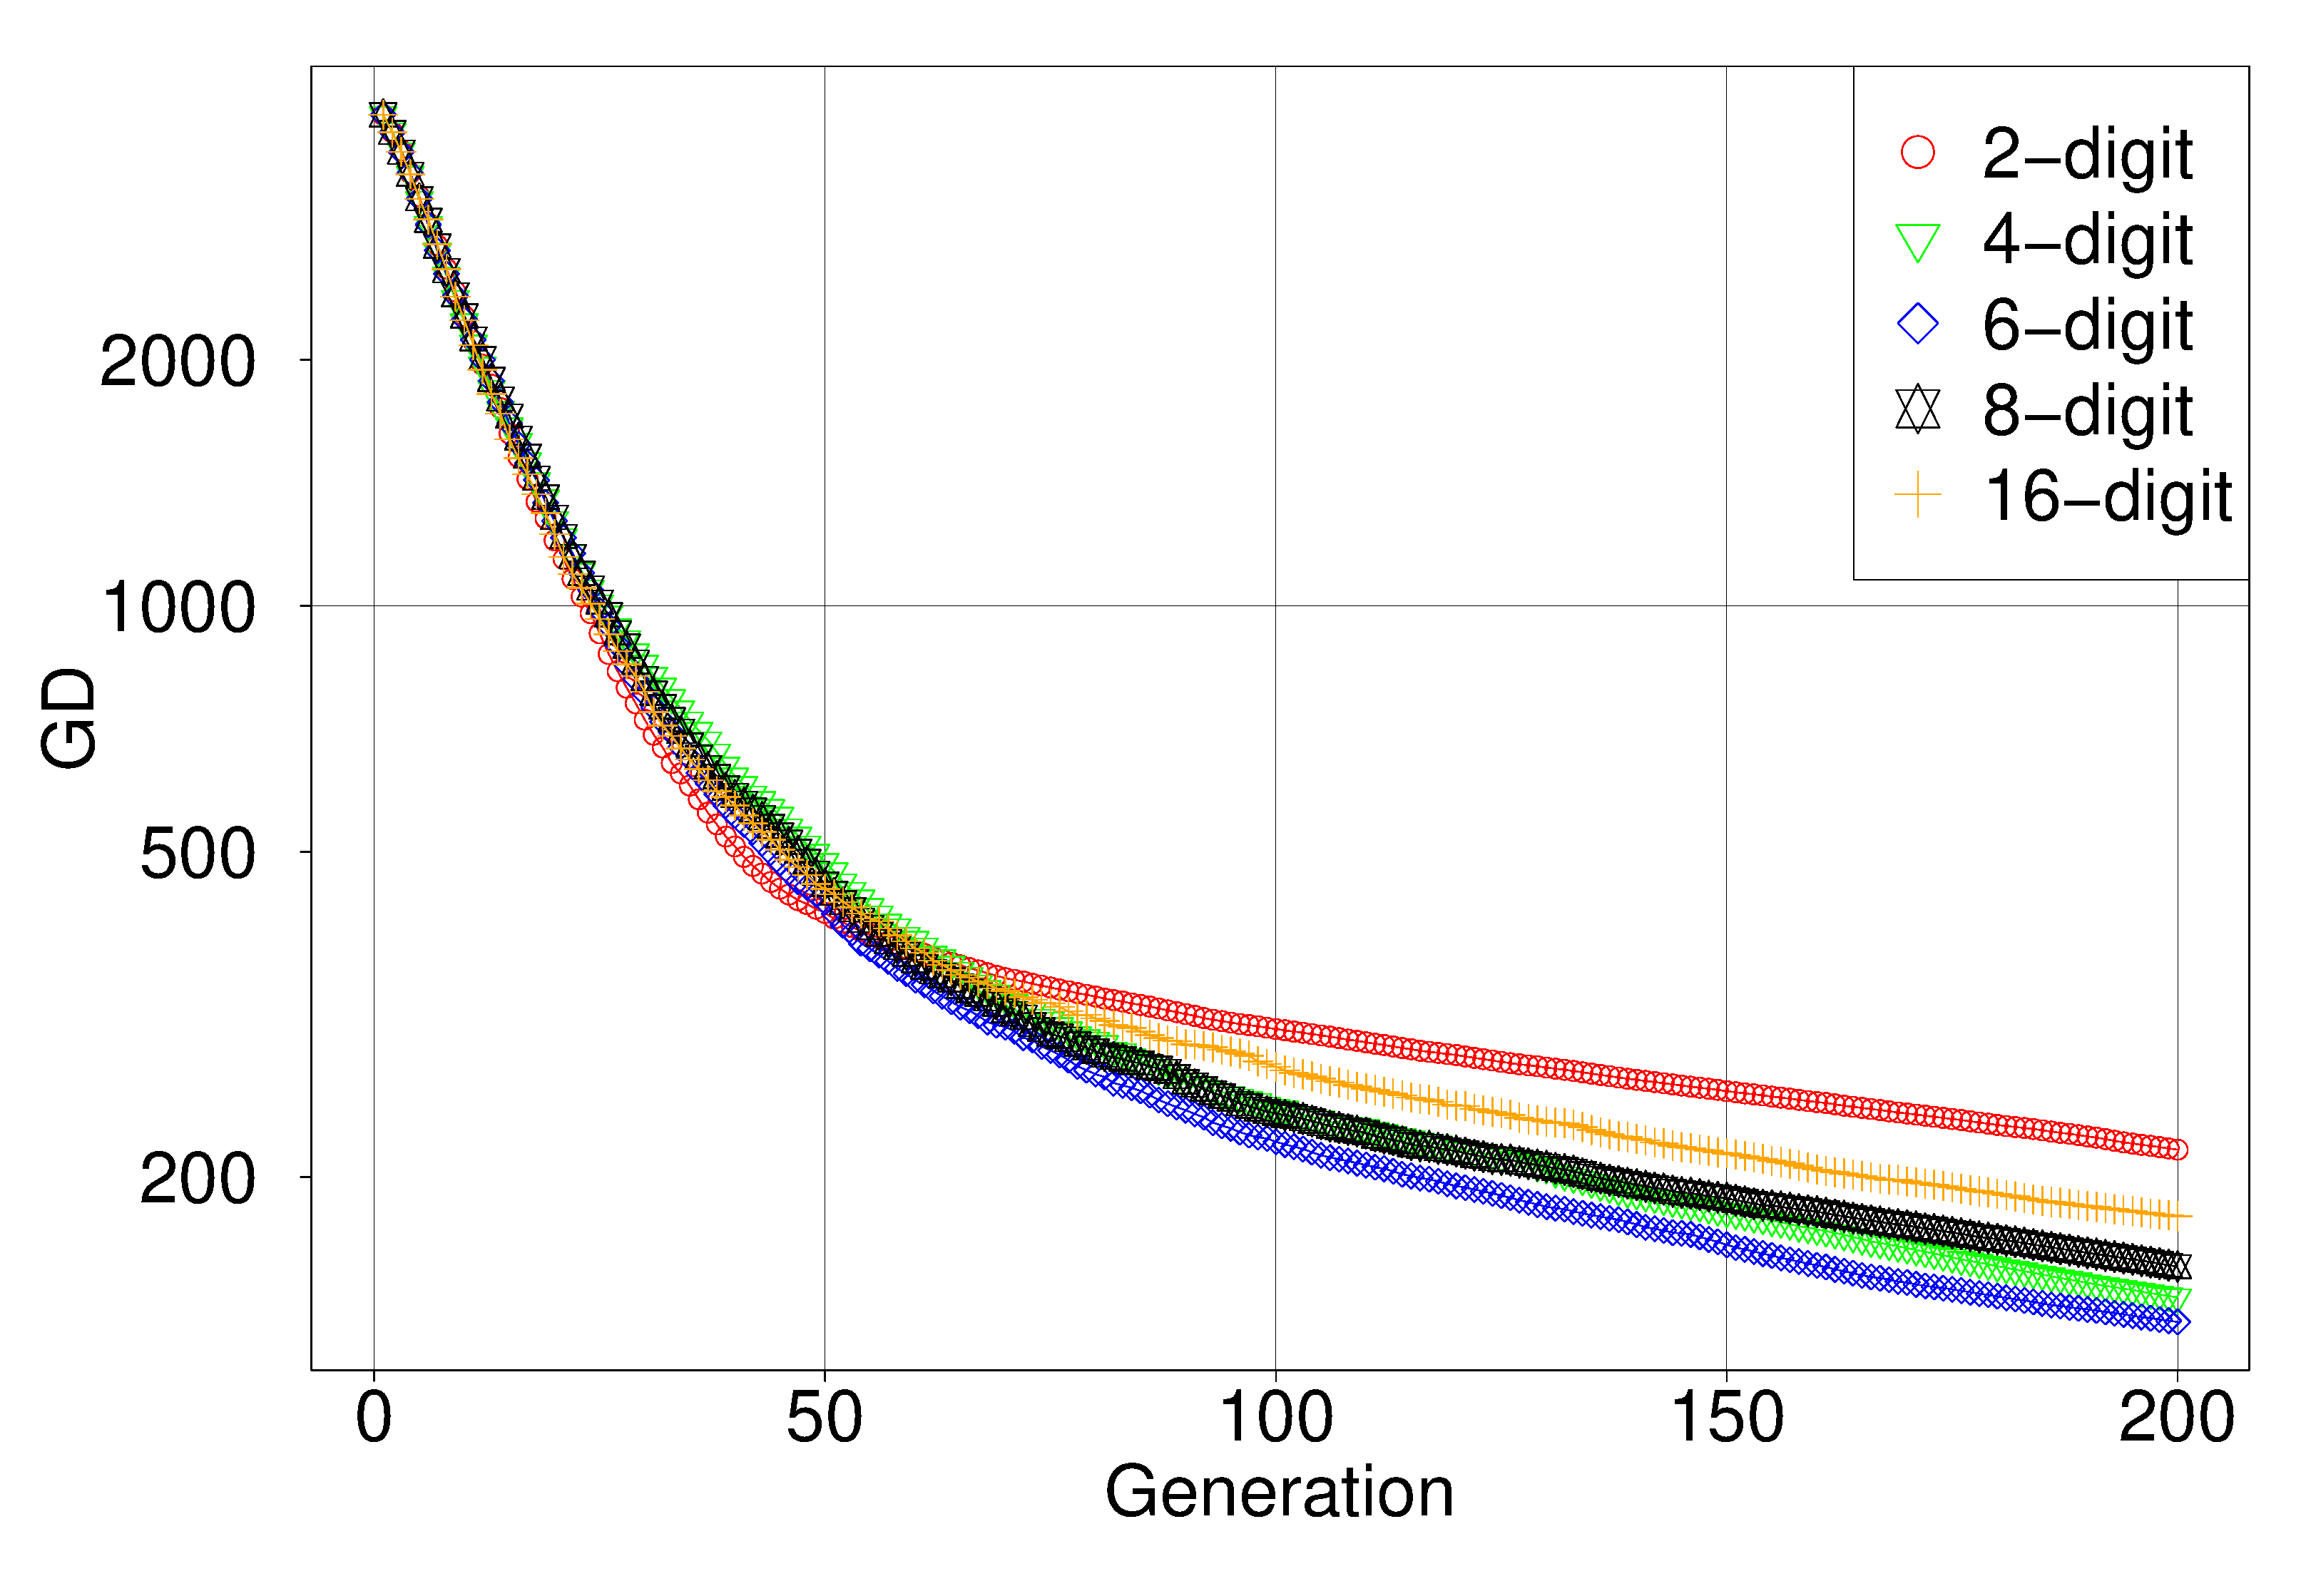
\includegraphics[width=1\linewidth]{../figures/MOEAD/DTLZ3_another_GD.eps}
\begin{center}
{\footnotesize (b) Modified DTLZ3}
\end{center}
\end{minipage}
\begin{minipage}{0.32\hsize}
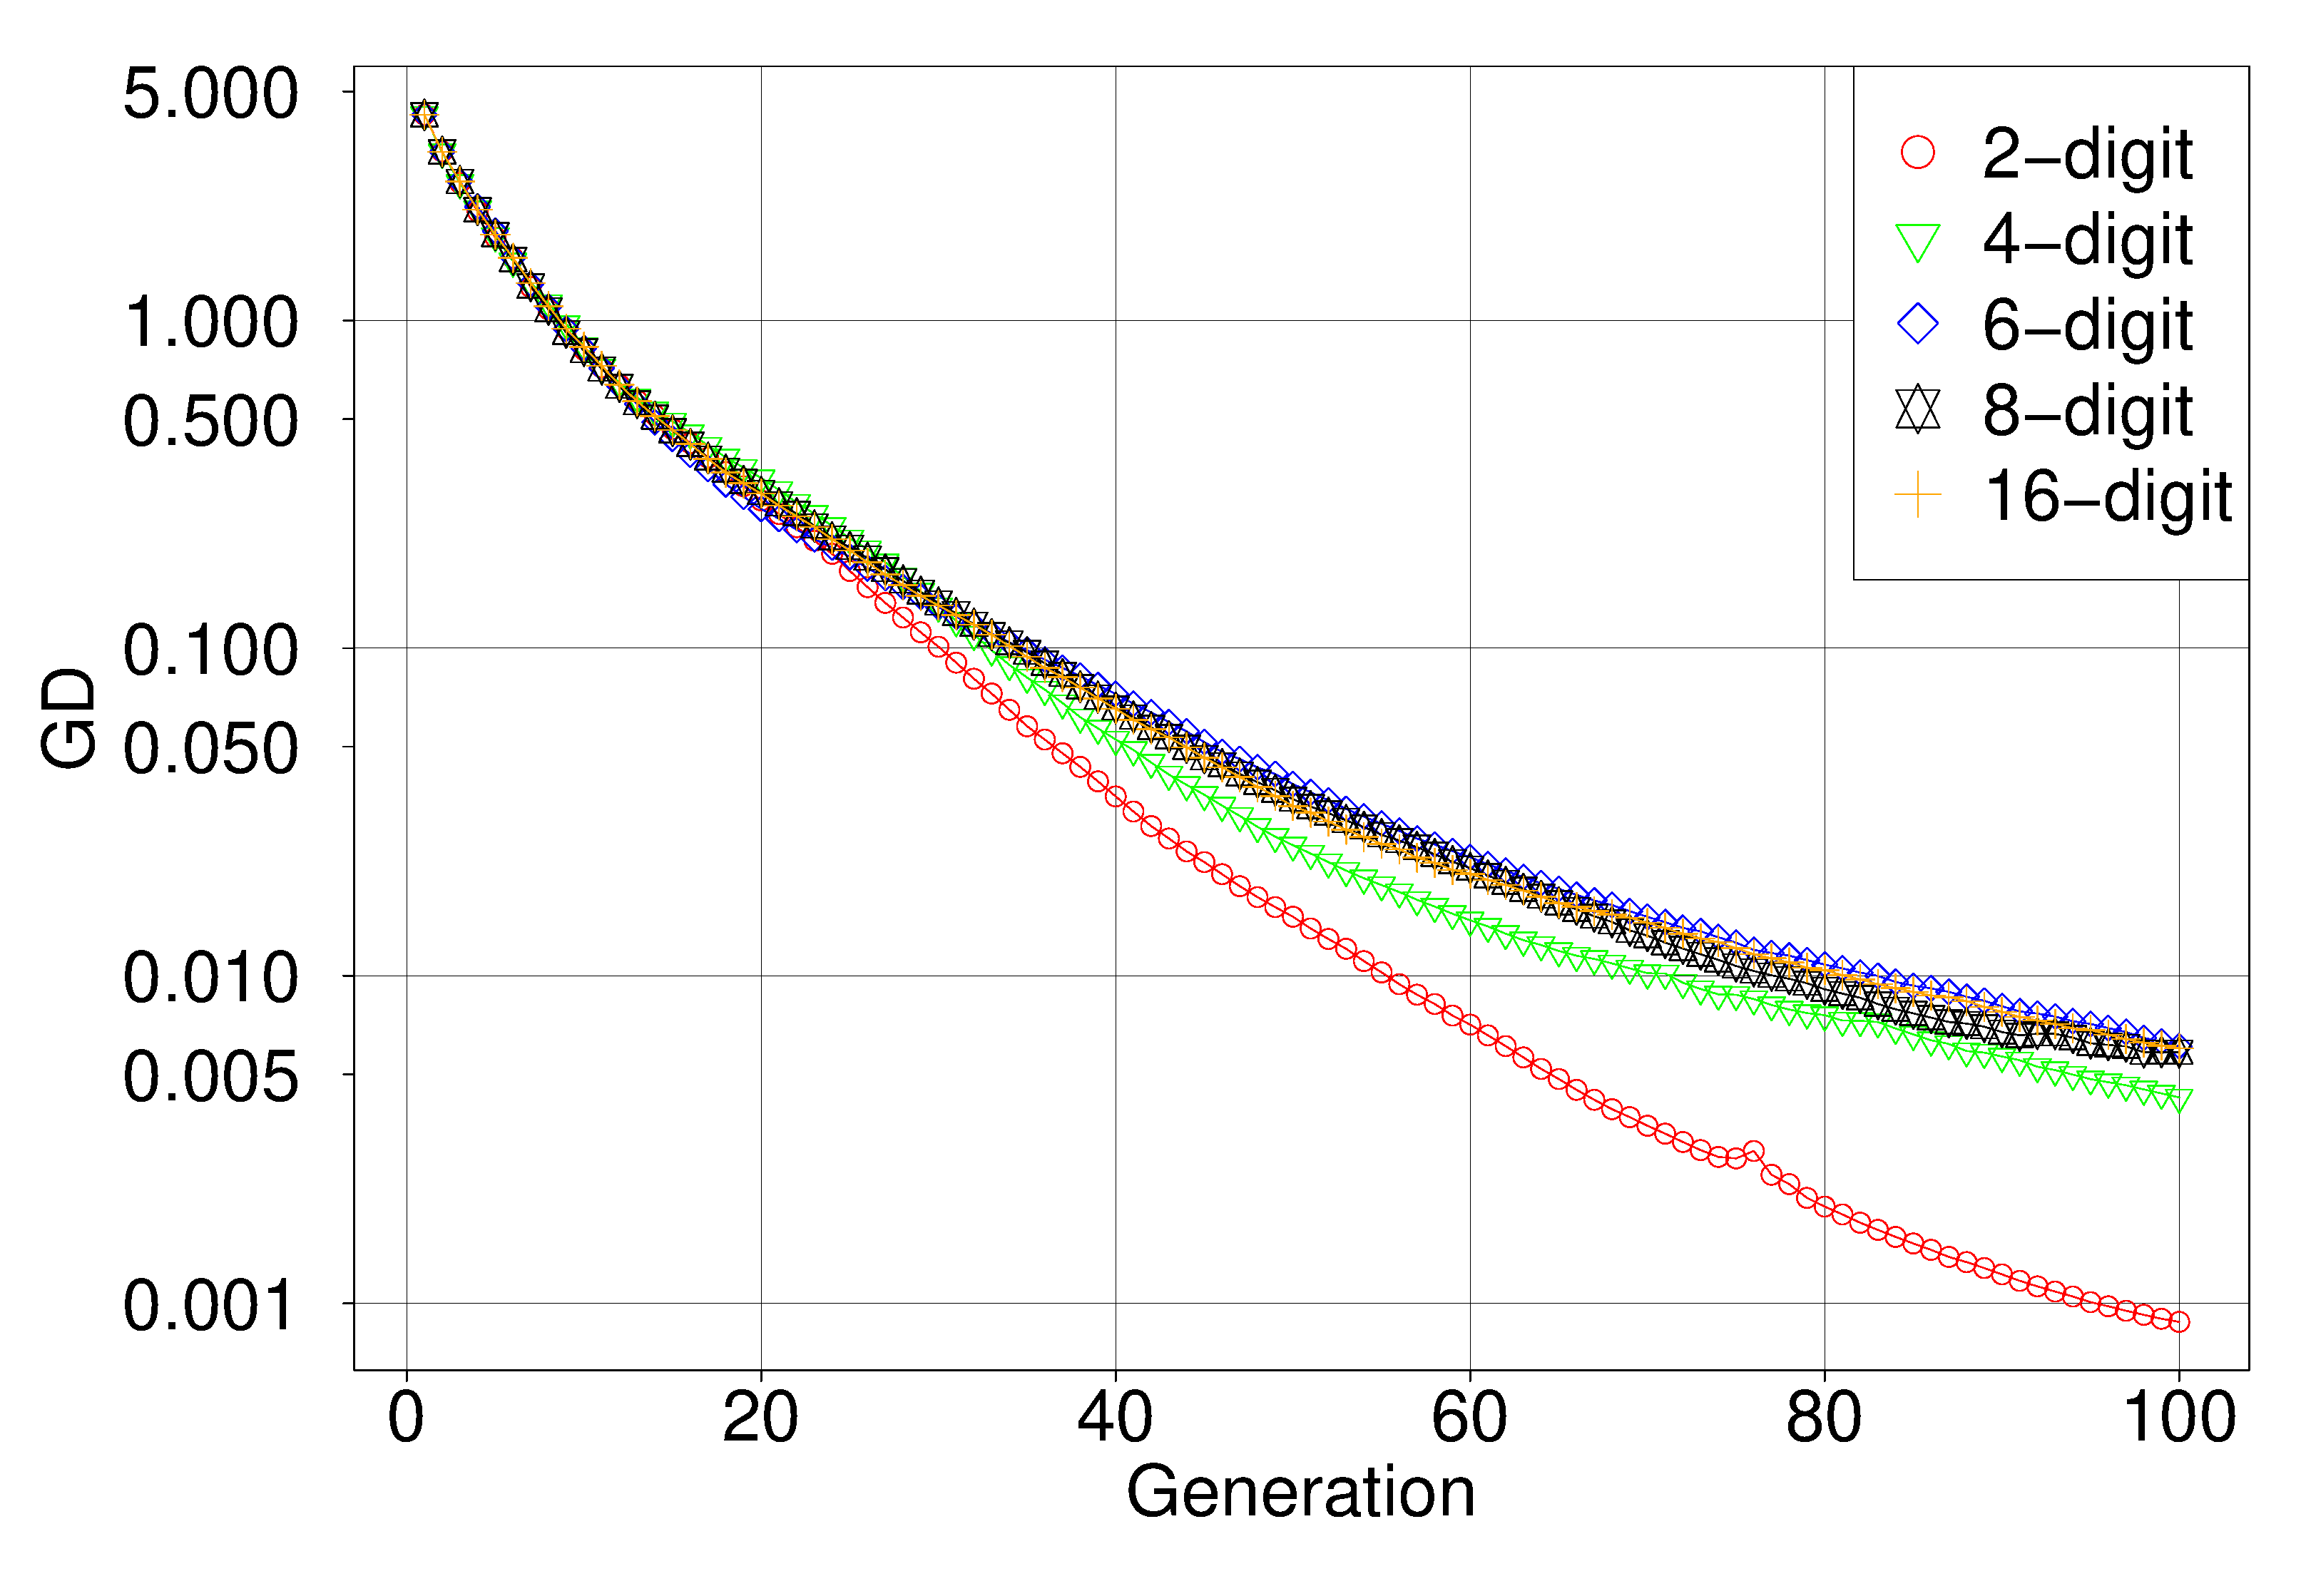
\includegraphics[width=1\linewidth]{../figures/MOEAD/DTLZ4_another_GD.eps}
\begin{center}
{\footnotesize (c) Modified DTLZ4}
\end{center}
\end{minipage}
\end{tabular}
\caption{Modified DTLZ2-4におけるGDの推移(MOEA/D)}
\label{fig:gd_mod_moead}
\end{figure*}

\begin{figure*}[htbp]
\begin{tabular}{cc}
\begin{minipage}{0.32\hsize}
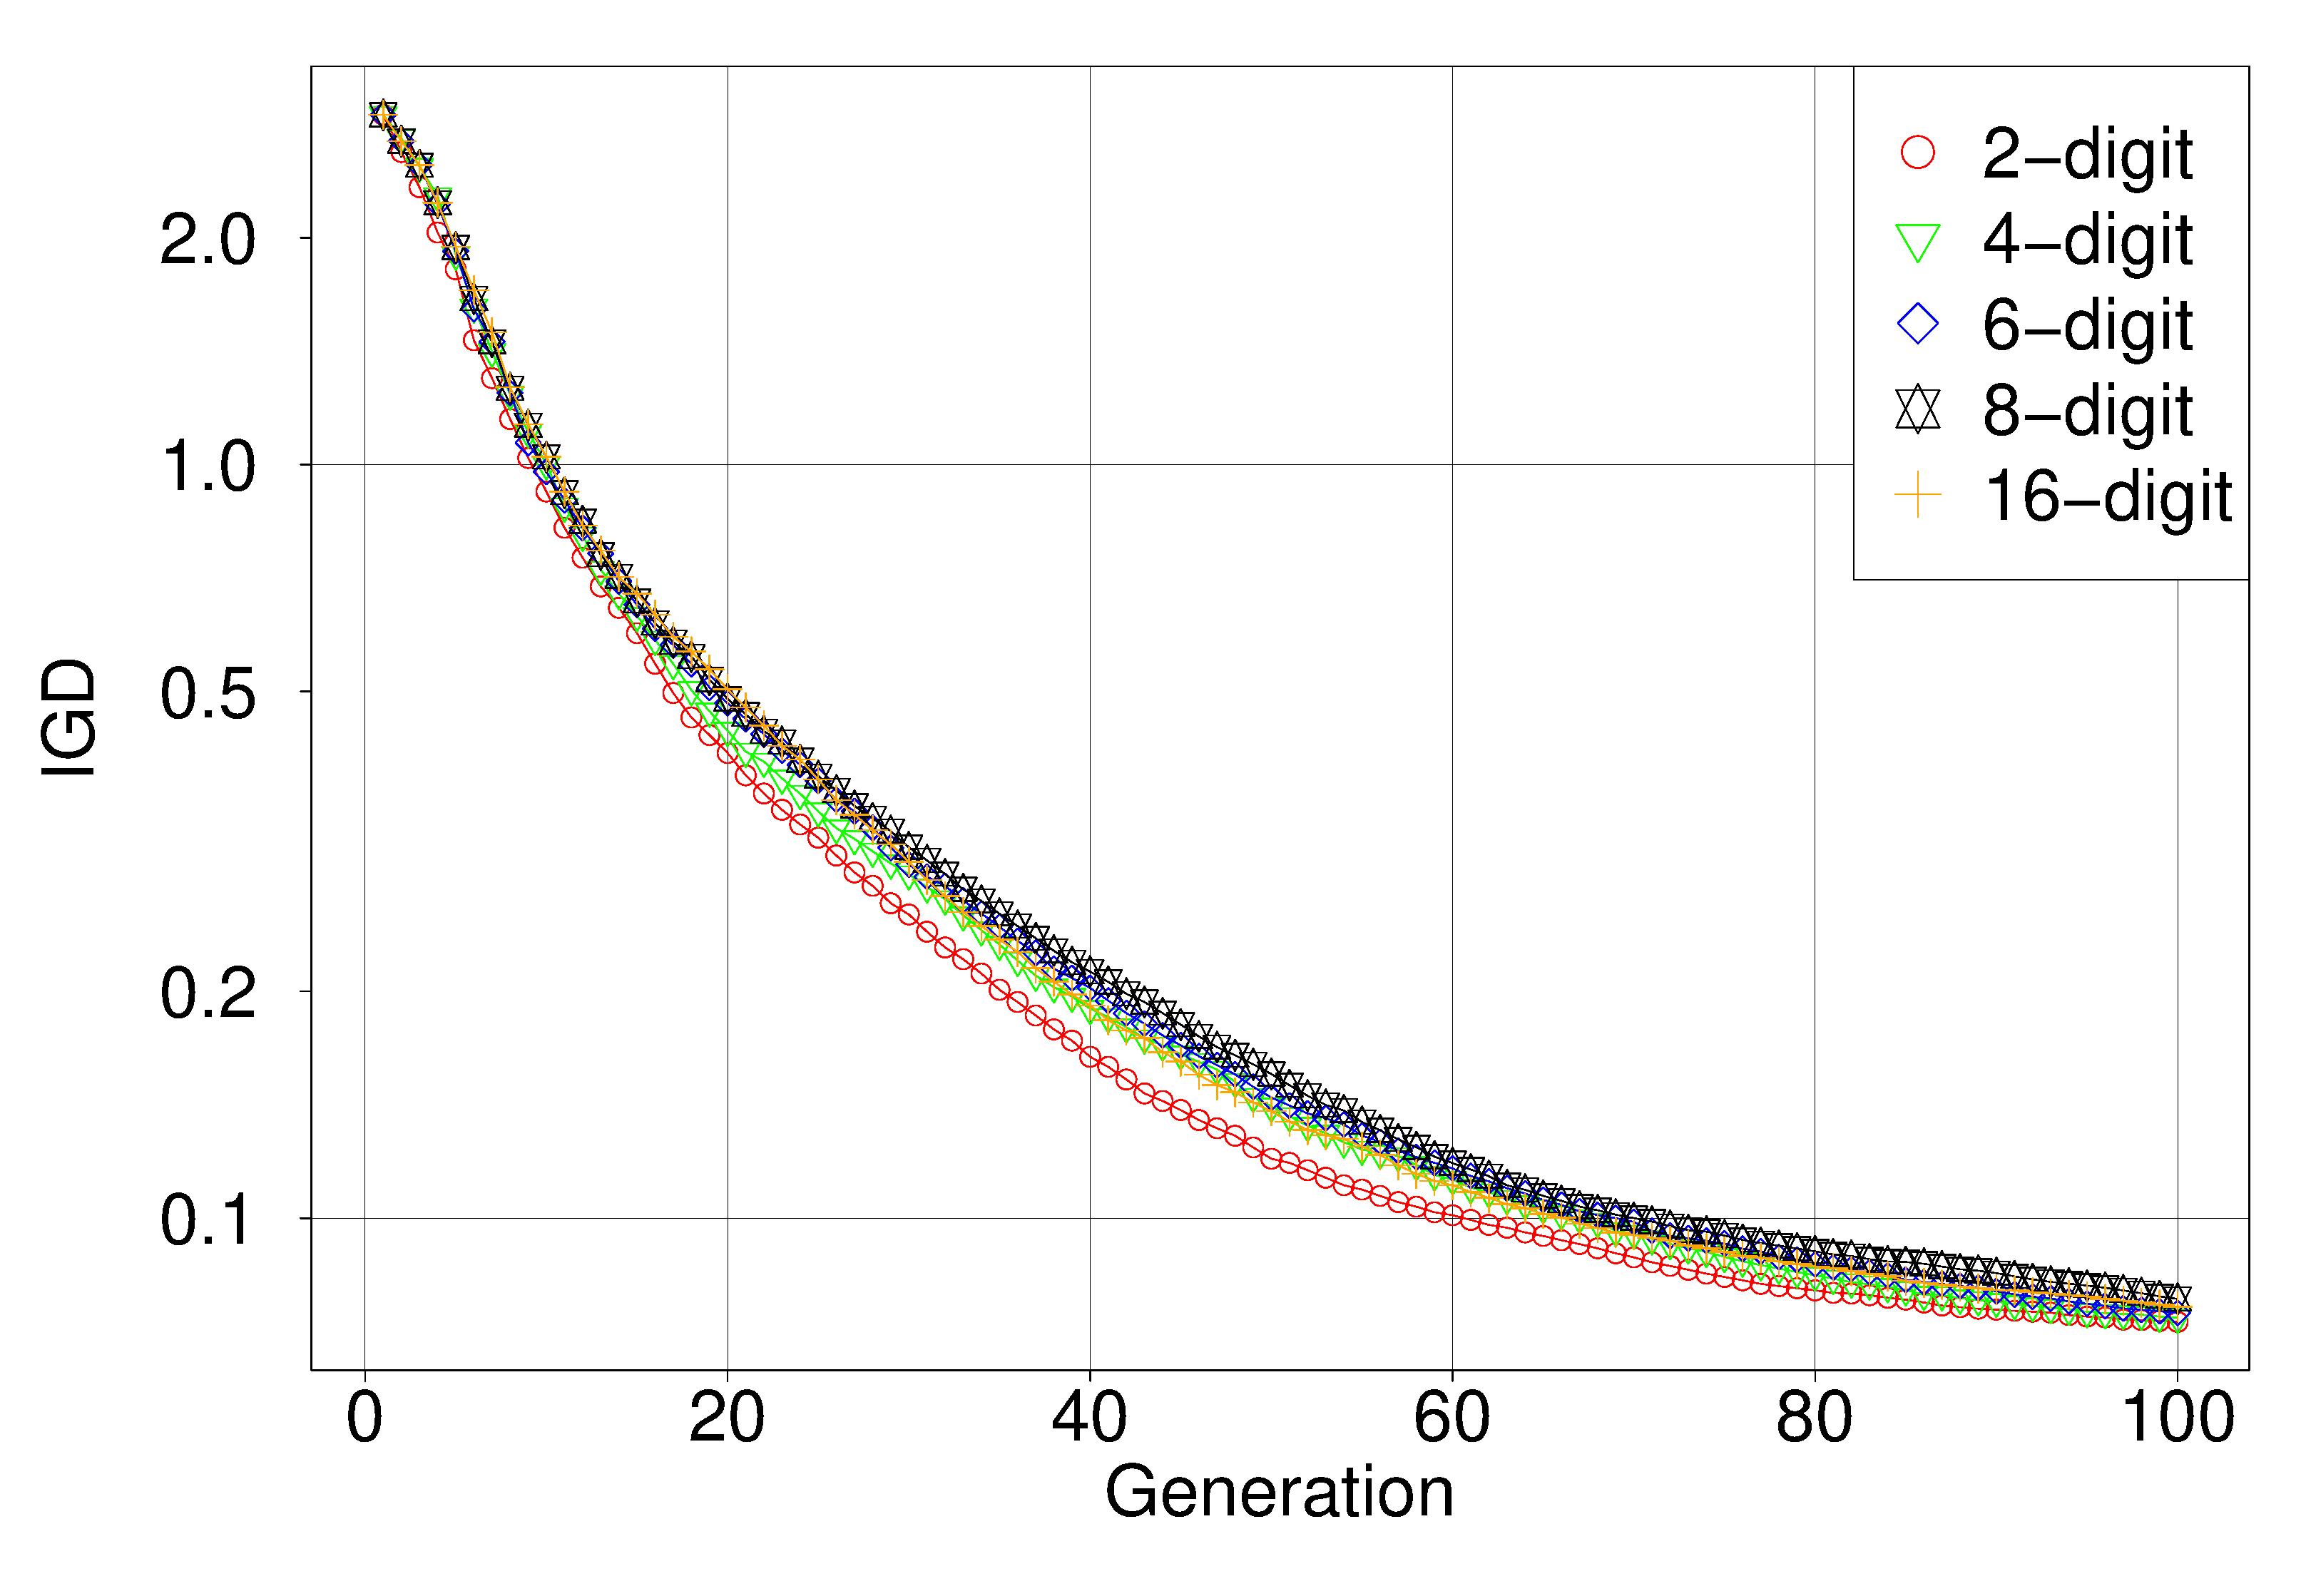
\includegraphics[width=1\linewidth]{../figures/MOEAD/DTLZ2_another_IGD.eps}
\begin{center}
{\footnotesize (a) Modified DTLZ2}
\end{center}
\end{minipage}
\begin{minipage}{0.32\hsize}
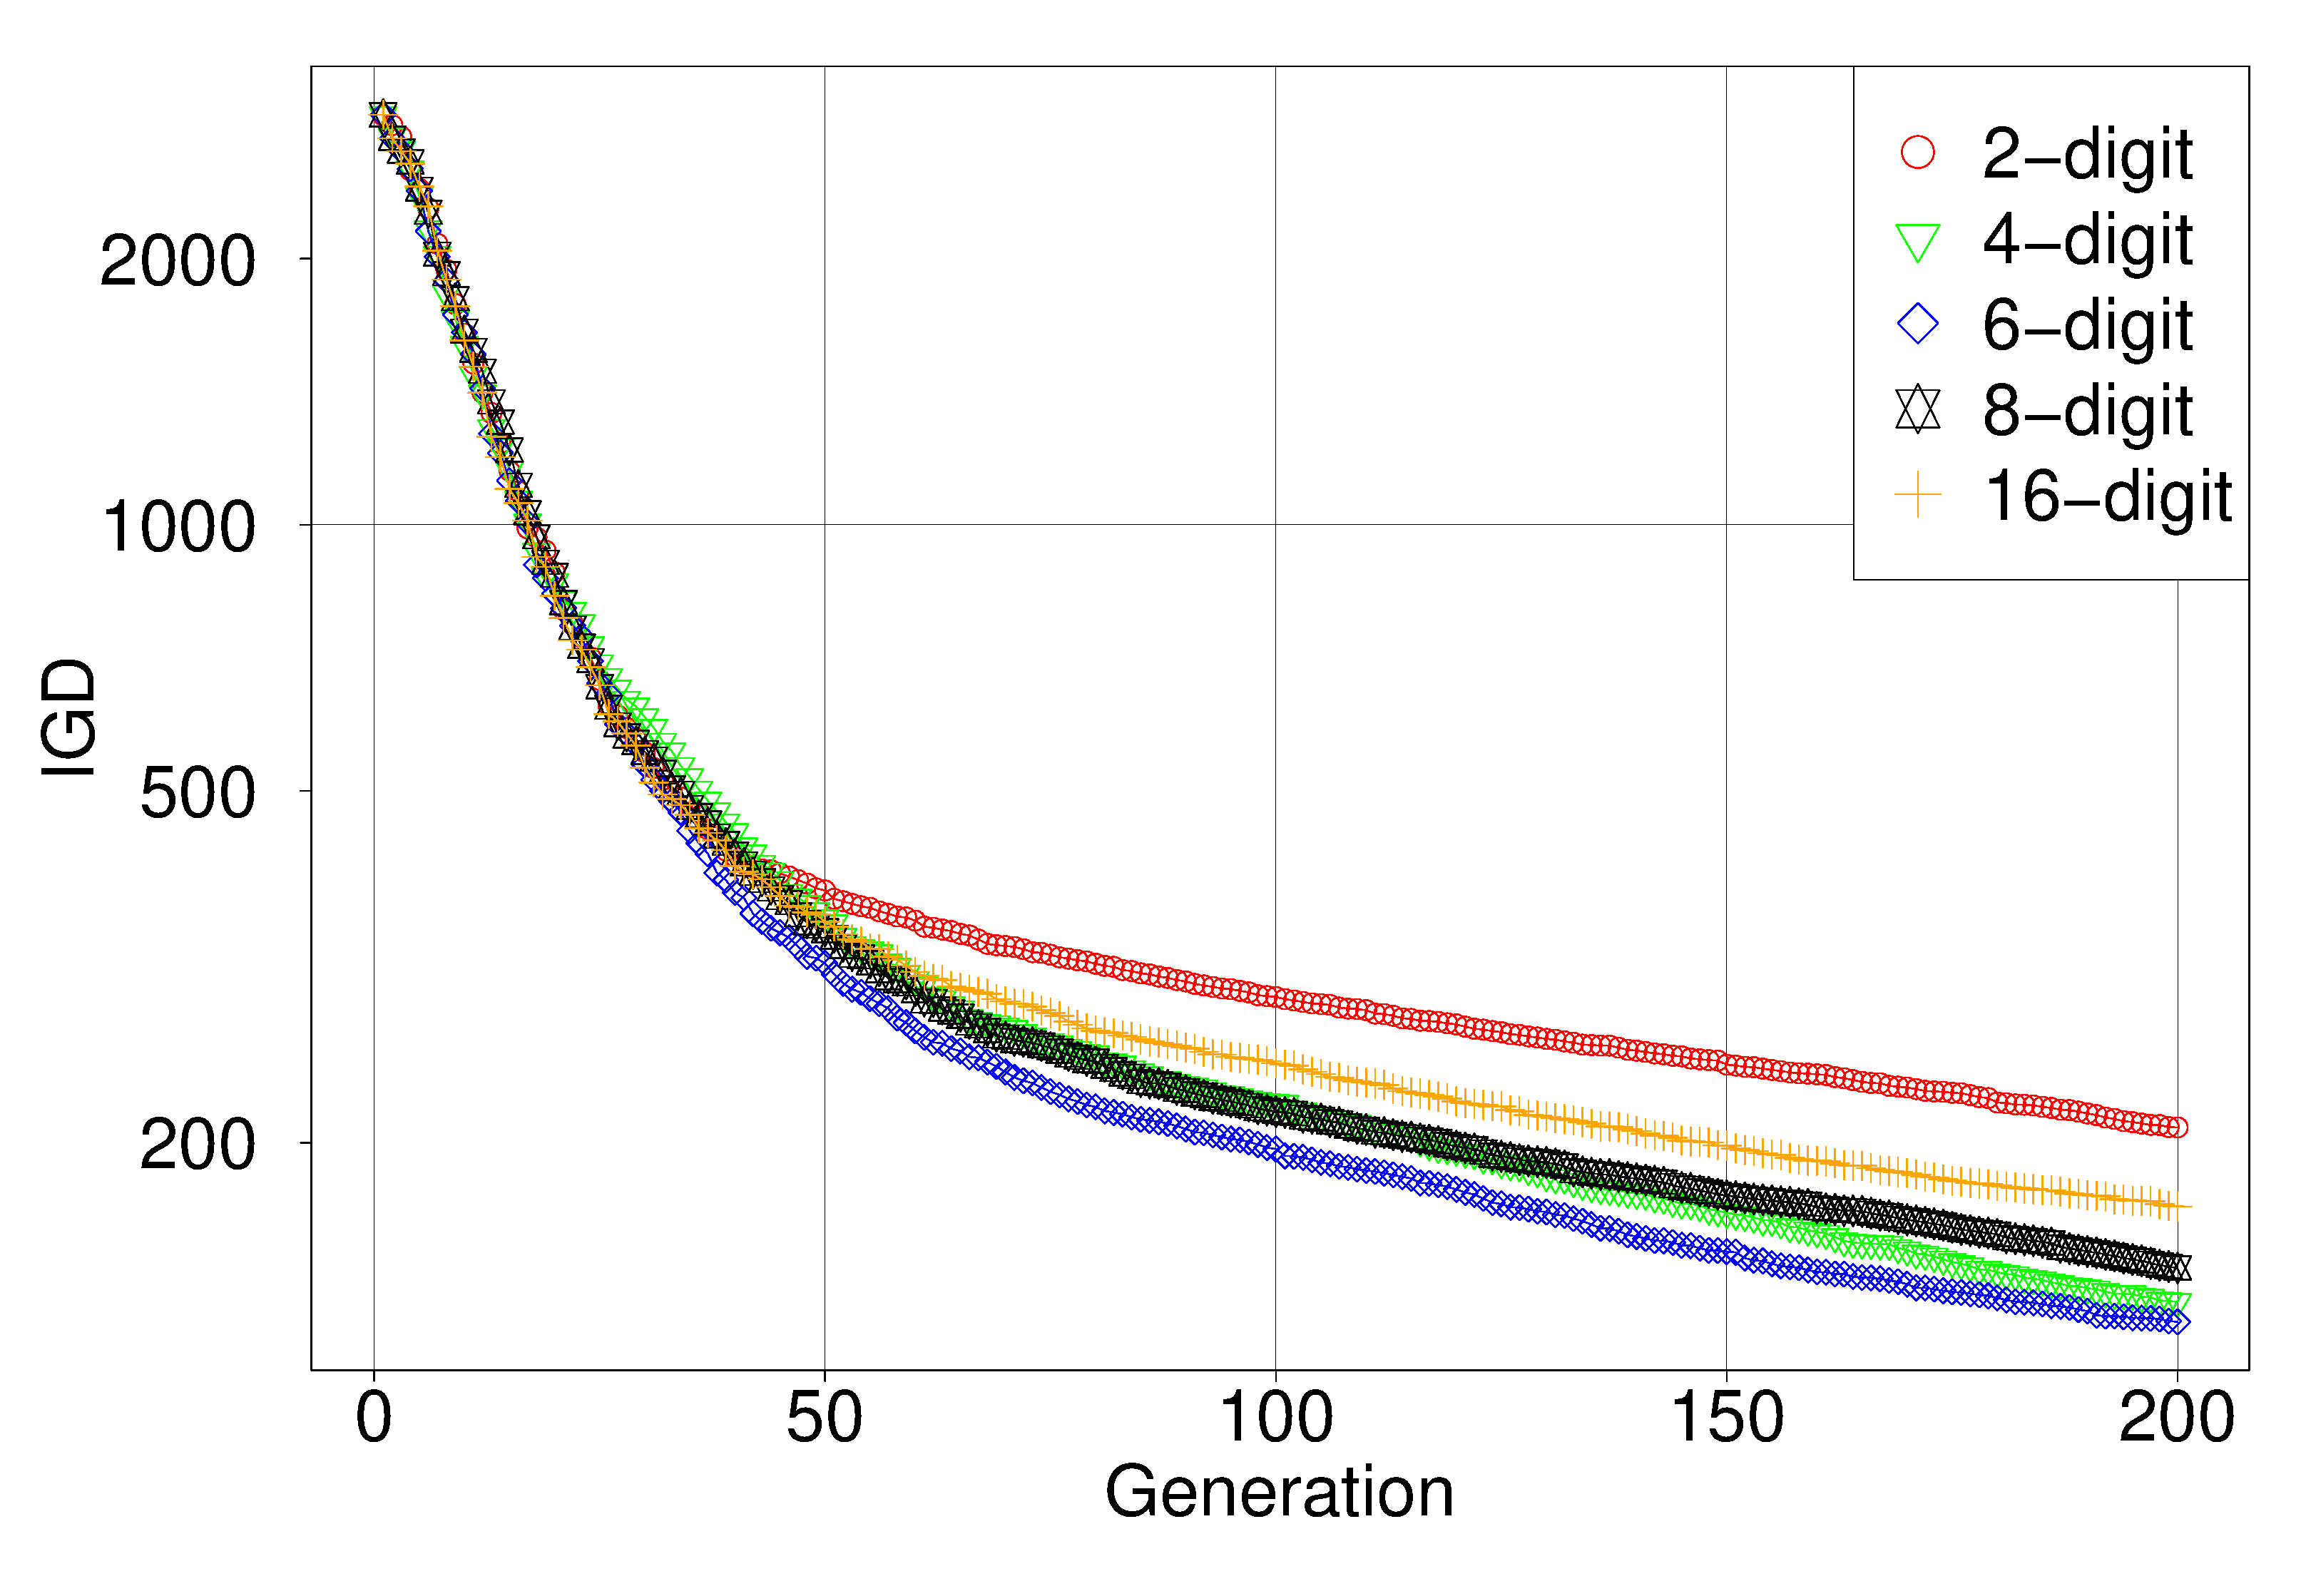
\includegraphics[width=1\linewidth]{../figures/MOEAD/DTLZ3_another_IGD.eps}
\begin{center}
{\footnotesize (b) Modified DTLZ3}
\end{center}
\end{minipage}
\begin{minipage}{0.32\hsize}
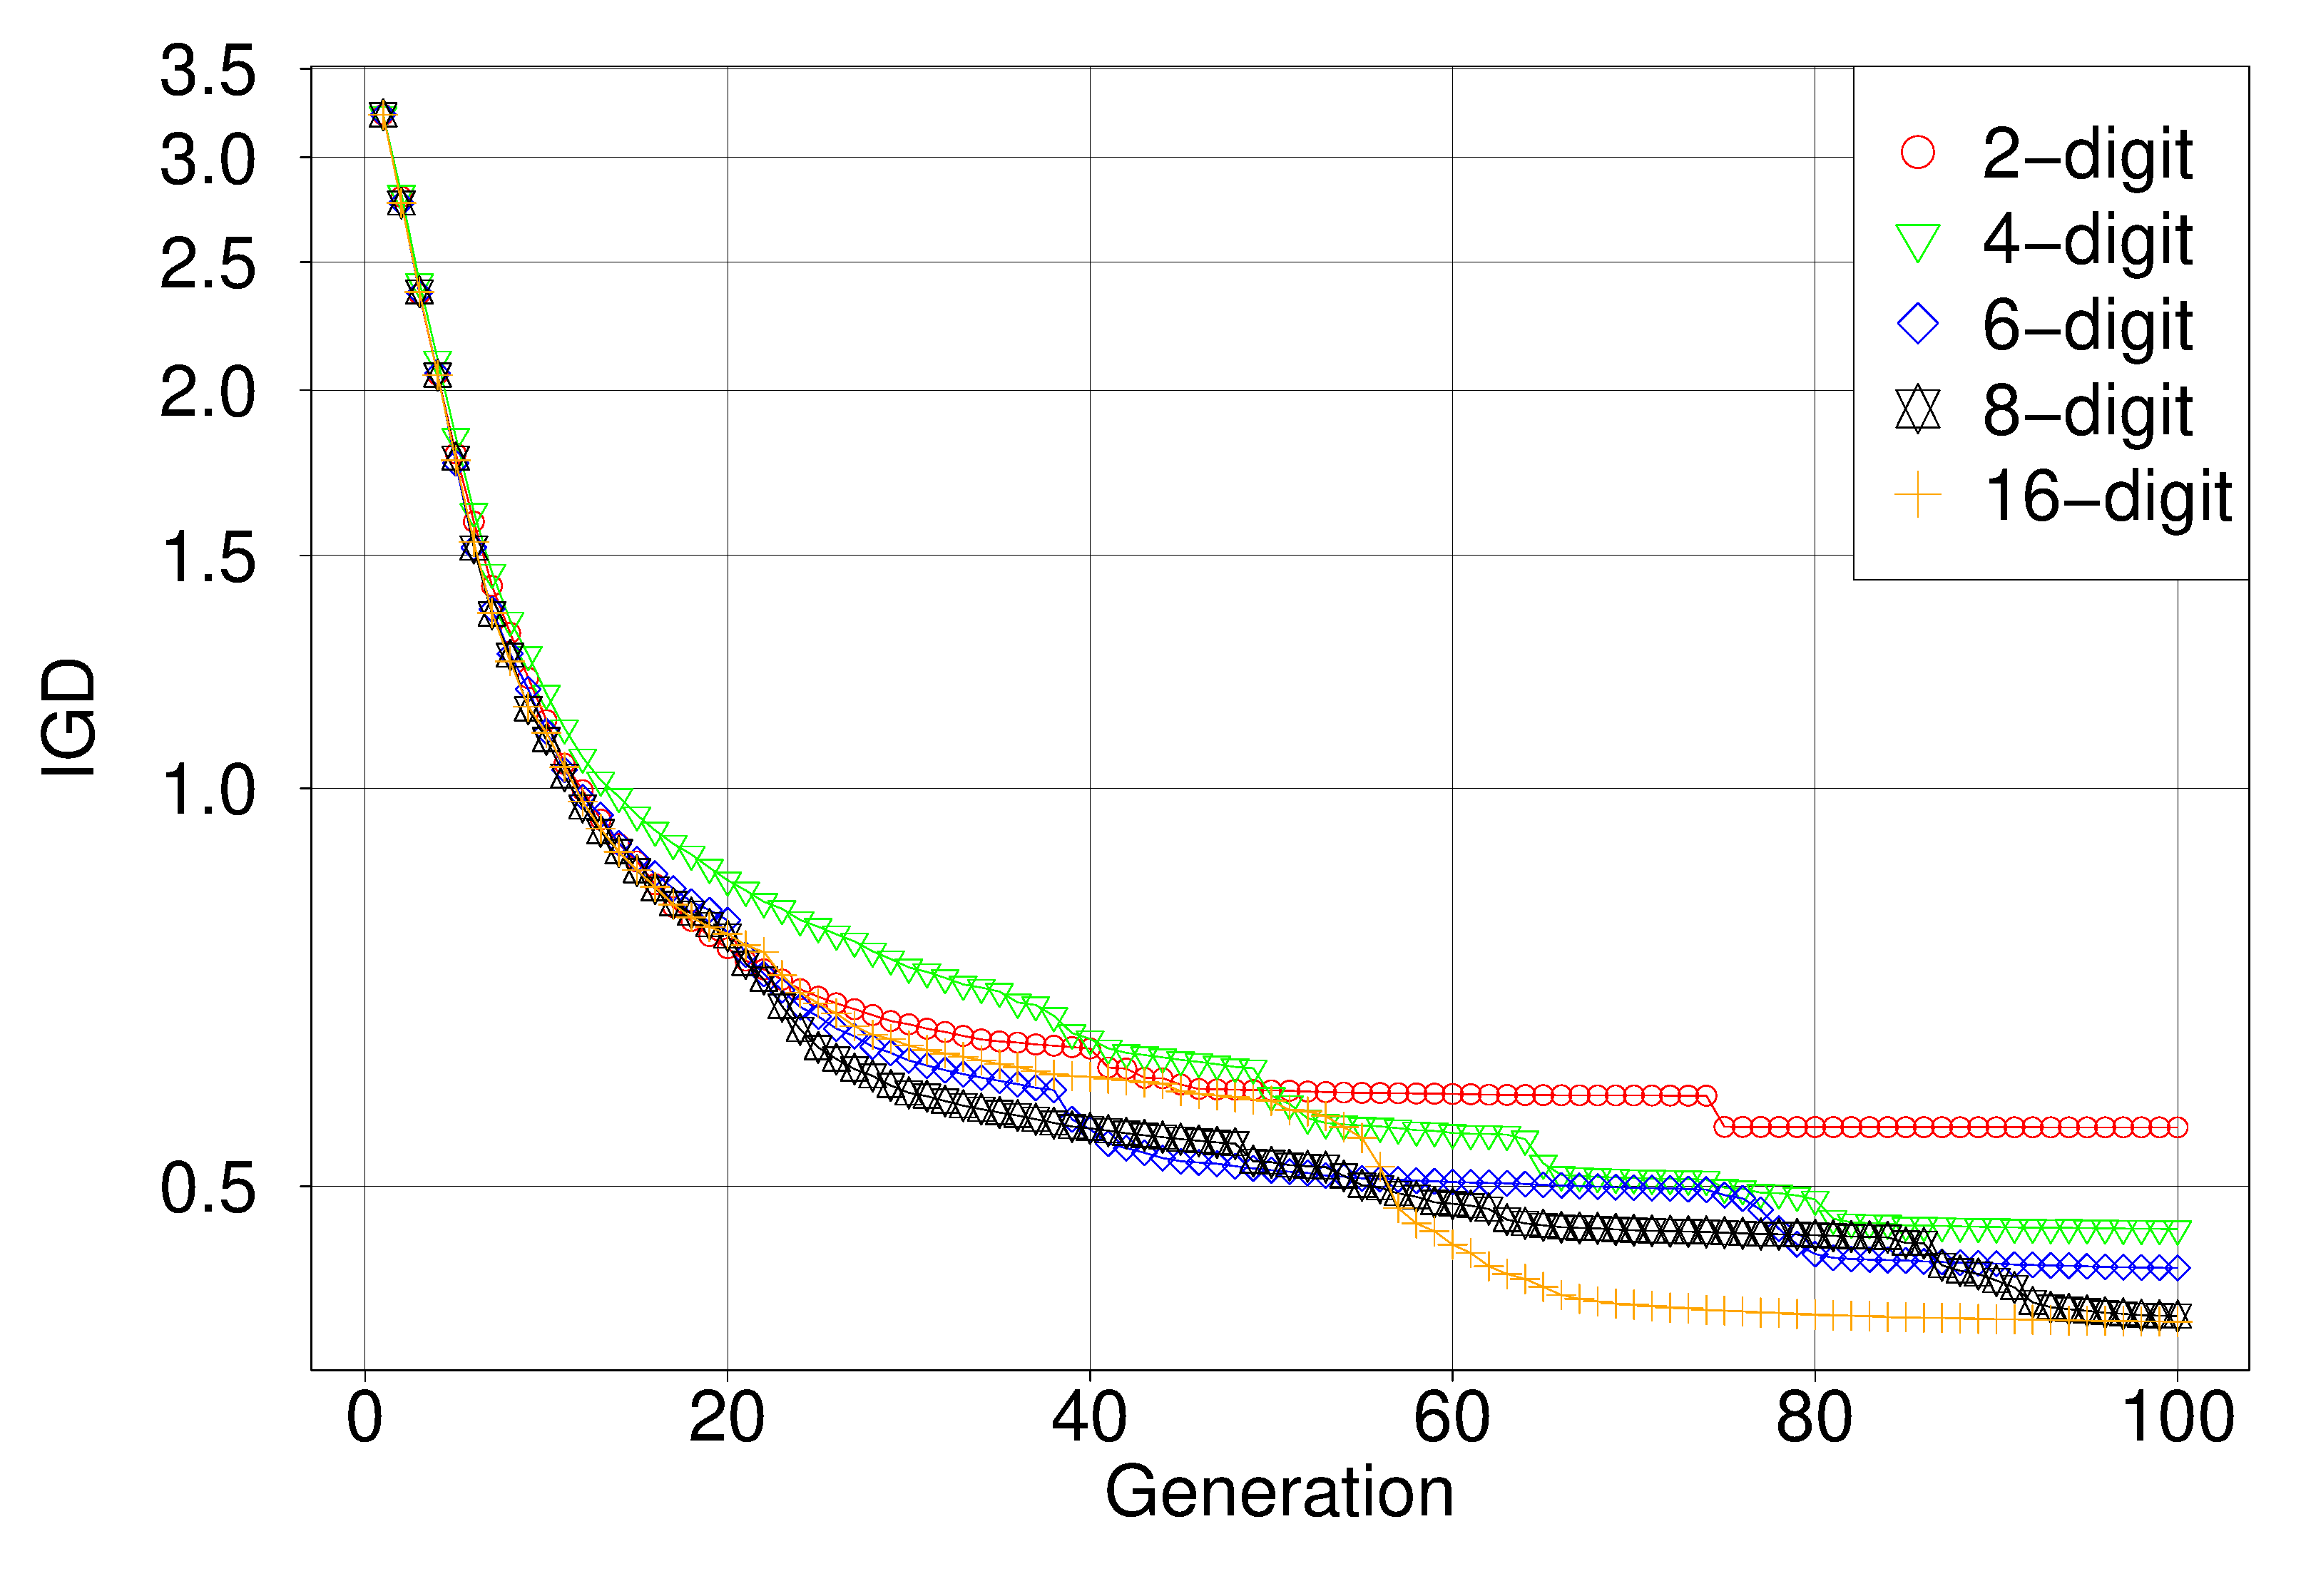
\includegraphics[width=1\linewidth]{../figures/MOEAD/DTLZ4_another_IGD.eps}
\begin{center}
{\footnotesize (c) Modified DTLZ4}
\end{center}
\end{minipage}
\end{tabular}
\caption{Modified DTLZ2-4におけるIGDの推移(MOEA/D)}
\label{fig:igd_mod_moead}
\end{figure*}

\begin{figure*}[htbp]
\begin{tabular}{cc}
\begin{minipage}{0.32\hsize}
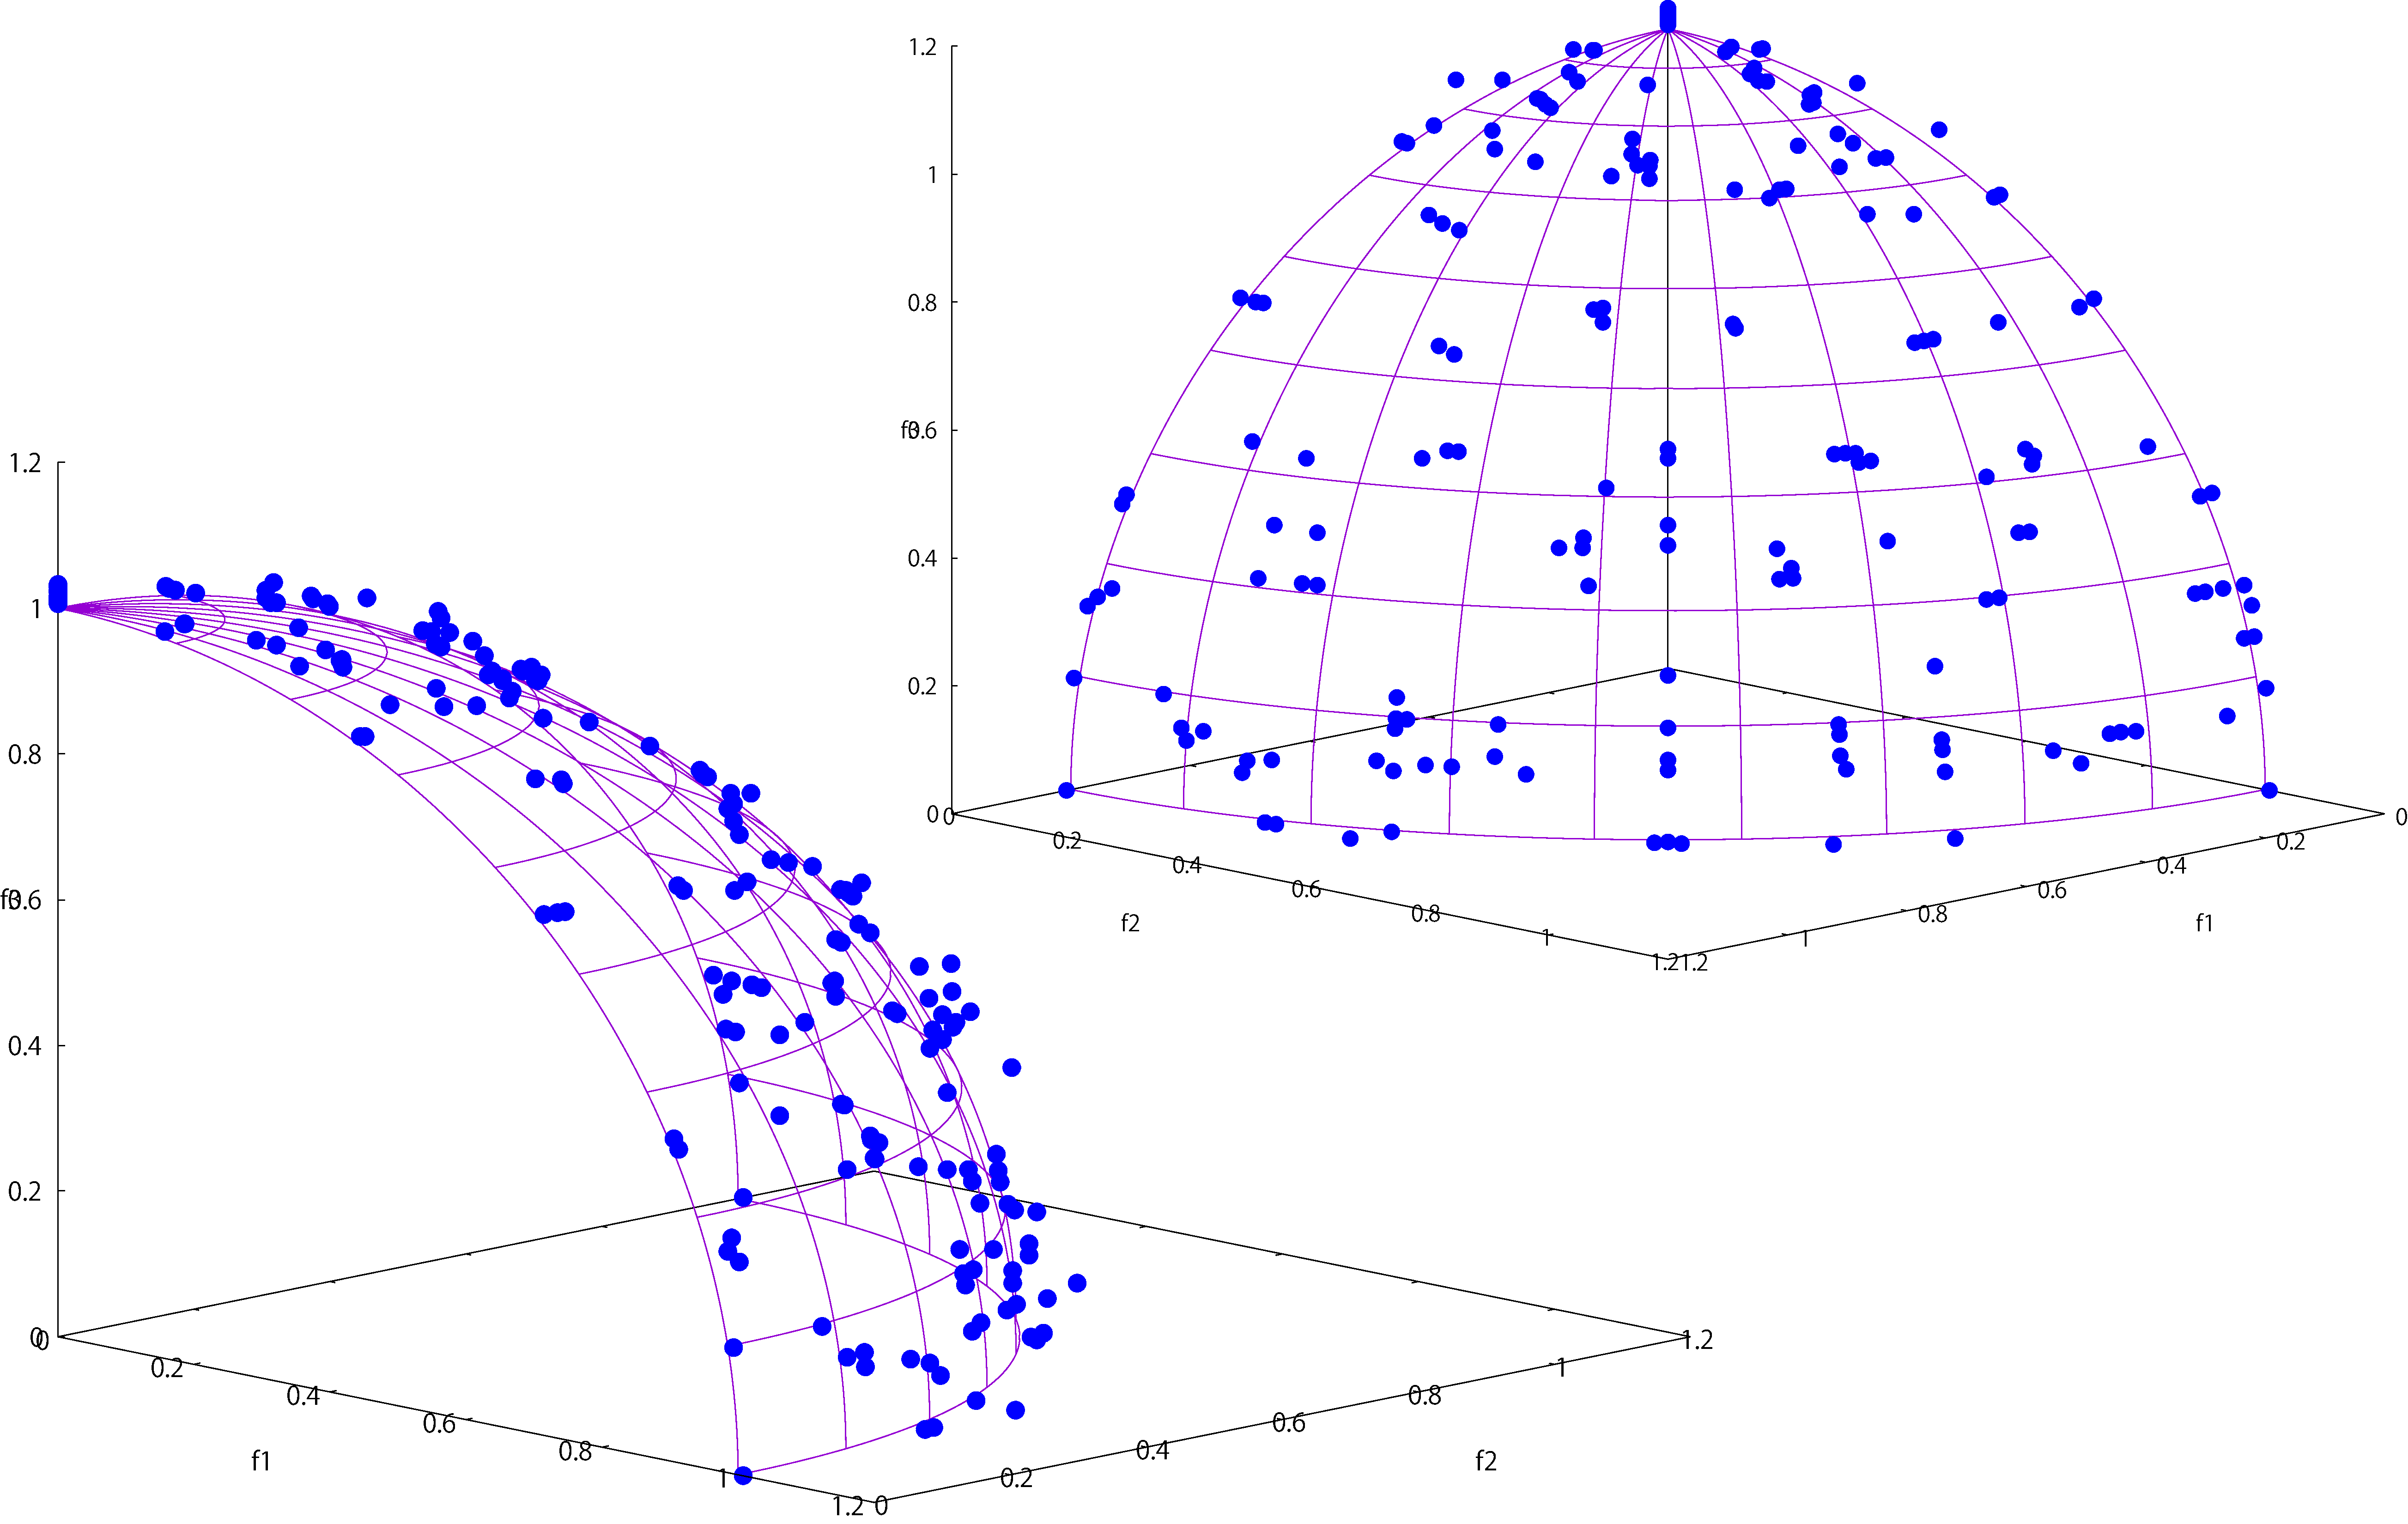
\includegraphics[width=1\linewidth]{../figures/MOEAD/DTLZ2_another_digi2_double.pdf}
\begin{center}
{\footnotesize (a) 2-digit resolution}
\end{center}
\end{minipage}
\begin{minipage}{0.32\hsize}
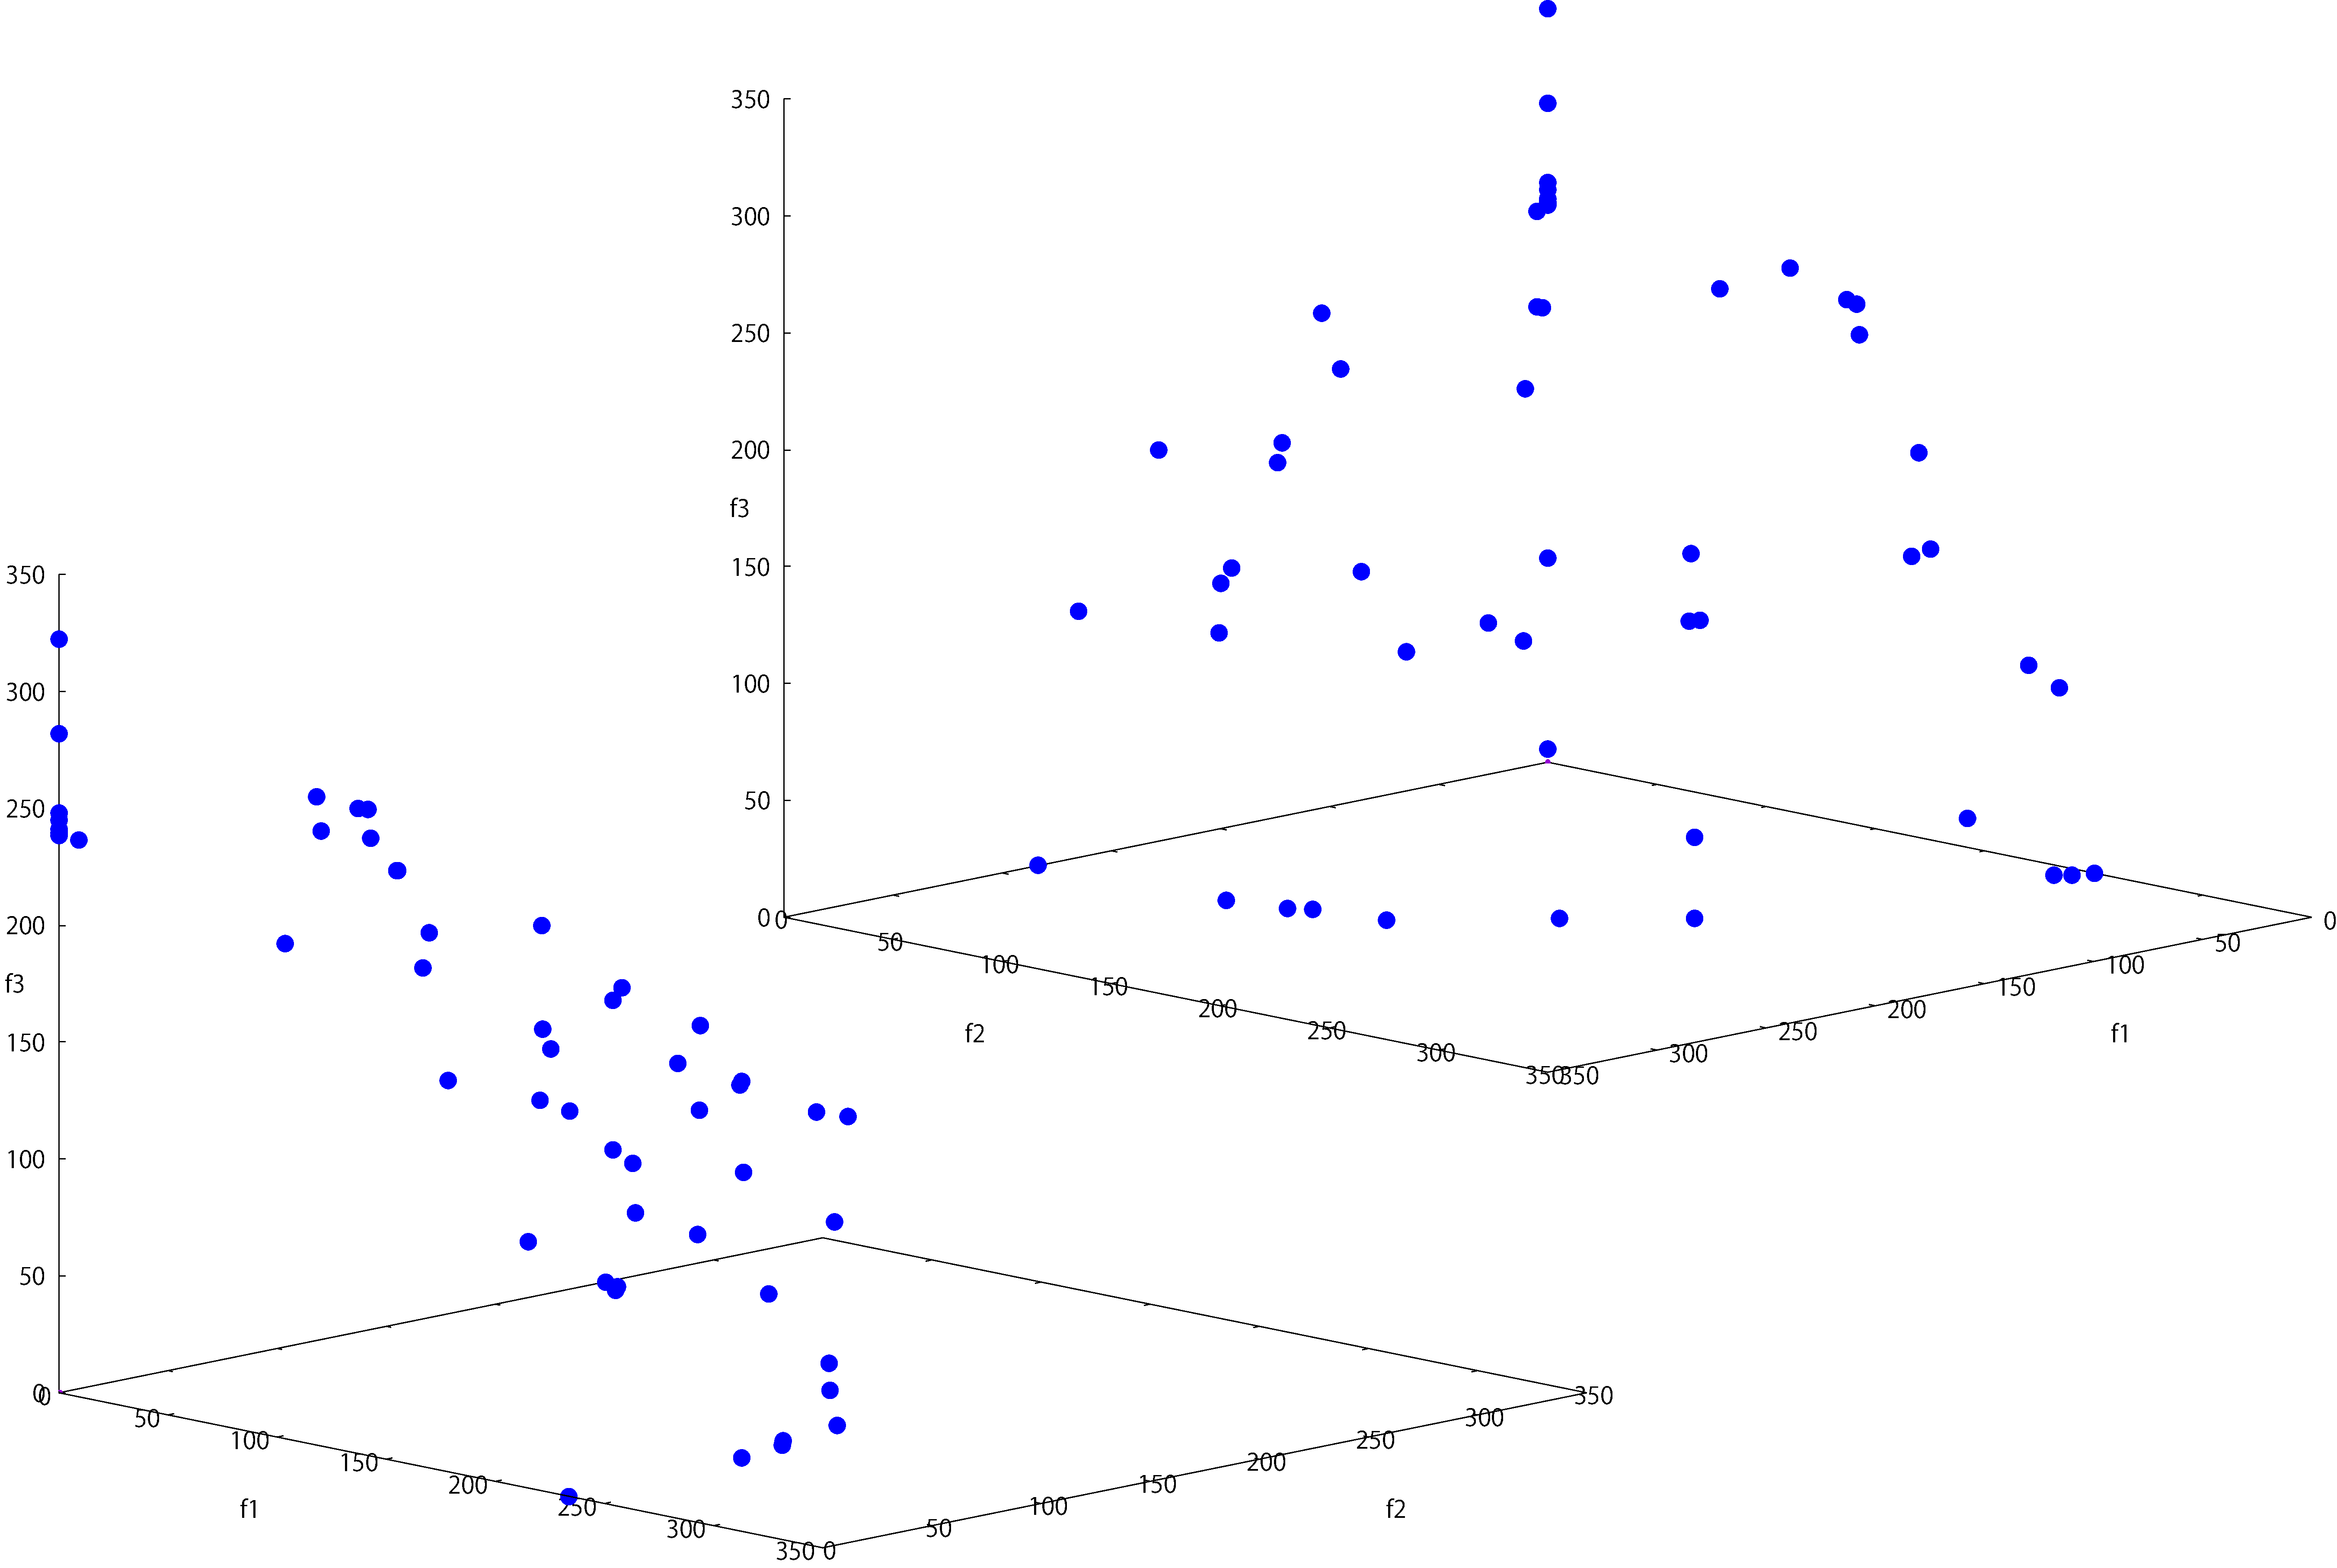
\includegraphics[width=1\linewidth]{../figures/MOEAD/DTLZ3_another_digi2_double.pdf}
\begin{center}
{\footnotesize (a) 2-digit resoution}
\end{center}
\end{minipage}
\begin{minipage}{0.32\hsize}
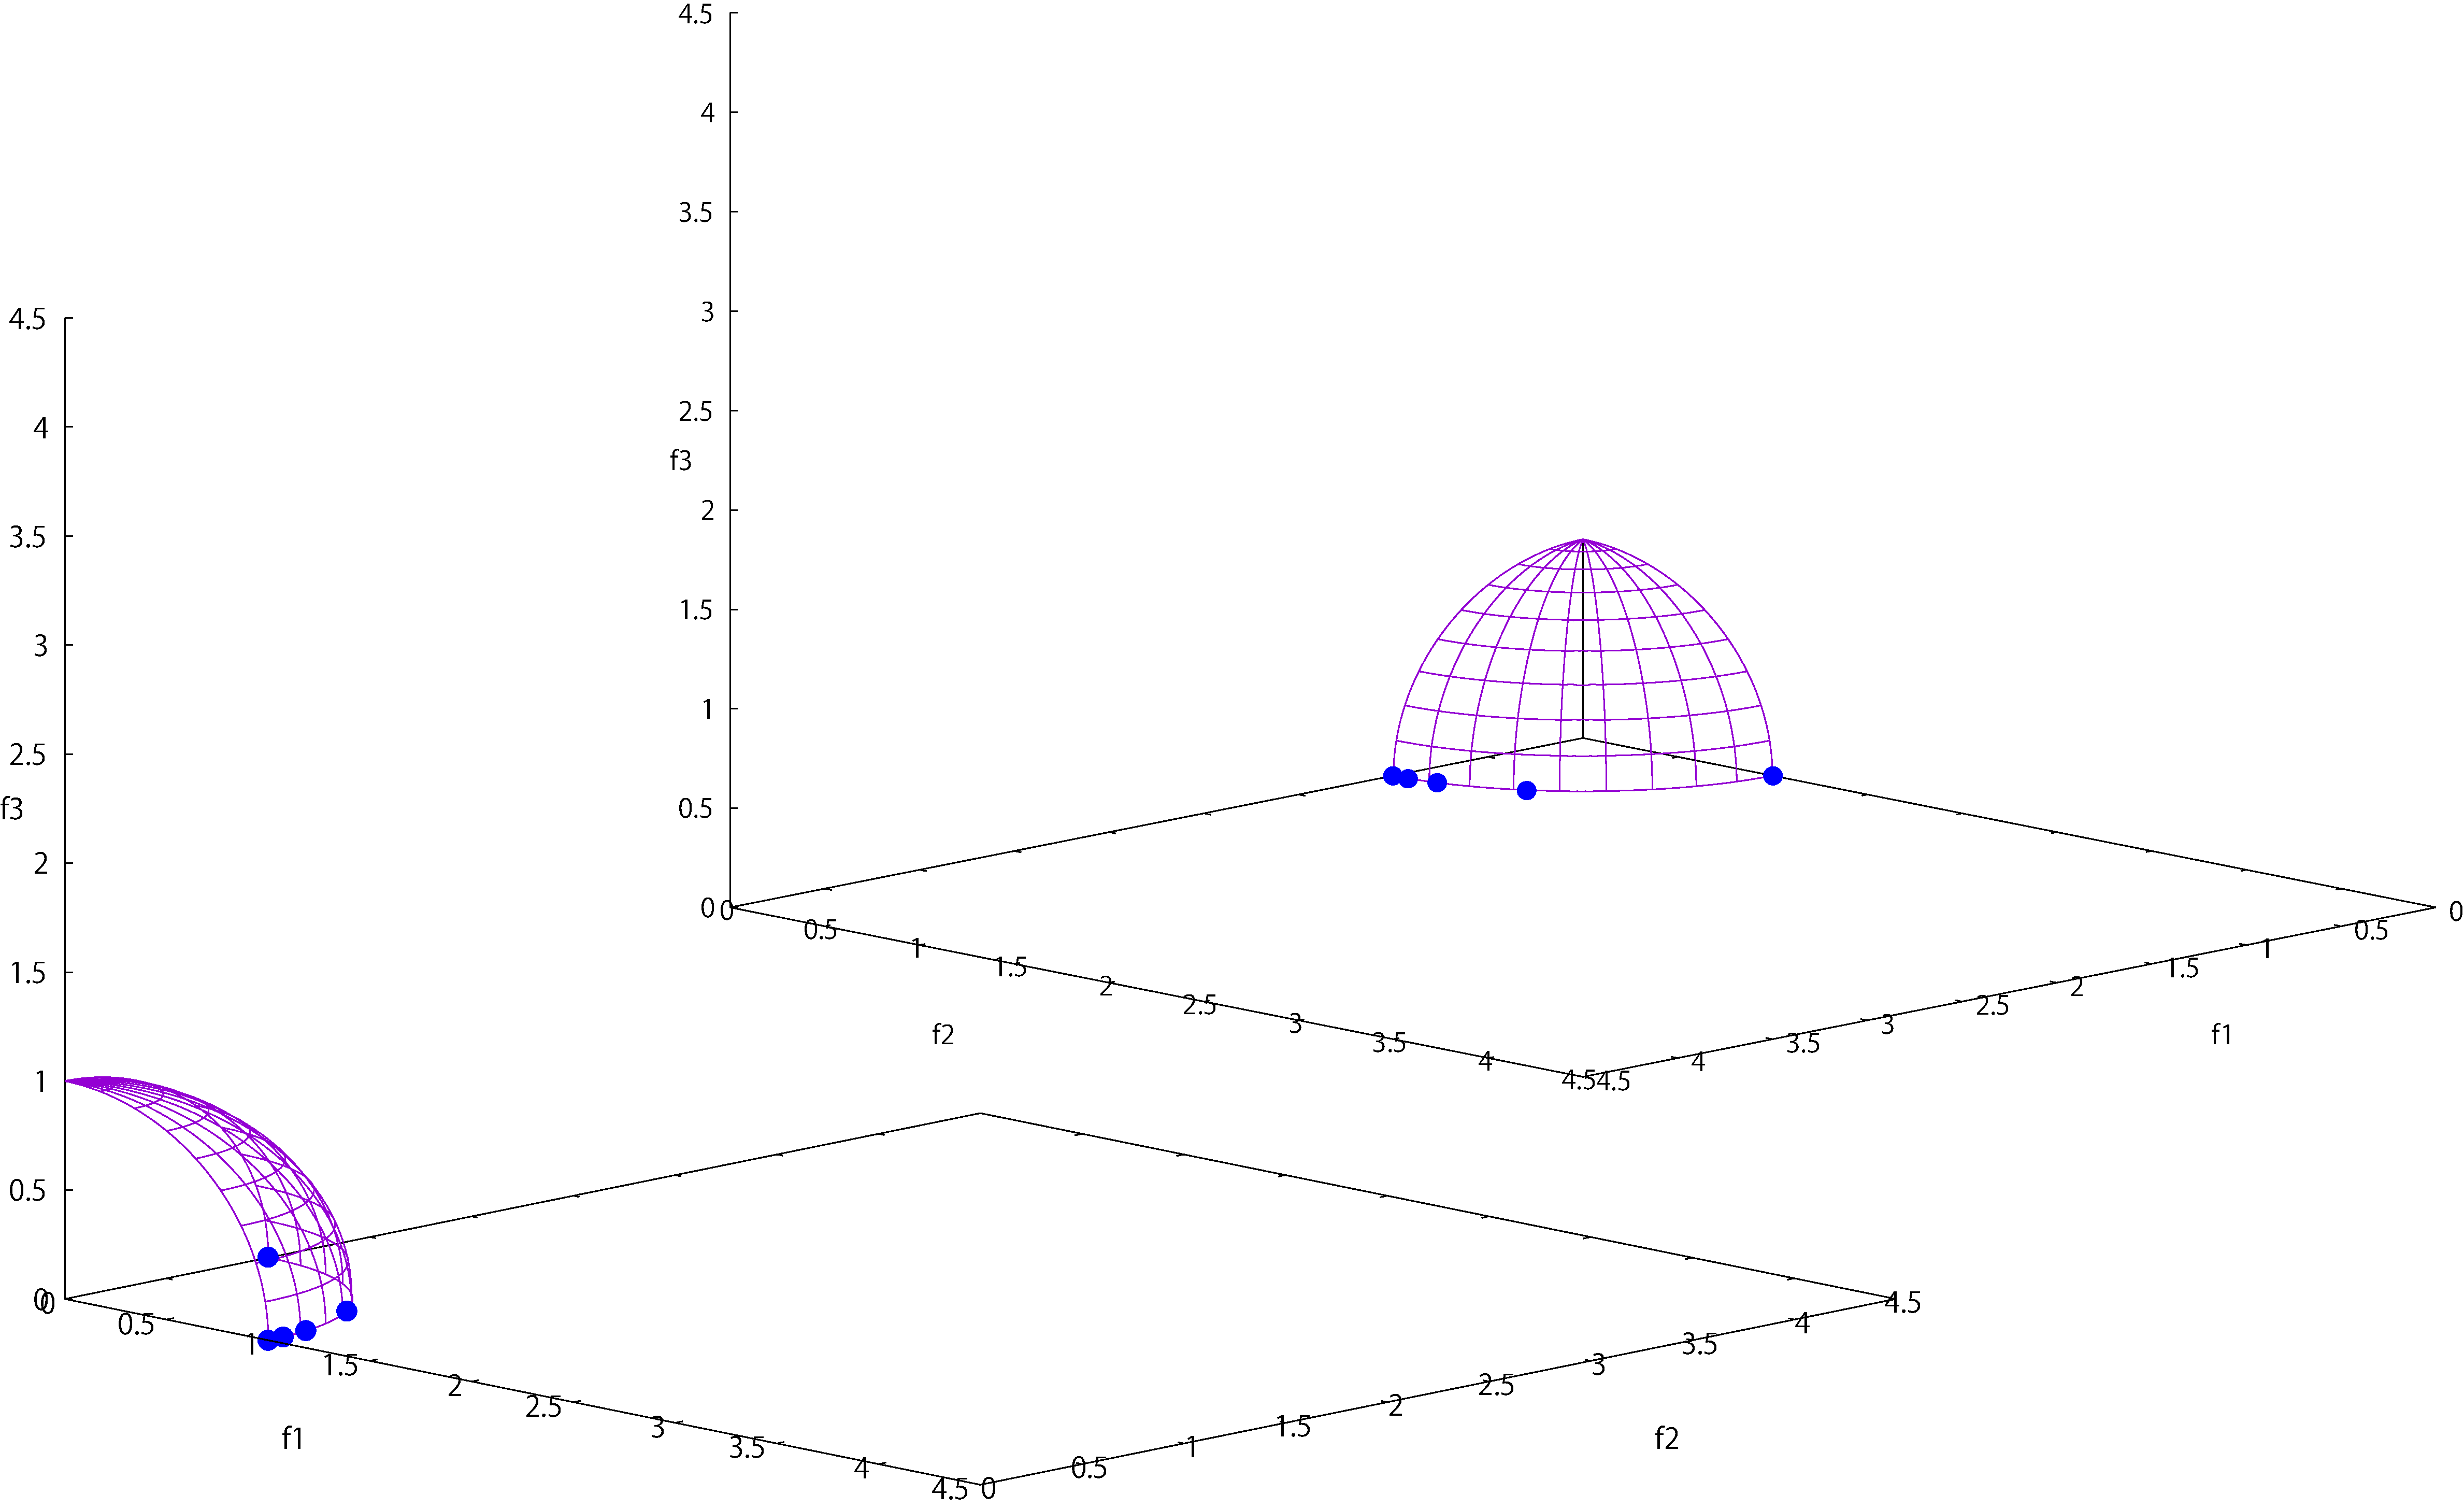
\includegraphics[width=1\linewidth]{../figures/MOEAD/DTLZ4_another_digi2_double.pdf}
\begin{center}
{\footnotesize (a) 2-digit resolution}
\end{center}
\end{minipage}
\end{tabular}
%\label{fig:dtlz4}
\end{figure*}

\begin{figure*}[htbp]
\begin{tabular}{cc}
\begin{minipage}{0.32\hsize}
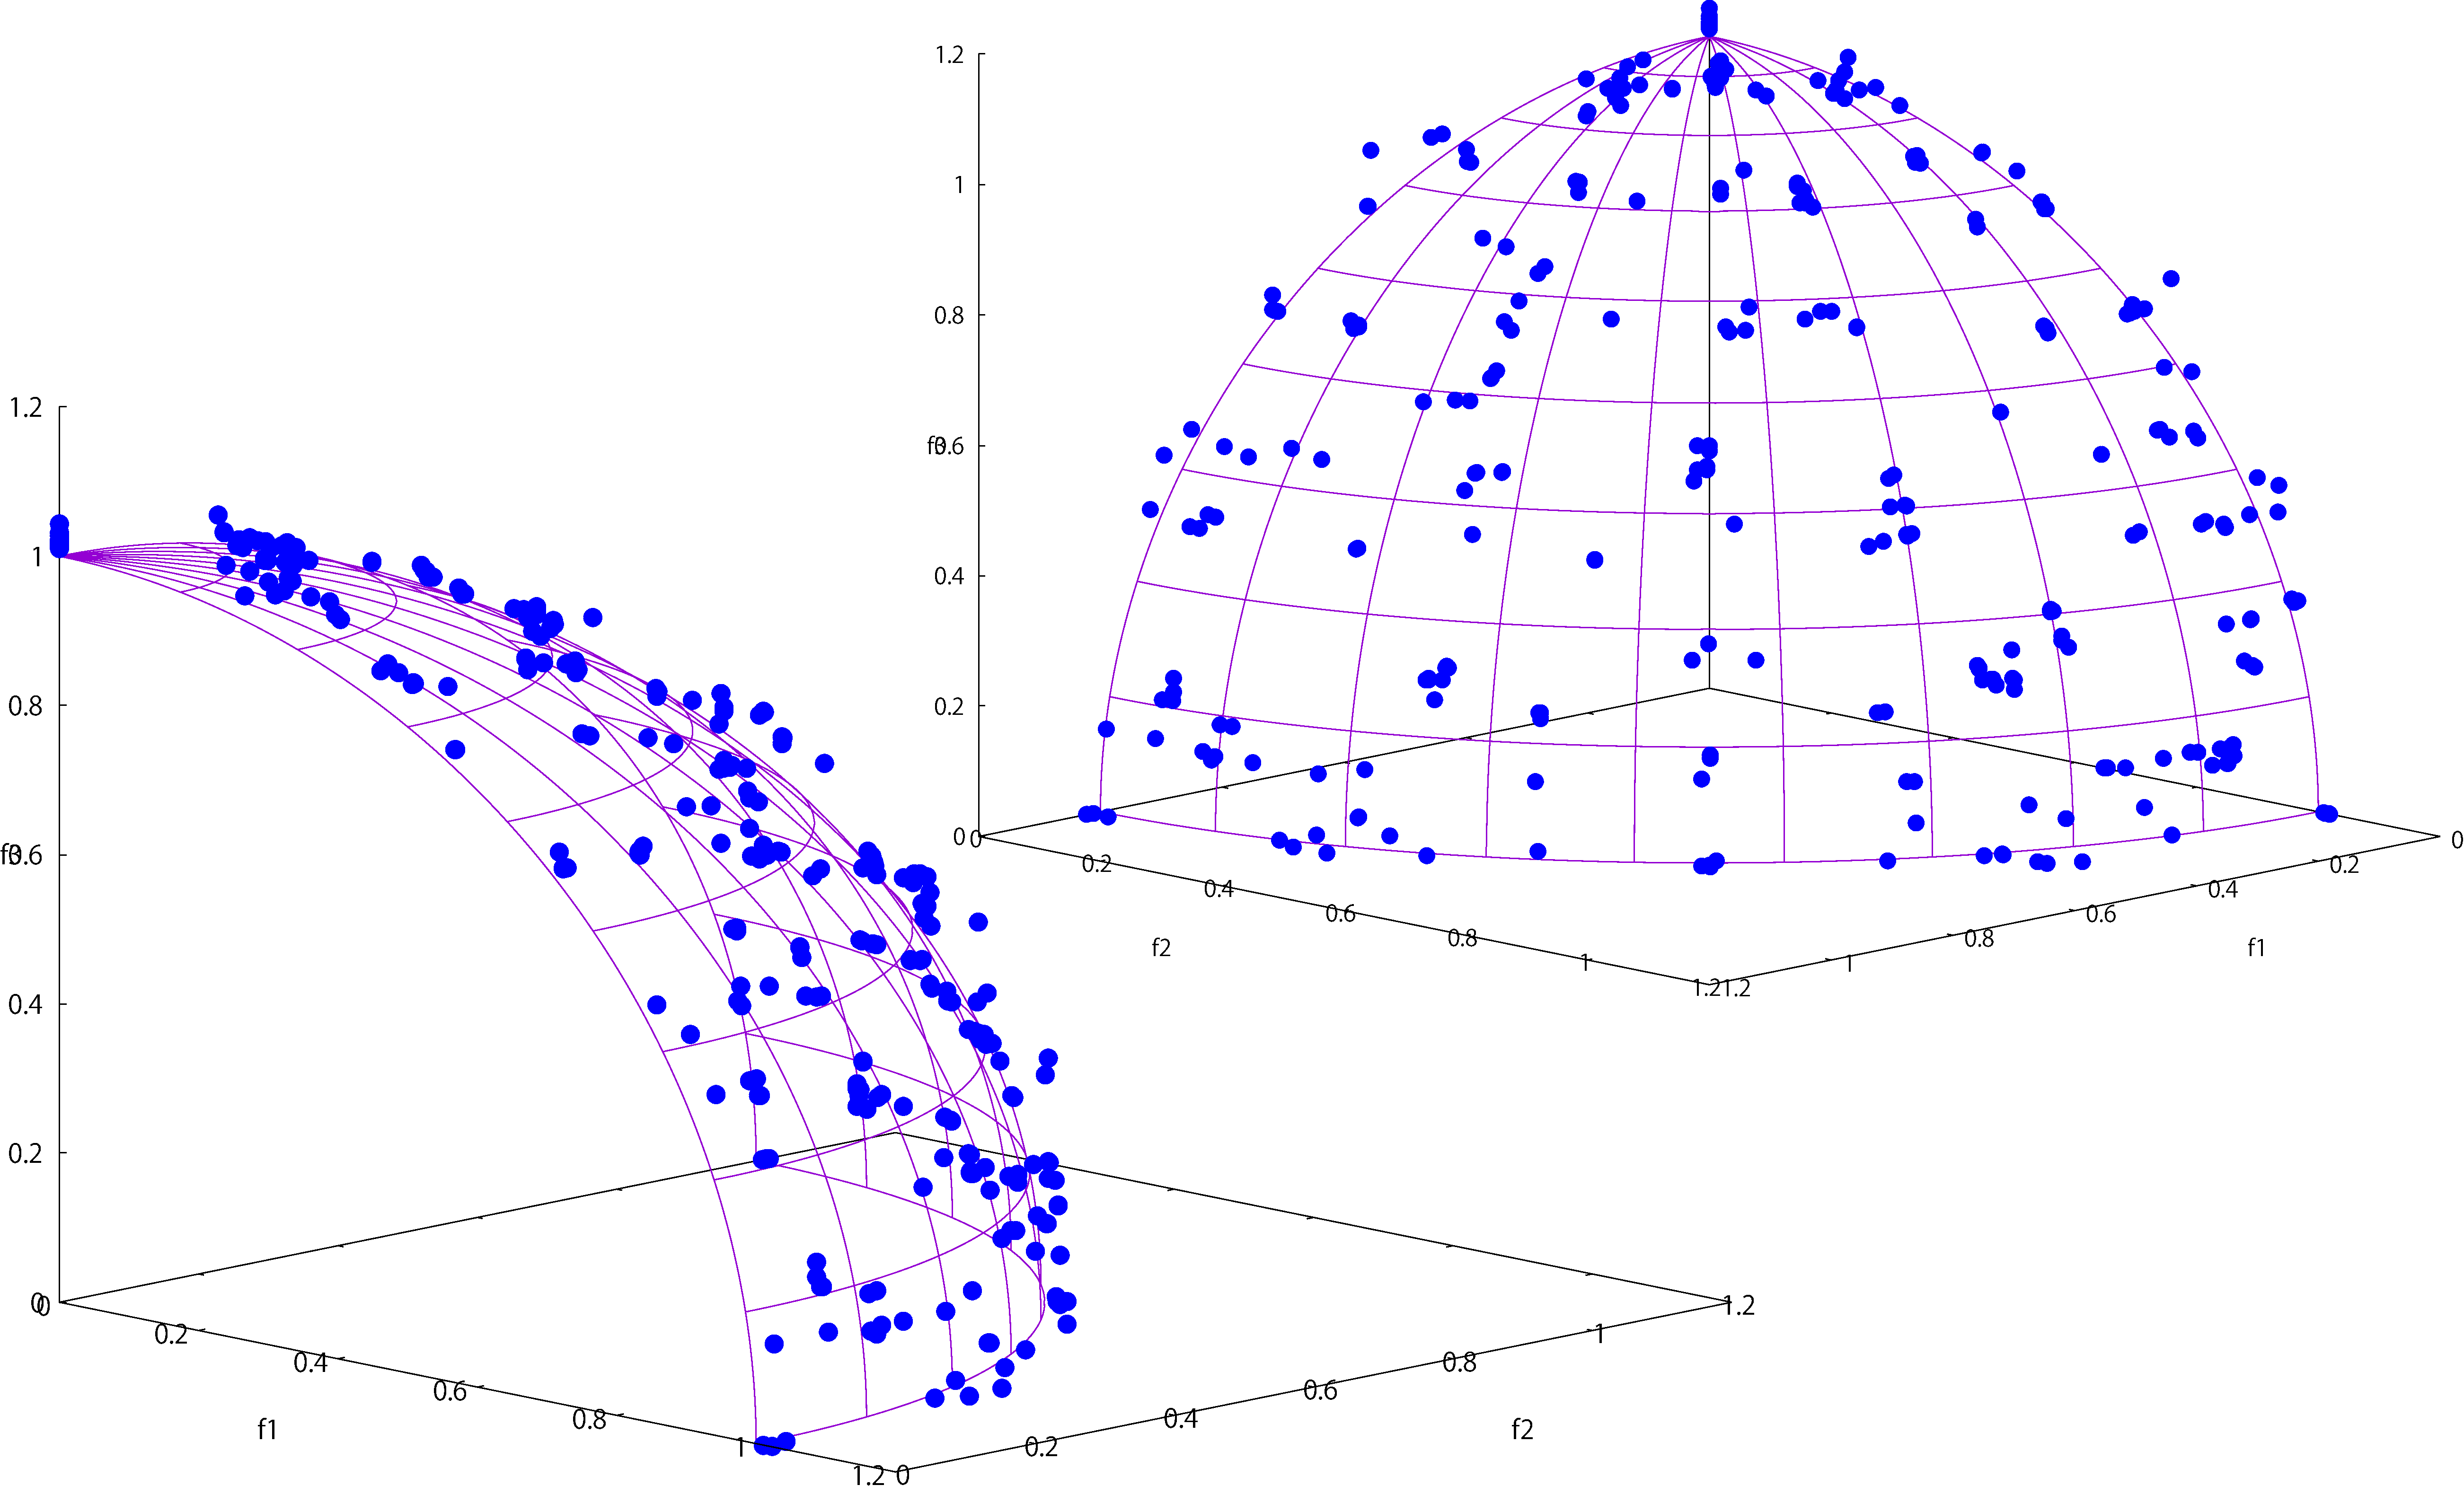
\includegraphics[width=1\linewidth]{../figures/MOEAD/DTLZ2_another_digi16_double.pdf}
\centering
{\footnotesize (b) 16-digit resoution}
\caption{Modified DTLZ2における非劣解の分布(MOEA/D)}
\label{moead_mod2_nondoms}
\end{minipage}
\begin{minipage}{0.32\hsize}
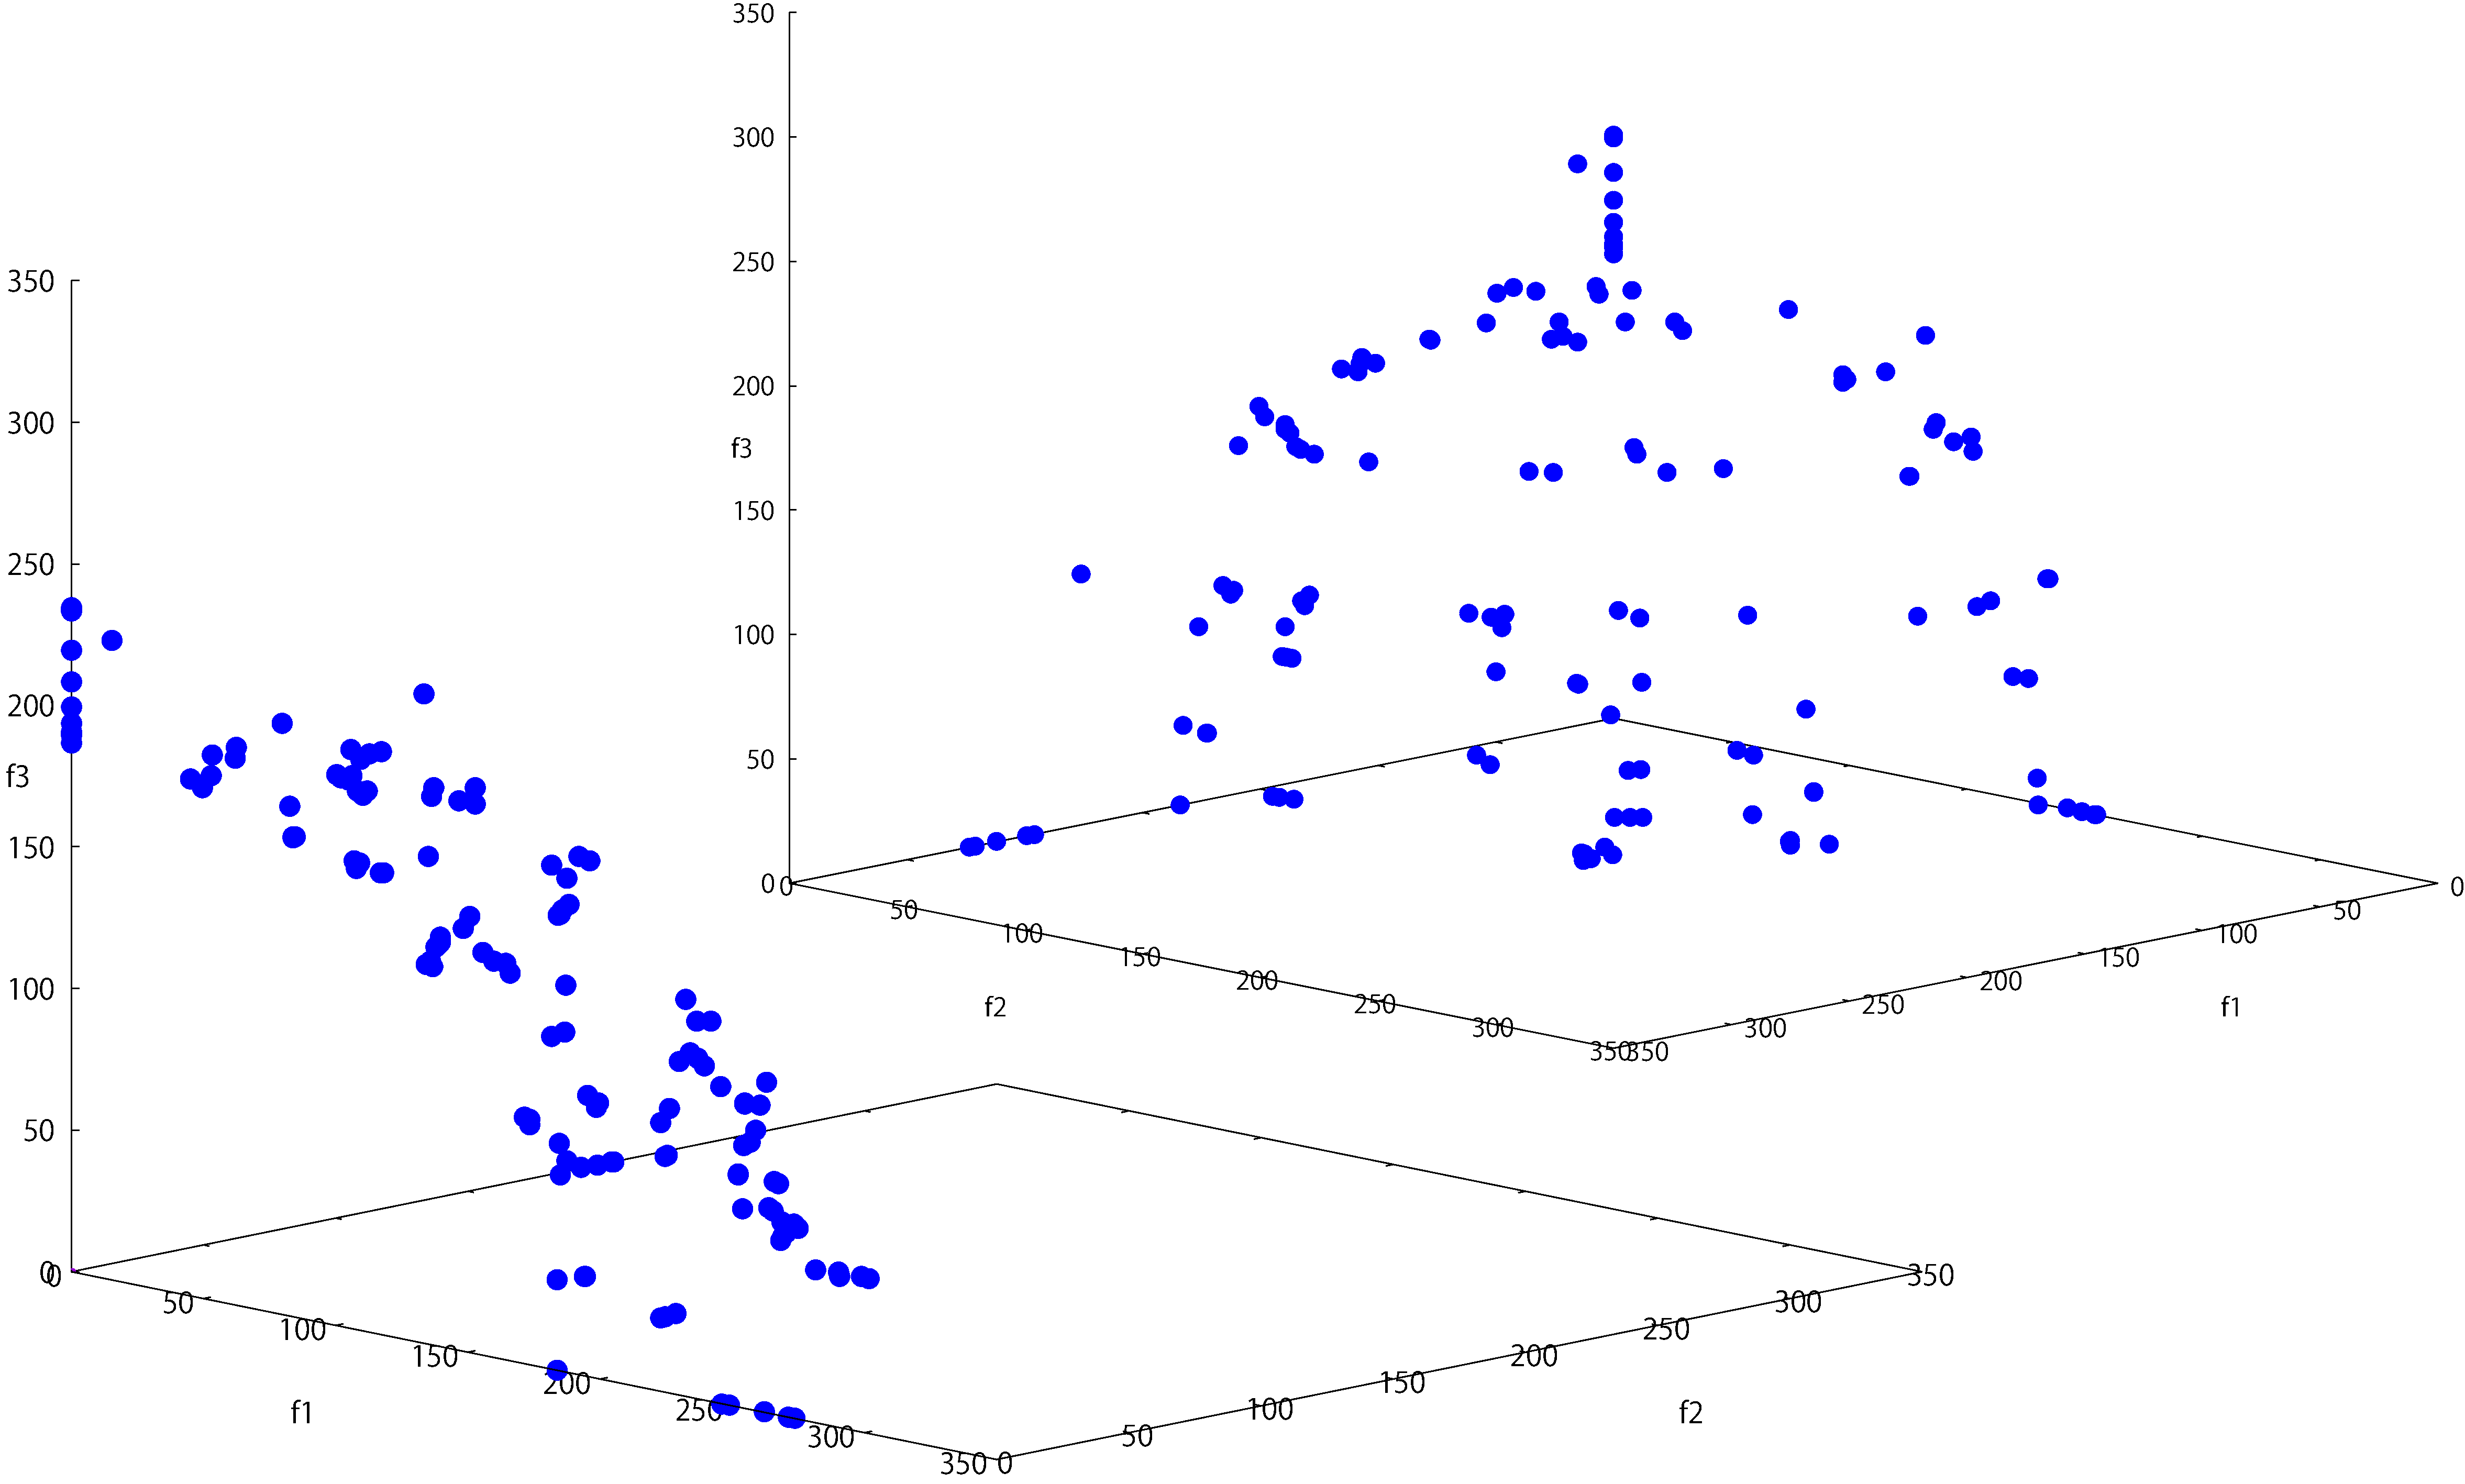
\includegraphics[width=1\linewidth]{../figures/MOEAD/DTLZ3_another_digi16_double.pdf}
\centering
{\footnotesize (b) 16-digit resolution}
\caption{Modified DTLZ3における非劣解の分布(MOEA/D)}
\label{moead_mod3_nondoms}
\end{minipage}
\begin{minipage}{0.32\hsize}
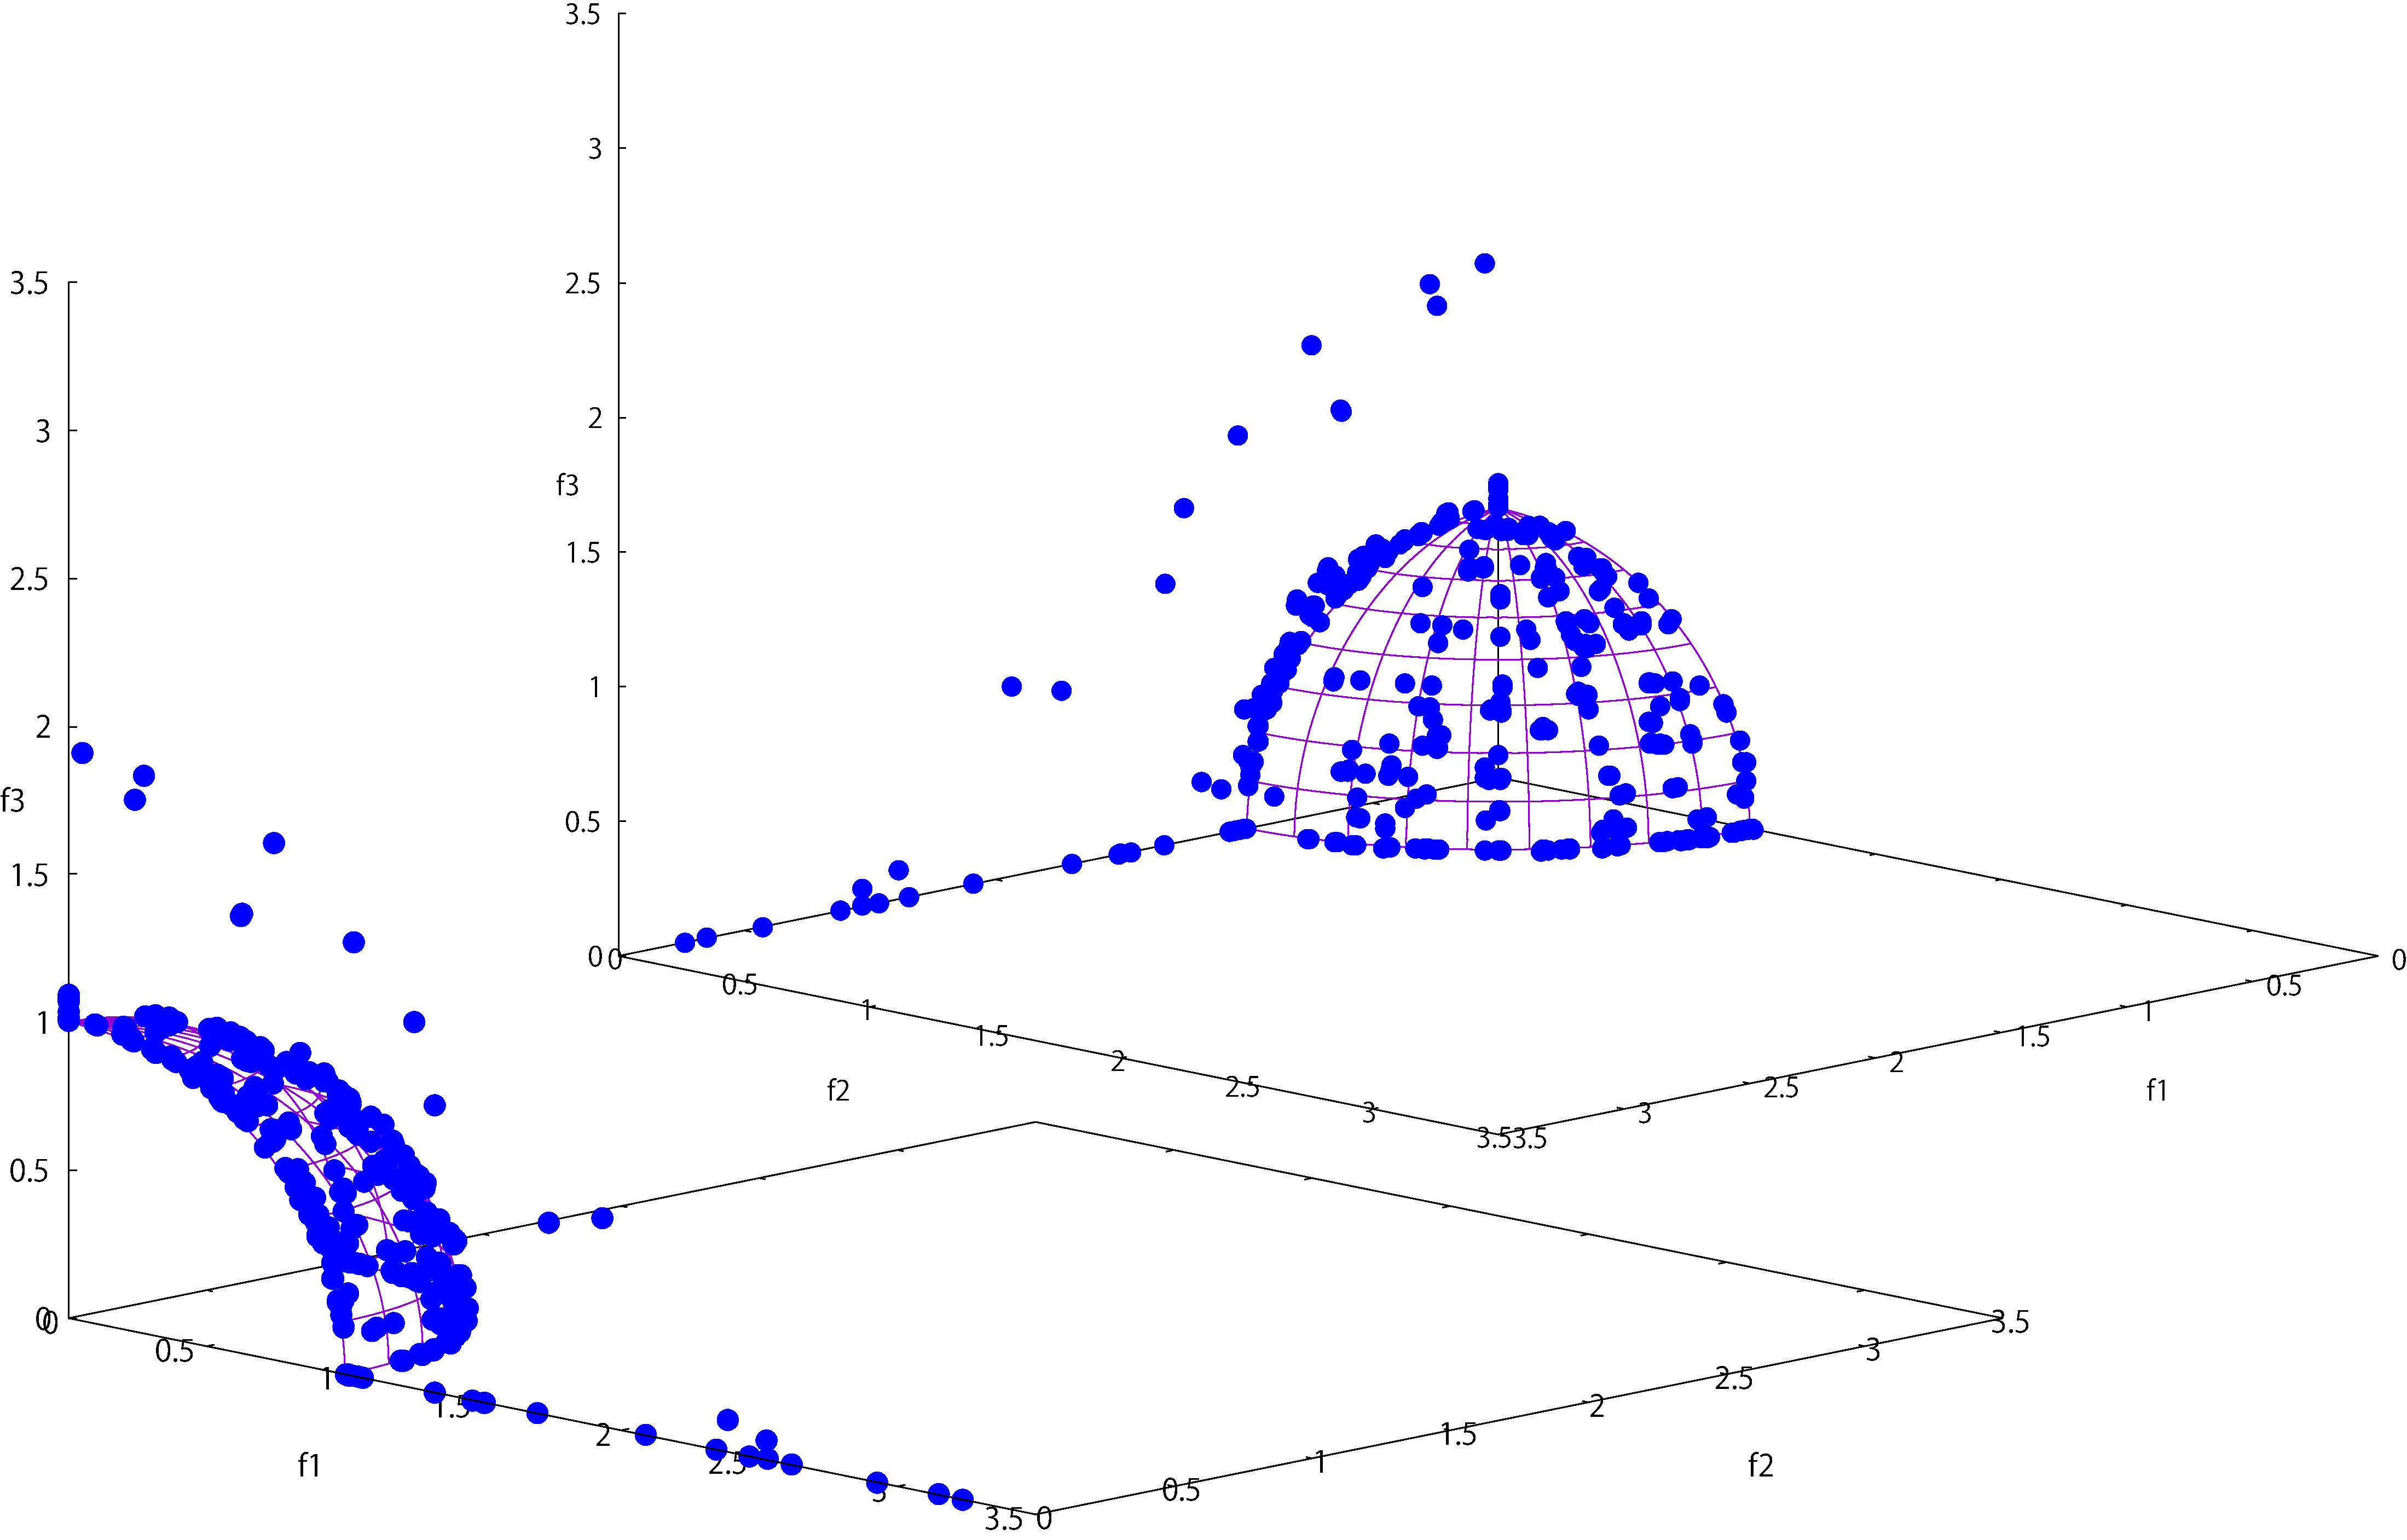
\includegraphics[width=1\linewidth]{../figures/MOEAD/DTLZ4_another_digi16_double.pdf}
\centering
{\footnotesize (b) 16-digit resolution}
\caption{Modified DTLZ4における非劣解の分布(MOEA/D)}
\label{moead_mod4_nondoms}
\end{minipage}
\end{tabular}
\end{figure*}

\afterpage{\clearpage}

\Figref{fig:igd_mod_moead}はModified DTLZ2-4のIGDの世代ごとの推移を示している.
\Figref{fig:igd_mod_moead}の結果から,Modified DTLZ3,4では桁数が小さいほど悪い結果となっていることが分かる.
このことからも,単に粗く離散化するだけでは解の多様性が失われてしまう可能性があることが分かる.

\Figref{moead_mod2_nondoms},\ref{moead_mod3_nondoms},\ref{moead_mod4_nondoms}は,それぞれ,Modified DTLZ2-4において2桁と16桁を用いた場合に得られた非劣解集合を示している.
\Figref{moead_mod2_nondoms}より,Modified DTLZ2においては,2桁と16桁で得られた非劣解集合に大きな差は見られなかった.
\Figref{moead_mod3_nondoms}では,どちらの桁数を似たような非劣解集合が得られているものの,16桁のほうがやや最適化方向である原点方向に進化が進んでいることが分かる.
NSGA-IIの結果で述べたように,Modified DTLZ3は無理数を最適値として取るため,設計変数に細かい粒度が必要とされる.
しかし,2桁では粒度が粗すぎるため,厳密な最適解に近付くことができず16桁よりも収束性が劣ってしまっていることが,非劣解集合からも確認できた.
\Figref{moead_mod4_nondoms}では,Modified DTLZ4においては,16桁は紫で示した真のパレートフロントを覆うように非劣解が得られているが,2桁では局所的にしか得られていないことが分かる.
先行研究のDTLZ4やNSGA-IIの結果と同様に2桁では多様性を維持するための必要最低限な設計変数の粒度を満たしておらず,解の多様性が悪化してしまったことが考えられる.

以上より,MOEA/Dにおいて,19の様々な特徴を持つベンチマーク問題を用いて設計変数の離散化の影響を幅広く評価した結果,NSGA-IIの結果と同様に,粗く離散化することで解の収束性が向上する傾向が確認された.
また,粗く離散化しすぎると問題によっては,解の収束性や多様性が失われてしまう可能性があることも確認された.
したがって,代表的なRCGAであるNSGA-IIとMOEA/Dにおいては,問題ごとに各設計変数を適切に離散化することで,解の多様性を維持しながらも,収束性を高めることができる可能性があることが分かった.
%
%以上より,NSGA-IIにおいて,19の様々な特徴を持つベンチマーク問題を用いて設計変数の離散化の影響を幅広く評価した結果,先行研究と同様に粗く離散化することで解の収束性が向上する傾向が確認された.
%また,粗く離散化しすぎると問題によっては,解の収束性や多様性が失われてしまう可能性があることが分かった.
%したがって,NSGA-IIにおいては,問題ごとに各設計変数を適切に離散化することで,解の多様性を維持しながらも,収束性を高めることができる可能性があることが分かった.
%
%


\section{設計変数の離散化による影響評価のまとめ}
\quad 本実験では,先行研究では明らかにできなかった実数値遺伝的アルゴリズムにおける設計変数の離散化が探索に及ぼす影響の一般性を幅広く評価した.
ここでは,実数値遺伝的アルゴリズムとして代表的な二つのアルゴリズム(NSGA-II,MOEA/D)と様々な特徴を持つ19のベンチマーク問題を用いて,設計変数の離散化の影響を解の収束性・多様性の観点から評価した.

NSGA-IIの結果から,多くの問題で設計変数を粗く離散化するほど解の収束性が向上するが,問題によっては粗く離散化しすぎると解の収束性と多様性が悪化してしまう可能性があることが分かった.
また,MOEA/Dの結果においてもNSGA-IIと同様の傾向が見られた.

以上より,RCGAにおいて問題に応じて各設計変数に適切な離散化を行うことで,解の多様性を維持しながらも収束性を向上させることが期待される.
実際の設計問題では,目的関数や制約条件の計算に莫大な計算資源や計算時間がかかる場合があるため,効率的な探索手法が求められている.
この課題を解決するアプローチの一つとして,設計変数の離散化が有効に働くことが期待できる.
しかし,先行研究と同様に,最適化の前に適切に設計変数を離散化することは難しく,設計変数の離散化の有効な活用法としては課題が残されている.


\end{document}